
\documentclass[b5paper]{tbook}
\usepackage{ascmac}
\usepackage{shiika}
\usepackage{kyakuchu}
\usepackage{multicol}
\usepackage{furikana}
\usepackage[dvipdfmx]{graphicx}
\begin{document}
\author{吉川ふみ子}
\title{ふみこ句日記}
\date{2000/5/51}
\maketitle
\tableofcontents
\chapter*{はじめに}
���a�l�\���N�㌎���[�q����ƎO������ւ̎Ԓ��A
�R�����q�ɏo��ЎO���̕a�@�ɗ×{���̑�˂����������
�����������@�b�͋g������o�̂����߂ɂ��
�����q�Ηj�����ɐ�삳��@���c���q���񂪓���


�㌎�����ɏo�Ȃ����l�q�������B
�����ꂩ��������ā@�\�����Ƃ������o�債���B

���鏑���ƌ������Ƃɂ͑S�X���M�̂Ȃ��o��������
���܂�i�񂾋C�����ł́v�Ȃ��������B
�ȗ��@�����~�߂���J��Ԃ����B
��������ւ̋`���𑱂��Ă���ƌ������B

�����ď\���N�̔N�����߂����B�[���̂��������̋�
��͖w��ǖ����B

�l�ŋ�W�����ꂽ��F�����l�����邪�@�Ηj�΋��@������W��
���ԓ��肪����t�̂��ƁA����ȏ㎩���̋�������ɂ̂������Ƃ�
�l���Ă����Ȃ������B����ǂ������N�O�������L�Ƃ��ā@����
���Ă݂悤�Ǝv���������B
����A��ɂȂ��Ă��Ȃ���@����ł悢�B�v���΂���łȂ��Ȃ�
�Ƃ肩����Ȃ��Ł@��A�O�N�͉߂����B

����@�ʑ�����@�����N����ف@�ۗ{�z�[���ɓ����@�R������@�x�q����
�ƍ�������܂ł̈�T�ԁ@��l�̋@�𓾂đQ����ł������o���n�߂�B
�U��Ԃ茩��\���N�@�L���m���łȂ����������邪
�v���o�͊y�����G


\hfill {  \rensuji*{3} �E \rensuji* {8} �E  \rensuji*[1]{26}}

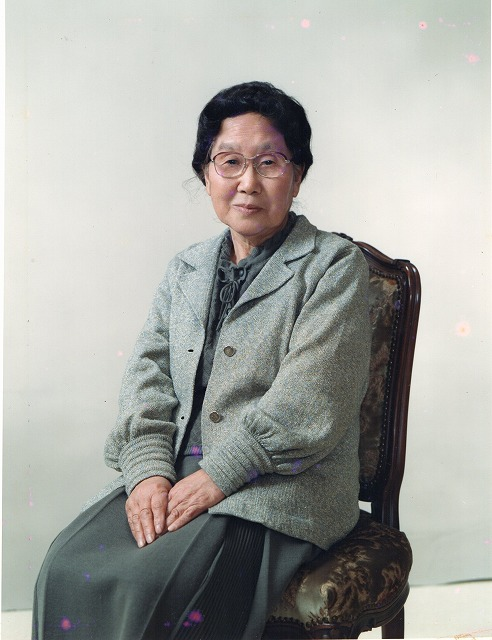
\includegraphics[height=10cm, angle=90, bb=0 0 640 640]{cat.jpg}
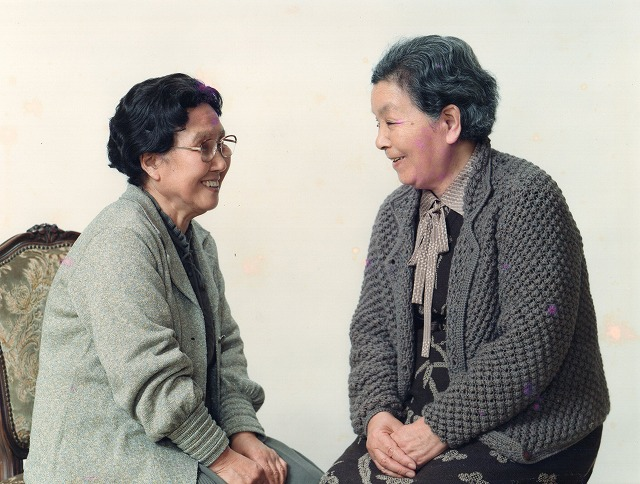
\includegraphics[height=10cm, angle=90, bb=0 0 640 640]{fumiko2.jpg}
\chapter{野仏}


 
吉祥会で大森先生 池永先生に一緒に当尾の石仏を巡りて 

\begin{shiika}
野仏の笑ひ在せり 曼珠沙華\hfill { \rensuji*{48} ・ \rensuji* {8} }
\end{shiika}
\vspace{0.6cm}
「草紅葉」兼題 幼き日の思い出 
\begin{shiika}
 日を浴びてままごとの子や草紅葉\hfill { \rensuji*{48} ・ \rensuji* {10} }
\end{shiika}
\vspace{0.6cm}
「顔見世」 去年は文友会で顔もせに。今年はただ思い出のみ
\begin{shiika}
顔見世の名残を夢に見しも去年\hfill { \rensuji*{48} ・ \rensuji* {12} ・}
\end{shiika}
\vspace{0.6cm}
お隣の浅野まゆみさんかわいい日本髪で
\begin{shiika}
髪結ひて寝ず娘は待つ初詣\hfill { \rensuji*{49} ・ \rensuji* {1} ・}
\end{shiika}
\vspace{0.6cm}
相川北通りの家根笹の中で狂い猫
\begin{shiika}
猫の恋根笹の乱れ昨日今日\hfill { \rensuji*{49} ・ \rensuji* {2} ・}
\end{shiika}
\vspace{0.6cm}
上京の車中 
浜松あたりで遠連山をみて
\begin{shiika}
山の色幾重の果の雪解光\hfill { \rensuji*{49} ・ \rensuji* {2} ・ }	
\end{shiika}
\vspace{0.6cm}
\begin{shiika}野仏の笑ひ在せり曼珠沙華
\hfill{\rensuji*{48}・\rensuji*{9}・\rensuji*{0}}\end{shiika}
\vspace{0.6cm}
「水草生まふ」 兼題 日浅い私には大変むつかしい。ふと一善の
車で探梅につれてもらった時\\賀名生 だったかそして仁徳陵ところを走ったことを
思い出す。
\begin{shiika}陵の薄陽の濠も水草生ふ
\hfill{\rensuji*{49}・\rensuji*{3}・\rensuji*{0}}\end{shiika}



\vspace{0.6cm}
「春の雪」兼題 直子さんの縁談がまた立ち消えた。
\begin{shiika}娘の縁談又もこわれぬ春の雪
\hfill{\rensuji*{49}・\rensuji*{3}・\rensuji*{0}}\end{shiika}

\vspace{0.6cm}
一つの旅を終えるとまた次に心は走る。
\begin{shiika}花過ぎぬいづこともなき旅心
\hfill{\rensuji*{49}・\rensuji*{4}・\rensuji*{0}}\end{shiika}
\vspace{0.6cm}
「桐の花」兼題 小森田さんとあわくら荘に 帰りは姫路までバスにした。
\begin{shiika}山裾の雨に煙れる桐の花
\hfill{\rensuji*{49}・\rensuji*{5}・\rensuji*{0}}\end{shiika}
\vspace{0.6cm}
「草の花」兼題どこで得た句かはっきりしない。
\begin{shiika}野仏の顔かくすまで草の花
\hfill{\rensuji*{49}・\rensuji*{9}・\rensuji*{0}}\end{shiika}
\vspace{0.6cm}
山下さん 小森田さん 青山さん 四人連れ 児玉東洋さんの
車で佐多岬 桜島 霧島と廻っていただく。\\別れて高千穂の
国民宿舎に泊った夜 高千穂神社の夜神楽をみに行く。
\begin{shiika}夜神東の明りに映ゆる銀杏黄葉
\hfill{\rensuji*{49}・\rensuji*{11}・\rensuji*{0}}\end{shiika}
\vspace{0.6cm}
「炬燵」兼題 一人暮らしの私の句だと浅野さんの御主人がはやす
\begin{shiika}置炬燵向ふ人なきあで蒲団
\hfill{\rensuji*{49}・\rensuji*{11}・\rensuji*{0}}\end{shiika}
\vspace{0.6cm}
「年用意」丹波から週二回野菜その他を積んで車が来る大塚「きく」
の前でとまる。\\ 大塚ののぶ子さんが電話で「丹波よ」と相川の店へしらせてくれる。
\begin{shiika}年用意丹波男の荷は売れ早き
\hfill{\rensuji*{49}・\rensuji*{12}・\rensuji*{0}}\end{shiika}
\vspace{0.6cm}
\vspace{0.6cm}
小森田さんが名古屋から夕方までに相川へ着く筈になっているのに
遅い
\begin{shiika}友待つに暮色刻々粉雪舞ふ
\hfill{\rensuji*{50}・\rensuji*{1}・\rensuji*{0}}\end{shiika}
\vspace{0.6cm}
上京車窓より。
\begin{shiika}風ぬくき末黒野烏群をなし
\hfill{\rensuji*{50}・\rensuji*{2}・\rensuji*{0}}\end{shiika}
\vspace{0.6cm}
私は化粧水は使っていないが ふと出来た句
\begin{shiika}化粧水掌に冷えのなし春隣
\hfill{\rensuji*{50}・\rensuji*{3}・\rensuji*{0}}\end{shiika}
\vspace{0.6cm}
「花曇」野崎詣りをしらのは去年だったかと思う。
\begin{shiika}綿菓子も売れて野崎の花曇
\hfill{\rensuji*{50}・\rensuji*{4}・\rensuji*{0}}\end{shiika}
\begin{shiika}花曇年甲斐もなき物忘れ
\hfill{\rensuji*{50}・\rensuji*{4}・\rensuji*{0}}\end{shiika}
\vspace{0.6cm}
この様な軽やかな心に時もある
\begin{shiika}若やぎて夏来る歌口ずさむ
\hfill{\rensuji*{50}・\rensuji*{0}・\rensuji*{5}}\end{shiika}
\vspace{0.6cm}
相川の家の軒に雀がいそかしげに出入りする
\begin{shiika}梅雨曇出入せはしき軒雀
\hfill{\rensuji*{50}・\rensuji*{6}・\rensuji*{0}}\end{shiika}
\vspace{0.6cm}
相川の町の露地風景
\begin{shiika}花曇年甲斐もなき物忘れ
\hfill{\rensuji*{50}・\rensuji*{6}・\rensuji*{0}}\end{shiika}
\vspace{0.6cm}
どこの寺院だったかなー
\begin{shiika}あらはなるちくり根洗ひ大夕立
\hfill{\rensuji*{50}・\rensuji*{7}・\rensuji*{0}}\end{shiika}
\vspace{0.6cm}
「流れ星」この頃誰かが病気をして心にかかっていた
\begin{shiika}看る夜の心もとなき星の飛ぶ
\hfill{\rensuji*{50}・\rensuji*{8}・\rensuji*{26}}\end{shiika}
\vspace{0.6cm}
「空蝉」故かんげつ国分寺境内の礎石で遊んだ日をおもいだして
\begin{shiika}子等去りぬ礎石にならぶ蝉の殻
\hfill{\rensuji*{50}・\rensuji*{8}・\rensuji*{0}}\end{shiika}
\vspace{0.6cm}
唐招提寺 観月の夜
\begin{shiika}大月夜唐招提寺の庭に彳つ
\hfill{\rensuji*{50}・\rensuji*{9}・\rensuji*{0}}\end{shiika}
\vspace{0.6cm}
「色鳥」山下さん青山さんと越前賤ケ岳 長浜竹生島の旅
\begin{shiika}色鳥や朝の湖の小桟橋
\hfill{\rensuji*{50}・\rensuji*{10}・\rensuji*{0}}\end{shiika}
\vspace{0.6cm}
「秋惜しむ」小森田さんと笑い乍らの出来たもの
\begin{shiika}秋惜しむほほ紅少こしさしてみむ
\hfill{\rensuji*{50}・\rensuji*{10}・\rensuji*{0}}\end{shiika}
\vspace{0.6cm}
大塚さん「きく」の前に荷をおろす「丹波」のこと
\begin{shiika}新鮮と我から言ひて冬菜売
\hfill{\rensuji*{50}・\rensuji*{12}・\rensuji*{0}}\end{shiika}
\vspace{0.6cm}
相川の座敷の庭に笹子
の声がと井上さんからきく
\begin{shiika}独り居の朝茶の香り笹に来る
\hfill{\rensuji*{51}・\rensuji*{1}・\rensuji*{0}}\end{shiika}
\vspace{0.6cm}
「大福茶」我が家は梅昆布茶が毎年のこと大福茶と
思っている。
\begin{shiika}家長の座に心しまりて大福茶
\hfill{\rensuji*{51}・\rensuji*{1}・\rensuji*{0}}\end{shiika}
\vspace{0.6cm}
「野焼き」 あちこちに見る野火に次の命の芽生えを思った。
\begin{shiika}新らしき命を呼びて野火勢ふ
\hfill{\rensuji*{51}・\rensuji*{2}・\rensuji*{0}}\end{shiika}
\vspace{0.6cm}
「春泥」 浄瑠璃寺への柊が浮かんできた。 そして遠足の
列が眼に入る。
\begin{shiika}春泥の径つき寺の小門あり
\hfill{\rensuji*{51}・\rensuji*{3}・\rensuji*{0}}\end{shiika}
\begin{shiika}黄帽子水筒どの児の靴も春の泥
\hfill{\rensuji*{51}・\rensuji*{3}・\rensuji*{0}}\end{shiika}
\vspace{0.6cm}
高山祭をめざして小森田さん 美佐さん 宮川ひでさんと下呂
へ行く。折り悪し雨で宵の「曳別れ」は
みることができなかったが車窓より禅昌寺の塔を眺めて
\begin{shiika}花の奥雨に煙れる塔のあり
\hfill{\rensuji*{51}・\rensuji*{4}・\rensuji*{0}}\end{shiika}
\vspace{0.6cm}
小森田」さん 高田さんと妙高々原 穂高 と旅して 穂高の
有明松尾寺にて、妙高々原にて
\begin{shiika}老鶯や御手の茶壺のかたむける
\hfill{\rensuji*{51}・\rensuji*{5}・\rensuji*{0}}\end{shiika}
\begin{shiika}老鴬に唐松林行きにゆく
\hfill{\rensuji*{51}・\rensuji*{5}・\rensuji*{0}}\end{shiika}
「落し文」 むつかしい兼題にふと昨年の賤ケ岳を思い出して
\begin{shiika}湖見ゆる古戦場道落し文
\hfill{\rensuji*{51}・\rensuji*{7}・\rensuji*{0}}\end{shiika}
\vspace{0.6cm}
亡妹貞子が死の近くなった頃
梨をしきりにほしがった。梨の頃がくると思い出す。
\begin{shiika}病妹の欲りし日とあり梨供ふ
\hfill{\rensuji*{51}・\rensuji*{9}・\rensuji*{0}}\end{shiika}
\vspace{0.6cm}
京都女専クラス会 九州志賀島 大宰府 柳川巡りにて
\begin{shiika}鐘楼に屋根草のびて露ふかし
\hfill{\rensuji*{51}・\rensuji*{10}・\rensuji*{17}}\end{shiika}
\begin{shiika}四つ手網死魚の乾けり秋の声
\hfill{\rensuji*{51}・\rensuji*{10}・\rensuji*{17}}\end{shiika}
\vspace{0.6cm}
「晩菊」相川の庭の菊 謡の小川先生のこと。
\begin{shiika}晩菊のうつろいはじむ白きより
\hfill{\rensuji*{51}・\rensuji*{11}・\rensuji*{0}}\end{shiika}
\begin{shiika}晩菊やなほ美くしき謡の師
\hfill{\rensuji*{51}・\rensuji*{11}・\rensuji*{0}}\end{shiika}
\vspace{0.6cm}
耳の治療で大手町病院に通っていた頃
\begin{shiika}晩菊やなほ美くしき謡の師
\hfill{\rensuji*{51}・\rensuji*{11}・\rensuji*{0}}\end{shiika}
\vspace{0.6cm}
天満マーチャンダイズあたりにて
\begin{shiika}秋冷ゆる赤きストビラ散る舗道
\hfill{\rensuji*{51}・\rensuji*{11}・\rensuji*{0}}\end{shiika}
\vspace{0.6cm}
相川の庭の垣をみて。
\begin{shiika}綿虫の籬越え来て雨を呼ぶ
\hfill{\rensuji*{51}・\rensuji*{11}・\rensuji*{0}}\end{shiika}
\vspace{0.6cm}

\chapter{水無瀬}
西川さん 増田さん と淡路島健和荘泊り 灘水仙郷 若人も森など巡る。\\
帰途乗船場にて浅利貝を買う。
\begin{shiika}蛤の潮のしたたり出船待つ
\hfill{\rensuji*{52}・\rensuji*{3}・\rensuji*{0}}\end{shiika}
\vspace{0.6cm}
東横線多摩川鉄橋通過
\begin{shiika}河原なる飛球の行方風光る
\hfill{\rensuji*{52}・\rensuji*{3}・\rensuji*{0}}\end{shiika}
\vspace{0.6cm}
小田さんの案内で山下さんと三人で吉野山へ
\begin{shiika}吉野山春蘭の店は客呼ばず
\hfill{\rensuji*{52}・\rensuji*{4}・\rensuji*{5}}\end{shiika}
\vspace{0.6cm}
相川の畑にて
\begin{shiika}花弁ゆれ奥より出でし虻の貌
\hfill{\rensuji*{52}・\rensuji*{4}・\rensuji*{0}}\end{shiika}
\vspace{0.6cm}
相川の店二階の軒先に燕巣をつくる
\begin{shiika}燕の子黄ならびの嘴花のごと
\hfill{\rensuji*{52}・\rensuji*{5}・\rensuji*{0}}\end{shiika}
\vspace{0.6cm}
あわくら荘に青山さん 西川さん 増田さん と。自然林のほうへ
\begin{shiika}木苺や山の佛の唇あせて
\hfill{\rensuji*{52}・\rensuji*{6}・\rensuji*{25}}\end{shiika}
\vspace{0.6cm}
整くんが寝冷えしていた時
\begin{shiika}寝冷え子のうつろの瞳絵本散る
\hfill{\rensuji*{52}・\rensuji*{7}・\rensuji*{0}}\end{shiika}
\vspace{0.6cm}
「蜜豆」ふとこんなこともあったかな
\begin{shiika}蜜豆に唇さみし嘘を言ふ
\hfill{\rensuji*{52}・\rensuji*{7}・\rensuji*{0}}\end{shiika}
\vspace{0.6cm}
%------------------------------------
一家の旅今津 海津大崎 竹生島 つづら荘泊り\\
八月も終わりに近い つづら荘の前の湖辺にて得た句
\begin{shiika}湖の色北より深み秋きざす
\hfill{双適入選\rensuji*{52}・\rensuji*{8}・\rensuji*{0}}\end{shiika}
\begin{shiika}竹生島真向ふ宿の洗鯉
\hfill{\rensuji*{52}・\rensuji*{8}・\rensuji*{0}}\end{shiika}
\vspace{0.6cm}
高野山登山ケーブルカーの窓より芒を眺めて
\begin{shiika}登るほど尾花は細し高野道
\hfill{\rensuji*{52}・\rensuji*{9}・\rensuji*{0}}\end{shiika}
\vspace{0.6cm}
芒むらの眺めはあちこちに得られた。それに秋吉台の景を重ねて
\begin{shiika}行けど行けど穂芒波や夕茜
\hfill{\rensuji*{52}・\rensuji*{9}・\rensuji*{0}}\end{shiika}
\vspace{0.6cm}
\begin{shiika}天高し隠岐の草原牛肥えて
\hfill{\rensuji*{52}・\rensuji*{9}・\rensuji*{0}}\end{shiika}
\begin{shiika}霊場の鐘にも和さずけらつつき
\hfill{\rensuji*{52}・\rensuji*{10}・\rensuji*{0}}\end{shiika}
%----------------------------
\vspace{0.6cm}
小田から頂戴した紫しきぶが大きくなって美しい実をたくさんに。
\begin{shiika}下枝より褪せて小庭の実むらさき
\hfill{\rensuji*{52}・\rensuji*{10}・\rensuji*{0}}\end{shiika}
\vspace{0.6cm}
相川の家で お謡の小川先生御母堂白寿祝い
\begin{shiika}庭雀床払ひせしふとん干す
\hfill{\rensuji*{52}・\rensuji*{12}・\rensuji*{0}}\end{shiika}
\begin{shiika}白寿祝ぐ願いをこめて羽根蒲団
\hfill{\rensuji*{52}・\rensuji*{12}・\rensuji*{0}}\end{shiika}
相川の家元旦の水。若水を汲むにはあらねど。
\begin{shiika}若水や心新らたに栓開く
\hfill{\rensuji*{53}・\rensuji*{1}・\rensuji*{0}}\end{shiika}
\vspace{0.6cm}
小田澄子さんの御親類 句友 藤田みや様の訃。
\begin{shiika}句友の訃夜を沈丁の香のせまり
\hfill{\rensuji*{53}・\rensuji*{3}・\rensuji*{0}}\end{shiika}
%-----------------------
\vspace{0.6cm}
淡路島への船中よりの景を思い出して
\begin{shiika}春潮に群れ飛ぶかもめ水尾追ひて
\hfill{\rensuji*{53}・\rensuji*{0}・\rensuji*{0}}\end{shiika}
\vspace{0.6cm}
大森先生御他界 城陽大森家を訪ねる
\\中を開かない門のうちには花ゆらす
\vspace{0.6cm}
\begin{shiika}門かたく喪の家ひそと花ゆすら
\hfill{\rensuji*{53}・\rensuji*{4}・\rensuji*{0}}\end{shiika}
\vspace{0.6cm}
\begin{shiika}潮騒の丘の花冷学徒眠る
\hfill{\rensuji*{53}・\rensuji*{5}・\rensuji*{0}}\end{shiika}
\vspace{0.6cm}
小森田 美佐さんと淡路島行く
\begin{shiika}城跡の古井戸涸れず苔の花
\hfill{\rensuji*{53}・\rensuji*{6}・\rensuji*{5}}\end{shiika}
\vspace{0.6cm}
四国八十八ケ所札どころ巡拝
\begin{shiika}桑の実に郷愁ありて札所径
\hfill{\rensuji*{53}・\rensuji*{6}・\rensuji*{0}}\end{shiika}
\vspace{0.6cm}
相川蒔田家の告別式だったか
\begin{shiika}焼香待つ黒幕裾の蟻地獄
\hfill{\rensuji*{53}・\rensuji*{7}・\rensuji*{0}}\end{shiika}
\vspace{0.6cm}
%-------------------------------------------
八十八ケ所霊場巡り(文友会) 最終回さぬき路\\杖は本当に持ち帰り
\begin{shiika}葉鶏頭一筋町の故郷晴れ
\hfill{\rensuji*{53}・\rensuji*{10}・\rensuji*{0}}\end{shiika}
\begin{shiika}結願の杖納め得し鵙日和
\hfill{\rensuji*{53}・\rensuji*{10}・\rensuji*{0}}\end{shiika}
\vspace{0.6cm}
相川風景 よく花屋さん狭い路にも立ち入る
\begin{shiika}花売の残す菊の香路地の朝
\hfill{\rensuji*{53}・\rensuji*{12}・\rensuji*{0}}\end{shiika}
\vspace{0.6cm}
郷生の電話だったかなー
\begin{shiika}口ませし孫の電話や冬すみれ
\hfill{\rensuji*{53}・\rensuji*{12}・\rensuji*{0}}\end{shiika}
\vspace{0.6cm}
クラス会佐渡
\begin{shiika}曼珠沙華島の陵人稀に
\hfill{\rensuji*{53}・\rensuji*{0}・\rensuji*{0}}\end{shiika}
\vspace{0.6cm}
一善広島より出張大阪に来て泊る
\begin{shiika}出張のしげかれ疾かれ牡蠣土産
\hfill{\rensuji*{53}・\rensuji*{10}・\rensuji*{0}}\end{shiika}
\begin{shiika}寄れば逃ぐ子に獅子舞の昂りて
\hfill{\rensuji*{53}・\rensuji*{0}・\rensuji*{0}}\end{shiika}
\begin{shiika}寒餅を切る夜のまど?文とろり
\hfill{\rensuji*{53}・\rensuji*{10}・\rensuji*{0}}\end{shiika}
\begin{shiika}旅立ちの鏡に向ふ夏帽子
\hfill{\rensuji*{53}・\rensuji*{10}・\rensuji*{0}}\end{shiika}
\begin{shiika}久々の子に浴衣着せ今宵酌む
\hfill{\rensuji*{53}・\rensuji*{10}・\rensuji*{0}}\end{shiika}
\begin{shiika}菜の花名を問ひ問はれ三輪の径
\hfill{\rensuji*{53}・\rensuji*{10}・\rensuji*{0}}\end{shiika}
\vspace{0.6cm}
%----------------------------------------------
元旦のお祝い
\begin{shiika}三代が屠蘇なみなみと三つの盃
\hfill{\rensuji*{54}・\rensuji*{1}・\rensuji*{1}}\end{shiika}
\vspace{0.6cm}
年末相川の店より北通りの家へ帰宅の途中走り出た猫に足元狂い捻挫して
佐古整形院で治療
\begin{shiika}冬萠や繃帯の足歩を試す
\hfill{\rensuji*{54}・\rensuji*{1}・\rensuji*{0}}\end{shiika}
\vspace{0.6cm}
楽しんで相川の家えは沈丁花を挿し木いた。\\
すくすく成長したかと思うと突然枯れもした。私はその香りがあまり
好きでなかった、気になる匂ひだから何とか句材にした。
\begin{shiika}昂りぬ沈丁の雨音もなく
\hfill{\rensuji*{54}・\rensuji*{3}・\rensuji*{0}}\end{shiika}
\begin{shiika}啓執や旅誘ひの友便り
家族旅行 土柱 阿波池田
\begin{shiika}花の下城址碑ひそと休暇村
\hfill{\rensuji*{54}・\rensuji*{4}・\rensuji*{0}}\end{shiika}
\vspace{0.6cm}
さぬき白鳥黒川温泉に糸島さん 増田さんの案内で
\begin{shiika}山の温泉は音なく春蚊早出でし
\hfill{\rensuji*{54}・\rensuji*{4}・\rensuji*{20}}\end{shiika}
\vspace{0.6cm}
文友会
\begin{shiika}草餅に門前町の賑へる
\hfill{\rensuji*{54}・\rensuji*{6}・\rensuji*{0}}\end{shiika}
\vspace{0.6cm}
\begin{shiika}実生栗初花咲けり吾も健
\hfill{\rensuji*{54}・\rensuji*{6}・\rensuji*{0}}\end{shiika}
\vspace{0.6cm}
\begin{shiika}冷奴遠き旅より帰り酌む
\hfill{\rensuji*{54}・\rensuji*{6}・\rensuji*{0}}\end{shiika}
\vspace{0.6cm}
\begin{shiika}落ちるまま実梅の匂ひ城のみち
\hfill{\rensuji*{54}・\rensuji*{0}・\rensuji*{0}}\end{shiika}
\vspace{0.6cm}
\begin{shiika}城の灯のうるみ郡上の踊更く
\hfill{\rensuji*{54}・\rensuji*{0}・\rensuji*{0}}\end{shiika}
\vspace{0.6cm}
\begin{shiika}新秋や欄間彫る町木の香り
\hfill{\rensuji*{54}・\rensuji*{0}・\rensuji*{0}}\end{shiika}
\vspace{0.6cm}
\begin{shiika}谷底は見えずバス行く山の霧
\hfill{\rensuji*{54}・\rensuji*{0}・\rensuji*{0}}\end{shiika}
\vspace{0.6cm}
\begin{shiika}高原の駅コスモスの色極め
\hfill{\rensuji*{54}・\rensuji*{0}・\rensuji*{0}}\end{shiika}
\vspace{0.6cm}
\begin{shiika}結願の梵鐘ひびく峯の秋
\hfill{\rensuji*{54}・\rensuji*{0}・\rensuji*{0}}\end{shiika}
\vspace{0.6cm}
\begin{shiika}太りゆく大根今日も抜き惜しみ
\hfill{\rensuji*{54}・\rensuji*{0}・\rensuji*{0}}\end{shiika}
\vspace{0.6cm}
\begin{shiika}実むらさき実生をたのむ土かぶせ
\hfill{\rensuji*{54}・\rensuji*{0}・\rensuji*{0}}\end{shiika}
\vspace{0.6cm}
\begin{shiika}青木の実名知らぬ鳥も枝くぐり
\hfill{\rensuji*{54}・\rensuji*{0}・\rensuji*{0}}\end{shiika}
\vspace{0.6cm}
\begin{shiika}心地よき帯のしまりや謡ひ初め
\hfill{\rensuji*{55}・\rensuji*{0}・\rensuji*{0}}\end{shiika}
\vspace{0.6cm}
\begin{shiika}新年の交す汽笛に群れ鴎
\hfill{\rensuji*{55}・\rensuji*{0}・\rensuji*{0}}\end{shiika}
\vspace{0.6cm}
\begin{shiika}通夜の冷え遺作のばら絵明るきも
\hfill{\rensuji*{55}・\rensuji*{0}・\rensuji*{0}}\end{shiika}
\vspace{0.6cm}
\begin{shiika}出棺す白梅こぼる砂踏みて
\hfill{\rensuji*{55}・\rensuji*{0}・\rensuji*{0}}\end{shiika}
\vspace{0.6cm}
\begin{shiika}雨戸くる朝なあさなを蕗育つ
\hfill{\rensuji*{55}・\rensuji*{0}・\rensuji*{0}}\end{shiika}
\vspace{0.6cm}
\begin{shiika}菜園の菊菜色よし久の子に
\hfill{\rensuji*{55}・\rensuji*{0}・\rensuji*{0}}\end{shiika}
\vspace{0.6cm}
\begin{shiika}青葉して忌ごもる友と病める友
\hfill{\rensuji*{55}・\rensuji*{0}・\rensuji*{0}}\end{shiika}
\vspace{0.6cm}
\begin{shiika}明易し潮騒近き島の宿
\hfill{\rensuji*{55}・\rensuji*{0}・\rensuji*{0}}\end{shiika}
\vspace{0.6cm}
\begin{shiika}島の雷止みて翼船ましぐら
\hfill{\rensuji*{55}・\rensuji*{0}・\rensuji*{0}}\end{shiika}
\vspace{0.6cm}
\begin{shiika}梅雨嵐し離れ病む子をただ祈る
\hfill{\rensuji*{55}・\rensuji*{0}・\rensuji*{0}}\end{shiika}
\vspace{0.6cm}
\begin{shiika}見送られ見返る薄暮白あやめ
\hfill{\rensuji*{55}・\rensuji*{0}・\rensuji*{0}}\end{shiika}
\vspace{0.6cm}
\begin{shiika}健やかな孫の寝息やプール焼け
\hfill{\rensuji*{55}・\rensuji*{0}・\rensuji*{0}}\end{shiika}
\vspace{0.6cm}
\begin{shiika}草引きて草の匂ひの手枕寝
\hfill{\rensuji*{55}・\rensuji*{0}・\rensuji*{0}}\end{shiika}
\vspace{0.6cm}
\begin{shiika}水引の紅ぬれづめに水車
\hfill{\rensuji*{55}・\rensuji*{0}・\rensuji*{0}}\end{shiika}
\vspace{0.6cm}
\begin{shiika}みのり田の道登校のペダル踏む
\hfill{\rensuji*{55}・\rensuji*{0}・\rensuji*{0}}\end{shiika}
\vspace{0.6cm}
\begin{shiika}温泉涼し重き一事を成しとげて
\hfill{\rensuji*{55}・\rensuji*{0}・\rensuji*{0}}\end{shiika}
\vspace{0.6cm}
\begin{shiika}退院の友いきいきと派手浴衣
\hfill{\rensuji*{55}・\rensuji*{0}・\rensuji*{0}}\end{shiika}
\vspace{0.6cm}
\begin{shiika}ダム澄める揺れ映りいる合歓の花
\hfill{\rensuji*{55}・\rensuji*{0}・\rensuji*{0}}\end{shiika}
\vspace{0.6cm}
\begin{shiika}露天湯の一灯淡く月見草
\hfill{双適\rensuji*{55}・\rensuji*{0}・\rensuji*{0}}\end{shiika}
\vspace{0.6cm}
\begin{shiika}霊峰の碧に真向ひ秋ざくら
\hfill{\rensuji*{55}・\rensuji*{0}・\rensuji*{0}}\end{shiika}
\vspace{0.6cm}
\begin{shiika}先急ぎつつ仰ぎゆく峯紅葉
\hfill{\rensuji*{55}・\rensuji*{0}・\rensuji*{0}}\end{shiika}
\vspace{0.6cm}
\begin{shiika}しみじみと語らな白菊活けて待つ
\hfill{\rensuji*{55}・\rensuji*{0}・\rensuji*{0}}\end{shiika}
\vspace{0.6cm}
\begin{shiika}遠き旅はなやぎ帰り菊を焚く
\hfill{\rensuji*{55}・\rensuji*{0}・\rensuji*{0}}\end{shiika}
\vspace{0.6cm}
\begin{shiika}枯菊を焚きつつしばし物思ひ
\hfill{\rensuji*{55}・\rensuji*{0}・\rensuji*{0}}\end{shiika}
\vspace{0.6cm}
\begin{shiika}鉄橋を渡れば小駅片時雨
\hfill{\rensuji*{55}・\rensuji*{0}・\rensuji*{0}}\end{shiika}
\vspace{0.6cm}
\begin{shiika}黄の翅の止り色増す実むらさき
\hfill{\rensuji*{55}・\rensuji*{0}・\rensuji*{0}}\end{shiika}
\vspace{0.6cm}
\begin{shiika}天高し施肥よく効きし畑の色
\hfill{\rensuji*{55}・\rensuji*{0}・\rensuji*{0}}\end{shiika}
\vspace{0.6cm}
\begin{shiika}七草の数揃はねど畑の菜を
\hfill{\rensuji*{56}・\rensuji*{0}・\rensuji*{0}}\end{shiika}
\vspace{0.6cm}
\begin{shiika}一望に漁港おさめて梅の丘
\hfill{\rensuji*{56}・\rensuji*{0}・\rensuji*{0}}\end{shiika}
\vspace{0.6cm}
\begin{shiika}春炬燵尽きぬ話の果は伏し
\hfill{\rensuji*{56}・\rensuji*{0}・\rensuji*{0}}\end{shiika}
\vspace{0.6cm}
\begin{shiika}春の冷え別れて一人立つ小駅
\hfill{\rensuji*{56}・\rensuji*{0}・\rensuji*{0}}\end{shiika}
\vspace{0.6cm}
\begin{shiika}争ひてふと空しかり梅の闇
\hfill{\rensuji*{56}・\rensuji*{0}・\rensuji*{0}}\end{shiika}
\vspace{0.6cm}
\begin{shiika}合格の祝袋は字も太く
\hfill{\rensuji*{56}・\rensuji*{0}・\rensuji*{0}}\end{shiika}
\vspace{0.6cm}
\begin{shiika}摘みし蕗独りの厨たのしかり
\hfill{\rensuji*{56}・\rensuji*{0}・\rensuji*{0}}\end{shiika}
\vspace{0.6cm}
\begin{shiika}散る桜庭の胸像ただ黙し
\hfill{\rensuji*{56}・\rensuji*{0}・\rensuji*{0}}\end{shiika}
\vspace{0.6cm}
\begin{shiika}武具飾る子は父となり遠くあり
\hfill{\rensuji*{56}・\rensuji*{0}・\rensuji*{0}}\end{shiika}
\vspace{0.6cm}
\begin{shiika}解禁の夕べたまはる吉野鮎
\hfill{\rensuji*{56}・\rensuji*{0}・\rensuji*{0}}\end{shiika}
\vspace{0.6cm}
\begin{shiika}釣りし鮒川に戻して春の風
\hfill{\rensuji*{56}・\rensuji*{0}・\rensuji*{0}}\end{shiika}
\vspace{0.6cm}
\begin{shiika}冨士聳ゆ裾野の町の鯉のぼり
\hfill{\rensuji*{56}・\rensuji*{0}・\rensuji*{0}}\end{shiika}
\vspace{0.6cm}
\begin{shiika}滝水をコップに汲みて喉しまる
\hfill{\rensuji*{56}・\rensuji*{0}・\rensuji*{0}}\end{shiika}
\vspace{0.6cm}
\begin{shiika}御詠歌の流れへいそぐ地蔵盆
\hfill{\rensuji*{56}・\rensuji*{0}・\rensuji*{0}}\end{shiika}
\vspace{0.6cm}
\begin{shiika}枝豆に酌みて不意なる遠き客
\hfill{\rensuji*{56}・\rensuji*{0}・\rensuji*{0}}\end{shiika}
\vspace{0.6cm}
\begin{shiika}釣る夫の片辺に妻の秋日傘
\hfill{\rensuji*{56}・\rensuji*{0}・\rensuji*{0}}\end{shiika}
\vspace{0.6cm}
\begin{shiika}武家屋敷崩れ土塀に石蕗盛り
\hfill{\rensuji*{56}・\rensuji*{0}・\rensuji*{0}}\end{shiika}
\vspace{0.6cm}
\begin{shiika}草子里時雨れる朝の大き虹
\hfill{\rensuji*{56}・\rensuji*{0}・\rensuji*{0}}\end{shiika}
\vspace{0.6cm}
\begin{shiika}わだかまり解けて減りゆく盛みかん
\hfill{\rensuji*{56}・\rensuji*{0}・\rensuji*{0}}\end{shiika}
\vspace{0.6cm}
\begin{shiika}・
\hfill{\rensuji*{56}・\rensuji*{0}・\rensuji*{0}}\end{shiika}
\vspace{0.6cm}
\begin{shiika}売地札草にかくれて秋暮るる
\hfill{\rensuji*{56}・\rensuji*{0}・\rensuji*{0}}\end{shiika}
\vspace{0.6cm}
\begin{shiika}栗おこわ我が誕生は頃もよく
\hfill{\rensuji*{56}・\rensuji*{0}・\rensuji*{0}}\end{shiika}
\vspace{0.6cm}
\begin{shiika}霜よけにレタス生々玉巻ける
\hfill{\rensuji*{56}・\rensuji*{0}・\rensuji*{0}}\end{shiika}
\vspace{0.6cm}
\begin{shiika}供華の菊剪りためらひぬ眠り蝶
\hfill{\rensuji*{56}・\rensuji*{0}・\rensuji*{0}}\end{shiika}
\vspace{0.6cm}
\begin{shiika}落葉炊く煙の中に思ふこと 
\hfill{\rensuji*{56}・\rensuji*{0}・\rensuji*{0}}\end{shiika}
\vspace{0.6cm}
\begin{shiika}新らしく菊きり供え旅に出る 
\hfill{\rensuji*{56}・\rensuji*{0}・\rensuji*{0}}\end{shiika}
\vspace{0.6cm}
\begin{shiika}踏み惜しみつつ鎌倉の銀杏黄葉
\hfill{\rensuji*{56}・\rensuji*{0}・\rensuji*{0}}\end{shiika}
\vspace{0.6cm}
\begin{shiika}ウインドに背まるく映る師走町
\hfill{\rensuji*{56}・\rensuji*{0}・\rensuji*{0}}\end{shiika}
\vspace{0.6cm}
\begin{shiika}晦日そば孫の食べざま頼もしく
\hfill{\rensuji*{56}・\rensuji*{0}・\rensuji*{0}}\end{shiika}
\vspace{0.6cm}
\begin{shiika}窓の梅ほころびゆくをみるしじま
\hfill{\rensuji*{57}・\rensuji*{0}・\rensuji*{0}}\end{shiika}
\vspace{0.6cm}
\begin{shiika}散り梅のかかり濯ぎのもの乾く
\hfill{\rensuji*{57}・\rensuji*{0}・\rensuji*{0}}\end{shiika}
\vspace{0.6cm}
\begin{shiika}春遠しこもれる叔母に京の菓子
\hfill{\rensuji*{57}・\rensuji*{0}・\rensuji*{0}}\end{shiika}
\vspace{0.6cm}
\begin{shiika}受験生泊めて祈りを同心に
\hfill{\rensuji*{57}・\rensuji*{0}・\rensuji*{0}}\end{shiika}
\vspace{0.6cm}
\begin{shiika}日脚伸ぶ中洲に群れる鳥の白
\hfill{\rensuji*{57}・\rensuji*{0}・\rensuji*{0}}\end{shiika}
\vspace{0.6cm}
\begin{shiika}蕗の薹焼みその香の朝厨
\hfill{\rensuji*{57}・\rensuji*{0}・\rensuji*{0}}\end{shiika}
\vspace{0.6cm}
\begin{shiika}散る花の流れゆくあり踏まるあり
\hfill{\rensuji*{57}・\rensuji*{0}・\rensuji*{0}}\end{shiika}
\vspace{0.6cm}
\begin{shiika}天主より振る手呼ぶ声花の中
\hfill{\rensuji*{57}・\rensuji*{0}・\rensuji*{0}}\end{shiika}
\vspace{0.6cm}
\begin{shiika}葱坊主垣越しの子はよくしゃべる
\hfill{\rensuji*{57}・\rensuji*{0}・\rensuji*{0}}\end{shiika}
\vspace{0.6cm}
\begin{shiika}耳遠く笑顔で応ふ木の芽雨
\hfill{\rensuji*{57}・\rensuji*{0}・\rensuji*{0}}\end{shiika}
\vspace{0.6cm}
\begin{shiika}草餅にふと道変へて娘に急ぐ
\hfill{\rensuji*{57}・\rensuji*{0}・\rensuji*{0}}\end{shiika}
\vspace{0.6cm}
\begin{shiika}直ぐ消ゆる足跡砂に五月旅
\hfill{\rensuji*{57}・\rensuji*{0}・\rensuji*{0}}\end{shiika}
\vspace{0.6cm}
\begin{shiika}風光る砂丘を踏めば若返る
\hfill{\rensuji*{57}・\rensuji*{0}・\rensuji*{0}}\end{shiika}
\vspace{0.6cm}
\begin{shiika}石段のあえぎに著莪の花やさし
\hfill{\rensuji*{57}・\rensuji*{0}・\rensuji*{0}}\end{shiika}
\vspace{0.6cm}
\begin{shiika}単線の停車は長し青田風
\hfill{\rensuji*{57}・\rensuji*{0}・\rensuji*{0}}\end{shiika}
\vspace{0.6cm}
\begin{shiika}花栗の香に堂守の鍵開く
\hfill{\rensuji*{57}・\rensuji*{0}・\rensuji*{0}}\end{shiika}
\vspace{0.6cm}
\begin{shiika}老鴬や堂守力こめて説く
\hfill{\rensuji*{57}・\rensuji*{0}・\rensuji*{0}}\end{shiika}
\vspace{0.6cm}
\begin{shiika}知床の大雪渓に昼の月
\hfill{\rensuji*{57}・\rensuji*{0}・\rensuji*{0}}\end{shiika}
\vspace{0.6cm}
\begin{shiika}雪渓を映し知床五湖寂と 
\hfill{\rensuji*{57}・\rensuji*{0}・\rensuji*{0}}\end{shiika}
\vspace{0.6cm}
\begin{shiika}えぞかんぞう岬はるかは異国なる
\hfill{\rensuji*{57}・\rensuji*{0}・\rensuji*{0}}\end{shiika}
\vspace{0.6cm}
\begin{shiika}昆布乾すさいはての島明易し 
\hfill{\rensuji*{57}・\rensuji*{0}・\rensuji*{0}}\end{shiika}
\vspace{0.6cm}
\begin{shiika}獅子独活の花眼の限り・
\hfill{\rensuji*{57}・\rensuji*{0}・\rensuji*{0}}\end{shiika}
\vspace{0.6cm}
\begin{shiika}鷺草の鷺二羽となる娘に甘え
\hfill{\rensuji*{57}・\rensuji*{0}・\rensuji*{0}}\end{shiika}
\vspace{0.6cm}
\begin{shiika}魂迎ふ一人となりて古家守る
\hfill{\rensuji*{57}・\rensuji*{0}・\rensuji*{0}}\end{shiika}
\vspace{0.6cm}
\begin{shiika}手ごなしで土をかぶせる秋の種
\hfill{\rensuji*{57}・\rensuji*{0}・\rensuji*{0}}\end{shiika}
\vspace{0.6cm}
\begin{shiika}豪雷にいさかふ妹弟抱き合ふ
\hfill{\rensuji*{57}・\rensuji*{0}・\rensuji*{0}}\end{shiika}
\vspace{0.6cm}
\begin{shiika}亡娘ノート紙魚生きている悲しさよ
\hfill{\rensuji*{57}・\rensuji*{0}・\rensuji*{0}}\end{shiika}
\vspace{0.6cm}
\begin{shiika}秋立ちぬ束ねてさせり亡母の櫛
\hfill{\rensuji*{57}・\rensuji*{0}・\rensuji*{0}}\end{shiika}
\vspace{0.6cm}
\begin{shiika}晩菊の咲くや明日より他人の庭
\hfill{\rensuji*{57}・\rensuji*{0}・\rensuji*{0}}\end{shiika}
\vspace{0.6cm}
\begin{shiika}引き越しの荷隅にかばふ冬すみれ
\hfill{\rensuji*{57}・\rensuji*{0}・\rensuji*{0}}\end{shiika}
\vspace{0.6cm}
\begin{shiika}秋そゞろ引越荷物嵩む部屋
\hfill{\rensuji*{57}・\rensuji*{0}・\rensuji*{0}}\end{shiika}
\vspace{0.6cm}
\begin{shiika}秋風も他人もやさし移り住み
\hfill{\rensuji*{57}・\rensuji*{0}・\rensuji*{0}}\end{shiika}
\vspace{0.6cm}
\begin{shiika}見捨てかね新居に挿せり倒れ菊
\hfill{\rensuji*{57}・\rensuji*{0}・\rensuji*{0}}\end{shiika}
\vspace{0.6cm}
\begin{shiika}寛ぎて見る山荘の紅葉濃し
\hfill{\rensuji*{57}・\rensuji*{0}・\rensuji*{0}}\end{shiika}
\vspace{0.6cm}
\begin{shiika}乗りおくれくやしき顔に冬の月
\hfill{\rensuji*{57}・\rensuji*{0}・\rensuji*{0}}\end{shiika}
\vspace{0.6cm}
\begin{shiika}寒椿にぶる起ち居のすべもなく
\hfill{\rensuji*{57}・\rensuji*{0}・\rensuji*{0}}\end{shiika}
\vspace{0.6cm}
\begin{shiika}友呼ばむ一人に余る日向ぼこ
\hfill{\rensuji*{57}・\rensuji*{0}・\rensuji*{0}}\end{shiika}
\vspace{0.6cm}
\begin{shiika}転宅の迫りし庭の実むらさき
\hfill{\rensuji*{57}・\rensuji*{0}・\rensuji*{0}}\end{shiika}
\vspace{0.6cm}
\begin{shiika}移り住む名残の菊香衰えず
\hfill{\rensuji*{57}・\rensuji*{0}・\rensuji*{0}}\end{shiika}
\vspace{0.6cm}
\begin{shiika}玉砂利に歩の乱れなし神の留守
\hfill{\rensuji*{57}・\rensuji*{0}・\rensuji*{0}}\end{shiika}
\vspace{0.6cm}
\begin{shiika}大役の初旅冨士が雲間より
\hfill{\rensuji*{58}・\rensuji*{0}・\rensuji*{0}}\end{shiika}
\vspace{0.6cm}
\begin{shiika}梅日和白壁光る村一望
\hfill{\rensuji*{58}・\rensuji*{0}・\rensuji*{0}}\end{shiika}
\vspace{0.6cm}
\begin{shiika}しつけとる春立つ朝の装ひに
\hfill{\rensuji*{58}・\rensuji*{0}・\rensuji*{0}}\end{shiika}
\vspace{0.6cm}
\begin{shiika}水ぬるむ就職決り紅さす娘
\hfill{\rensuji*{58}・\rensuji*{0}・\rensuji*{0}}\end{shiika}
\vspace{0.6cm}
\begin{shiika}桜餅娘の訪ひくれし小半日
\hfill{\rensuji*{58}・\rensuji*{0}・\rensuji*{0}}\end{shiika}
\vspace{0.6cm}
\begin{shiika}目口なき紙の雛や掌になじむ
\hfill{\rensuji*{58}・\rensuji*{0}・\rensuji*{0}}\end{shiika}
\vspace{0.6cm}
\begin{shiika}裏の家の雨に堪へ咲く八重桜
\hfill{\rensuji*{58}・\rensuji*{0}・\rensuji*{0}}\end{shiika}
\vspace{0.6cm}
\begin{shiika}友の情雨に摘みきしわらび飯
\hfill{\rensuji*{58}・\rensuji*{0}・\rensuji*{0}}\end{shiika}
\vspace{0.6cm}
\begin{shiika}忌に集るしのぶ日がなを花の雨
\hfill{\rensuji*{58}・\rensuji*{0}・\rensuji*{0}}\end{shiika}
\vspace{0.6cm}
\begin{shiika}楠公通の大楠学校庭に移し植え
\hfill{\rensuji*{58}・\rensuji*{0}・\rensuji*{0}}\end{shiika}
\vspace{0.6cm}
\begin{shiika}除り去らる囀り包む街の樹が
\hfill{\rensuji*{58}・\rensuji*{0}・\rensuji*{0}}\end{shiika}
\vspace{0.6cm}
\begin{shiika}読むも憂し眺むも憂しや花の雨
\hfill{\rensuji*{58}・\rensuji*{0}・\rensuji*{0}}\end{shiika}
\vspace{0.6cm}
\begin{shiika}集ればお国訛よよもぎ餅
\hfill{\rensuji*{58}・\rensuji*{0}・\rensuji*{0}}\end{shiika}
\vspace{0.6cm}
\begin{shiika}秩父路につづく芽桑の夕映えて
\hfill{\rensuji*{58}・\rensuji*{0}・\rensuji*{0}}\end{shiika}
\vspace{0.6cm}
\begin{shiika}万緑や一言神に願一つ
\hfill{\rensuji*{58}・\rensuji*{0}・\rensuji*{0}}\end{shiika}
\vspace{0.6cm}
\begin{shiika}田植機の若者帽子に赤い花
\hfill{\rensuji*{58}・\rensuji*{0}・\rensuji*{0}}\end{shiika}
\vspace{0.6cm}
\begin{shiika}桜桃たわわの国へ喜寿の旅
\hfill{\rensuji*{58}・\rensuji*{0}・\rensuji*{0}}\end{shiika}
\vspace{0.6cm}
\begin{shiika}杖たよる友出迎へに梅雨はげし
\hfill{\rensuji*{58}・\rensuji*{0}・\rensuji*{0}}\end{shiika}
\vspace{0.6cm}
\begin{shiika}朝涼し咲きつぐ花を供華日記
\hfill{\rensuji*{58}・\rensuji*{0}・\rensuji*{0}}\end{shiika}
\vspace{0.6cm}
\begin{shiika}引き越して来たる浜木綿咲き安堵
\hfill{\rensuji*{58}・\rensuji*{0}・\rensuji*{0}}\end{shiika}
\vspace{0.6cm}
\begin{shiika}娘三人訪ひくれ風鈴よく鳴れり
\hfill{\rensuji*{58}・\rensuji*{0}・\rensuji*{0}}\end{shiika}
\vspace{0.6cm}
\begin{shiika}一族の年長となり魂まつる
\hfill{\rensuji*{58}・\rensuji*{0}・\rensuji*{0}}\end{shiika}
\vspace{0.6cm}
\begin{shiika}動かぬ灯動く灯一望盆の果
\hfill{\rensuji*{58}・\rensuji*{0}・\rensuji*{0}}\end{shiika}
\vspace{0.6cm}
\begin{shiika}洗ひ髪立つベランダの風は秋
\hfill{\rensuji*{58}・\rensuji*{0}・\rensuji*{0}}\end{shiika}
\vspace{0.6cm}
\begin{shiika}蕎麦三日食べてさわやか信濃旅
\hfill{\rensuji*{58}・\rensuji*{0}・\rensuji*{0}}\end{shiika}
\vspace{0.6cm}
\begin{shiika}色鳥や岳に真向ふ湖の宿
\hfill{\rensuji*{58}・\rensuji*{0}・\rensuji*{0}}\end{shiika}
\vspace{0.6cm}
\begin{shiika}大き鳥湖上を舞ひて夏去れり
\hfill{\rensuji*{58}・\rensuji*{0}・\rensuji*{0}}\end{shiika}
\vspace{0.6cm}
\begin{shiika}庭紅葉もえて謡に力声
\hfill{\rensuji*{58}・\rensuji*{0}・\rensuji*{0}}\end{shiika}
\vspace{0.6cm}
\begin{shiika}謡ひ果て山荘黄葉をのこし暮る
\hfill{\rensuji*{58}・\rensuji*{0}・\rensuji*{0}}\end{shiika}
\vspace{0.6cm}
\begin{shiika}翅やすむ蝶もむらさき式部の実
\hfill{\rensuji*{58}・\rensuji*{0}・\rensuji*{0}}\end{shiika}
\vspace{0.6cm}
\begin{shiika}独り居のよき日淋し日菊挿して
\hfill{\rensuji*{58}・\rensuji*{0}・\rensuji*{0}}\end{shiika}
\vspace{0.6cm}
\begin{shiika}疎く住み安けき日々や杜鵤草
\hfill{\rensuji*{58}・\rensuji*{0}・\rensuji*{0}}\end{shiika}
\vspace{0.6cm}
\begin{shiika}屑金魚育ち掬ひし児も少年
\hfill{\rensuji*{58}・\rensuji*{0}・\rensuji*{0}}\end{shiika}
\vspace{0.6cm}
\begin{shiika}案内三日京の紅葉に酔ひ疲る
\hfill{\rensuji*{58}・\rensuji*{0}・\rensuji*{0}}\end{shiika}
\vspace{0.6cm}
\begin{shiika}照紅葉京一望の峯の寺
\hfill{\rensuji*{58}・\rensuji*{0}・\rensuji*{0}}\end{shiika}
\vspace{0.6cm}
\begin{shiika}山荘の集ひに菜飯冬ぬくし
\hfill{\rensuji*{58}・\rensuji*{0}・\rensuji*{0}}\end{shiika}
\vspace{0.6cm}
\begin{shiika}冬入日竹叢透し荘なごむ
\hfill{\rensuji*{58}・\rensuji*{0}・\rensuji*{0}}\end{shiika}
\vspace{0.6cm}
\begin{shiika}一とせを会ひ得ぬ人の賀状増し
\hfill{\rensuji*{59}・\rensuji*{0}・\rensuji*{0}}\end{shiika}
\vspace{0.6cm}
\begin{shiika}しきたりをつづけて独り屠蘇機嫌
\hfill{\rensuji*{59}・\rensuji*{0}・\rensuji*{0}}\end{shiika}
\vspace{0.6cm}
\begin{shiika}トンネルを抜ける度雪深くなり
\hfill{\rensuji*{59}・\rensuji*{0}・\rensuji*{0}}\end{shiika}
\vspace{0.6cm}
\begin{shiika}ただいまと灯せば応ふ室の花
\hfill{\rensuji*{59}・\rensuji*{0}・\rensuji*{0}}\end{shiika}
\vspace{0.6cm}
\begin{shiika}ちゃん呼びで遠き日戻る木の葉髪
\hfill{\rensuji*{59}・\rensuji*{0}・\rensuji*{0}}\end{shiika}
\vspace{0.6cm}
\begin{shiika}春寒やぱったり出会ひ出ぬ名前
\hfill{\rensuji*{59}・\rensuji*{0}・\rensuji*{0}}\end{shiika}
\vspace{0.6cm}
\begin{shiika}争ひも夢よ首塚土筆の芽
\hfill{\rensuji*{59}・\rensuji*{0}・\rensuji*{0}}\end{shiika}
\vspace{0.6cm}
\begin{shiika}老夫婦夜をぼつぼつとひなあられ
\hfill{\rensuji*{59}・\rensuji*{0}・\rensuji*{0}}\end{shiika}
\vspace{0.6cm}
\begin{shiika}雪解風由布岳さして大鴉
\hfill{\rensuji*{59}・\rensuji*{0}・\rensuji*{0}}\end{shiika}
\vspace{0.6cm}
\begin{shiika}土を割る花芽それぞれ色ありて
\hfill{\rensuji*{59}・\rensuji*{0}・\rensuji*{0}}\end{shiika}
\vspace{0.6cm}
\begin{shiika}によきによきと花芽ラッシュの庭の土
\hfill{\rensuji*{59}・\rensuji*{0}・\rensuji*{0}}\end{shiika}
\vspace{0.6cm}
\begin{shiika}花苺児にしやがみ見す芯の粒
\hfill{\rensuji*{59}・\rensuji*{0}・\rensuji*{0}}\end{shiika}
\vspace{0.6cm}
\begin{shiika}朝毎の独りに足りる庭苺
\hfill{\rensuji*{59}・\rensuji*{0}・\rensuji*{0}}\end{shiika}
\vspace{0.6cm}
\begin{shiika}団地住みテレビの上の兜の威
\hfill{\rensuji*{59}・\rensuji*{0}・\rensuji*{0}}\end{shiika}
\vspace{0.6cm}
\begin{shiika}ホース先そらせばそこも青蛙
\hfill{\rensuji*{59}・\rensuji*{0}・\rensuji*{0}}\end{shiika}
\vspace{0.6cm}
\begin{shiika}花南天隣初嬰の襁褓干す
\hfill{\rensuji*{59}・\rensuji*{0}・\rensuji*{0}}\end{shiika}
\vspace{0.6cm}
\begin{shiika}待ちつつも一人を凉しと思ふ日も
\hfill{\rensuji*{59}・\rensuji*{0}・\rensuji*{0}}\end{shiika}
\vspace{0.6cm}
\begin{shiika}庭茂り払ふ枝にもある生命
\hfill{\rensuji*{59}・\rensuji*{0}・\rensuji*{0}}\end{shiika}
\vspace{0.6cm}
\begin{shiika}孫の名をとりちがえ呼ぶ盆家族
\hfill{\rensuji*{59}・\rensuji*{0}・\rensuji*{0}}\end{shiika}
\vspace{0.6cm}
\begin{shiika}夏萩に誰みくじ結ふ禁よそに
\hfill{\rensuji*{59}・\rensuji*{0}・\rensuji*{0}}\end{shiika}
\vspace{0.6cm}
\begin{shiika}忌ごもりの友訪ひて汨つ戻り梅雨
\hfill{\rensuji*{59}・\rensuji*{0}・\rensuji*{0}}\end{shiika}
\vspace{0.6cm}
\begin{shiika}夏書終へ東塔西塔仰ぐ朝
\hfill{\rensuji*{59}・\rensuji*{0}・\rensuji*{0}}\end{shiika}
\vspace{0.6cm}
\begin{shiika}空と無の多き夏書や朝鴉
\hfill{\rensuji*{59}・\rensuji*{0}・\rensuji*{0}}\end{shiika}
\vspace{0.6cm}
\begin{shiika}りんどうや標高識のたつ小駅
\hfill{\rensuji*{59}・\rensuji*{0}・\rensuji*{0}}\end{shiika}
\vspace{0.6cm}
\begin{shiika}高原列車おそしとゆれる花すすき
\hfill{\rensuji*{59}・\rensuji*{0}・\rensuji*{0}}\end{shiika}
\vspace{0.6cm}
\begin{shiika}紫の小波たてり松虫草
\hfill{\rensuji*{59}・\rensuji*{0}・\rensuji*{0}}\end{shiika}
\vspace{0.6cm}
\begin{shiika}思はざる遠冨士すゝきの小窓より
\hfill{\rensuji*{59}・\rensuji*{0}・\rensuji*{0}}\end{shiika}
\vspace{0.6cm}
\begin{shiika}朝風に彩をひろげてのうぜん花
\hfill{\rensuji*{59}・\rensuji*{0}・\rensuji*{0}}\end{shiika}
\vspace{0.6cm}
\begin{shiika}風凉し天主の床の黒光り
\hfill{\rensuji*{59}・\rensuji*{0}・\rensuji*{0}}\end{shiika}
\vspace{0.6cm}
\begin{shiika}俳聖殿忍者屋敷も蝉しぐれ
\hfill{\rensuji*{59}・\rensuji*{0}・\rensuji*{0}}\end{shiika}
\vspace{0.6cm}
\begin{shiika}秋凉し絵とき説法に笑ひあり
\hfill{\rensuji*{59}・\rensuji*{0}・\rensuji*{0}}\end{shiika}
\vspace{0.6cm}
\begin{shiika}水軍の洞の跡や秋の潮
\hfill{\rensuji*{59}・\rensuji*{0}・\rensuji*{0}}\end{shiika}
\vspace{0.6cm}
\begin{shiika}青い眼の手ぶりに見入る踊の輪
\hfill{\rensuji*{59}・\rensuji*{0}・\rensuji*{0}}\end{shiika}
\vspace{0.6cm}
\begin{shiika}諷刺歌踊りの櫓は高調し
\hfill{\rensuji*{59}・\rensuji*{0}・\rensuji*{0}}\end{shiika}
\vspace{0.6cm}
\begin{shiika}送り火やもとの一人に戻る夜
\hfill{\rensuji*{59}・\rensuji*{0}・\rensuji*{0}}\end{shiika}
\vspace{0.6cm}
\begin{shiika}帰省子の言葉大人ひふと淋し
\hfill{\rensuji*{59}・\rensuji*{0}・\rensuji*{0}}\end{shiika}
\vspace{0.6cm}
\begin{shiika}若者となるは別れか鳥雲に
\hfill{\rensuji*{59}・\rensuji*{0}・\rensuji*{0}}\end{shiika}
\vspace{0.6cm}
\begin{shiika}夏霧の湧きて流れて山の湖
\hfill{\rensuji*{59}・\rensuji*{0}・\rensuji*{0}}\end{shiika}
\vspace{0.6cm}
\begin{shiika}山茶花の垣咲き始めぬ謡声
\hfill{\rensuji*{59}・\rensuji*{0}・\rensuji*{0}}\end{shiika}
\vspace{0.6cm}
\begin{shiika}冬の雲まこと知らせぬ人見舞ふ
\hfill{\rensuji*{59}・\rensuji*{0}・\rensuji*{0}}\end{shiika}
\vspace{0.6cm}
\begin{shiika}年忘れ流す憂さなきワインの香
\hfill{\rensuji*{59}・\rensuji*{0}・\rensuji*{0}}\end{shiika}
\vspace{0.6cm}
\begin{shiika}賀状書く亡母の字に似る母の年令
\hfill{\rensuji*{59}・\rensuji*{0}・\rensuji*{0}}\end{shiika}
\vspace{0.6cm}
\begin{shiika}寄せ鍋の沸々はずむ故郷ことば
\hfill{\rensuji*{59}・\rensuji*{0}・\rensuji*{0}}\end{shiika}
\vspace{0.6cm}
\begin{shiika}するつと食ぶ熟柿に郷愁そぞろ湧く
\hfill{\rensuji*{59}・\rensuji*{0}・\rensuji*{0}}\end{shiika}
\vspace{0.6cm}
\begin{shiika}吾が誕生秋刀魚で祝ひ心足る
\hfill{\rensuji*{59}・\rensuji*{0}・\rensuji*{0}}\end{shiika}
\vspace{0.6cm}
\begin{shiika}初冨士や大東京の隅に住み
\hfill{\rensuji*{60}・\rensuji*{0}・\rensuji*{0}}\end{shiika}
\vspace{0.6cm}
\begin{shiika}林立の煙突冨士に初煙
\hfill{\rensuji*{60}・\rensuji*{0}・\rensuji*{0}}\end{shiika}
\vspace{0.6cm}
\begin{shiika}初仕事裾野の町の白煙
\hfill{\rensuji*{60}・\rensuji*{0}・\rensuji*{0}}\end{shiika}
\vspace{0.6cm}
\begin{shiika}移し植え三年の梅に初つぼみ
\hfill{\rensuji*{60}・\rensuji*{0}・\rensuji*{0}}\end{shiika}
\vspace{0.6cm}
\begin{shiika}陽を集め日毎ふくらむ木瓜の花
\hfill{\rensuji*{60}・\rensuji*{0}・\rensuji*{0}}\end{shiika}
\vspace{0.6cm}
\begin{shiika}蘭匂ふ独りの部屋に惜しき程
\hfill{\rensuji*{60}・\rensuji*{0}・\rensuji*{0}}\end{shiika}
\vspace{0.6cm}
\begin{shiika}逆縁の香たく背なに春空し
\hfill{\rensuji*{60}・\rensuji*{0}・\rensuji*{0}}\end{shiika}
\vspace{0.6cm}
\begin{shiika}春や憂し着かえし裾の静電気
\hfill{\rensuji*{60}・\rensuji*{0}・\rensuji*{0}}\end{shiika}
\vspace{0.6cm}
\begin{shiika}割れ込まれ句心とぎれぬ春炬燵
\hfill{\rensuji*{60}・\rensuji*{0}・\rensuji*{0}}\end{shiika}
\vspace{0.6cm}
\begin{shiika}初蕨(わらび)雨に持ちくれ留守の扉に
\hfill{\rensuji*{60}・\rensuji*{0}・\rensuji*{0}}\end{shiika}
\vspace{0.6cm}
\begin{shiika}名にひかれ植え初花をひめ辛夷
\hfill{\rensuji*{60}・\rensuji*{0}・\rensuji*{0}}\end{shiika}
\vspace{0.6cm}
\begin{shiika}天主より眺むる花の城下町
\hfill{\rensuji*{60}・\rensuji*{0}・\rensuji*{0}}\end{shiika}
\vspace{0.6cm}
\begin{shiika}階高し一打の鐘に花の散る
\hfill{\rensuji*{60}・\rensuji*{0}・\rensuji*{0}}\end{shiika}
\vspace{0.6cm}
\begin{shiika}老鴬に耳あそばせて喜寿の足
\hfill{\rensuji*{60}・\rensuji*{0}・\rensuji*{0}}\end{shiika}
\vspace{0.6cm}
\begin{shiika}蝸牛わがもの顔に城跡の碑
\hfill{\rensuji*{60}・\rensuji*{0}・\rensuji*{0}}\end{shiika}
\vspace{0.6cm}
\begin{shiika}ぷちぷちと峠に摘めり夏わらび
\hfill{\rensuji*{60}・\rensuji*{0}・\rensuji*{0}}\end{shiika}
\vspace{0.6cm}
\begin{shiika}木苺の酢っぱ甘さや渓流に
\hfill{\rensuji*{60}・\rensuji*{0}・\rensuji*{0}}\end{shiika}
\vspace{0.6cm}
\begin{shiika}塗りかへて狭庭の客に青蛙
\hfill{\rensuji*{60}・\rensuji*{0}・\rensuji*{0}}\end{shiika}
\vspace{0.6cm}
\begin{shiika}花ざくろ・
\hfill{\rensuji*{60}・\rensuji*{0}・\rensuji*{0}}\end{shiika}
\vspace{0.6cm}
\begin{shiika}御名のごと清らに生きて蓮花
\hfill{\rensuji*{60}・\rensuji*{0}・\rensuji*{0}}\end{shiika}
\vspace{0.6cm}
\begin{shiika}たまはりし紫式部さわ咲けど
\hfill{\rensuji*{60}・\rensuji*{0}・\rensuji*{0}}\end{shiika}
\vspace{0.6cm}
\begin{shiika}短夜や句机ならぶ夢の切れ
\hfill{\rensuji*{60}・\rensuji*{0}・\rensuji*{0}}\end{shiika}
\vspace{0.6cm}
\begin{shiika}夜濯ぎて一日終りぬ恙なく
\hfill{\rensuji*{60}・\rensuji*{0}・\rensuji*{0}}\end{shiika}
\vspace{0.6cm}
\begin{shiika}働けることの幸玉の汗
\hfill{\rensuji*{60}・\rensuji*{0}・\rensuji*{0}}\end{shiika}
\vspace{0.6cm}
\begin{shiika}言ふだけで気のすむ愚痴に団扇風
\hfill{\rensuji*{60}・\rensuji*{0}・\rensuji*{0}}\end{shiika}
\vspace{0.6cm}
\begin{shiika}階暑し団地こつこつセールスマン
\hfill{\rensuji*{60}・\rensuji*{0}・\rensuji*{0}}\end{shiika}
\vspace{0.6cm}
\begin{shiika}梅雨しめる記帳簿将軍旧居訪ひ
\hfill{\rensuji*{60}・\rensuji*{0}・\rensuji*{0}}\end{shiika}
\vspace{0.6cm}
\begin{shiika}苔の花将軍愛馬の小さき塚
\hfill{\rensuji*{60}・\rensuji*{0}・\rensuji*{0}}\end{shiika}
\vspace{0.6cm}
\begin{shiika}将軍旧居もちの花
\hfill{\rensuji*{60}・\rensuji*{0}・\rensuji*{0}}\end{shiika}
\vspace{0.6cm}
\begin{shiika}意を通し過ぎし淋しさ夏の蝶
\hfill{\rensuji*{60}・\rensuji*{0}・\rensuji*{0}}\end{shiika}
\vspace{0.6cm}
\begin{shiika}小駅の時計おそしと思ふ時雨来て
\hfill{\rensuji*{60}・\rensuji*{0}・\rensuji*{0}}\end{shiika}
\vspace{0.6cm}
\begin{shiika}名もゆかしこほろぎ橋の渓紅葉
\hfill{\rensuji*{60}・\rensuji*{0}・\rensuji*{0}}\end{shiika}
\vspace{0.6cm}
\begin{shiika}冬の雷一発のみや・
\hfill{\rensuji*{60}・\rensuji*{0}・\rensuji*{0}}\end{shiika}
\vspace{0.6cm}
\begin{shiika}冬ぬくし見舞ひし友にもてなされ
\hfill{\rensuji*{60}・\rensuji*{0}・\rensuji*{0}}\end{shiika}
\vspace{0.6cm}
\begin{shiika}謡声白山茶花の垣流れ
\hfill{\rensuji*{60}・\rensuji*{0}・\rensuji*{0}}\end{shiika}
\vspace{0.6cm}
\begin{shiika}小説の終りのごとく落葉散る
\hfill{\rensuji*{60}・\rensuji*{0}・\rensuji*{0}}\end{shiika}
\vspace{0.6cm}
\begin{shiika}愛語りし腰掛石や昼ちちろ
\hfill{\rensuji*{60}・\rensuji*{0}・\rensuji*{0}}\end{shiika}
\vspace{0.6cm}
\begin{shiika}曼茶羅に政子のむかし秋そぞろ
\hfill{\rensuji*{60}・\rensuji*{0}・\rensuji*{0}}\end{shiika}
\vspace{0.6cm}
\begin{shiika}露けくて墨のうすれしいわれ書
\hfill{\rensuji*{60}・\rensuji*{0}・\rensuji*{0}}\end{shiika}
\vspace{0.6cm}
\begin{shiika}輪飾りの小さきをかけ団地の扉
\hfill{\rensuji*{61}・\rensuji*{0}・\rensuji*{0}}\end{shiika}
\vspace{0.6cm}
\begin{shiika}寒木瓜の紅を深めて雨上る
\hfill{\rensuji*{61}・\rensuji*{0}・\rensuji*{0}}\end{shiika}
\vspace{0.6cm}
\begin{shiika}盆梅や鉢の木謡ひたき夜なり
\hfill{\rensuji*{61}・\rensuji*{0}・\rensuji*{0}}\end{shiika}
\vspace{0.6cm}
\begin{shiika}成人の日の背広着し子を見上ぐ
\hfill{\rensuji*{61}・\rensuji*{0}・\rensuji*{0}}\end{shiika}
\vspace{0.6cm}
\begin{shiika}試験子の窓に憂きほど春深雪
\hfill{\rensuji*{61}・\rensuji*{0}・\rensuji*{0}}\end{shiika}
\vspace{0.6cm}
\begin{shiika}弔ひて無口の帰り春吹雪
\hfill{\rensuji*{61}・\rensuji*{0}・\rensuji*{0}}\end{shiika}
\vspace{0.6cm}
\begin{shiika}ことなげに抜歯をされて春寒し
\hfill{\rensuji*{61}・\rensuji*{0}・\rensuji*{0}}\end{shiika}
\vspace{0.6cm}
\begin{shiika}白梅や三百年を語る幹
\hfill{\rensuji*{61}・\rensuji*{0}・\rensuji*{0}}\end{shiika}
\vspace{0.6cm}
\begin{shiika}ゆずり合ひつヽ空うばひ梅盛る
\hfill{\rensuji*{61}・\rensuji*{0}・\rensuji*{0}}\end{shiika}
\vspace{0.6cm}
\begin{shiika}春時雨急げば合はす鍵の鈴
\hfill{\rensuji*{61}・\rensuji*{0}・\rensuji*{0}}\end{shiika}
\vspace{0.6cm}
\begin{shiika}土を割る花芽それぞれ色ありて
\hfill{\rensuji*{61}・\rensuji*{0}・\rensuji*{0}}\end{shiika}
\vspace{0.6cm}
\begin{shiika}書き終えてほつと紅茶の浅き春
\hfill{\rensuji*{61}・\rensuji*{0}・\rensuji*{0}}\end{shiika}
\vspace{0.6cm}
\begin{shiika}庭隅に鈴蘭匂ひ旅ごころ
\hfill{\rensuji*{61}・\rensuji*{0}・\rensuji*{0}}\end{shiika}
\vspace{0.6cm}
\begin{shiika}屋根草もうすき緑に御寺春
\hfill{\rensuji*{61}・\rensuji*{0}・\rensuji*{0}}\end{shiika}
\vspace{0.6cm}
\begin{shiika}枝うつるりす生き生きと新樹光
\hfill{\rensuji*{61}・\rensuji*{0}・\rensuji*{0}}\end{shiika}
\vspace{0.6cm}
\begin{shiika}散るものは散らして扇塚の春
\hfill{\rensuji*{61}・\rensuji*{0}・\rensuji*{0}}\end{shiika}
\vspace{0.6cm}
\begin{shiika}明日に咲く牡丹見よと泊めくれし
\hfill{\rensuji*{61}・\rensuji*{0}・\rensuji*{0}}\end{shiika}
\vspace{0.6cm}
\begin{shiika}牡丹の今開かむと息づかひ
\hfill{\rensuji*{61}・\rensuji*{0}・\rensuji*{0}}\end{shiika}
\vspace{0.6cm}
\begin{shiika}身も心青く染まりぬ宮若葉
\hfill{\rensuji*{61}・\rensuji*{0}・\rensuji*{0}}\end{shiika}
\vspace{0.6cm}
\begin{shiika}山越ゆるあの辺野崎か花曇
\hfill{\rensuji*{61}・\rensuji*{0}・\rensuji*{0}}\end{shiika}
\vspace{0.6cm}
\begin{shiika}バスの窓遠見を塞ぐ栗の花
\hfill{\rensuji*{61}・\rensuji*{0}・\rensuji*{0}}\end{shiika}
\vspace{0.6cm}
\begin{shiika}蛇の衣板一枚の城跡文
\hfill{\rensuji*{61}・\rensuji*{0}・\rensuji*{0}}\end{shiika}
\vspace{0.6cm}
\begin{shiika}アイスクリーム売の熱弁落城譜
\hfill{\rensuji*{61}・\rensuji*{0}・\rensuji*{0}}\end{shiika}
\vspace{0.6cm}
\begin{shiika}蔦青し城見ゆ坂のオランダ塀
\hfill{\rensuji*{61}・\rensuji*{0}・\rensuji*{0}}\end{shiika}
\vspace{0.6cm}
\begin{shiika}青葉冷え天主の跡の落城譜
\hfill{\rensuji*{61}・\rensuji*{0}・\rensuji*{0}}\end{shiika}
\vspace{0.6cm}
\begin{shiika}踊太鼓すぐそこにきき足を病む
\hfill{\rensuji*{61}・\rensuji*{0}・\rensuji*{0}}\end{shiika}
\vspace{0.6cm}
\begin{shiika}山男めきひげ面の帰省孫
\hfill{\rensuji*{61}・\rensuji*{0}・\rensuji*{0}}\end{shiika}
\vspace{0.6cm}
\begin{shiika}癒ゆること信じてきけり蝉の声
\hfill{\rensuji*{61}・\rensuji*{0}・\rensuji*{0}}\end{shiika}
\vspace{0.6cm}
\begin{shiika}癒ゆきざししかと凉しき今朝の風
\hfill{\rensuji*{61}・\rensuji*{0}・\rensuji*{0}}\end{shiika}
\vspace{0.6cm}
\begin{shiika}亡母の櫛ふとさしてみる盆支度
\hfill{\rensuji*{61}・\rensuji*{0}・\rensuji*{0}}\end{shiika}
\vspace{0.6cm}
\begin{shiika}杖に頼る試歩の足もと萩こぼる
\hfill{\rensuji*{61}・\rensuji*{0}・\rensuji*{0}}\end{shiika}
\vspace{0.6cm}
\begin{shiika}寝団扇にうちわどころの故郷のこと
\hfill{\rensuji*{61}・\rensuji*{0}・\rensuji*{0}}\end{shiika}
\vspace{0.6cm}
\begin{shiika}去ぬ燕便りとたよりすれちがひ
\hfill{\rensuji*{61}・\rensuji*{0}・\rensuji*{0}}\end{shiika}
\vspace{0.6cm}
\begin{shiika}鰯雲交しておかむ生き形見
\hfill{\rensuji*{61}・\rensuji*{0}・\rensuji*{0}}\end{shiika}
\vspace{0.6cm}
\begin{shiika}風に雲に秋の深みを知る夕べ
\hfill{\rensuji*{61}・\rensuji*{0}・\rensuji*{0}}\end{shiika}
\vspace{0.6cm}
\begin{shiika}カタカナ語事典にいどむ老夜長
\hfill{\rensuji*{61}・\rensuji*{0}・\rensuji*{0}}\end{shiika}
\vspace{0.6cm}
\begin{shiika}菊の香や来し方遠し五・
\hfill{\rensuji*{61}・\rensuji*{0}・\rensuji*{0}}\end{shiika}
\vspace{0.6cm}
\begin{shiika}雲を割り冬陽美し退職す
\hfill{\rensuji*{61}・\rensuji*{0}・\rensuji*{0}}\end{shiika}
\vspace{0.6cm}
\begin{shiika}むなしさも煙としたり菊を焚く
\hfill{\rensuji*{61}・\rensuji*{0}・\rensuji*{0}}\end{shiika}
\vspace{0.6cm}
\begin{shiika}年用意心のこもる故郷の荷
\hfill{\rensuji*{61}・\rensuji*{0}・\rensuji*{0}}\end{shiika}
\vspace{0.6cm}
\begin{shiika}満目の紅葉それぞれちがふ色
\hfill{\rensuji*{61}・\rensuji*{0}・\rensuji*{0}}\end{shiika}
\vspace{0.6cm}
\begin{shiika}静かなりいで湯娘と在り去年今年
\hfill{\rensuji*{62}・\rensuji*{0}・\rensuji*{0}}\end{shiika}
\vspace{0.6cm}
\begin{shiika}たまさかの晴着に帯と初芝居
\hfill{\rensuji*{62}・\rensuji*{0}・\rensuji*{0}}\end{shiika}
\vspace{0.6cm}
\begin{shiika}シテ謡ひ修めし安堵室の梅
\hfill{\rensuji*{62}・\rensuji*{0}・\rensuji*{0}}\end{shiika}
\vspace{0.6cm}
\begin{shiika}誰が為と笑はれもして初鏡
\hfill{\rensuji*{62}・\rensuji*{0}・\rensuji*{0}}\end{shiika}
\vspace{0.6cm}
\begin{shiika}梅白し陽ざしの居間の笑ひ声
\hfill{\rensuji*{62}・\rensuji*{0}・\rensuji*{0}}\end{shiika}
\vspace{0.6cm}
\begin{shiika}男子校女子校つづき芽ふく道
\hfill{\rensuji*{62}・\rensuji*{0}・\rensuji*{0}}\end{shiika}
\vspace{0.6cm}
\begin{shiika}庭の陽を占めて寒木瓜紅の濃し
\hfill{\rensuji*{62}・\rensuji*{0}・\rensuji*{0}}\end{shiika}
\vspace{0.6cm}
\begin{shiika}火廼要慎祀符の墨字に春ぼこり
\hfill{\rensuji*{62}・\rensuji*{0}・\rensuji*{0}}\end{shiika}
\vspace{0.6cm}
\begin{shiika}今日は憂し今日は美くし木の芽雨
\hfill{\rensuji*{62}・\rensuji*{0}・\rensuji*{0}}\end{shiika}
\vspace{0.6cm}
\begin{shiika}春愁を恥じて陶狸の腹を撫ず
\hfill{\rensuji*{62}・\rensuji*{0}・\rensuji*{0}}\end{shiika}
\vspace{0.6cm}
\begin{shiika}名桜につきぬ名残の里を去る
\hfill{\rensuji*{63}・\rensuji*{0}・\rensuji*{0}}\end{shiika}
\vspace{0.6cm}
\begin{shiika}山裾の梨の花園に白昼夢
\hfill{\rensuji*{62}・\rensuji*{0}・\rensuji*{0}}\end{shiika}
\vspace{0.6cm}
\begin{shiika}花クローバ終の棲家の地鎮祭
\hfill{\rensuji*{62}・\rensuji*{0}・\rensuji*{0}}\end{shiika}
\vspace{0.6cm}
\begin{shiika}松の花傘寿を集ふ公の庭
\hfill{\rensuji*{62}・\rensuji*{0}・\rensuji*{0}}\end{shiika}
\vspace{0.6cm}
\begin{shiika}文学館出でてまぶしき若葉光
\hfill{\rensuji*{62}・\rensuji*{0}・\rensuji*{0}}\end{shiika}
\vspace{0.6cm}
\begin{shiika}目礼がことばよ通院路の茂り
\hfill{\rensuji*{62}・\rensuji*{0}・\rensuji*{0}}\end{shiika}
\vspace{0.6cm}
\begin{shiika}青葉雨千人塚の匂ひ濃し
\hfill{\rensuji*{62}・\rensuji*{0}・\rensuji*{0}}\end{shiika}
\vspace{0.6cm}
\begin{shiika}土産店菖蒲と競ふ肥後名所
\hfill{\rensuji*{62}・\rensuji*{0}・\rensuji*{0}}\end{shiika}
\vspace{0.6cm}
\begin{shiika}五月晴阿蘇の寝釈迦に帰途祈り
\hfill{\rensuji*{62}・\rensuji*{0}・\rensuji*{0}}\end{shiika}
\vspace{0.6cm}
\begin{shiika}夏草に五百羅漢のかくれんぼ
\hfill{\rensuji*{62}・\rensuji*{0}・\rensuji*{0}}\end{shiika}
\vspace{0.6cm}
\begin{shiika}夏草にあそびつ羅漢の泣き笑ひ
\hfill{\rensuji*{62}・\rensuji*{0}・\rensuji*{0}}\end{shiika}
\vspace{0.6cm}
\begin{shiika}自転車で五日の旅の戻り梅雨
\hfill{\rensuji*{62}・\rensuji*{0}・\rensuji*{0}}\end{shiika}
\vspace{0.6cm}
\begin{shiika}初咲きの桔梗と供華に朝づとめ
\hfill{\rensuji*{62}・\rensuji*{0}・\rensuji*{0}}\end{shiika}
\vspace{0.6cm}
\begin{shiika}夜濯ぎの干場思はず下手な歌
\hfill{\rensuji*{62}・\rensuji*{0}・\rensuji*{0}}\end{shiika}
\vspace{0.6cm}
\begin{shiika}八階に住みて音なき遠花火
\hfill{\rensuji*{62}・\rensuji*{0}・\rensuji*{0}}\end{shiika}
\vspace{0.6cm}
\begin{shiika}早発ちてさかさ冨士みむ秋の湖
\hfill{\rensuji*{62}・\rensuji*{0}・\rensuji*{0}}\end{shiika}
\vspace{0.6cm}
\begin{shiika}霧晴れて小波が消すさかさ冨士
\hfill{\rensuji*{62}・\rensuji*{0}・\rensuji*{0}}\end{shiika}
\vspace{0.6cm}
\begin{shiika}文学碑たてる峠に秋の冨士
\hfill{\rensuji*{62}・\rensuji*{0}・\rensuji*{0}}\end{shiika}
\vspace{0.6cm}
\begin{shiika}花すゝき駅近かそうで遠かりし
\hfill{\rensuji*{62}・\rensuji*{0}・\rensuji*{0}}\end{shiika}
\vspace{0.6cm}
\begin{shiika}招くごとコスモス揺るる無人駅
\hfill{\rensuji*{62}・\rensuji*{0}・\rensuji*{0}}\end{shiika}
\vspace{0.6cm}
\begin{shiika}誰も来ずくつろぐ時の菊日和
\hfill{\rensuji*{62}・\rensuji*{0}・\rensuji*{0}}\end{shiika}
\vspace{0.6cm}
\begin{shiika}老夜長旅に集めし箸袋
\hfill{\rensuji*{62}・\rensuji*{0}・\rensuji*{0}}\end{shiika}
\vspace{0.6cm}
\begin{shiika}とっておきのワインもてなす良夜かな
\hfill{\rensuji*{62}・\rensuji*{0}・\rensuji*{0}}\end{shiika}
\vspace{0.6cm}
\begin{shiika}南洲を語る白髪月の部屋
\hfill{\rensuji*{62}・\rensuji*{0}・\rensuji*{0}}\end{shiika}
\vspace{0.6cm}
\begin{shiika}紅葉濃し峠二つを越えし温泉
\hfill{\rensuji*{62}・\rensuji*{0}・\rensuji*{0}}\end{shiika}
\vspace{0.6cm}
\begin{shiika}隣より争ひ声や秋の暮
\hfill{\rensuji*{62}・\rensuji*{0}・\rensuji*{0}}\end{shiika}
\vspace{0.6cm}
\begin{shiika}石蕗さかり先は稲荷の鳥居径
\hfill{\rensuji*{62}・\rensuji*{0}・\rensuji*{0}}\end{shiika}
\vspace{0.6cm}
\begin{shiika}海知らぬ犬を毎朝冬の浜
\hfill{\rensuji*{62}・\rensuji*{0}・\rensuji*{0}}\end{shiika}
\vspace{0.6cm}
\begin{shiika}新らしき木の香の中に賀状書く
\hfill{\rensuji*{62}・\rensuji*{0}・\rensuji*{0}}\end{shiika}
\vspace{0.6cm}
\begin{shiika}看とりつつ句帳かた辺に長き夜
\hfill{\rensuji*{62}・\rensuji*{0}・\rensuji*{0}}\end{shiika}
\vspace{0.6cm}
\begin{shiika}看とり女にある秋晴や特選句
\hfill{\rensuji*{62}・\rensuji*{0}・\rensuji*{0}}\end{shiika}
\vspace{0.6cm}
\begin{shiika}祭太鼓看とりの窓に遠くきく
\hfill{\rensuji*{62}・\rensuji*{0}・\rensuji*{0}}\end{shiika}
\vspace{0.6cm}
\begin{shiika}安眠なき看とりの夜々に虫親し
\hfill{\rensuji*{62}・\rensuji*{0}・\rensuji*{0}}\end{shiika}
\vspace{0.6cm}
\begin{shiika}愛語りし腰掛石や昼ちちろ
\hfill{\rensuji*{62}・\rensuji*{0}・\rensuji*{0}}\end{shiika}
\vspace{0.6cm}
\begin{shiika}露けしや墨のうすれしいわれ書
\hfill{\rensuji*{62}・\rensuji*{0}・\rensuji*{0}}\end{shiika}
\vspace{0.6cm}
\begin{shiika}曼茶羅に政子の昔秋そぞろ
\hfill{\rensuji*{62}・\rensuji*{0}・\rensuji*{0}}\end{shiika}
\vspace{0.6cm}
\begin{shiika}寒青空娘は頬染めて婚約を
\hfill{\rensuji*{63}・\rensuji*{0}・\rensuji*{0}}\end{shiika}
\vspace{0.6cm}
\begin{shiika}梅二月婚約成りし娘のまぶし
\hfill{\rensuji*{63}・\rensuji*{0}・\rensuji*{0}}\end{shiika}
\vspace{0.6cm}
\begin{shiika}婚近き娘と春いちご分ちあい
\hfill{\rensuji*{63}・\rensuji*{0}・\rensuji*{0}}\end{shiika}
\vspace{0.6cm}
\begin{shiika}列車徐行深雪のここに友住ふ
\hfill{\rensuji*{63}・\rensuji*{0}・\rensuji*{0}}\end{shiika}
\vspace{0.6cm}
\begin{shiika}たまわりし手造り味噌に蕗のとう
\hfill{\rensuji*{63}・\rensuji*{0}・\rensuji*{0}}\end{shiika}
\vspace{0.6cm}
\begin{shiika}枯芝にねてにらまるゝはらみ猫
\hfill{\rensuji*{63}・\rensuji*{0}・\rensuji*{0}}\end{shiika}
\vspace{0.6cm}
\begin{shiika}春寒や三日もつづく探しもの
\hfill{\rensuji*{63}・\rensuji*{0}・\rensuji*{0}}\end{shiika}
\vspace{0.6cm}
\begin{shiika}春灯失せものこゝに出て笑ふ
\hfill{\rensuji*{63}・\rensuji*{0}・\rensuji*{0}}\end{shiika}
\vspace{0.6cm}
\begin{shiika}椿落つ今日も名知らぬ鳥の来て
\hfill{\rensuji*{63}・\rensuji*{0}・\rensuji*{0}}\end{shiika}
\vspace{0.6cm}
\begin{shiika}ゆかし名ばかり揃えて盆梅展
\hfill{\rensuji*{63}・\rensuji*{0}・\rensuji*{0}}\end{shiika}
\vspace{0.6cm}
\begin{shiika}春潮に水尾ひく連絡船(ふね)のあと幾日
\hfill{\rensuji*{63}・\rensuji*{0}・\rensuji*{0}}\end{shiika}
\vspace{0.6cm}
\begin{shiika}終航の間近かき名残瀬戸の春
\hfill{\rensuji*{63}・\rensuji*{0}・\rensuji*{0}}\end{shiika}
\vspace{0.6cm}
\begin{shiika}花菜漬土産に訪ひくれ京言葉
\hfill{\rensuji*{63}・\rensuji*{0}・\rensuji*{0}}\end{shiika}
\vspace{0.6cm}
\begin{shiika}手染めとて淡き春着の京言葉
\hfill{\rensuji*{63}・\rensuji*{0}・\rensuji*{0}}\end{shiika}
\vspace{0.6cm}
\begin{shiika}花冷えて鬼女の棲みける巨き岩
\hfill{\rensuji*{63}・\rensuji*{0}・\rensuji*{0}}\end{shiika}
\vspace{0.6cm}
\begin{shiika}恐ろしき昔語りや花の里
\hfill{\rensuji*{63}・\rensuji*{0}・\rensuji*{0}}\end{shiika}
\vspace{0.6cm}
\begin{shiika}杉古りて黒塚ひそと花曇る
\hfill{\rensuji*{63}・\rensuji*{0}・\rensuji*{0}}\end{shiika}
\vspace{0.6cm}
\begin{shiika}若やぎて傘寿の集ひ牡丹園
\hfill{\rensuji*{63}・\rensuji*{0}・\rensuji*{0}}\end{shiika}
\vspace{0.6cm}
\begin{shiika}声低く僧が餅売る牡丹寺
\hfill{\rensuji*{63}・\rensuji*{0}・\rensuji*{0}}\end{shiika}
\vspace{0.6cm}
\begin{shiika}手をとりて笑む道祖神若葉光
\hfill{\rensuji*{63}・\rensuji*{0}・\rensuji*{0}}\end{shiika}
\vspace{0.6cm}
\begin{shiika}花の雨眠る山湖を去りがたく
\hfill{\rensuji*{63}・\rensuji*{0}・\rensuji*{0}}\end{shiika}
\vspace{0.6cm}
\begin{shiika}老鴬や奥へとたずね政子墓所
\hfill{\rensuji*{63}・\rensuji*{0}・\rensuji*{0}}\end{shiika}
\vspace{0.6cm}
\begin{shiika}旧姓で呼びあふ荘の明易し鎌倉荘)
\hfill{\rensuji*{63}・\rensuji*{0}・\rensuji*{0}}\end{shiika}
\vspace{0.6cm}
\begin{shiika}まぐなぎを払ひ百体地蔵訪ふ
\hfill{\rensuji*{63}・\rensuji*{0}・\rensuji*{0}}\end{shiika}
\vspace{0.6cm}
\begin{shiika}探ねゆく流れ涼しき渓いで湯(太閤の湯)
\hfill{\rensuji*{63}・\rensuji*{0}・\rensuji*{0}}\end{shiika}
\vspace{0.6cm}
\begin{shiika}カンナ燃えひしめきあえる養鶏舎
\hfill{\rensuji*{63}・\rensuji*{0}・\rensuji*{0}}\end{shiika}
\vspace{0.6cm}
\begin{shiika}雲走り峯にこま草這ひて咲く
\hfill{\rensuji*{63}・\rensuji*{0}・\rensuji*{0}}\end{shiika}
\vspace{0.6cm}
\begin{shiika}浜木綿にしばらくのこる夕茜
\hfill{\rensuji*{63}・\rensuji*{0}・\rensuji*{0}}\end{shiika}
\vspace{0.6cm}
\begin{shiika}故里の植田にうつす己が影
\hfill{\rensuji*{63}・\rensuji*{0}・\rensuji*{0}}\end{shiika}
\vspace{0.6cm}
\begin{shiika}錦飾る故郷ならずも茄子の花
\hfill{\rensuji*{63}・\rensuji*{0}・\rensuji*{0}}\end{shiika}
\vspace{0.6cm}
\begin{shiika}甚平着て今日も碁敵待つ
\hfill{\rensuji*{63}・\rensuji*{0}・\rensuji*{0}}\end{shiika}
\vspace{0.6cm}
\begin{shiika}叔父跡地ひまわり咲かす家五軒
\hfill{\rensuji*{63}・\rensuji*{0}・\rensuji*{0}}\end{shiika}
\vspace{0.6cm}
\begin{shiika}朝顔や一家は北に赴任して
\hfill{\rensuji*{63}・\rensuji*{0}・\rensuji*{0}}\end{shiika}
\vspace{0.6cm}
\begin{shiika}秋蝶が惜しむ別れの前よぎる
\hfill{\rensuji*{63}・\rensuji*{0}・\rensuji*{0}}\end{shiika}
\vspace{0.6cm}
\begin{shiika}見送りの垣根アベリア咲きこぼる
\hfill{\rensuji*{63}・\rensuji*{0}・\rensuji*{0}}\end{shiika}
\vspace{0.6cm}
\begin{shiika}滝二つ遠見の台に小手かざし
\hfill{\rensuji*{63}・\rensuji*{0}・\rensuji*{0}}\end{shiika}
\vspace{0.6cm}
\begin{shiika}穂すすきのみるみる刈られゆく売地
\hfill{\rensuji*{63}・\rensuji*{0}・\rensuji*{0}}\end{shiika}
\vspace{0.6cm}
\begin{shiika}吾が暮し覗いて聞いて青芒
\hfill{\rensuji*{63}・\rensuji*{0}・\rensuji*{0}}\end{shiika}
\vspace{0.6cm}
\begin{shiika}秋と思ふホームに目立つ黒い靴
\hfill{\rensuji*{63}・\rensuji*{0}・\rensuji*{0}}\end{shiika}
\vspace{0.6cm}
\begin{shiika}爽かや事終へて発つ旅の朝
\hfill{\rensuji*{63}・\rensuji*{0}・\rensuji*{0}}\end{shiika}
\vspace{0.6cm}
\begin{shiika}大秋晴善光寺平一望に
\hfill{\rensuji*{63}・\rensuji*{0}・\rensuji*{0}}\end{shiika}
\vspace{0.6cm}
\begin{shiika}歌声をのせて寄せ来る芒波
\hfill{\rensuji*{63}・\rensuji*{0}・\rensuji*{0}}\end{shiika}
\vspace{0.6cm}
\begin{shiika}コスモスのゆれる川沿ひ遊歩道
\hfill{\rensuji*{63}・\rensuji*{0}・\rensuji*{0}}\end{shiika}
\vspace{0.6cm}
\begin{shiika}母となる娘に寄す思ひ冬ぬくし
\hfill{\rensuji*{63}・\rensuji*{0}・\rensuji*{0}}\end{shiika}
\vspace{0.6cm}
\begin{shiika}実南天紅し娘は母となる
\hfill{\rensuji*{63}・\rensuji*{0}・\rensuji*{0}}\end{shiika}
\vspace{0.6cm}
\begin{shiika}晩菊や終止符打たん独り住み
\hfill{\rensuji*{63}・\rensuji*{0}・\rensuji*{0}}\end{shiika}
\vspace{0.6cm}
\chapter{平成i}
\begin{shiika}息子と同居決めむ独りの湯豆腐鍋
\hfill{\rensuji*{63}・\rensuji*{0}・\rensuji*{0}}\end{shiika}
\vspace{0.6cm}
\begin{shiika}トンネルを出て越前の雪景色
\hfill{\rensuji*{63}・\rensuji*{0}・\rensuji*{0}}\end{shiika}
\vspace{0.6cm}
\begin{shiika}仏壇を買ひに越路へ雪清し
\hfill{\rensuji*{63}・\rensuji*{0}・\rensuji*{0}}\end{shiika}
\vspace{0.6cm}
\begin{shiika}山ふところに香煙みちて初薬師
\hfill{\rensuji*{1}・\rensuji*{0}・\rensuji*{0}}\end{shiika}
\vspace{0.6cm}
\begin{shiika}初護摩の煙いただき肩かるし
\hfill{\rensuji*{1}・\rensuji*{0}・\rensuji*{0}}\end{shiika}
\vspace{0.6cm}
\begin{shiika}紅梅のふふみしことも友へ書く
\hfill{\rensuji*{1}・\rensuji*{0}・\rensuji*{0}}\end{shiika}
\vspace{0.6cm}
\begin{shiika}大茶盛廻す茶碗に和気あふれ
\hfill{\rensuji*{1}・\rensuji*{0}・\rensuji*{0}}\end{shiika}
\vspace{0.6cm}
\begin{shiika}寒木瓜の紅流れそう雨つづく
\hfill{\rensuji*{1}・\rensuji*{0}・\rensuji*{0}}\end{shiika}
\vspace{0.6cm}
\begin{shiika}春寒し故なく心のとがる今日
\hfill{\rensuji*{1}・\rensuji*{0}・\rensuji*{0}}\end{shiika}
\vspace{0.6cm}
\begin{shiika}契約のとれてマフラー忘れ去ぬ
\hfill{\rensuji*{1}・\rensuji*{0}・\rensuji*{0}}\end{shiika}
\vspace{0.6cm}
\begin{shiika}雪ごもり写経の日々と紙便り
\hfill{\rensuji*{1}・\rensuji*{0}・\rensuji*{0}}\end{shiika}
\vspace{0.6cm}
\begin{shiika}春風や繰り上げ帰国のよき知らせ
\hfill{\rensuji*{1}・\rensuji*{0}・\rensuji*{0}}\end{shiika}
\vspace{0.6cm}
\begin{shiika}引き越しの迫り咲きつぐ春の彩
\hfill{\rensuji*{1}・\rensuji*{0}・\rensuji*{0}}\end{shiika}
\vspace{0.6cm}
\begin{shiika}転宅の別れの集ひ鰆すし
\hfill{\rensuji*{1}・\rensuji*{0}・\rensuji*{0}}\end{shiika}
\vspace{0.6cm}
\begin{shiika}すましたる貴婦人めける柴木蓮
\hfill{\rensuji*{1}・\rensuji*{0}・\rensuji*{0}}\end{shiika}
\vspace{0.6cm}
\begin{shiika}昼顔や島にたづねる古き墓
\hfill{\rensuji*{1}・\rensuji*{0}・\rensuji*{0}}\end{shiika}
\vspace{0.6cm}
\begin{shiika}夕明りのこる卯波や島に泊つ
\hfill{\rensuji*{1}・\rensuji*{0}・\rensuji*{0}}\end{shiika}
\vspace{0.6cm}
\begin{shiika}城下町一望にほふ栗の花
\hfill{\rensuji*{1}・\rensuji*{0}・\rensuji*{0}}\end{shiika}
\vspace{0.6cm}
\begin{shiika}お天主へ石垣高し松の花
\hfill{\rensuji*{1}・\rensuji*{0}・\rensuji*{0}}\end{shiika}
\vspace{0.6cm}
\begin{shiika}天主閣仰ぐ茶店の藤こぼる
\hfill{\rensuji*{1}・\rensuji*{0}・\rensuji*{0}}\end{shiika}
\vspace{0.6cm}
\begin{shiika}紫陽花の彩拡げゆく遊歩道
\hfill{\rensuji*{1}・\rensuji*{0}・\rensuji*{0}}\end{shiika}
\vspace{0.6cm}
\begin{shiika}夏三つ葉雨の小やみに摘む留守居
\hfill{\rensuji*{1}・\rensuji*{0}・\rensuji*{0}}\end{shiika}
\vspace{0.6cm}
\begin{shiika}母も娘もショートカットにさくらんぼ
\hfill{\rensuji*{1}・\rensuji*{0}・\rensuji*{0}}\end{shiika}
\vspace{0.6cm}
\begin{shiika}窓開き大向日葵に見つめらる
\hfill{\rensuji*{1}・\rensuji*{0}・\rensuji*{0}}\end{shiika}
\vspace{0.6cm}
\begin{shiika}驕りても向日葵は好き美くしき
\hfill{\rensuji*{1}・\rensuji*{0}・\rensuji*{0}}\end{shiika}
\vspace{0.6cm}
\begin{shiika}留守居して一人に惜しき風凉し
\hfill{\rensuji*{1}・\rensuji*{0}・\rensuji*{0}}\end{shiika}
\vspace{0.6cm}
\begin{shiika}水撒きて陶狸うれしき顔となる
\hfill{\rensuji*{1}・\rensuji*{0}・\rensuji*{0}}\end{shiika}
\vspace{0.6cm}
\begin{shiika}思ひきり水撒き散らす重きもの
\hfill{\rensuji*{1}・\rensuji*{0}・\rensuji*{0}}\end{shiika}
\vspace{0.6cm}
\begin{shiika}賞め言葉裏に返さず花クローバ
\hfill{\rensuji*{1}・\rensuji*{0}・\rensuji*{0}}\end{shiika}
\vspace{0.6cm}
\begin{shiika}水撒きて木々と話をする留守居
\hfill{\rensuji*{1}・\rensuji*{0}・\rensuji*{0}}\end{shiika}
\vspace{0.6cm}
\begin{shiika}白粉花空家となりし垣に満つ
\hfill{\rensuji*{1}・\rensuji*{0}・\rensuji*{0}}\end{shiika}
\vspace{0.6cm}
\begin{shiika}病葉のこの量踏みて医に通ふ
\hfill{\rensuji*{1}・\rensuji*{0}・\rensuji*{0}}\end{shiika}
\vspace{0.6cm}
\begin{shiika}鳶舞ふ高野の夏の深き空
\hfill{\rensuji*{1}・\rensuji*{0}・\rensuji*{0}}\end{shiika}
\vspace{0.6cm}
\begin{shiika}野猿乗り夏の河原の若者等
\hfill{\rensuji*{1}・\rensuji*{0}・\rensuji*{0}}\end{shiika}
\vspace{0.6cm}
\begin{shiika}グラヂオラス店の娘明るく迎へくれ
\hfill{\rensuji*{1}・\rensuji*{0}・\rensuji*{0}}\end{shiika}
\vspace{0.6cm}
\begin{shiika}ポンポンダリヤ活けて村営コーヒー館
\hfill{\rensuji*{1}・\rensuji*{0}・\rensuji*{0}}\end{shiika}
\vspace{0.6cm}
\begin{shiika}漁火に想ひそれぞれ宿浴衣
\hfill{\rensuji*{1}・\rensuji*{0}・\rensuji*{0}}\end{shiika}
\vspace{0.6cm}
\begin{shiika}盆列車着席までを送らるる
\hfill{\rensuji*{1}・\rensuji*{0}・\rensuji*{0}}\end{shiika}
\vspace{0.6cm}
\begin{shiika}伝説の湖ははるかに芒原
\hfill{\rensuji*{1}・\rensuji*{0}・\rensuji*{0}}\end{shiika}
\vspace{0.6cm}
\begin{shiika}湖も山もみるみる消えて霧の海
\hfill{\rensuji*{1}・\rensuji*{0}・\rensuji*{0}}\end{shiika}
\vspace{0.6cm}
\begin{shiika}山の霧流れて速し湖生る
\hfill{\rensuji*{1}・\rensuji*{0}・\rensuji*{0}}\end{shiika}
\vspace{0.6cm}
\begin{shiika}のぼり来て賽の河原の細芒
\hfill{\rensuji*{1}・\rensuji*{0}・\rensuji*{0}}\end{shiika}
\vspace{0.6cm}
\begin{shiika}旅に訪ふドラマ舞台の町も秋
\hfill{\rensuji*{1}・\rensuji*{0}・\rensuji*{0}}\end{shiika}
\vspace{0.6cm}
\begin{shiika}久の出会ひ杖目じるしと言ふも秋
\hfill{\rensuji*{1}・\rensuji*{0}・\rensuji*{0}}\end{shiika}
\vspace{0.6cm}
\begin{shiika}秋釣の成果に夕餉賑へり
\hfill{\rensuji*{1}・\rensuji*{0}・\rensuji*{0}}\end{shiika}
\vspace{0.6cm}
\begin{shiika}秋雨のやまず留守居の夕仕度
\hfill{\rensuji*{1}・\rensuji*{0}・\rensuji*{0}}\end{shiika}
\vspace{0.6cm}
\begin{shiika}コスモスの身丈を埋めてはるか冨士
\hfill{\rensuji*{1}・\rensuji*{0}・\rensuji*{0}}\end{shiika}
\vspace{0.6cm}
\begin{shiika}湧き水の秋澄む池に冨士の影
\hfill{\rensuji*{1}・\rensuji*{0}・\rensuji*{0}}\end{shiika}
\vspace{0.6cm}
\begin{shiika}天高し誕生釈迦の細き指
\hfill{\rensuji*{1}・\rensuji*{0}・\rensuji*{0}}\end{shiika}
\vspace{0.6cm}
\begin{shiika}落葉かき風に根気の作務の僧
\hfill{\rensuji*{1}・\rensuji*{0}・\rensuji*{0}}\end{shiika}
\vspace{0.6cm}
\begin{shiika}柿届く家なき故郷の友も老ひ
\hfill{\rensuji*{1}・\rensuji*{0}・\rensuji*{0}}\end{shiika}
\vspace{0.6cm}
\begin{shiika}郷言葉の電話果なし老夜長
\hfill{\rensuji*{1}・\rensuji*{0}・\rensuji*{0}}\end{shiika}
\vspace{0.6cm}
\begin{shiika}命延ぶ泉いただき峯を越す
\hfill{\rensuji*{1}・\rensuji*{0}・\rensuji*{0}}\end{shiika}
\vspace{0.6cm}
\begin{shiika}野仏の膝にさい銭紅葉散る
\hfill{\rensuji*{1}・\rensuji*{0}・\rensuji*{0}}\end{shiika}
\vspace{0.6cm}
\begin{shiika}冬濤の音きヽ紀伊の朝茶粥
\hfill{\rensuji*{1}・\rensuji*{0}・\rensuji*{0}}\end{shiika}
\vspace{0.6cm}
\begin{shiika}娘が立てし枕屏風に安眠して
\hfill{\rensuji*{1}・\rensuji*{0}・\rensuji*{0}}\end{shiika}
\vspace{0.6cm}
\begin{shiika}晩菊に名残水やり旅に出る
\hfill{\rensuji*{1}・\rensuji*{0}・\rensuji*{0}}\end{shiika}
\vspace{0.6cm}
\begin{shiika}報恩講善女となりてしる粉賜ぶ
\hfill{\rensuji*{1}・\rensuji*{0}・\rensuji*{0}}\end{shiika}
\vspace{0.6cm}
\begin{shiika}花車たがへず来たり年用意
\hfill{\rensuji*{1}・\rensuji*{0}・\rensuji*{0}}\end{shiika}
\vspace{0.6cm}
\begin{shiika}心ゆくまで謡ひけり年忘れ
\hfill{\rensuji*{1}・\rensuji*{0}・\rensuji*{0}}\end{shiika}
\vspace{0.6cm}
\begin{shiika}娘の忌日となりて年経る小つもごり
\hfill{\rensuji*{1}・\rensuji*{0}・\rensuji*{0}}\end{shiika}
\vspace{0.6cm}
\begin{shiika}旅立ちを止めて眺むる強吹雪
\hfill{\rensuji*{2}・\rensuji*{0}・\rensuji*{0}}\end{shiika}
\vspace{0.6cm}
\begin{shiika}おくれ咲く紅山茶花の雪化粧
\hfill{\rensuji*{2}・\rensuji*{0}・\rensuji*{0}}\end{shiika}
\vspace{0.6cm}
\begin{shiika}潮の香をはこび来る風春近し
\hfill{\rensuji*{2}・\rensuji*{0}・\rensuji*{0}}\end{shiika}
\vspace{0.6cm}
\begin{shiika}水温みあひる天国てふ川辺
\hfill{\rensuji*{2}・\rensuji*{0}・\rensuji*{0}}\end{shiika}
\vspace{0.6cm}
\begin{shiika}指圧効きかろき足もと蕗のとう
\hfill{\rensuji*{2}・\rensuji*{0}・\rensuji*{0}}\end{shiika}
\vspace{0.6cm}
\begin{shiika}桃ふふみ声出し笑ふと嬰便り
\hfill{\rensuji*{2}・\rensuji*{0}・\rensuji*{0}}\end{shiika}
\vspace{0.6cm}
\begin{shiika}初雛に招かれ・
\hfill{\rensuji*{2}・\rensuji*{0}・\rensuji*{0}}\end{shiika}
\vspace{0.6cm}
\begin{shiika}亡母の忌や弟としのぶ春炬燵
\hfill{\rensuji*{2}・\rensuji*{0}・\rensuji*{0}}\end{shiika}
\vspace{0.6cm}
\begin{shiika}高々と辛夷咲きみつ城跡園
\hfill{\rensuji*{2}・\rensuji*{0}・\rensuji*{0}}\end{shiika}
\vspace{0.6cm}
\begin{shiika}もてなさる小さき土鍋に土筆煮て
\hfill{\rensuji*{2}・\rensuji*{0}・\rensuji*{0}}\end{shiika}
\vspace{0.6cm}
\begin{shiika}こんがりと焼味噌蕗のとうほのと
\hfill{\rensuji*{2}・\rensuji*{0}・\rensuji*{0}}\end{shiika}
\vspace{0.6cm}
\begin{shiika}蕗摘みて老の自慢のちらしずし
\hfill{\rensuji*{2}・\rensuji*{0}・\rensuji*{0}}\end{shiika}
\vspace{0.6cm}
\begin{shiika}一心の白夕闇にほのと浮く
\hfill{\rensuji*{2}・\rensuji*{0}・\rensuji*{0}}\end{shiika}
\vspace{0.6cm}
\begin{shiika}陶狸の背出で入る鳥の巣づくりか
\hfill{\rensuji*{2}・\rensuji*{0}・\rensuji*{0}}\end{shiika}
\vspace{0.6cm}
\begin{shiika}葉桜や友のギブスはまだ除れず
\hfill{\rensuji*{2}・\rensuji*{0}・\rensuji*{0}}\end{shiika}
\vspace{0.6cm}
\begin{shiika}露座観音見おろす里の柿若葉
\hfill{\rensuji*{2}・\rensuji*{0}・\rensuji*{0}}\end{shiika}
\vspace{0.6cm}
\begin{shiika}柿若葉光る白壁つづく里
\hfill{\rensuji*{2}・\rensuji*{0}・\rensuji*{0}}\end{shiika}
\vspace{0.6cm}
\begin{shiika}風薫る河童出そうな筑後川
\hfill{\rensuji*{2}・\rensuji*{0}・\rensuji*{0}}\end{shiika}
\vspace{0.6cm}
\begin{shiika}老鴬に迎えられけり峡の宿
\hfill{\rensuji*{2}・\rensuji*{0}・\rensuji*{0}}\end{shiika}
\vspace{0.6cm}
\begin{shiika}鱚一尾釣りて得意の帰宅ベル
\hfill{\rensuji*{2}・\rensuji*{0}・\rensuji*{0}}\end{shiika}
\vspace{0.6cm}
\begin{shiika}釣りし鱚ほめて一箸づつ廻し
\hfill{\rensuji*{2}・\rensuji*{0}・\rensuji*{0}}\end{shiika}
\vspace{0.6cm}
\begin{shiika}ご協力と酢い甘夏を嫁出し来
\hfill{\rensuji*{2}・\rensuji*{0}・\rensuji*{0}}\end{shiika}
\vspace{0.6cm}
\begin{shiika}紫陽花や登山電車は幾曲がり
\hfill{\rensuji*{2}・\rensuji*{0}・\rensuji*{0}}\end{shiika}
\vspace{0.6cm}
\begin{shiika}お世辞とも思ひつつ買ふ夏帽子
\hfill{\rensuji*{2}・\rensuji*{0}・\rensuji*{0}}\end{shiika}
\vspace{0.6cm}
\begin{shiika}夏帽子鏡の顔はヤヤすまし
\hfill{\rensuji*{2}・\rensuji*{0}・\rensuji*{0}}\end{shiika}
\vspace{0.6cm}
\begin{shiika}のびて寝る猫のかたへに端居して
\hfill{\rensuji*{2}・\rensuji*{0}・\rensuji*{0}}\end{shiika}
\vspace{0.6cm}
\begin{shiika}待つ荷物おそし木樺はしぼみ初む
\hfill{\rensuji*{2}・\rensuji*{0}・\rensuji*{0}}\end{shiika}
\vspace{0.6cm}
\begin{shiika}鎌倉の御寺凉やか友葬る
\hfill{\rensuji*{2}・\rensuji*{0}・\rensuji*{0}}\end{shiika}
\vspace{0.6cm}
\begin{shiika}母として慕はれ甥とビールくむ
\hfill{\rensuji*{2}・\rensuji*{0}・\rensuji*{0}}\end{shiika}
\vspace{0.6cm}
\begin{shiika}風鈴や父母知らぬ甥よき父に
\hfill{\rensuji*{2}・\rensuji*{0}・\rensuji*{0}}\end{shiika}
\vspace{0.6cm}
\begin{shiika}五・
\hfill{\rensuji*{2}・\rensuji*{0}・\rensuji*{0}}\end{shiika}
\vspace{0.6cm}
\begin{shiika}巨寺にみちのくらしき萩まつり
\hfill{\rensuji*{2}・\rensuji*{0}・\rensuji*{0}}\end{shiika}
\vspace{0.6cm}
\begin{shiika}雨上がり紅たわヽなるりんご園
\hfill{\rensuji*{2}・\rensuji*{0}・\rensuji*{0}}\end{shiika}
\vspace{0.6cm}
\begin{shiika}子に孫にりんご送りて津軽旅
\hfill{\rensuji*{2}・\rensuji*{0}・\rensuji*{0}}\end{shiika}
\vspace{0.6cm}
\begin{shiika}台風もよしといで湯にやり過ごし
\hfill{\rensuji*{2}・\rensuji*{0}・\rensuji*{0}}\end{shiika}
\vspace{0.6cm}
\begin{shiika}久に来し皇居のお濠曼珠沙華
\hfill{\rensuji*{2}・\rensuji*{0}・\rensuji*{0}}\end{shiika}
\vspace{0.6cm}
\begin{shiika}コスモスの風に流せるほどの些事
\hfill{\rensuji*{2}・\rensuji*{0}・\rensuji*{0}}\end{shiika}
\vspace{0.6cm}
\begin{shiika}ただ声をききたく夜長の遠電話
\hfill{\rensuji*{2}・\rensuji*{0}・\rensuji*{0}}\end{shiika}
\vspace{0.6cm}
\begin{shiika}バスを待つこわれベンチに秋の蝶
\hfill{\rensuji*{2}・\rensuji*{0}・\rensuji*{0}}\end{shiika}
\vspace{0.6cm}
\begin{shiika}茫々の芒の中や美人塚
\hfill{\rensuji*{2}・\rensuji*{0}・\rensuji*{0}}\end{shiika}
\vspace{0.6cm}
\begin{shiika}神在月とガイド熱あり出雲路よ
\hfill{\rensuji*{2}・\rensuji*{0}・\rensuji*{0}}\end{shiika}
\vspace{0.6cm}
\begin{shiika}濃紅葉座禅堂の扉はかたく閉じ
\hfill{\rensuji*{2}・\rensuji*{0}・\rensuji*{0}}\end{shiika}
\vspace{0.6cm}
\begin{shiika}寄進瓦に筆持つひまも紅葉散る
\hfill{\rensuji*{2}・\rensuji*{0}・\rensuji*{0}}\end{shiika}
\vspace{0.6cm}
\begin{shiika}庭小春鳩来て犬が少し吠え
\hfill{\rensuji*{2}・\rensuji*{0}・\rensuji*{0}}\end{shiika}
\vspace{0.6cm}
\begin{shiika}晩菊や顔見ぬ電話言ひ過ぎし
\hfill{\rensuji*{2}・\rensuji*{0}・\rensuji*{0}}\end{shiika}
\vspace{0.6cm}
\begin{shiika}枯木してはるか冨士見る道となる
\hfill{\rensuji*{2}・\rensuji*{0}・\rensuji*{0}}\end{shiika}
\vspace{0.6cm}
\begin{shiika}数の子の歯音うれしや八・
\hfill{\rensuji*{3}・\rensuji*{0}・\rensuji*{0}}\end{shiika}
\vspace{0.6cm}
\begin{shiika}初詣極楽寺てふ名にひかれ
\hfill{\rensuji*{3}・\rensuji*{0}・\rensuji*{0}}\end{shiika}
\vspace{0.6cm}
\begin{shiika}初旅や全き冨士に真向へり
\hfill{\rensuji*{3}・\rensuji*{0}・\rensuji*{0}}\end{shiika}
\vspace{0.6cm}
\begin{shiika}立春の陽に勇気湧きトレーニング
\hfill{\rensuji*{3}・\rensuji*{0}・\rensuji*{0}}\end{shiika}
\vspace{0.6cm}
\begin{shiika}足鍛え眠り覚めたる山のぼる
\hfill{\rensuji*{3}・\rensuji*{0}・\rensuji*{0}}\end{shiika}
\vspace{0.6cm}
\begin{shiika}人波に流されてみる梅まつり
\hfill{\rensuji*{3}・\rensuji*{0}・\rensuji*{0}}\end{shiika}
\vspace{0.6cm}
\begin{shiika}指呼の山みるみるかくす春吹雪
\hfill{\rensuji*{3}・\rensuji*{0}・\rensuji*{0}}\end{shiika}
\vspace{0.6cm}
\begin{shiika}舞へ狂へいで湯ごもりの春吹雪
\hfill{\rensuji*{3}・\rensuji*{0}・\rensuji*{0}}\end{shiika}
\vspace{0.6cm}
\begin{shiika}ほの酔ひや孫つぎくれしお白酒
\hfill{\rensuji*{3}・\rensuji*{0}・\rensuji*{0}}\end{shiika}
\vspace{0.6cm}
\begin{shiika}ひなの前老も交りて撮る今宵
\hfill{\rensuji*{3}・\rensuji*{0}・\rensuji*{0}}\end{shiika}
\vspace{0.6cm}
\begin{shiika}梅林へ少しの坂も手を引かれ
\hfill{\rensuji*{3}・\rensuji*{0}・\rensuji*{0}}\end{shiika}
\vspace{0.6cm}
\begin{shiika}白梅の古木に希ふ吾が余生
\hfill{\rensuji*{3}・\rensuji*{0}・\rensuji*{0}}\end{shiika}
\vspace{0.6cm}
\begin{shiika}湖見ゆる観音堂の大桜
\hfill{\rensuji*{3}・\rensuji*{0}・\rensuji*{0}}\end{shiika}
\vspace{0.6cm}
\begin{shiika}芽柳の日々に大ゆれ風青し
\hfill{\rensuji*{3}・\rensuji*{0}・\rensuji*{0}}\end{shiika}
\vspace{0.6cm}
\begin{shiika}花散るや石州瓦の光る村
\hfill{\rensuji*{3}・\rensuji*{0}・\rensuji*{0}}\end{shiika}
\vspace{0.6cm}
\begin{shiika}初蝶や癒えて佇つ庭彩ふえて
\hfill{\rensuji*{3}・\rensuji*{0}・\rensuji*{0}}\end{shiika}
\vspace{0.6cm}
\begin{shiika}初蝶やふっつり切れし思ひごと
\hfill{\rensuji*{3}・\rensuji*{0}・\rensuji*{0}}\end{shiika}
\vspace{0.6cm}
\begin{shiika}新茶賜ぶ少年今は病院長
\hfill{\rensuji*{3}・\rensuji*{0}・\rensuji*{0}}\end{shiika}
\vspace{0.6cm}
\begin{shiika}芍薬や三度の転居共にして
\hfill{\rensuji*{3}・\rensuji*{0}・\rensuji*{0}}\end{shiika}
\vspace{0.6cm}
\begin{shiika}染め止めて白髪軽し青葉風
\hfill{\rensuji*{3}・\rensuji*{0}・\rensuji*{0}}\end{shiika}
\vspace{0.6cm}
\begin{shiika}年令らしく白髪でおしゃれ夏帽子
\hfill{\rensuji*{3}・\rensuji*{0}・\rensuji*{0}}\end{shiika}
\vspace{0.6cm}
\begin{shiika}釣り土産べらとはうれし瀬戸育ち
\hfill{\rensuji*{3}・\rensuji*{0}・\rensuji*{0}}\end{shiika}
\vspace{0.6cm}
\begin{shiika}早苗田の日毎濃くなる療の窓
\hfill{\rensuji*{3}・\rensuji*{0}・\rensuji*{0}}\end{shiika}
\vspace{0.6cm}
\begin{shiika}山の湖万緑の中遠くあり
\hfill{\rensuji*{3}・\rensuji*{0}・\rensuji*{0}}\end{shiika}
\vspace{0.6cm}
\begin{shiika}山間の夏霧深き駅に着く
\hfill{\rensuji*{3}・\rensuji*{0}・\rensuji*{0}}\end{shiika}
\vspace{0.6cm}
\begin{shiika}立葵彩を揃えて山の駅
\hfill{\rensuji*{3}・\rensuji*{0}・\rensuji*{0}}\end{shiika}
\vspace{0.6cm}
\begin{shiika}薬草湯の香りのこりて宿浴衣
\hfill{\rensuji*{3}・\rensuji*{0}・\rensuji*{0}}\end{shiika}
\vspace{0.6cm}
\begin{shiika}大寸の宿衣たぐりて岩魚膳
\hfill{\rensuji*{3}・\rensuji*{0}・\rensuji*{0}}\end{shiika}
\vspace{0.6cm}
\begin{shiika}億の土地我がもの顔に青すすき
\hfill{\rensuji*{3}・\rensuji*{0}・\rensuji*{0}}\end{shiika}
\vspace{0.6cm}
\begin{shiika}通院の道は川沿ひ月見草
\hfill{\rensuji*{3}・\rensuji*{0}・\rensuji*{0}}\end{shiika}
\vspace{0.6cm}
\begin{shiika}時計おそし独り留守居の小粒ぶどう
\hfill{\rensuji*{3}・\rensuji*{0}・\rensuji*{0}}\end{shiika}
\vspace{0.6cm}
\begin{shiika}秋暑しビルの掃除夫見上ぐ窓
\hfill{\rensuji*{3}・\rensuji*{0}・\rensuji*{0}}\end{shiika}
\vspace{0.6cm}
\begin{shiika}保養所のヴェランダ踊りの列を見る
\hfill{\rensuji*{3}・\rensuji*{0}・\rensuji*{0}}\end{shiika}
\vspace{0.6cm}
\begin{shiika}踊りうちわよべの土産と保養友
\hfill{\rensuji*{3}・\rensuji*{0}・\rensuji*{0}}\end{shiika}
\vspace{0.6cm}
\begin{shiika}秋の湖哀話流して遊覧船
\hfill{\rensuji*{3}・\rensuji*{0}・\rensuji*{0}}\end{shiika}
\vspace{0.6cm}
\begin{shiika}温泉の町にお湯かけ地蔵秋うらら
\hfill{\rensuji*{3}・\rensuji*{0}・\rensuji*{0}}\end{shiika}
\vspace{0.6cm}
\begin{shiika}敬老日ほの酔はされて若返る
\hfill{\rensuji*{3}・\rensuji*{0}・\rensuji*{0}}\end{shiika}
\vspace{0.6cm}
\begin{shiika}誰が家ぞ芒刈られて地鎮祭
\hfill{\rensuji*{3}・\rensuji*{0}・\rensuji*{0}}\end{shiika}
\vspace{0.6cm}
\begin{shiika}秋場所の終り落ちつき夕支度
\hfill{\rensuji*{3}・\rensuji*{0}・\rensuji*{0}}\end{shiika}
\vspace{0.6cm}
\begin{shiika}ゆかしさに秋七草の寺巡り
\hfill{\rensuji*{3}・\rensuji*{0}・\rensuji*{0}}\end{shiika}
\vspace{0.6cm}
\begin{shiika}尊氏も正成も美男菊衣
\hfill{\rensuji*{3}・\rensuji*{0}・\rensuji*{0}}\end{shiika}
\vspace{0.6cm}
\begin{shiika}天高し八・
\hfill{\rensuji*{3}・\rensuji*{0}・\rensuji*{0}}\end{shiika}
\vspace{0.6cm}
\begin{shiika}穂芒の波うねうねと芒山
\hfill{\rensuji*{3}・\rensuji*{0}・\rensuji*{0}}\end{shiika}
\vspace{0.6cm}
\begin{shiika}秋茄子を嫁にすすめて共笑ひ
\hfill{\rensuji*{3}・\rensuji*{0}・\rensuji*{0}}\end{shiika}
\vspace{0.6cm}
\begin{shiika}神有りの出雲の湖はかもめ舞ふ
\hfill{\rensuji*{3}・\rensuji*{0}・\rensuji*{0}}\end{shiika}
\vspace{0.6cm}
\begin{shiika}宍道湖の大橋たもと柳散る
\hfill{\rensuji*{3}・\rensuji*{0}・\rensuji*{0}}\end{shiika}
\vspace{0.6cm}
\begin{shiika}宍道湖の秋の入日に出合ひけり
\hfill{\rensuji*{3}・\rensuji*{0}・\rensuji*{0}}\end{shiika}
\vspace{0.6cm}
\begin{shiika}名菓舗の近くに石焼芋の声
\hfill{\rensuji*{3}・\rensuji*{0}・\rensuji*{0}}\end{shiika}
\vspace{0.6cm}
\begin{shiika}鳴き砂を踏めば聞えし秋の声
\hfill{\rensuji*{3}・\rensuji*{0}・\rensuji*{0}}\end{shiika}
\vspace{0.6cm}
\begin{shiika}白髪を少しのぞかせ冬帽子
\hfill{\rensuji*{3}・\rensuji*{0}・\rensuji*{0}}\end{shiika}
\vspace{0.6cm}
\begin{shiika}もう一度鏡をのぞく冬帽子
\hfill{\rensuji*{3}・\rensuji*{0}・\rensuji*{0}}\end{shiika}
\vspace{0.6cm}
\begin{shiika}久に会ふ少しおしゃれに冬帽子
\hfill{\rensuji*{3}・\rensuji*{0}・\rensuji*{0}}\end{shiika}
\vspace{0.6cm}
\begin{shiika}諦めもした犬癒えて冬ぬくし
\hfill{\rensuji*{3}・\rensuji*{0}・\rensuji*{0}}\end{shiika}
\vspace{0.6cm}
\begin{shiika}独言ならずチロとの話始め
\hfill{\rensuji*{3}・\rensuji*{0}・\rensuji*{0}}\end{shiika}
\vspace{0.6cm}
\begin{shiika}愛犬のチロも淑気の尾をふれり
\hfill{\rensuji*{4}・\rensuji*{0}・\rensuji*{0}}\end{shiika}
\vspace{0.6cm}
\begin{shiika}年の夜吾より古き茶棚拭く
\hfill{\rensuji*{3}・\rensuji*{0}・\rensuji*{0}}\end{shiika}
\vspace{0.6cm}
\begin{shiika}立春大吉吾より古き茶棚拭く
\hfill{\rensuji*{3}・\rensuji*{0}・\rensuji*{0}}\end{shiika}
\vspace{0.6cm}
\begin{shiika}名水へ凍ての渓路手をひかれ
\hfill{\rensuji*{4}・\rensuji*{0}・\rensuji*{0}}\end{shiika}
\vspace{0.6cm}
\begin{shiika}謡初帯山小さく装ふ同志
\hfill{\rensuji*{4}・\rensuji*{0}・\rensuji*{0}}\end{shiika}
\vspace{0.6cm}
\begin{shiika}謡初足のねぢりを許し合ひ
\hfill{\rensuji*{4}・\rensuji*{0}・\rensuji*{0}}\end{shiika}
\vspace{0.6cm}
\begin{shiika}保養所で看る東京の雪ニュース
\hfill{\rensuji*{4}・\rensuji*{0}・\rensuji*{0}}\end{shiika}
\vspace{0.6cm}
\begin{shiika}お返しを気にする老や冬いちご
\hfill{\rensuji*{4}・\rensuji*{0}・\rensuji*{0}}\end{shiika}
\vspace{0.6cm}
\begin{shiika}大山ははるか田に群る白鳥かな
\hfill{\rensuji*{4}・\rensuji*{0}・\rensuji*{0}}\end{shiika}
\vspace{0.6cm}
\begin{shiika}旅帰り待ちくれ紅梅咲き満つる
\hfill{\rensuji*{4}・\rensuji*{0}・\rensuji*{0}}\end{shiika}
\vspace{0.6cm}
\begin{shiika}紅梅や吾が色にせむと言ひし亡友
\hfill{\rensuji*{4}・\rensuji*{0}・\rensuji*{0}}\end{shiika}
\vspace{0.6cm}
\begin{shiika}梅の闇逢ふ日約せし友逝きぬ
\hfill{\rensuji*{4}・\rensuji*{0}・\rensuji*{0}}\end{shiika}
\vspace{0.6cm}
\begin{shiika}旅はずむ卒業進学祝ぎ二つ
\hfill{\rensuji*{4}・\rensuji*{0}・\rensuji*{0}}\end{shiika}
\vspace{0.6cm}
\begin{shiika}たまさかの母と息子の旅春の虹
\hfill{\rensuji*{4}・\rensuji*{0}・\rensuji*{0}}\end{shiika}
\vspace{0.6cm}
\begin{shiika}春眠の・
\hfill{\rensuji*{4}・\rensuji*{0}・\rensuji*{0}}\end{shiika}
\vspace{0.6cm}
\begin{shiika}春セーター鏡に肩のうすきこと
\hfill{\rensuji*{4}・\rensuji*{0}・\rensuji*{0}}\end{shiika}
\vspace{0.6cm}
\begin{shiika}美くしく老いたきものよ柴木蓮
\hfill{\rensuji*{4}・\rensuji*{0}・\rensuji*{0}}\end{shiika}
\vspace{0.6cm}
\begin{shiika}シクラメン茶の間笑ひ溢れさす
\hfill{\rensuji*{4}・\rensuji*{0}・\rensuji*{0}}\end{shiika}
\vspace{0.6cm}
\begin{shiika}ふる里はすみれたんぽぽ墓の径
\hfill{\rensuji*{4}・\rensuji*{0}・\rensuji*{0}}\end{shiika}
\vspace{0.6cm}
\begin{shiika}桃の花さら前かけの辻地蔵
\hfill{\rensuji*{4}・\rensuji*{0}・\rensuji*{0}}\end{shiika}
\vspace{0.6cm}
\begin{shiika}お遍路の憩なる礎石大伽藍
\hfill{\rensuji*{4}・\rensuji*{0}・\rensuji*{0}}\end{shiika}
\vspace{0.6cm}
\begin{shiika}菜の花を手いつぱい摘み日毎漬け
\hfill{\rensuji*{4}・\rensuji*{0}・\rensuji*{0}}\end{shiika}
\vspace{0.6cm}
\begin{shiika}日々摘めど菜の花畑の黄は濃ゆく
\hfill{\rensuji*{4}・\rensuji*{0}・\rensuji*{0}}\end{shiika}
\vspace{0.6cm}
\begin{shiika}花杏真白従妹に甘え気味
\hfill{\rensuji*{4}・\rensuji*{0}・\rensuji*{0}}\end{shiika}
\vspace{0.6cm}
\begin{shiika}芍薬の蕾ふくらむ庭の日々
\hfill{\rensuji*{4}・\rensuji*{0}・\rensuji*{0}}\end{shiika}
\vspace{0.6cm}
\begin{shiika}発つ朝にうす紅ほのと花水木
\hfill{\rensuji*{4}・\rensuji*{0}・\rensuji*{0}}\end{shiika}
\vspace{0.6cm}
\begin{shiika}いそいそと半袖えらび旅立てり
\hfill{\rensuji*{4}・\rensuji*{0}・\rensuji*{0}}\end{shiika}
\vspace{0.6cm}
\begin{shiika}山迫る車窓次々藤の花
\hfill{\rensuji*{4}・\rensuji*{0}・\rensuji*{0}}\end{shiika}
\vspace{0.6cm}
\begin{shiika}若葉風亡妹の友とめぐり逢ひ
\hfill{\rensuji*{4}・\rensuji*{0}・\rensuji*{0}}\end{shiika}
\vspace{0.6cm}
\begin{shiika}短か夜や亡妹の友と泊つ出雲
\hfill{\rensuji*{4}・\rensuji*{0}・\rensuji*{0}}\end{shiika}
\vspace{0.6cm}
\begin{shiika}ビール酌むかちんとグラス若やぎて
\hfill{\rensuji*{4}・\rensuji*{0}・\rensuji*{0}}\end{shiika}
\vspace{0.6cm}
\begin{shiika}ビール酌むドラマのように共鳴し
\hfill{\rensuji*{4}・\rensuji*{0}・\rensuji*{0}}\end{shiika}
\vspace{0.6cm}
\begin{shiika}ビール乾し少し多弁に刻忘る
\hfill{\rensuji*{4}・\rensuji*{0}・\rensuji*{0}}\end{shiika}
\vspace{0.6cm}
\begin{shiika}向日葵が君臨空地の草いくさ
\hfill{\rensuji*{4}・\rensuji*{0}・\rensuji*{0}}\end{shiika}
\vspace{0.6cm}
\begin{shiika}木樺咲く一日の花の教えごと
\hfill{\rensuji*{4}・\rensuji*{0}・\rensuji*{0}}\end{shiika}
\vspace{0.6cm}
\begin{shiika}垣根ばら互の無事を老犬と
\hfill{\rensuji*{4}・\rensuji*{0}・\rensuji*{0}}\end{shiika}
\vspace{0.6cm}
\begin{shiika}夕仕度水の出細き大暑かな
\hfill{\rensuji*{4}・\rensuji*{0}・\rensuji*{0}}\end{shiika}
\vspace{0.6cm}
\begin{shiika}開け放つ窓に早起き木樺かな
\hfill{\rensuji*{4}・\rensuji*{0}・\rensuji*{0}}\end{shiika}
\vspace{0.6cm}
\begin{shiika}酌みもして婿の気配り凉しき餉
\hfill{\rensuji*{4}・\rensuji*{0}・\rensuji*{0}}\end{shiika}
\vspace{0.6cm}
\begin{shiika}倒産の去りゆく一家百日紅
\hfill{\rensuji*{4}・\rensuji*{0}・\rensuji*{0}}\end{shiika}
\vspace{0.6cm}
\begin{shiika}一言がちくりと秋の草に棘
\hfill{\rensuji*{4}・\rensuji*{0}・\rensuji*{0}}\end{shiika}
\vspace{0.6cm}
\begin{shiika}遠冨士の景ある売地草茂る
\hfill{\rensuji*{4}・\rensuji*{0}・\rensuji*{0}}\end{shiika}
\vspace{0.6cm}
\begin{shiika}芝生踏む素足に伝ふ今朝の秋
\hfill{\rensuji*{4}・\rensuji*{0}・\rensuji*{0}}\end{shiika}
\vspace{0.6cm}
\begin{shiika}新凉や試歩の芝生に笑み交す
\hfill{\rensuji*{4}・\rensuji*{0}・\rensuji*{0}}\end{shiika}
\vspace{0.6cm}
\begin{shiika}高階に寝て眺め居り雲の峰
\hfill{\rensuji*{4}・\rensuji*{0}・\rensuji*{0}}\end{shiika}
\vspace{0.6cm}
\begin{shiika}霧にまだ眠る町並試歩はげむ
\hfill{\rensuji*{4}・\rensuji*{0}・\rensuji*{0}}\end{shiika}
\vspace{0.6cm}
\begin{shiika}夏霧の深し湯の町まだ覚めず
\hfill{\rensuji*{4}・\rensuji*{0}・\rensuji*{0}}\end{shiika}
\vspace{0.6cm}
\begin{shiika}回廊に沿ふ白萩に清めらる
\hfill{\rensuji*{4}・\rensuji*{0}・\rensuji*{0}}\end{shiika}
\vspace{0.6cm}
\begin{shiika}水攻めの城跡や蓮の実の大粒
\hfill{\rensuji*{4}・\rensuji*{0}・\rensuji*{0}}\end{shiika}
\vspace{0.6cm}
\begin{shiika}苗木より三年無花果三つ熟れる
\hfill{\rensuji*{4}・\rensuji*{0}・\rensuji*{0}}\end{shiika}
\vspace{0.6cm}
\begin{shiika}長生きに想ひいろいろ敬老日
\hfill{\rensuji*{4}・\rensuji*{0}・\rensuji*{0}}\end{shiika}
\vspace{0.6cm}
\begin{shiika}秋灯下親しきものは虫眼鏡
\hfill{\rensuji*{4}・\rensuji*{0}・\rensuji*{0}}\end{shiika}
\vspace{0.6cm}
\begin{shiika}保養所の昼餉にぎやか大秋刀魚
\hfill{\rensuji*{4}・\rensuji*{0}・\rensuji*{0}}\end{shiika}
\vspace{0.6cm}
\begin{shiika}露芝生試歩の目標果し得て
\hfill{\rensuji*{4}・\rensuji*{0}・\rensuji*{0}}\end{shiika}
\vspace{0.6cm}
\begin{shiika}秋日和木椅子に一病話し合ふ
\hfill{\rensuji*{4}・\rensuji*{0}・\rensuji*{0}}\end{shiika}
\vspace{0.6cm}
\begin{shiika}シャッターを頼む一会や寺紅葉
\hfill{\rensuji*{4}・\rensuji*{0}・\rensuji*{0}}\end{shiika}
\vspace{0.6cm}
\begin{shiika}庭園灯淡きに和せぬ木犀の香
\hfill{\rensuji*{4}・\rensuji*{0}・\rensuji*{0}}\end{shiika}
\vspace{0.6cm}
\begin{shiika}実梅の香まこと顔して嘘をきく
\hfill{\rensuji*{4}・\rensuji*{0}・\rensuji*{0}}\end{shiika}
\vspace{0.6cm}
\begin{shiika}夜の仏間大蜘蛛打ちて逃がしけり
\hfill{\rensuji*{4}・\rensuji*{0}・\rensuji*{0}}\end{shiika}
\vspace{0.6cm}
\begin{shiika}耳遠く独りもよしと新茶汲む
\hfill{\rensuji*{4}・\rensuji*{0}・\rensuji*{0}}\end{shiika}
\vspace{0.6cm}
\begin{shiika}魂迎ふやがては迎えらるる吾
\hfill{\rensuji*{4}・\rensuji*{0}・\rensuji*{0}}\end{shiika}
\vspace{0.6cm}
\begin{shiika}帰省子に一夜越し方きかれけり
\hfill{\rensuji*{4}・\rensuji*{0}・\rensuji*{0}}\end{shiika}
\vspace{0.6cm}
\begin{shiika}山荘の冨士見ゆ窓に姫りんご
\hfill{\rensuji*{4}・\rensuji*{0}・\rensuji*{0}}\end{shiika}
\vspace{0.6cm}
\begin{shiika}夜霧匂ふ同郷なりし荘の主
\hfill{\rensuji*{4}・\rensuji*{0}・\rensuji*{0}}\end{shiika}
\vspace{0.6cm}
\begin{shiika}天高し無傷の紺を飛機が割る
\hfill{\rensuji*{4}・\rensuji*{0}・\rensuji*{0}}\end{shiika}
\vspace{0.6cm}
\begin{shiika}セーターの赤を鏡に問ふ八・
\hfill{\rensuji*{4}・\rensuji*{0}・\rensuji*{0}}\end{shiika}
\vspace{0.6cm}
\begin{shiika}声高や桜紅葉の女子校道
\hfill{\rensuji*{4}・\rensuji*{0}・\rensuji*{0}}\end{shiika}
\vspace{0.6cm}
\begin{shiika}迎えられ娘の柚子風呂の香りかな
\hfill{\rensuji*{4}・\rensuji*{0}・\rensuji*{0}}\end{shiika}
\vspace{0.6cm}
\begin{shiika}いさかひが笑ひに母と娘の冬至
\hfill{\rensuji*{4}・\rensuji*{0}・\rensuji*{0}}\end{shiika}
\vspace{0.6cm}
\begin{shiika}年用意母と娘の声いづれとも
\hfill{\rensuji*{4}・\rensuji*{0}・\rensuji*{0}}\end{shiika}
\vspace{0.6cm}
\begin{shiika}部屋に冷ゆ胸像の夫に独り言
\hfill{\rensuji*{4}・\rensuji*{0}・\rensuji*{0}}\end{shiika}
\vspace{0.6cm}
\begin{shiika}行く年へ刻む時計に息つめて
\hfill{\rensuji*{4}・\rensuji*{0}・\rensuji*{0}}\end{shiika}
\vspace{0.6cm}
\begin{shiika}我が城と正月飾り四畳半
\hfill{\rensuji*{5}・\rensuji*{0}・\rensuji*{0}}\end{shiika}
\vspace{0.6cm}
\begin{shiika}繰るほどに夢ふくらみ来初暦
\hfill{\rensuji*{5}・\rensuji*{0}・\rensuji*{0}}\end{shiika}
\vspace{0.6cm}
\begin{shiika}二日早帰る子送る母の背
\hfill{\rensuji*{5}・\rensuji*{0}・\rensuji*{0}}\end{shiika}
\vspace{0.6cm}
\begin{shiika}好物で老犬はげます寒の入
\hfill{\rensuji*{5}・\rensuji*{0}・\rensuji*{0}}\end{shiika}
\vspace{0.6cm}
\begin{shiika}居候の老に朝毎寒玉子
\hfill{\rensuji*{5}・\rensuji*{0}・\rensuji*{0}}\end{shiika}
\vspace{0.6cm}
\begin{shiika}老犬と共に留守居す梅日和
\hfill{\rensuji*{5}・\rensuji*{0}・\rensuji*{0}}\end{shiika}
\vspace{0.6cm}
\begin{shiika}老犬の背に紅梅の一片が
\hfill{\rensuji*{5}・\rensuji*{0}・\rensuji*{0}}\end{shiika}
\vspace{0.6cm}
\begin{shiika}一跳ねに広がる水輪水ぬるむ
\hfill{\rensuji*{5}・\rensuji*{0}・\rensuji*{0}}\end{shiika}
\vspace{0.6cm}
\begin{shiika}春立ちぬ川面は白き雲浮かべ
\hfill{\rensuji*{5}・\rensuji*{0}・\rensuji*{0}}\end{shiika}
\vspace{0.6cm}
\begin{shiika}白き雲浮かべ川面は春立ちぬ
\hfill{\rensuji*{5}・\rensuji*{0}・\rensuji*{0}}\end{shiika}
\vspace{0.6cm}
\begin{shiika}倖せは歯音にありし年の豆
\hfill{\rensuji*{5}・\rensuji*{0}・\rensuji*{0}}\end{shiika}
\vspace{0.6cm}
\begin{shiika}今日よりはチロ居ぬ生活春寒し
\hfill{\rensuji*{5}・\rensuji*{0}・\rensuji*{0}}\end{shiika}
\vspace{0.6cm}
\begin{shiika}姫こぶし一輪樹下にチロは死す
\hfill{\rensuji*{5}・\rensuji*{0}・\rensuji*{0}}\end{shiika}
\vspace{0.6cm}
\begin{shiika}春嵐おさまる朝にチロは死す
\hfill{\rensuji*{5}・\rensuji*{0}・\rensuji*{0}}\end{shiika}
\vspace{0.6cm}
\begin{shiika}春寒しピンクの布に巻く屍
\hfill{\rensuji*{5}・\rensuji*{0}・\rensuji*{0}}\end{shiika}
\vspace{0.6cm}
\begin{shiika}窓開けばおやつ待つチロ無き余寒
\hfill{\rensuji*{5}・\rensuji*{0}・\rensuji*{0}}\end{shiika}
\vspace{0.6cm}
\begin{shiika}従姉妹どち幼な呼びして桃の郷
\hfill{\rensuji*{5}・\rensuji*{0}・\rensuji*{0}}\end{shiika}
\vspace{0.6cm}
\begin{shiika}故里や摘みてたちまち木の芽和え
\hfill{\rensuji*{5}・\rensuji*{0}・\rensuji*{0}}\end{shiika}
\vspace{0.6cm}
\begin{shiika}故里はお遍路の鈴あわあわと
\hfill{\rensuji*{5}・\rensuji*{0}・\rensuji*{0}}\end{shiika}
\vspace{0.6cm}
\begin{shiika}朧夜や骨までしゃぶる瀬戸の味
\hfill{\rensuji*{5}・\rensuji*{0}・\rensuji*{0}}\end{shiika}
\vspace{0.6cm}
\begin{shiika}短夜やはらから集ふ郷言葉
\hfill{\rensuji*{5}・\rensuji*{0}・\rensuji*{0}}\end{shiika}
\vspace{0.6cm}
\begin{shiika}老鴬に迎え送られ札所寺
\hfill{\rensuji*{5}・\rensuji*{0}・\rensuji*{0}}\end{shiika}
\vspace{0.6cm}
\begin{shiika}仁王門くぐりて見上ぐ余花やさし
\hfill{\rensuji*{5}・\rensuji*{0}・\rensuji*{0}}\end{shiika}
\vspace{0.6cm}
\begin{shiika}牡丹や余生つぎこむ花づくり
\hfill{\rensuji*{5}・\rensuji*{0}・\rensuji*{0}}\end{shiika}
\vspace{0.6cm}
\begin{shiika}新背広卒業の子を見上げけり
\hfill{\rensuji*{5}・\rensuji*{0}・\rensuji*{0}}\end{shiika}
\vspace{0.6cm}
\begin{shiika}祝背広就職といふ巣立かな
\hfill{\rensuji*{5}・\rensuji*{0}・\rensuji*{0}}\end{shiika}
\vspace{0.6cm}
\begin{shiika}就職は別れの一つ鳥雲に
\hfill{\rensuji*{5}・\rensuji*{0}・\rensuji*{0}}\end{shiika}
\vspace{0.6cm}
\begin{shiika}散華とも霊園しとど花吹雪
\hfill{\rensuji*{5}・\rensuji*{0}・\rensuji*{0}}\end{shiika}
\vspace{0.6cm}
\begin{shiika}咲き競ひし源平桃も葉となりぬ
\hfill{\rensuji*{5}・\rensuji*{0}・\rensuji*{0}}\end{shiika}
\vspace{0.6cm}
\begin{shiika}藤娘出そう藤房ととのへり
\hfill{\rensuji*{5}・\rensuji*{0}・\rensuji*{0}}\end{shiika}
\vspace{0.6cm}
\begin{shiika}三代の旅信濃路を青葉風
\hfill{\rensuji*{5}・\rensuji*{0}・\rensuji*{0}}\end{shiika}
\vspace{0.6cm}
\begin{shiika}大手まり真白湯の香の中にゆれ
\hfill{\rensuji*{5}・\rensuji*{0}・\rensuji*{0}}\end{shiika}
\vspace{0.6cm}
\begin{shiika}まじり気のなきみどり嶺よ露天風呂
\hfill{\rensuji*{5}・\rensuji*{0}・\rensuji*{0}}\end{shiika}
\vspace{0.6cm}
\begin{shiika}峯八分疲れは軽し藤の花
\hfill{\rensuji*{5}・\rensuji*{0}・\rensuji*{0}}\end{shiika}
\vspace{0.6cm}
\begin{shiika}からみ合ひ花房乱る深山藤
\hfill{\rensuji*{5}・\rensuji*{0}・\rensuji*{0}}\end{shiika}
\vspace{0.6cm}
\begin{shiika}子に植えし桜桃熟るる少女有美
\hfill{\rensuji*{5}・\rensuji*{0}・\rensuji*{0}}\end{shiika}
\vspace{0.6cm}
\begin{shiika}遍路憩ふ礎石千年語りつぐ
\hfill{\rensuji*{5}・\rensuji*{0}・\rensuji*{0}}\end{shiika}
\vspace{0.6cm}
\begin{shiika}点滴の紫班をさする梅雨の窓
\hfill{\rensuji*{5}・\rensuji*{0}・\rensuji*{0}}\end{shiika}
\vspace{0.6cm}
\begin{shiika}明易すや退院といふ別れかな
\hfill{\rensuji*{5}・\rensuji*{0}・\rensuji*{0}}\end{shiika}
\vspace{0.6cm}
\begin{shiika}濃紫陽花点滴の染みうすれゆく
\hfill{\rensuji*{5}・\rensuji*{0}・\rensuji*{0}}\end{shiika}
\vspace{0.6cm}
\begin{shiika}錠剤をならべ数えて夕薄暑
\hfill{\rensuji*{5}・\rensuji*{0}・\rensuji*{0}}\end{shiika}
\vspace{0.6cm}
\begin{shiika}負け相撲少し頭痛の戻り梅雨
\hfill{\rensuji*{5}・\rensuji*{0}・\rensuji*{0}}\end{shiika}
\vspace{0.6cm}
\begin{shiika}連れだちていそいそ母娘浴衣買ひ
\hfill{\rensuji*{5}・\rensuji*{0}・\rensuji*{0}}\end{shiika}
\vspace{0.6cm}
\begin{shiika}連れだちて母娘の購む派手浴衣
\hfill{\rensuji*{5}・\rensuji*{0}・\rensuji*{0}}\end{shiika}
\vspace{0.6cm}
\begin{shiika}浴衣茶会立居気になる娘を送る
\hfill{\rensuji*{5}・\rensuji*{0}・\rensuji*{0}}\end{shiika}
\vspace{0.6cm}
\begin{shiika}月下美人迎へ車で御対面
\hfill{\rensuji*{5}・\rensuji*{0}・\rensuji*{0}}\end{shiika}
\vspace{0.6cm}
\begin{shiika}月下美人息を弛めず咲き拡ぐ
\hfill{\rensuji*{5}・\rensuji*{0}・\rensuji*{0}}\end{shiika}
\vspace{0.6cm}
\begin{shiika}手伝ひ娘不満あるげに水を打つ
\hfill{\rensuji*{5}・\rensuji*{0}・\rensuji*{0}}\end{shiika}
\vspace{0.6cm}
\begin{shiika}咲きましたとて嫁が見す鷺草鉢
\hfill{\rensuji*{5}・\rensuji*{0}・\rensuji*{0}}\end{shiika}
\vspace{0.6cm}
\begin{shiika}鷺草の飛びさる舞ひよう目離せず
\hfill{\rensuji*{5}・\rensuji*{0}・\rensuji*{0}}\end{shiika}
\vspace{0.6cm}
\begin{shiika}水撒けば陶狸がうれし涙する
\hfill{\rensuji*{5}・\rensuji*{0}・\rensuji*{0}}\end{shiika}
\vspace{0.6cm}
\begin{shiika}これはまあ皿をはみ出る初秋刀魚
\hfill{\rensuji*{5}・\rensuji*{0}・\rensuji*{0}}\end{shiika}
\vspace{0.6cm}
\begin{shiika}倉裡裏の鬼灯赤し妻若し
\hfill{\rensuji*{5}・\rensuji*{0}・\rensuji*{0}}\end{shiika}
\vspace{0.6cm}
\begin{shiika}猫難の子雀放つ秋彼岸
\hfill{\rensuji*{5}・\rensuji*{0}・\rensuji*{0}}\end{shiika}
\vspace{0.6cm}
\begin{shiika}雀獲りしかり猫抱く秋彼岸
\hfill{\rensuji*{5}・\rensuji*{0}・\rensuji*{0}}\end{shiika}
\vspace{0.6cm}
\begin{shiika}映る影流るる音も水の秋
\hfill{\rensuji*{5}・\rensuji*{0}・\rensuji*{0}}\end{shiika}
\vspace{0.6cm}
\begin{shiika}秋晴やいそいそ釣に碁敵と
\hfill{\rensuji*{5}・\rensuji*{0}・\rensuji*{0}}\end{shiika}
\vspace{0.6cm}
\begin{shiika}秋晴や碁敵はまた釣がたき
\hfill{\rensuji*{5}・\rensuji*{0}・\rensuji*{0}}\end{shiika}
\vspace{0.6cm}
\begin{shiika}釣りし沙魚はねる厨にはや碁音
\hfill{\rensuji*{5}・\rensuji*{0}・\rensuji*{0}}\end{shiika}
\vspace{0.6cm}
\begin{shiika}雁渡る双手で握手する別れ
\hfill{\rensuji*{5}・\rensuji*{0}・\rensuji*{0}}\end{shiika}
\vspace{0.6cm}
\begin{shiika}口釜へ増ゆる孫との日向ぼこ
\hfill{\rensuji*{5}・\rensuji*{0}・\rensuji*{0}}\end{shiika}
\vspace{0.6cm}
\begin{shiika}柿送る案内電話の郷言葉
\hfill{\rensuji*{5}・\rensuji*{0}・\rensuji*{0}}\end{shiika}
\vspace{0.6cm}
\begin{shiika}柳散る入日に染まる湖のほとり
\hfill{\rensuji*{5}・\rensuji*{0}・\rensuji*{0}}\end{shiika}
\vspace{0.6cm}
\begin{shiika}五指ほぐすなだむ節おし今朝の秋
\hfill{\rensuji*{5}・\rensuji*{0}・\rensuji*{0}}\end{shiika}
\vspace{0.6cm}
\begin{shiika}夜逃げとや閉ざせる窓に満月光
\hfill{\rensuji*{5}・\rensuji*{0}・\rensuji*{0}}\end{shiika}
\vspace{0.6cm}
\begin{shiika}人恋ふかに垣越し延び来青き蔦
\hfill{\rensuji*{5}・\rensuji*{0}・\rensuji*{0}}\end{shiika}
\vspace{0.6cm}
\begin{shiika}猫舌は母似亡母恋ふ湯豆腐鍋
\hfill{\rensuji*{5}・\rensuji*{0}・\rensuji*{0}}\end{shiika}
\vspace{0.6cm}
\begin{shiika}物言はず一日留守居の師走呆け
\hfill{\rensuji*{5}・\rensuji*{0}・\rensuji*{0}}\end{shiika}
\vspace{0.6cm}
\begin{shiika}冬日向売れぬ空地は猫のもの
\hfill{\rensuji*{5}・\rensuji*{0}・\rensuji*{0}}\end{shiika}
\vspace{0.6cm}
\begin{shiika}カレンダーも庭も山茶花日々惜しむ
\hfill{\rensuji*{5}・\rensuji*{0}・\rensuji*{0}}\end{shiika}
\vspace{0.6cm}
\begin{shiika}柚子ほめてつい佇ち話いただけり
\hfill{\rensuji*{5}・\rensuji*{0}・\rensuji*{0}}\end{shiika}
\vspace{0.6cm}
\begin{shiika}留守居して米研ぐ窓に寒宵月
\hfill{\rensuji*{5}・\rensuji*{0}・\rensuji*{0}}\end{shiika}
\vspace{0.6cm}
\begin{shiika}大晴れや蒲団干す家干せぬ家
\hfill{\rensuji*{5}・\rensuji*{0}・\rensuji*{0}}\end{shiika}
\vspace{0.6cm}
\begin{shiika}爪切りて指美しや賀状書く
\hfill{\rensuji*{5}・\rensuji*{0}・\rensuji*{0}}\end{shiika}
\vspace{0.6cm}
\begin{shiika}吹き溜る枯葉の中の紅一葉
\hfill{\rensuji*{5}・\rensuji*{0}・\rensuji*{0}}\end{shiika}
\vspace{0.6cm}
\begin{shiika}宵戎押さへ揉まれて娘はきげん
\hfill{\rensuji*{6}・\rensuji*{0}・\rensuji*{0}}\end{shiika}
\vspace{0.6cm}
\begin{shiika}ただいまの娘の声弾む宵戎
\hfill{\rensuji*{6}・\rensuji*{0}・\rensuji*{0}}\end{shiika}
\vspace{0.6cm}
\begin{shiika}初釜へ晴着見送る母も美し
\hfill{\rensuji*{6}・\rensuji*{0}・\rensuji*{0}}\end{shiika}
\vspace{0.6cm}
\begin{shiika}はよ来ませ郷言うれし初電話
\hfill{\rensuji*{6}・\rensuji*{0}・\rensuji*{0}}\end{shiika}
\vspace{0.6cm}
\begin{shiika}寒玉子盛りあがる黄身老もまた
\hfill{\rensuji*{6}・\rensuji*{0}・\rensuji*{0}}\end{shiika}
\vspace{0.6cm}
\begin{shiika}春寒やもう夢でしか逢へぬ人
\hfill{\rensuji*{6}・\rensuji*{0}・\rensuji*{0}}\end{shiika}
\vspace{0.6cm}
\begin{shiika}頑張れよ愛犬館も初日さす
\hfill{\rensuji*{6}・\rensuji*{0}・\rensuji*{0}}\end{shiika}
\vspace{0.6cm}
\begin{shiika}受験子に買ふ知恵袋文殊さま
\hfill{\rensuji*{6}・\rensuji*{0}・\rensuji*{0}}\end{shiika}
\vspace{0.6cm}
\begin{shiika}春寒し起ち居いちいち声あげて
\hfill{\rensuji*{6}・\rensuji*{0}・\rensuji*{0}}\end{shiika}
\vspace{0.6cm}
\begin{shiika}中古車群旗はたはたと春を呼ぶ
\hfill{\rensuji*{6}・\rensuji*{0}・\rensuji*{0}}\end{shiika}
\vspace{0.6cm}
\begin{shiika}猫柳活ける娘もまたつやつやし
\hfill{\rensuji*{6}・\rensuji*{0}・\rensuji*{0}}\end{shiika}
\vspace{0.6cm}
\begin{shiika}花葉挿しふと京の友思ひけり
\hfill{\rensuji*{6}・\rensuji*{0}・\rensuji*{0}}\end{shiika}
\vspace{0.6cm}
\begin{shiika}再会や土を割り出る花芽たち
\hfill{\rensuji*{6}・\rensuji*{0}・\rensuji*{0}}\end{shiika}
\vspace{0.6cm}
\begin{shiika}分葱和へおふくろ味の老自慢
\hfill{\rensuji*{6}・\rensuji*{0}・\rensuji*{0}}\end{shiika}
\vspace{0.6cm}
\begin{shiika}名もゆかし若草豆腐のうすみどり
\hfill{\rensuji*{6}・\rensuji*{0}・\rensuji*{0}}\end{shiika}
\vspace{0.6cm}
\begin{shiika}点心に一口ほどのたらの芽よ
\hfill{\rensuji*{6}・\rensuji*{0}・\rensuji*{0}}\end{shiika}
\vspace{0.6cm}
\begin{shiika}茄子胡瓜畑銀座と故里便り
\hfill{\rensuji*{6}・\rensuji*{0}・\rensuji*{0}}\end{shiika}
\vspace{0.6cm}
\begin{shiika}額の花一人で居たき時もあり
\hfill{\rensuji*{6}・\rensuji*{0}・\rensuji*{0}}\end{shiika}
\vspace{0.6cm}
\begin{shiika}夏帽子のぞく白髪も好しとして
\hfill{\rensuji*{6}・\rensuji*{0}・\rensuji*{0}}\end{shiika}
\vspace{0.6cm}
\begin{shiika}夏帽子年齢をきかれて逆に問ひ
\hfill{\rensuji*{6}・\rensuji*{0}・\rensuji*{0}}\end{shiika}
\vspace{0.6cm}
\begin{shiika}山梔子の真白につらき雨つづく
\hfill{\rensuji*{6}・\rensuji*{0}・\rensuji*{0}}\end{shiika}
\vspace{0.6cm}
\begin{shiika}青葉風入れてもきれぬ愚痴話
\hfill{\rensuji*{6}・\rensuji*{0}・\rensuji*{0}}\end{shiika}
\vspace{0.6cm}
\begin{shiika}言ひたきをたたむくちなし真白なる
\hfill{\rensuji*{6}・\rensuji*{0}・\rensuji*{0}}\end{shiika}
\vspace{0.6cm}
\begin{shiika}辻地蔵朝取りトマトにお眼細く
\hfill{\rensuji*{6}・\rensuji*{0}・\rensuji*{0}}\end{shiika}
\vspace{0.6cm}
\begin{shiika}暑に耐える白前掛の辻地蔵
\hfill{\rensuji*{6}・\rensuji*{0}・\rensuji*{0}}\end{shiika}
\vspace{0.6cm}
\begin{shiika}青田風通し一睡の浄土かな
\hfill{\rensuji*{6}・\rensuji*{0}・\rensuji*{0}}\end{shiika}
\vspace{0.6cm}
\begin{shiika}喉走る名水冷えの心太
\hfill{\rensuji*{6}・\rensuji*{0}・\rensuji*{0}}\end{shiika}
\vspace{0.6cm}
\begin{shiika}空暗し呼べば遠退く夕立雲
\hfill{\rensuji*{6}・\rensuji*{0}・\rensuji*{0}}\end{shiika}
\vspace{0.6cm}
\begin{shiika}今日も亦他所夕立とそれにけり
\hfill{\rensuji*{6}・\rensuji*{0}・\rensuji*{0}}\end{shiika}
\vspace{0.6cm}
\begin{shiika}花合歓や渓の音きく温泉の窓
\hfill{\rensuji*{6}・\rensuji*{0}・\rensuji*{0}}\end{shiika}
\vspace{0.6cm}
\begin{shiika}含羞草いで湯泊りの老四人
\hfill{\rensuji*{6}・\rensuji*{0}・\rensuji*{0}}\end{shiika}
\vspace{0.6cm}
\begin{shiika}故里は金比羅歌舞伎花の山
\hfill{\rensuji*{6}・\rensuji*{0}・\rensuji*{0}}\end{shiika}
\vspace{0.6cm}
\begin{shiika}岐れ道ミモザ盛りの島巡り
\hfill{\rensuji*{6}・\rensuji*{0}・\rensuji*{0}}\end{shiika}
\vspace{0.6cm}
\begin{shiika}一言の棘のいたみや夏薊
\hfill{\rensuji*{6}・\rensuji*{0}・\rensuji*{0}}\end{shiika}
\vspace{0.6cm}
\begin{shiika}一言の棘に猛暑の雲みあぐ
\hfill{\rensuji*{6}・\rensuji*{0}・\rensuji*{0}}\end{shiika}
\vspace{0.6cm}
\begin{shiika}風鈴や窓辺に母と娘の笑顔
\hfill{\rensuji*{6}・\rensuji*{0}・\rensuji*{0}}\end{shiika}
\vspace{0.6cm}
\begin{shiika}昼寝覚めまだ侍り猫伸びきって
\hfill{\rensuji*{6}・\rensuji*{0}・\rensuji*{0}}\end{shiika}
\vspace{0.6cm}
\begin{shiika}シルバーホーム笑ち会釈して廊凉し
\hfill{\rensuji*{6}・\rensuji*{0}・\rensuji*{0}}\end{shiika}
\vspace{0.6cm}
\begin{shiika}お元気ねきれいに食べし夏料理
\hfill{\rensuji*{6}・\rensuji*{0}・\rensuji*{0}}\end{shiika}
\vspace{0.6cm}
\begin{shiika}西瓜割漢につづく娘が果す
\hfill{\rensuji*{6}・\rensuji*{0}・\rensuji*{0}}\end{shiika}
\vspace{0.6cm}
\begin{shiika}踊の輪みるみる三重に炭坑節
\hfill{\rensuji*{6}・\rensuji*{0}・\rensuji*{0}}\end{shiika}
\vspace{0.6cm}
\begin{shiika}高階に眼覚めてわっと雲の峰
\hfill{\rensuji*{6}・\rensuji*{0}・\rensuji*{0}}\end{shiika}
\vspace{0.6cm}
\begin{shiika}熱帯夜慣れて別れのなにとなう
\hfill{\rensuji*{6}・\rensuji*{0}・\rensuji*{0}}\end{shiika}
\vspace{0.6cm}
\begin{shiika}朝凉や肩まで掛けてふと淋し
\hfill{\rensuji*{6}・\rensuji*{0}・\rensuji*{0}}\end{shiika}
\vspace{0.6cm}
\begin{shiika}雲の峰息子は太平洋の空ならん
\hfill{\rensuji*{6}・\rensuji*{0}・\rensuji*{0}}\end{shiika}
\vspace{0.6cm}
\begin{shiika}満月や仰ぎし友はいま筑紫
\hfill{\rensuji*{6}・\rensuji*{0}・\rensuji*{0}}\end{shiika}
\vspace{0.6cm}
\begin{shiika}月白やせり上り待つ大舞台
\hfill{\rensuji*{6}・\rensuji*{0}・\rensuji*{0}}\end{shiika}
\vspace{0.6cm}
\begin{shiika}手折り来て芒挿しくれホーム友
\hfill{\rensuji*{6}・\rensuji*{0}・\rensuji*{0}}\end{shiika}
\vspace{0.6cm}
\begin{shiika}敬老日過ぎて忘れを詫ぶ息子かな
\hfill{\rensuji*{6}・\rensuji*{0}・\rensuji*{0}}\end{shiika}
\vspace{0.6cm}
\begin{shiika}夕木槿一日思案し言ふまじと
\hfill{\rensuji*{6}・\rensuji*{0}・\rensuji*{0}}\end{shiika}
\vspace{0.6cm}
\begin{shiika}傷つけしことに気附かず青芒
\hfill{\rensuji*{6}・\rensuji*{0}・\rensuji*{0}}\end{shiika}
\vspace{0.6cm}
\begin{shiika}押し分けも背伸びもなくて草の花
\hfill{\rensuji*{6}・\rensuji*{0}・\rensuji*{0}}\end{shiika}
\vspace{0.6cm}
\begin{shiika}侘びて住むごと庭隅の時鳥草
\hfill{\rensuji*{6}・\rensuji*{0}・\rensuji*{0}}\end{shiika}
\vspace{0.6cm}
\begin{shiika}住むは誰隣の芒刈られけり
\hfill{\rensuji*{6}・\rensuji*{0}・\rensuji*{0}}\end{shiika}
\vspace{0.6cm}
\begin{shiika}息子に目立ちきし白きもの柿をむく
\hfill{\rensuji*{6}・\rensuji*{0}・\rensuji*{0}}\end{shiika}
\vspace{0.6cm}
\begin{shiika}高階に泊つ霧ぬれの大夜景
\hfill{\rensuji*{6}・\rensuji*{0}・\rensuji*{0}}\end{shiika}
\vspace{0.6cm}
\begin{shiika}秋灯に左傾ぎの寿百の字
\hfill{\rensuji*{6}・\rensuji*{0}・\rensuji*{0}}\end{shiika}
\vspace{0.6cm}
\begin{shiika}ふる里や菜飯に小芋の煮ころがし
\hfill{\rensuji*{6}・\rensuji*{0}・\rensuji*{0}}\end{shiika}
\vspace{0.6cm}
\begin{shiika}大根抜く厨に待つはおろしがね
\hfill{\rensuji*{6}・\rensuji*{0}・\rensuji*{0}}\end{shiika}
\vspace{0.6cm}
\begin{shiika}木あがりの茄子見落さず芥子漬
\hfill{\rensuji*{6}・\rensuji*{0}・\rensuji*{0}}\end{shiika}
\vspace{0.6cm}
\begin{shiika}木あがりの茄子と思へぬ芥子漬
\hfill{\rensuji*{6}・\rensuji*{0}・\rensuji*{0}}\end{shiika}
\vspace{0.6cm}
\begin{shiika}そつと出る夫追ふ妻や露の畑
\hfill{\rensuji*{6}・\rensuji*{0}・\rensuji*{0}}\end{shiika}
\vspace{0.6cm}
\begin{shiika}医と寺の娘が幼な友木の葉髪
\hfill{\rensuji*{6}・\rensuji*{0}・\rensuji*{0}}\end{shiika}
\vspace{0.6cm}
\begin{shiika}秋風や札所の寺の大礎石
\hfill{\rensuji*{6}・\rensuji*{0}・\rensuji*{0}}\end{shiika}
\vspace{0.6cm}
\begin{shiika}木犀匂ふ金銀並びし故里の庭
\hfill{\rensuji*{6}・\rensuji*{0}・\rensuji*{0}}\end{shiika}
\vspace{0.6cm}
\begin{shiika}着ぶくれて椅子のくぼみに孫自慢
\hfill{\rensuji*{6}・\rensuji*{0}・\rensuji*{0}}\end{shiika}
\vspace{0.6cm}
\begin{shiika}ほほえみで答ふ遠耳冬すみれ
\hfill{\rensuji*{6}・\rensuji*{0}・\rensuji*{0}}\end{shiika}
\vspace{0.6cm}
\begin{shiika}言ふだけを言ふてコートの忘れ物
\hfill{\rensuji*{6}・\rensuji*{0}・\rensuji*{0}}\end{shiika}
\vspace{0.6cm}
\begin{shiika}爪切りて指美くしく賀状書く
\hfill{\rensuji*{6}・\rensuji*{0}・\rensuji*{0}}\end{shiika}
\vspace{0.6cm}
\begin{shiika}保養所の握手の別れ紅葉散る
\hfill{\rensuji*{6}・\rensuji*{0}・\rensuji*{0}}\end{shiika}
\vspace{0.6cm}
\begin{shiika}晩菊にそとさよならをしばし旅
\hfill{\rensuji*{6}・\rensuji*{0}・\rensuji*{0}}\end{shiika}
\vspace{0.6cm}
\begin{shiika}物忘れめつきり増えて年の暮
\hfill{\rensuji*{6}・\rensuji*{0}・\rensuji*{0}}\end{shiika}
\vspace{0.6cm}
\begin{shiika}晩菊の一本供花とし剪りにけり
\hfill{\rensuji*{6}・\rensuji*{0}・\rensuji*{0}}\end{shiika}
\vspace{0.6cm}
\begin{shiika}補聴器を切りて一人の冬の夜
\hfill{\rensuji*{6}・\rensuji*{0}・\rensuji*{0}}\end{shiika}
\vspace{0.6cm}
\begin{shiika}ほんのりと米寿の頬に屠蘇の紅
\hfill{\rensuji*{7}・\rensuji*{0}・\rensuji*{0}}\end{shiika}
\vspace{0.6cm}
\begin{shiika}倖せは初夢もなき深眠り
\hfill{\rensuji*{7}・\rensuji*{0}・\rensuji*{0}}\end{shiika}
\vspace{0.6cm}
\begin{shiika}住連飾りドアーにかけて・
\hfill{\rensuji*{7}・\rensuji*{0}・\rensuji*{0}}\end{shiika}
\vspace{0.6cm}
\begin{shiika}開かんと冬薔薇秘めし力かな
\hfill{\rensuji*{7}・\rensuji*{0}・\rensuji*{0}}\end{shiika}
\vspace{0.6cm}
\begin{shiika}梅一輪いちりん日々を留守居して
\hfill{\rensuji*{7}・\rensuji*{0}・\rensuji*{0}}\end{shiika}
\vspace{0.6cm}
\begin{shiika}倖せや日々の留守居に梅一輪
\hfill{\rensuji*{7}・\rensuji*{0}・\rensuji*{0}}\end{shiika}
\vspace{0.6cm}
\begin{shiika}紅梅や白磁揃ひの朝餉の膳
\hfill{\rensuji*{7}・\rensuji*{0}・\rensuji*{0}}\end{shiika}
\vspace{0.6cm}
\begin{shiika}話す日々米寿祝の冬ばらに
\hfill{\rensuji*{7}・\rensuji*{0}・\rensuji*{0}}\end{shiika}
\vspace{0.6cm}
\begin{shiika}毛糸解く編み直されぬ過去てふもの
\hfill{\rensuji*{7}・\rensuji*{0}・\rensuji*{0}}\end{shiika}
\vspace{0.6cm}
\begin{shiika}春寒し幼なに戻るおないどし
\hfill{\rensuji*{7}・\rensuji*{0}・\rensuji*{0}}\end{shiika}
\vspace{0.6cm}
\begin{shiika}空地占め空の青吸ひ犬ふぐり
\hfill{\rensuji*{7}・\rensuji*{0}・\rensuji*{0}}\end{shiika}
\vspace{0.6cm}
\begin{shiika}椀に浮くさみどりを吸い春一番
\hfill{\rensuji*{7}・\rensuji*{0}・\rensuji*{0}}\end{shiika}
\vspace{0.6cm}
\begin{shiika}朝桜夢のあと追ふ思慕の人
\hfill{\rensuji*{7}・\rensuji*{0}・\rensuji*{0}}\end{shiika}
\vspace{0.6cm}
\begin{shiika}聞くだけで事情を愚痴の春炬燵
\hfill{\rensuji*{7}・\rensuji*{0}・\rensuji*{0}}\end{shiika}
\vspace{0.6cm}
\begin{shiika}躓きて掌をつくところ土筆んぼ
\hfill{\rensuji*{7}・\rensuji*{0}・\rensuji*{0}}\end{shiika}
\vspace{0.6cm}
\begin{shiika}躓きて土筆三本折りて詫ぶ
\hfill{\rensuji*{7}・\rensuji*{0}・\rensuji*{0}}\end{shiika}
\vspace{0.6cm}
\begin{shiika}雪柳白壁拒み闇寄せず
\hfill{\rensuji*{7}・\rensuji*{0}・\rensuji*{0}}\end{shiika}
\vspace{0.6cm}
\begin{shiika}白壁の汚れはじらふ雪柳
\hfill{\rensuji*{7}・\rensuji*{0}・\rensuji*{0}}\end{shiika}
\vspace{0.6cm}
\begin{shiika}ワインの栓ぼんに拍手や夜はおぼろ
\hfill{\rensuji*{7}・\rensuji*{0}・\rensuji*{0}}\end{shiika}
\vspace{0.6cm}
\begin{shiika}花は葉に母の素直は息子の憂ひ
\hfill{\rensuji*{7}・\rensuji*{0}・\rensuji*{0}}\end{shiika}
\vspace{0.6cm}
\begin{shiika}応えなく平寝落ちしよ花疲れ
\hfill{\rensuji*{7}・\rensuji*{0}・\rensuji*{0}}\end{shiika}
\vspace{0.6cm}
\begin{shiika}落ち椿さつさと主掃きにけり
\hfill{\rensuji*{7}・\rensuji*{0}・\rensuji*{0}}\end{shiika}
\vspace{0.6cm}
\begin{shiika}兄弟が初鯉のぼり揚げにけり
\hfill{\rensuji*{7}・\rensuji*{0}・\rensuji*{0}}\end{shiika}
\vspace{0.6cm}
\begin{shiika}母の日に娘二人の遠電話
\hfill{\rensuji*{7}・\rensuji*{0}・\rensuji*{0}}\end{shiika}
\vspace{0.6cm}
\begin{shiika}母の日や六・
\hfill{\rensuji*{7}・\rensuji*{0}・\rensuji*{0}}\end{shiika}
\vspace{0.6cm}
\begin{shiika}岐れ道えらべば険し果の余花
\hfill{\rensuji*{7}・\rensuji*{0}・\rensuji*{0}}\end{shiika}
\vspace{0.6cm}
\begin{shiika}試歩のばす思ひたがわず藤の花
\hfill{\rensuji*{7}・\rensuji*{0}・\rensuji*{0}}\end{shiika}
\vspace{0.6cm}
\begin{shiika}絵タイルの道若やぎて地球の日
\hfill{\rensuji*{7}・\rensuji*{0}・\rensuji*{0}}\end{shiika}
\vspace{0.6cm}
\begin{shiika}高きほど大揺れてをり夾竹桃
\hfill{\rensuji*{7}・\rensuji*{0}・\rensuji*{0}}\end{shiika}
\vspace{0.6cm}
\begin{shiika}雑草の茂りたくまし子もたくまし
\hfill{\rensuji*{7}・\rensuji*{0}・\rensuji*{0}}\end{shiika}
\vspace{0.6cm}
\begin{shiika}草いくさ陣地広げし青芒
\hfill{\rensuji*{7}・\rensuji*{0}・\rensuji*{0}}\end{shiika}
\vspace{0.6cm}
\begin{shiika}葉を研ぎて陣地広げむ青芒
\hfill{\rensuji*{7}・\rensuji*{0}・\rensuji*{0}}\end{shiika}
\vspace{0.6cm}
\begin{shiika}職退くも余生と言へぬ梅青し
\hfill{\rensuji*{7}・\rensuji*{0}・\rensuji*{0}}\end{shiika}
\vspace{0.6cm}
\begin{shiika}娘名で忌の案内状梅雨じめり
\hfill{\rensuji*{7}・\rensuji*{0}・\rensuji*{0}}\end{shiika}
\vspace{0.6cm}
\begin{shiika}海の風山の風入れ夏座敷
\hfill{\rensuji*{7}・\rensuji*{0}・\rensuji*{0}}\end{shiika}
\vspace{0.6cm}
\begin{shiika}夕木槿汚れなき白閉じにけり
\hfill{\rensuji*{7}・\rensuji*{0}・\rensuji*{0}}\end{shiika}
\vspace{0.6cm}
\begin{shiika}春秋を裾にひろげて讃岐冨士
\hfill{\rensuji*{7}・\rensuji*{0}・\rensuji*{0}}\end{shiika}
\vspace{0.6cm}
\begin{shiika}はいはいと重ねてさびし含羞草
\hfill{\rensuji*{7}・\rensuji*{0}・\rensuji*{0}}\end{shiika}
\vspace{0.6cm}
\begin{shiika}眠り草ねむらぬ葉あり反抗期
\hfill{\rensuji*{7}・\rensuji*{0}・\rensuji*{0}}\end{shiika}
\vspace{0.6cm}
\begin{shiika}装ひし遠き日のあり薄衣
\hfill{\rensuji*{7}・\rensuji*{0}・\rensuji*{0}}\end{shiika}
\vspace{0.6cm}
\begin{shiika}咲き満つもなほあわあわと花みずき
\hfill{\rensuji*{7}・\rensuji*{0}・\rensuji*{0}}\end{shiika}
\vspace{0.6cm}
\begin{shiika}花水木乙女の恋の物語
\hfill{\rensuji*{7}・\rensuji*{0}・\rensuji*{0}}\end{shiika}
\vspace{0.6cm}
\begin{shiika}故郷発つ朝採りトマト重すぎて
\hfill{\rensuji*{7}・\rensuji*{0}・\rensuji*{0}}\end{shiika}
\vspace{0.6cm}
\begin{shiika}傷つけしこと気付かずや青芒
\hfill{\rensuji*{7}・\rensuji*{0}・\rensuji*{0}}\end{shiika}
\vspace{0.6cm}
\begin{shiika}やさしくも棘ある言葉夏薊
\hfill{\rensuji*{7}・\rensuji*{0}・\rensuji*{0}}\end{shiika}
\vspace{0.6cm}
\begin{shiika}夏痩せを知らずに生きて米寿かな
\hfill{\rensuji*{7}・\rensuji*{0}・\rensuji*{0}}\end{shiika}
\vspace{0.6cm}
\begin{shiika}掌中の珠とはこれよ白桃むく
\hfill{\rensuji*{7}・\rensuji*{0}・\rensuji*{0}}\end{shiika}
\vspace{0.6cm}
\begin{shiika}無花果を鳥につつかれ犬叱る
\hfill{\rensuji*{7}・\rensuji*{0}・\rensuji*{0}}\end{shiika}
\vspace{0.6cm}
\begin{shiika}新凉や又取り出して読む佳信
\hfill{\rensuji*{7}・\rensuji*{0}・\rensuji*{0}}\end{shiika}
\vspace{0.6cm}
\begin{shiika}爽やかや返書のペンのよくすべり
\hfill{\rensuji*{7}・\rensuji*{0}・\rensuji*{0}}\end{shiika}
\vspace{0.6cm}
\begin{shiika}鳥わたる返書に三色ボールペン
\hfill{\rensuji*{7}・\rensuji*{0}・\rensuji*{0}}\end{shiika}
\vspace{0.6cm}
\begin{shiika}露けしや二人の友の新佛
\hfill{\rensuji*{7}・\rensuji*{0}・\rensuji*{0}}\end{shiika}
\vspace{0.6cm}
\begin{shiika}コスモスに手をふる急行待避駅
\hfill{\rensuji*{7}・\rensuji*{0}・\rensuji*{0}}\end{shiika}
\vspace{0.6cm}
\begin{shiika}秋夕焼こつくりさんの道標
\hfill{\rensuji*{7}・\rensuji*{0}・\rensuji*{0}}\end{shiika}
\vspace{0.6cm}
\begin{shiika}出ぬ電話そうか今宵は月の句座
\hfill{\rensuji*{7}・\rensuji*{0}・\rensuji*{0}}\end{shiika}
\vspace{0.6cm}
\begin{shiika}家の味継ぎて伝えて祭ずし
\hfill{\rensuji*{7}・\rensuji*{0}・\rensuji*{0}}\end{shiika}
\vspace{0.6cm}
\begin{shiika}貰ふなら遠慮はすまじ秋茄子
\hfill{\rensuji*{7}・\rensuji*{0}・\rensuji*{0}}\end{shiika}
\vspace{0.6cm}
\begin{shiika}栗むくや消えぬ弟の国訛
\hfill{\rensuji*{7}・\rensuji*{0}・\rensuji*{0}}\end{shiika}
\vspace{0.6cm}
\begin{shiika}故郷もつ倖せしかと柿をむく
\hfill{\rensuji*{7}・\rensuji*{0}・\rensuji*{0}}\end{shiika}
\vspace{0.6cm}
\begin{shiika}文化の日遠き明治の今日生れ
\hfill{\rensuji*{7}・\rensuji*{0}・\rensuji*{0}}\end{shiika}
\vspace{0.6cm}
\begin{shiika}透きとおる秋や少年ハーモニカ吹く
\hfill{\rensuji*{7}・\rensuji*{0}・\rensuji*{0}}\end{shiika}
\vspace{0.6cm}
\begin{shiika}鰯雲告げたき人は遠く住み
\hfill{\rensuji*{7}・\rensuji*{0}・\rensuji*{0}}\end{shiika}
\vspace{0.6cm}
\begin{shiika}いま倖障子をよぎる鳥の影
\hfill{\rensuji*{7}・\rensuji*{0}・\rensuji*{0}}\end{shiika}
\vspace{0.6cm}
\begin{shiika}山茶花や豆腐屋を待つ留守居役
\hfill{\rensuji*{7}・\rensuji*{0}・\rensuji*{0}}\end{shiika}
\vspace{0.6cm}
\begin{shiika}冬桜口紅うすくひく米寿 
\hfill{\rensuji*{7}・\rensuji*{0}・\rensuji*{0}}\end{shiika}
\vspace{0.6cm}
\begin{shiika}騙されてをれば事なし枯尾花
\hfill{\rensuji*{7}・\rensuji*{0}・\rensuji*{0}}\end{shiika}
\vspace{0.6cm}
\begin{shiika}梅ケ枝の終の一葉の散る別れ
\hfill{\rensuji*{7}・\rensuji*{0}・\rensuji*{0}}\end{shiika}
\endinput
\vspace{0.6cm}
\begin{shiika}いつまでも御元気でねてふ賀状の数 
\hfill{\rensuji*{8}・\rensuji*{0}・\rensuji*{0}}\end{shiika}
\vspace{0.6cm}
\begin{shiika}退職と一筆添へし賀状かな     
\hfill{\rensuji*{8}・\rensuji*{0}・\rensuji*{0}}\end{shiika}
\vspace{0.6cm}
\begin{shiika}初入日三六六の一を呑み
\hfill{\rensuji*{8}・\rensuji*{0}・\rensuji*{0}}\end{shiika}
\vspace{0.6cm}
\begin{shiika}ページくる吾が音寒し影寒し
\hfill{\rensuji*{8}・\rensuji*{0}・\rensuji*{0}}\end{shiika}
\vspace{0.6cm}
\begin{shiika}小豆粥老ひてすこやか姉弟
\hfill{\rensuji*{8}・\rensuji*{0}・\rensuji*{0}}\end{shiika}
\vspace{0.6cm}
\begin{shiika}春寒し言はでききをり二度話    
\hfill{\rensuji*{8}・\rensuji*{0}・\rensuji*{0}}\end{shiika}
\vspace{0.6cm}
\begin{shiika}鳥は雲に二度行くスーパー買いわすれ 
\hfill{\rensuji*{8}・\rensuji*{0}・\rensuji*{0}}\end{shiika}
\vspace{0.6cm}
\begin{shiika}梅二月八・
\hfill{\rensuji*{8}・\rensuji*{0}・\rensuji*{0}}\end{shiika}
\vspace{0.6cm}
\begin{shiika}娘等去にてかろき疲れに窓の梅   
\hfill{\rensuji*{8}・\rensuji*{0}・\rensuji*{0}}\end{shiika}
\vspace{0.6cm}
\begin{shiika}よきことを知らす娘の声梅紅し   
\hfill{\rensuji*{8}・\rensuji*{0}・\rensuji*{0}}\end{shiika}
\vspace{0.6cm}
\begin{shiika}芽吹く庭健かと木々に呼びかけて  
\hfill{\rensuji*{8}・\rensuji*{0}・\rensuji*{0}}\end{shiika}
\vspace{0.6cm}
\begin{shiika}鳥雲に謝しつつ辛き車椅子     
\hfill{\rensuji*{8}・\rensuji*{0}・\rensuji*{0}}\end{shiika}
\vspace{0.6cm}
\begin{shiika}鶯やに車椅子停めくれ息子よ    
\hfill{\rensuji*{8}・\rensuji*{0}・\rensuji*{0}}\end{shiika}
\vspace{0.6cm}
\begin{shiika}とてせめて電話は春の声    
\hfill{\rensuji*{8}・\rensuji*{0}・\rensuji*{0}}\end{shiika}
\vspace{0.6cm}
\begin{shiika}春彼岸弟訪ひくれ仏顔に
\hfill{\rensuji*{8}・\rensuji*{0}・\rensuji*{0}}\end{shiika}
\vspace{0.6cm}
\begin{shiika}岬うらら成果一尾の小半日     
\hfill{\rensuji*{8}・\rensuji*{0}・\rensuji*{0}}\end{shiika}
\vspace{0.6cm}
\begin{shiika}春の夕餉釣りし一尾を母の前    
\hfill{\rensuji*{8}・\rensuji*{0}・\rensuji*{0}}\end{shiika}
\vspace{0.6cm}
\begin{shiika}快気とはかくもうれしき春の朝   
\hfill{\rensuji*{8}・\rensuji*{0}・\rensuji*{0}}\end{shiika}
\vspace{0.6cm}
\begin{shiika}春光やを拝み浴びをり癒え兆    
\hfill{\rensuji*{8}・\rensuji*{0}・\rensuji*{0}}\end{shiika}
\vspace{0.6cm}
\begin{shiika}径端の小さき笑顔犬ふぐり     
\hfill{\rensuji*{8}・\rensuji*{0}・\rensuji*{0}}\end{shiika}
\vspace{0.6cm}
\begin{shiika}鯉のぼりたーかく揚げて待つ帰国
\hfill{\rensuji*{8}・\rensuji*{0}・\rensuji*{0}}\end{shiika}
\vspace{0.6cm}
\begin{shiika}日本を知らぬ児を待つ武者飾り   
\hfill{\rensuji*{8}・\rensuji*{0}・\rensuji*{0}}\end{shiika}
\vspace{0.6cm}
\begin{shiika}薔薇咲かせ迎え明るき指圧院    
\hfill{\rensuji*{8}・\rensuji*{0}・\rensuji*{0}}\end{shiika}
\vspace{0.6cm}
\begin{shiika}土産地蕗香りひろげて国言葉    
\hfill{\rensuji*{8}・\rensuji*{0}・\rensuji*{0}}\end{shiika}
\vspace{0.6cm}
\begin{shiika}木の芽雨偲び草とて届く茶器    
\hfill{\rensuji*{8}・\rensuji*{0}・\rensuji*{0}}\end{shiika}
\vspace{0.6cm}
\begin{shiika}片隅に生きる幸せ額の花      
\hfill{\rensuji*{8}・\rensuji*{0}・\rensuji*{0}}\end{shiika}
\vspace{0.6cm}
\begin{shiika}新茶くみほめ言葉待つ母の顔    
\hfill{\rensuji*{8}・\rensuji*{0}・\rensuji*{0}}\end{shiika}
\vspace{0.6cm}
\begin{shiika}草茂る逆らはぬこと牙につきて   
\hfill{\rensuji*{8}・\rensuji*{0}・\rensuji*{0}}\end{shiika}
\vspace{0.6cm}
\begin{shiika}明易やドイツ転勤ききしより    
\hfill{\rensuji*{8}・\rensuji*{0}・\rensuji*{0}}\end{shiika}
\vspace{0.6cm}
\begin{shiika}泰山木朽ちてすがれる花かなし   
\hfill{\rensuji*{8}・\rensuji*{0}・\rensuji*{0}}\end{shiika}
\vspace{0.6cm}
\begin{shiika}朝涼やからっぽ頭にからっ腹    
\hfill{\rensuji*{8}・\rensuji*{0}・\rensuji*{0}}\end{shiika}
\vspace{0.6cm}
\begin{shiika}いざ昼寝今日はいづこへ夢の旅   
\hfill{\rensuji*{8}・\rensuji*{0}・\rensuji*{0}}\end{shiika}
\vspace{0.6cm}
\begin{shiika}夕涼し肌になじみし藍の服     
\hfill{\rensuji*{8}・\rensuji*{0}・\rensuji*{0}}\end{shiika}
\vspace{0.6cm}
\begin{shiika}暑からむ遅れて浴びる百視線    
\hfill{\rensuji*{8}・\rensuji*{0}・\rensuji*{0}}\end{shiika}
\vspace{0.6cm}
\begin{shiika}端居して出世無縁の長寿眉     
\hfill{\rensuji*{8}・\rensuji*{0}・\rensuji*{0}}\end{shiika}
\vspace{0.6cm}
\begin{shiika}暑に耐えし頬なでてみる今朝の風  
\hfill{\rensuji*{8}・\rensuji*{0}・\rensuji*{0}}\end{shiika}
\vspace{0.6cm}
\begin{shiika}秋暑し訪問販売二度のブザー    
\hfill{\rensuji*{8}・\rensuji*{0}・\rensuji*{0}}\end{shiika}
\vspace{0.6cm}
\begin{shiika}夜々うれし子の友に賜ぶ古梅酒   
\hfill{\rensuji*{8}・\rensuji*{0}・\rensuji*{0}}\end{shiika}
\vspace{0.6cm}
\begin{shiika}花火見に橋へ子が押す車椅子    
\hfill{\rensuji*{8}・\rensuji*{0}・\rensuji*{0}}\end{shiika}
\vspace{0.6cm}
\begin{shiika}癒へてつくる迎え送りの盆団子   
\hfill{\rensuji*{8}・\rensuji*{0}・\rensuji*{0}}\end{shiika}
\vspace{0.6cm}
\begin{shiika}白萩や見知らぬ同志笑みかわし   
\hfill{\rensuji*{8}・\rensuji*{0}・\rensuji*{0}}\end{shiika}
\vspace{0.6cm}
\begin{shiika}寺育ち白曼珠沙華燃え知らず    
\hfill{\rensuji*{8}・\rensuji*{0}・\rensuji*{0}}\end{shiika}
\vspace{0.6cm}
\begin{shiika}風やさしコスモスやさし車椅子   
\hfill{\rensuji*{8}・\rensuji*{0}・\rensuji*{0}}\end{shiika}
\vspace{0.6cm}
\begin{shiika}思はざる花つけにけり秋の草    
\hfill{\rensuji*{8}・\rensuji*{0}・\rensuji*{0}}\end{shiika}
\vspace{0.6cm}
\begin{shiika}秋冷ゆる友の情の京しるこ     
\hfill{\rensuji*{8}・\rensuji*{0}・\rensuji*{0}}\end{shiika}
\vspace{0.6cm}
\begin{shiika}故里や出会ふたれかれ野菊晴    
\hfill{\rensuji*{8}・\rensuji*{0}・\rensuji*{0}}\end{shiika}
\vspace{0.6cm}
\begin{shiika}栗むきつ老ひて姉弟郷言葉     
\hfill{\rensuji*{8}・\rensuji*{0}・\rensuji*{0}}\end{shiika}
\vspace{0.6cm}
\begin{shiika}風のまま吾も白髪穂亡や
\hfill{\rensuji*{8}・\rensuji*{0}・\rensuji*{0}}\end{shiika}
\vspace{0.6cm}
\begin{shiika}花は実に色増す石榴日々親し    
\hfill{\rensuji*{8}・\rensuji*{0}・\rensuji*{0}}\end{shiika}
\vspace{0.6cm}
\begin{shiika}急げともあわてるなとも虫の鳴く  
\hfill{\rensuji*{8}・\rensuji*{0}・\rensuji*{0}}\end{shiika}
\vspace{0.6cm}
\begin{shiika}天高し卒寿見上ぐる明治晴     
\hfill{\rensuji*{8}・\rensuji*{0}・\rensuji*{0}}\end{shiika}
\vspace{0.6cm}
\begin{shiika}秋深き豆煮る母のひとり言
\hfill{\rensuji*{8}・\rensuji*{0}・\rensuji*{0}}\end{shiika}
\vspace{0.6cm}
\begin{shiika}冬に入る病上手に附き合わす   
\hfill{\rensuji*{8}・\rensuji*{0}・\rensuji*{0}}\end{shiika}
\vspace{0.6cm}
\begin{shiika}いつまでも娘は子こたつの母苦言  
\hfill{\rensuji*{8}・\rensuji*{0}・\rensuji*{0}}\end{shiika}
\vspace{0.6cm}
\begin{shiika}よろこびにふとある怖さ夕紅葉   
\hfill{\rensuji*{8}・\rensuji*{0}・\rensuji*{0}}\end{shiika}
\vspace{0.6cm}
\begin{shiika}熟柿つるっと食べばふるさと近く来る
\hfill{\rensuji*{8}・\rensuji*{0}・\rensuji*{0}}\end{shiika}
\vspace{0.6cm}
\begin{shiika}枝桜紅葉に告ぐ別れ
\hfill{\rensuji*{8}・\rensuji*{0}・\rensuji*{0}}\end{shiika}
\vspace{0.6cm}
\begin{shiika}落葉掃きつい長くなる隣同志   
\hfill{\rensuji*{8}・\rensuji*{0}・\rensuji*{0}}\end{shiika}
\vspace{0.6cm}
\begin{shiika}やがてこの娘が孫の嫁冬いちご  
\hfill{\rensuji*{8}・\rensuji*{0}・\rensuji*{0}}\end{shiika}
\vspace{0.6cm}
\begin{shiika}雲を割る冬日や老のねがふこと  
\hfill{\rensuji*{8}・\rensuji*{0}・\rensuji*{0}}\end{shiika}
\vspace{0.6cm}
\begin{shiika}お元旦老母くり返すありがたや  
\hfill{\rensuji*{9}・\rensuji*{0}・\rensuji*{0}}\end{shiika}
\vspace{0.6cm}
\begin{shiika}しわのなき黒豆に老母初お箸
\hfill{\rensuji*{9}・\rensuji*{0}・\rensuji*{0}}\end{shiika}
\vspace{0.6cm}
\begin{shiika}初写真嫁孫の笑み三代
\hfill{\rensuji*{9}・\rensuji*{0}・\rensuji*{0}}\end{shiika}
\vspace{0.6cm}
\begin{shiika}愛犬と話す日日あり寒日和
\hfill{\rensuji*{9}・\rensuji*{0}・\rensuji*{0}}\end{shiika}
\vspace{0.6cm}
\begin{shiika}翔ばたいて大きなおまへ初からす 
\hfill{\rensuji*{9}・\rensuji*{0}・\rensuji*{0}}\end{shiika}
\vspace{0.6cm}
\begin{shiika}五・
\hfill{\rensuji*{9}・\rensuji*{0}・\rensuji*{0}}\end{shiika}
\vspace{0.6cm}
\begin{shiika}孫嫁のもうすぐ二人梅紅し
\hfill{\rensuji*{9}・\rensuji*{0}・\rensuji*{0}}\end{shiika}
\vspace{0.6cm}
\begin{shiika}お化粧で他人顔なり春写真    
\hfill{\rensuji*{9}・\rensuji*{0}・\rensuji*{0}}\end{shiika}
\vspace{0.6cm}
\begin{shiika}春障子四畳半の城明るし
\hfill{\rensuji*{9}・\rensuji*{0}・\rensuji*{0}}\end{shiika}
\vspace{0.6cm}
\begin{shiika}下萌に煎餅分ける愛犬に
\hfill{\rensuji*{9}・\rensuji*{0}・\rensuji*{0}}\end{shiika}
\vspace{0.6cm}
\begin{shiika}春耕をまぶしく見をりホーム窓
\hfill{\rensuji*{9}・\rensuji*{0}・\rensuji*{0}}\end{shiika}
\vspace{0.6cm}
\begin{shiika}啓窒やシルバーホームの預け解け
\hfill{\rensuji*{9}・\rensuji*{0}・\rensuji*{0}}\end{shiika}
\vspace{0.6cm}
\begin{shiika}春暁の正夢なれや初ひ孫
\hfill{\rensuji*{9}・\rensuji*{0}・\rensuji*{0}}\end{shiika}
\vspace{0.6cm}
\begin{shiika}向ひ合うパ・
\hfill{\rensuji*{9}・\rensuji*{0}・\rensuji*{0}}\end{shiika}
\vspace{0.6cm}
\begin{shiika}おばさんと呼びくれ三人桜餅
\hfill{\rensuji*{9}・\rensuji*{0}・\rensuji*{0}}\end{shiika}
\vspace{0.6cm}
\begin{shiika}浮雲に名付けあそびや春の風
\hfill{\rensuji*{9}・\rensuji*{0}・\rensuji*{0}}\end{shiika}
\vspace{0.6cm}
\begin{shiika}こちら向くラッパ水仙こんにちは
\hfill{\rensuji*{9}・\rensuji*{0}・\rensuji*{0}}\end{shiika}
\vspace{0.6cm}
\begin{shiika}花衣車椅子にも湧くはずみ
\hfill{\rensuji*{9}・\rensuji*{0}・\rensuji*{0}}\end{shiika}
\vspace{0.6cm}
\begin{shiika}思い桜樹齢二百を恋う卒寿
\hfill{\rensuji*{9}・\rensuji*{0}・\rensuji*{0}}\end{shiika}
\vspace{0.6cm}
\begin{shiika}花の雨ワインケーキの香に和む
\hfill{\rensuji*{9}・\rensuji*{0}・\rensuji*{0}}\end{shiika}
\vspace{0.6cm}
\begin{shiika}初咲きの大勺や句や婚の朝    
\hfill{\rensuji*{9}・\rensuji*{0}・\rensuji*{0}}\end{shiika}
\vspace{0.6cm}
\begin{shiika}桜湯のぱーつとひらけり控室
\hfill{\rensuji*{9}・\rensuji*{0}・\rensuji*{0}}\end{shiika}
\vspace{0.6cm}
\begin{shiika}純白の花嫁孫となる五月
\hfill{\rensuji*{9}・\rensuji*{0}・\rensuji*{0}}\end{shiika}
\vspace{0.6cm}
\begin{shiika}柿若葉秘仏開扉めぐり会い
\hfill{\rensuji*{9}・\rensuji*{0}・\rensuji*{0}}\end{shiika}
\vspace{0.6cm}
\begin{shiika}来し道の険しさ言はず余花仰ぐ
\hfill{\rensuji*{9}・\rensuji*{0}・\rensuji*{0}}\end{shiika}
\vspace{0.6cm}
\begin{shiika}御幣上る薫風にのる上棟歌
\hfill{\rensuji*{9}・\rensuji*{0}・\rensuji*{0}}\end{shiika}
\vspace{0.6cm}
\begin{shiika}目つむりて青汁ぐっとばら真紅
\hfill{\rensuji*{9}・\rensuji*{0}・\rensuji*{0}}\end{shiika}
\vspace{0.6cm}
\begin{shiika}痛いとは生ける証しか梅雨の膝
\hfill{\rensuji*{9}・\rensuji*{0}・\rensuji*{0}}\end{shiika}
\vspace{0.6cm}
\begin{shiika}梅雨鏡拭けば亡母にとれほどに
\hfill{\rensuji*{9}・\rensuji*{0}・\rensuji*{0}}\end{shiika}
\vspace{0.6cm}
\begin{shiika}都忘れ咲かせ老いけり京遠く
\hfill{\rensuji*{9}・\rensuji*{0}・\rensuji*{0}}\end{shiika}
\vspace{0.6cm}
\begin{shiika}今年また梅酒たまわる命かな
\hfill{\rensuji*{9}・\rensuji*{0}・\rensuji*{0}}\end{shiika}
\vspace{0.6cm}
\begin{shiika}子つばめの翔つを見送る車椅子
\hfill{\rensuji*{9}・\rensuji*{0}・\rensuji*{0}}\end{shiika}
\vspace{0.6cm}
\begin{shiika}ナイターに興じる老母の片辺して
\hfill{\rensuji*{9}・\rensuji*{0}・\rensuji*{0}}\end{shiika}
\vspace{0.6cm}
\begin{shiika}白髪といていのちあるもの髪洗ふ
\hfill{\rensuji*{9}・\rensuji*{0}・\rensuji*{0}}\end{shiika}
\vspace{0.6cm}
\begin{shiika}ぎょうさんな娘の悲鳴蜘蛛の糸
\hfill{\rensuji*{9}・\rensuji*{0}・\rensuji*{0}}\end{shiika}
\vspace{0.6cm}
\begin{shiika}郷ばなしつきずやさしき団扇かぜ
\hfill{\rensuji*{9}・\rensuji*{0}・\rensuji*{0}}\end{shiika}
\vspace{0.6cm}
\begin{shiika}夏服の派手を鏡に息子の土産
\hfill{\rensuji*{9}・\rensuji*{0}・\rensuji*{0}}\end{shiika}
\vspace{0.6cm}
\begin{shiika}きれし夢惜しや貴船のはも料理
\hfill{\rensuji*{9}・\rensuji*{0}・\rensuji*{0}}\end{shiika}
\vspace{0.6cm}
\begin{shiika}迎はるる仏とならで魂迎ふ
\hfill{\rensuji*{9}・\rensuji*{0}・\rensuji*{0}}\end{shiika}
\vspace{0.6cm}
\begin{shiika}仏めく盆僧の額黒光り
\hfill{\rensuji*{9}・\rensuji*{0}・\rensuji*{0}}\end{shiika}
\vspace{0.6cm}
\begin{shiika}赤とんぼヘルパーと唄う車椅子
\hfill{\rensuji*{9}・\rensuji*{0}・\rensuji*{0}}\end{shiika}
\vspace{0.6cm}
\begin{shiika}星月夜シルバーホーム消灯はやき
\hfill{\rensuji*{9}・\rensuji*{0}・\rensuji*{0}}\end{shiika}
\vspace{0.6cm}
\begin{shiika}誰似かと爽やかろんぎ初曽孫
\hfill{\rensuji*{9}・\rensuji*{0}・\rensuji*{0}}\end{shiika}
\vspace{0.6cm}
\begin{shiika}白桔梗時には欲しい母小言
\hfill{\rensuji*{9}・\rensuji*{0}・\rensuji*{0}}\end{shiika}
\vspace{0.6cm}
\begin{shiika}おきし手を又も引きよす枝豆を
\hfill{\rensuji*{9}・\rensuji*{0}・\rensuji*{0}}\end{shiika}
--------------------------------------
\vspace{0.6cm}
\begin{shiika}野仏の笑ひ在せり曼珠沙華
\hfill{\rensuji*{48}・\rensuji*{0}・\rensuji*{0}}\end{shiika}
\vspace{0.6cm}
\begin{shiika}日を浴びてままごとの子や草紅葉
\hfill{\rensuji*{48}・\rensuji*{0}・\rensuji*{0}}\end{shiika}
\vspace{0.6cm}
\begin{shiika}顔見世の名残を夢に見しも去年
\hfill{\rensuji*{48}・\rensuji*{0}・\rensuji*{0}}\end{shiika}
\vspace{0.6cm}
\begin{shiika}髪結ひて寝ず娘は待つ初詣
\hfill{\rensuji*{49}・\rensuji*{0}・\rensuji*{0}}\end{shiika}
\vspace{0.6cm}
\begin{shiika}猫の恋根笹の乱れ昨日今日
\hfill{\rensuji*{49}・\rensuji*{0}・\rensuji*{0}}\end{shiika}
\vspace{0.6cm}
\begin{shiika}山の色幾重の果の雪解光
\hfill{\rensuji*{49}・\rensuji*{0}・\rensuji*{0}}\end{shiika}
\vspace{0.6cm}
\begin{shiika}陵の薄陽の濠も水草生ふ
\hfill{\rensuji*{49}・\rensuji*{0}・\rensuji*{0}}\end{shiika}
\vspace{0.6cm}
\begin{shiika}娘の縁談又もこわれぬ春の雪
\hfill{\rensuji*{49}・\rensuji*{0}・\rensuji*{0}}\end{shiika}
\vspace{0.6cm}
\begin{shiika}花過ぎぬいづこともなき旅心
\hfill{\rensuji*{49}・\rensuji*{0}・\rensuji*{0}}\end{shiika}
\vspace{0.6cm}
\begin{shiika}山裾の雨に煙れる桐の花
\hfill{\rensuji*{49}・\rensuji*{0}・\rensuji*{0}}\end{shiika}
\vspace{0.6cm}
\begin{shiika}夜神東の明りに映ゆる銀杏黄葉
\hfill{\rensuji*{49}・\rensuji*{0}・\rensuji*{0}}\end{shiika}
\vspace{0.6cm}
\begin{shiika}野仏の顔かくすまで草の花
\hfill{\rensuji*{49}・\rensuji*{0}・\rensuji*{0}}\end{shiika}
\vspace{0.6cm}
\begin{shiika}置炬燵向ふ人なきあで蒲団
\hfill{\rensuji*{49}・\rensuji*{0}・\rensuji*{0}}\end{shiika}
\vspace{0.6cm}
\begin{shiika}年用意丹波男の荷は売れ早き
\hfill{\rensuji*{49}・\rensuji*{0}・\rensuji*{0}}\end{shiika}
\vspace{0.6cm}
\begin{shiika}友待つに暮色刻々粉雪舞ふ
\hfill{\rensuji*{50}・\rensuji*{0}・\rensuji*{0}}\end{shiika}
\vspace{0.6cm}
\begin{shiika}風ぬくき末黒野烏群をなし
\hfill{\rensuji*{50}・\rensuji*{0}・\rensuji*{0}}\end{shiika}
\vspace{0.6cm}
\begin{shiika}化粧水掌に冷えのなし春隣
\hfill{\rensuji*{50}・\rensuji*{0}・\rensuji*{0}}\end{shiika}
\vspace{0.6cm}
\begin{shiika}綿菓子も売れて野崎の花曇
\hfill{\rensuji*{50}・\rensuji*{0}・\rensuji*{0}}\end{shiika}
\vspace{0.6cm}
\begin{shiika}花曇年甲斐もなき物忘れ
\hfill{\rensuji*{50}・\rensuji*{0}・\rensuji*{0}}\end{shiika}
\vspace{0.6cm}
\begin{shiika}若やぎて夏来る歌口ずさむ
\hfill{\rensuji*{50}・\rensuji*{0}・\rensuji*{0}}\end{shiika}
\vspace{0.6cm}
\begin{shiika}梅雨曇出入せはしき軒雀
\hfill{\rensuji*{50}・\rensuji*{0}・\rensuji*{0}}\end{shiika}
\vspace{0.6cm}
\begin{shiika}花葵露地の家々箱咲きに
\hfill{\rensuji*{50}・\rensuji*{0}・\rensuji*{0}}\end{shiika}
\vspace{0.6cm}
\begin{shiika}あらはなるちくり根洗ひ大夕立
\hfill{\rensuji*{50}・\rensuji*{0}・\rensuji*{0}}\end{shiika}
\vspace{0.6cm}
\begin{shiika}看る夜の心もとなき星の飛ぶ
\hfill{\rensuji*{50}・\rensuji*{0}・\rensuji*{0}}\end{shiika}
\vspace{0.6cm}
\begin{shiika}子等去りぬ礎石にならぶ蝉の殻
\hfill{\rensuji*{50}・\rensuji*{0}・\rensuji*{0}}\end{shiika}
\vspace{0.6cm}
\begin{shiika}大月夜唐招提寺の庭に彳つ
\hfill{\rensuji*{50}・\rensuji*{0}・\rensuji*{0}}\end{shiika}
\vspace{0.6cm}
\begin{shiika}色鳥や朝の湖の小桟橋
\hfill{\rensuji*{50}・\rensuji*{0}・\rensuji*{0}}\end{shiika}
\vspace{0.6cm}
\begin{shiika}秋惜しむほほ紅少こしさしてみむ
\hfill{\rensuji*{50}・\rensuji*{0}・\rensuji*{0}}\end{shiika}
\vspace{0.6cm}
\begin{shiika}新鮮と我から言ひて冬菜売
\hfill{\rensuji*{50}・\rensuji*{0}・\rensuji*{0}}\end{shiika}
\vspace{0.6cm}
\begin{shiika}独り居の朝茶の香り笹に来る
\hfill{\rensuji*{51}・\rensuji*{0}・\rensuji*{0}}\end{shiika}
\vspace{0.6cm}
\begin{shiika}家長の座に心しまりて大福茶
\hfill{\rensuji*{51}・\rensuji*{0}・\rensuji*{0}}\end{shiika}
\vspace{0.6cm}
\begin{shiika}新らしき命を呼びて野火勢ふ
\hfill{\rensuji*{51}・\rensuji*{0}・\rensuji*{0}}\end{shiika}
\vspace{0.6cm}
\begin{shiika}春泥の径つき寺の小門あり
\hfill{\rensuji*{51}・\rensuji*{0}・\rensuji*{0}}\end{shiika}
\vspace{0.6cm}
\begin{shiika}黄帽子水筒どの児の靴も春の泥
\hfill{\rensuji*{51}・\rensuji*{0}・\rensuji*{0}}\end{shiika}
\vspace{0.6cm}
\begin{shiika}花の奥雨に煙れる塔のあり
\hfill{\rensuji*{51}・\rensuji*{0}・\rensuji*{0}}\end{shiika}
\vspace{0.6cm}
\begin{shiika}老鶯や御手の茶壺のかたむける
\hfill{\rensuji*{51}・\rensuji*{0}・\rensuji*{0}}\end{shiika}
\vspace{0.6cm}
\begin{shiika}老鴬に唐松林行きにゆく
\hfill{\rensuji*{51}・\rensuji*{0}・\rensuji*{0}}\end{shiika}
\vspace{0.6cm}
\begin{shiika}湖見ゆる古戦場道落し文
\hfill{\rensuji*{51}・\rensuji*{0}・\rensuji*{0}}\end{shiika}
\vspace{0.6cm}
\begin{shiika}病妹の欲りし日とあり梨供ふ
\hfill{\rensuji*{51}・\rensuji*{0}・\rensuji*{0}}\end{shiika}
\vspace{0.6cm}
\begin{shiika}鐘楼に屋根草のびて露ふかし
\hfill{\rensuji*{51}・\rensuji*{0}・\rensuji*{0}}\end{shiika}
\vspace{0.6cm}
\begin{shiika}四つ手網死魚の乾けり秋の声
\hfill{\rensuji*{51}・\rensuji*{0}・\rensuji*{0}}\end{shiika}
\vspace{0.6cm}
\begin{shiika}晩菊のうつろいはじむ白きより
\hfill{\rensuji*{51}・\rensuji*{0}・\rensuji*{0}}\end{shiika}
\vspace{0.6cm}
\begin{shiika}晩菊やなほ美くしき謡の師
\hfill{\rensuji*{51}・\rensuji*{0}・\rensuji*{0}}\end{shiika}
\vspace{0.6cm}
\begin{shiika}秋冷ゆる赤きストビラ散る舗道
\hfill{\rensuji*{51}・\rensuji*{0}・\rensuji*{0}}\end{shiika}
\vspace{0.6cm}
\begin{shiika}綿虫の籬越え来て雨を呼ぶ

\chapter{平成}
\vspace{0.6cm}
\noindent 鵠沼の紅梅
\begin{shiika}紅梅のふふみしことも友へ書く
\hfill{\rensuji*{1}・\rensuji*{1}・\rensuji*{0}}\end{shiika}
\vspace{0.6cm}
吉祥会西大寺新年会
\begin{shiika}大茶盛廻す茶碗に和気あふれ
\hfill{\rensuji*{1}・\rensuji*{1}・\rensuji*{0}}\end{shiika}
\vspace{0.6cm}
水無瀬の終わり近ずく
\begin{shiika}寒木瓜の紅流れそう雨つづく
\hfill{\rensuji*{1}・\rensuji*{2}・\rensuji*{0}}\end{shiika}
\begin{shiika}春寒し故なく心のとがる今日
\hfill{\rensuji*{1}・\rensuji*{2}・\rensuji*{0}}\end{shiika}
\begin{shiika}契約のとれてマフラー忘れ去ぬ
\hfill{\rensuji*{1}・\rensuji*{2}・\rensuji*{0}}\end{shiika}
\qquad\qquad\qquad 水無瀬売却で近鉄不動産の勝木さん
\vspace{0.6cm}
\begin{shiika}雪ごもり写経の日々と紙便り
\hfill{\rensuji*{1}・\rensuji*{2}・\rensuji*{0}}\end{shiika}
\vspace{0.6cm}
児玉正志さん水無瀬へ 東洋さんの帰国をきく
\begin{shiika}春風や繰り上げ帰国のよき知らせ
\hfill{\rensuji*{1}・\rensuji*{2}・\rensuji*{0}}\end{shiika}
\vspace{0.6cm}
水無瀬
\begin{shiika}引き越しの迫り咲きつぐ春の彩
\hfill{\rensuji*{1}・\rensuji*{3}・\rensuji*{0}}\end{shiika}
\begin{shiika}転宅の別れの集ひ鰆すし
\hfill{\rensuji*{1}・\rensuji*{3}・\rensuji*{0}}\end{shiika}
\qquad\qquad\qquad 鰆の押しずぬきが作ってみたかったが、本当はできなかった。\\

\vspace{0.6cm}
\noindent
鵠沼のご近所の柴木蓮
\begin{shiika}すましたる貴婦人めける柴木蓮
\hfill{\rensuji*{1}・\rensuji*{4}・\rensuji*{0}}\end{shiika}
\vspace{0.6cm}
瀬戸内海の広島」に都築家の墓を一善と共に探して
\begin{shiika}昼顔や島にたづねる古き墓
\hfill{\rensuji*{1}・\rensuji*{4}・\rensuji*{30}}\end{shiika}
\vspace{0.6cm}
瀬戸内海本島の本島荘に政本怜子さんと一泊
\begin{shiika}夕明りのこる卯波や島に泊つ
\hfill{\rensuji*{1}・\rensuji*{4}・\rensuji*{30}}\end{shiika}
\vspace{0.6cm}
%---------------------------------------------------------------------
道後への旅 松山城にて
\begin{shiika}城下町一望にほふ栗の花
\hfill{\rensuji*{1}・\rensuji*{4}・\rensuji*{25}}\end{shiika}
\begin{shiika}お天主へ石垣高し松の花
\hfill{\rensuji*{1}・\rensuji*{4}・\rensuji*{25}}\end{shiika}
\begin{shiika}天主閣仰ぐ茶店の藤こぼる
\hfill{\rensuji*{1}・\rensuji*{4}・\rensuji*{25}}\end{shiika}
\vspace{0.6cm}
鵠沼引地川沿い
\begin{shiika}紫陽花の彩拡げゆく遊歩道
\hfill{\rensuji*{1}・\rensuji*{5}・\rensuji*{0}}\end{shiika}
\vspace{0.6cm}
鵠沼の家留守居
\begin{shiika}夏三つ葉雨の小やみに摘む留守居
\hfill{\rensuji*{1}・\rensuji*{6}・\rensuji*{0}}\end{shiika}
\vspace{0.6cm}
井高野 多香子 香代子
\begin{shiika}母も娘もショートカットにさくらんぼ
\hfill{\rensuji*{1}・\rensuji*{6}・\rensuji*{0}}\end{shiika}
\vspace{0.6cm}
鵠沼
\begin{shiika}窓開き大向日葵に見つめらる
\hfill{\rensuji*{1}・\rensuji*{7}・\rensuji*{0}}\end{shiika}
\begin{shiika}驕りても向日葵は好き美くしき
\hfill{\rensuji*{1}・\rensuji*{7}・\rensuji*{0}}\end{shiika}
\qquad \qquad \qquad 私の部屋から向かいの空き地のひまわり
\begin{shiika}留守居して一人に惜しき風凉し
\hfill{\rensuji*{1}・\rensuji*{7}・\rensuji*{0}}\end{shiika}
\begin{shiika}水撒きて陶狸うれしき顔となる
\hfill{\rensuji*{1}・\rensuji*{7}・\rensuji*{0}}\end{shiika}
\begin{shiika}思ひきり水撒き散らす重きもの
\hfill{\rensuji*{1}・\rensuji*{7}・\rensuji*{0}}\end{shiika}
\begin{shiika}賞め言葉裏に返さず花クローバ
\hfill{\rensuji*{1}・\rensuji*{7}・\rensuji*{0}}\end{shiika}
\qquad\qquad\qquad 佳子先生の誉め言葉素直にうれしく思う
\begin{shiika}水撒きて木々と話をする留守居
\hfill{\rensuji*{1}・\rensuji*{0}・\rensuji*{0}}\end{shiika}
\begin{shiika}白粉花空家となりし垣に満つ
\hfill{\rensuji*{1}・\rensuji*{0}・\rensuji*{0}}\end{shiika}
\begin{shiika}病葉のこの量踏みて医に通ふ
\hfill{\rensuji*{1}・\rensuji*{0}・\rensuji*{0}}\end{shiika}
\qquad\qquad\qquad 奥医院への道 遊歩道\\

\vspace{0.6cm}
\noindent
一善 安子さんと竜神十津川の旅
\begin{shiika}鳶舞ふ高野の夏の深き空
\hfill{\rensuji*{1}・\rensuji*{7}・\rensuji*{0}}\end{shiika}
\begin{shiika}野猿乗り夏の河原の若者等
\hfill{\rensuji*{1}・\rensuji*{7}・\rensuji*{0}}\end{shiika}
\begin{shiika}グラヂオラス店の娘明るく迎へくれ
\hfill{\rensuji*{1}・\rensuji*{7}・\rensuji*{0}}\end{shiika}
\begin{shiika}ポンポンダリヤ活けて村営コーヒー館
\hfill{\rensuji*{1}・\rensuji*{7}・\rensuji*{0}}\end{shiika}
\vspace{0.6cm}
山下さん 清川さんと南紀に
\begin{shiika}漁火に想ひそれぞれ宿浴衣
\hfill{\rensuji*{1}・\rensuji*{8}・\rensuji*{0}}\end{shiika}
\vspace{0.6cm}
新大阪駅恵美子ちゃんに送られて
\begin{shiika}盆列車着席までを送らるる
\hfill{\rensuji*{1}・\rensuji*{8}・\rensuji*{0}}\end{shiika}
\vspace{0.6cm}
山下さんと田沢湖へ
\begin{shiika}伝説の湖ははるかに芒原
\hfill{\rensuji*{1}・\rensuji*{9}・\rensuji*{0}}\end{shiika}
\begin{shiika}湖も山もみるみる消えて霧の海
\hfill{\rensuji*{1}・\rensuji*{9}・\rensuji*{0}}\end{shiika}
\begin{shiika}山の霧流れて速し湖生る
\hfill{\rensuji*{1}・\rensuji*{9}・\rensuji*{0}}\end{shiika}
\vspace{0.6cm}
蔵王スカイライン
\begin{shiika}のぼり来て賽の河原の細芒
\hfill{\rensuji*{1}・\rensuji*{9}・\rensuji*{0}}\end{shiika}
\vspace{0.6cm}
伊豆 戸田 NHK青春家族のホテルにて
\begin{shiika}旅に訪ふドラマ舞台の町も秋
\hfill{\rensuji*{1}・\rensuji*{9}・\rensuji*{0}}\end{shiika}
\vspace{0.6cm}
荒井シズさんに荒井ツヤさんの写真を中央林間で手渡す
\begin{shiika}久の出会ひ杖目じるしと言ふも秋
\hfill{\rensuji*{1}・\rensuji*{9}・\rensuji*{0}}\end{shiika}
\vspace{0.6cm}
鵠沼
\begin{shiika}秋釣の成果に夕餉賑へり
\hfill{\rensuji*{1}・\rensuji*{10}・\rensuji*{0}}\end{shiika}
\begin{shiika}秋雨のやまず留守居の夕仕度
\hfill{\rensuji*{1}・\rensuji*{10}・\rensuji*{0}}\end{shiika}
\vspace{0.6cm}
忍野八海がたまらなつかしい 一昨年の五胡めぐり
\begin{shiika}コスモスの身丈を埋めてはるか冨士
\hfill{\rensuji*{1}・\rensuji*{10}・\rensuji*{0}}\end{shiika}
\begin{shiika}湧き水の秋澄む池に冨士の影
\hfill{\rensuji*{1}・\rensuji*{10}・\rensuji*{0}}\end{shiika}
\vspace{0.6cm}
塩原
\begin{shiika}天高し誕生釈迦の細き指
\hfill{\rensuji*{1}・\rensuji*{10}・\rensuji*{29}}\end{shiika}
\begin{shiika}落葉かき風に根気の作務の僧
\hfill{\rensuji*{1}・\rensuji*{10}・\rensuji*{29}}\end{shiika}
\vspace{0.6cm}
鎌野さんより柿いただく
\begin{shiika}柿届く家なき故郷の友も老ひ
\hfill{\rensuji*{1}・\rensuji*{11}・\rensuji*{0}}\end{shiika}
\begin{shiika}郷言葉の電話果なし老夜長
\hfill{\rensuji*{1}・\rensuji*{11}・\rensuji*{0}}\end{shiika}
\vspace{0.6cm}
山下さんと箱根へ
\begin{shiika}命延ぶ泉いただき峯を越す
\hfill{\rensuji*{1}・\rensuji*{11}・\rensuji*{6}}\end{shiika}
\begin{shiika}野仏の膝にさい銭紅葉散る
\hfill{\rensuji*{1}・\rensuji*{11}・\rensuji*{6}}\end{shiika}
\vspace{0.6cm}
紀州の旅を思い出したて浜木綿荘の朝茶がゆ
\begin{shiika}冬濤の音きヽ紀伊の朝茶粥
\hfill{\rensuji*{1}・\rensuji*{12}・\rensuji*{0}}\end{shiika}
\vspace{0.6cm}
井高野佳代子がたててくれる屏風
\begin{shiika}娘が立てし枕屏風に安眠して
\hfill{\rensuji*{1}・\rensuji*{12}・\rensuji*{0}}\end{shiika}
\vspace{0.6cm}
鵠沼
\begin{shiika}晩菊に名残水やり旅に出る
\hfill{\rensuji*{1}・\rensuji*{12}・\rensuji*{0}}\end{shiika}
\begin{shiika}報恩講善女となりてしる粉賜ぶ
\hfill{\rensuji*{1}・\rensuji*{10}・\rensuji*{29}}\end{shiika}
\begin{shiika}花車たがへず来たり年用意
\hfill{\rensuji*{1}・\rensuji*{12}・\rensuji*{0}}\end{shiika}
\begin{shiika}心ゆくまで謡ひけり年忘れ
\hfill{\rensuji*{1}・\rensuji*{12}・\rensuji*{0}}\end{shiika}
\begin{shiika}娘の忌日となりて年経る小つもごり
\hfill{\rensuji*{1}・\rensuji*{12}・\rensuji*{0}}\end{shiika}
\vspace{0.6cm}
鵠沼
\begin{shiika}旅立ちを止めて眺むる強吹雪
\hfill{\rensuji*{2}・\rensuji*{1}・\rensuji*{0}}\end{shiika}
\begin{shiika}おくれ咲く紅山茶花の雪化粧
\hfill{\rensuji*{2}・\rensuji*{1}・\rensuji*{0}}\end{shiika}
\begin{shiika}潮の香をはこび来る風春近し
\hfill{\rensuji*{2}・\rensuji*{2}・\rensuji*{0}}\end{shiika}
\begin{shiika}水温みあひる天国てふ川辺
\hfill{\rensuji*{2}・\rensuji*{2}・\rensuji*{0}}\end{shiika}
\begin{shiika}指圧効きかろき足もと蕗のとう
\hfill{\rensuji*{2}・\rensuji*{2}・\rensuji*{0}}\end{shiika}
\begin{shiika}桃ふふみ声出し笑ふと嬰便り
\hfill{\rensuji*{2}・\rensuji*{2}・\rensuji*{0}}\end{shiika}
\begin{shiika}初雛に招かれ・
\hfill{\rensuji*{2}・\rensuji*{3}・\rensuji*{0}}\end{shiika}
\vspace{0.6cm}
生駒にて
\begin{shiika}亡母の忌や弟としのぶ春炬燵
\hfill{\rensuji*{2}・\rensuji*{3}・\rensuji*{0}}\end{shiika}
\vspace{0.6cm}
大庭城址公園
\begin{shiika}高々と辛夷咲きみつ城跡園
\hfill{\rensuji*{2}・\rensuji*{3}・\rensuji*{0}}\end{shiika}
\vspace{0.6cm}
中島さん宅弔問
\begin{shiika}もてなさる小さき土鍋に土筆煮て
\hfill{\rensuji*{2}・\rensuji*{3}・\rensuji*{0}}\end{shiika}
\begin{shiika}こんがりと焼味噌蕗のとうほのと
\hfill{\rensuji*{2}・\rensuji*{3}・\rensuji*{0}}\end{shiika}
\vspace{0.6cm}
鵠沼
\begin{shiika}蕗摘みて老の自慢のちらしずし
\hfill{\rensuji*{2}・\rensuji*{4}・\rensuji*{0}}\end{shiika}
\begin{shiika}一心の白夕闇にほのと浮く
\hfill{\rensuji*{2}・\rensuji*{4}・\rensuji*{0}}\end{shiika}
\begin{shiika}陶狸の背出で入る鳥の巣づくりか
\hfill{\rensuji*{2}・\rensuji*{4}・\rensuji*{0}}\end{shiika}
\vspace{0.6cm}
悦子さんの事故を憂う
\begin{shiika}葉桜や友のギブスはまだ除れず
\hfill{\rensuji*{2}・\rensuji*{4}・\rensuji*{0}}\end{shiika}
\vspace{0.6cm}
筑後川温泉の旅
\begin{shiika}露座観音見おろす里の柿若葉
\hfill{\rensuji*{2}・\rensuji*{5}・\rensuji*{0}}\end{shiika}
\begin{shiika}柿若葉光る白壁つづく里
\hfill{\rensuji*{2}・\rensuji*{5}・\rensuji*{0}}\end{shiika}
\begin{shiika}風薫る河童出そうな筑後川
\hfill{\rensuji*{2}・\rensuji*{5}・\rensuji*{0}}\end{shiika}
\vspace{0.6cm}
竹原簡保
\begin{shiika}老鴬に迎えられけり峡の宿
\hfill{\rensuji*{2}・\rensuji*{5}・\rensuji*{0}}\end{shiika}
\vspace{0.6cm}
鵠沼
\begin{shiika}鱚一尾釣りて得意の帰宅ベル
\hfill{\rensuji*{2}・\rensuji*{6}・\rensuji*{0}}\end{shiika}
\begin{shiika}釣りし鱚ほめて一箸づつ廻し
\hfill{\rensuji*{2}・\rensuji*{6}・\rensuji*{0}}\end{shiika}
\begin{shiika}ご協力と酢い甘夏を嫁出し来
\hfill{\rensuji*{2}・\rensuji*{6}・\rensuji*{0}}\end{shiika}
\vspace{0.6cm}
箱根の紫陽花
\begin{shiika}紫陽花や登山電車は幾曲がり
\hfill{\rensuji*{2}・\rensuji*{8}・\rensuji*{0}}\end{shiika}
\vspace{0.6cm}
高塒西部百貨店 幡井さんと
\begin{shiika}お世辞とも思ひつつ買ふ夏帽子
\hfill{\rensuji*{2}・\rensuji*{7}・\rensuji*{0}}\end{shiika}
\begin{shiika}夏帽子鏡の顔はヤヤすまし
\hfill{\rensuji*{2}・\rensuji*{7}・\rensuji*{0}}\end{shiika}
\vspace{0.6cm}
井高野
\begin{shiika}のびて寝る猫のかたへに端居して
\hfill{\rensuji*{2}・\rensuji*{7}・\rensuji*{0}}\end{shiika}
\vspace{0.6cm}
着荷待つ夕方 新井さんの木樺
\begin{shiika}待つ荷物おそし木樺はしぼみ初む
\hfill{\rensuji*{2}・\rensuji*{7}・\rensuji*{0}}\end{shiika}
\vspace{0.6cm}
\begin{shiika}鎌倉の御寺凉やか友葬る
\hfill{\rensuji*{2}・\rensuji*{7}・\rensuji*{0}}\end{shiika}
\vspace{0.6cm}
井高野 敏夫 悠二と
\begin{shiika}母として慕はれ甥とビールくむ
\hfill{\rensuji*{2}・\rensuji*{8}・\rensuji*{0}}\end{shiika}
\begin{shiika}風鈴や父母知らぬ甥よき父に
\hfill{\rensuji*{2}・\rensuji*{8}・\rensuji*{0}}\end{shiika}
\begin{shiika}五十年忌終すあの日も秋暑く
\hfill{\rensuji*{2}・\rensuji*{8}・\rensuji*{0}}\end{shiika}
\vspace{0.6cm}
みちのくの旅
\begin{shiika}巨寺にみちのくらしき萩まつり
\hfill{\rensuji*{2}・\rensuji*{9}・\rensuji*{0}}\end{shiika}
\begin{shiika}雨上がり紅たわヽなるりんご園
\hfill{\rensuji*{2}・\rensuji*{9}・\rensuji*{0}}\end{shiika}
\begin{shiika}子に孫にりんご送りて津軽旅
\hfill{\rensuji*{2}・\rensuji*{9}・\rensuji*{0}}\end{shiika}
\begin{shiika}台風もよしといで湯にやり過ごし
\hfill{\rensuji*{2}・\rensuji*{9}・\rensuji*{0}}\end{shiika}
\vspace{0.6cm}
東京晩翠会に誘はれて東條会館
\begin{shiika}久に来し皇居のお濠曼珠沙華
\hfill{\rensuji*{2}・\rensuji*{10}・\rensuji*{0}}\end{shiika}
\vspace{0.6cm}
鵠沼
\begin{shiika}コスモスの風に流せるほどの些事
\hfill{\rensuji*{2}・\rensuji*{10}・\rensuji*{0}}\end{shiika}
\begin{shiika}ただ声をききたく夜長の遠電話
\hfill{\rensuji*{2}・\rensuji*{10}・\rensuji*{0}}\end{shiika}
\begin{shiika}バスを待つこわれベンチに秋の蝶
\hfill{\rensuji*{2}・\rensuji*{10}・\rensuji*{0}}\end{shiika}
\vspace{0.6cm}
玉造保養ホームに来て
\begin{shiika}茫々の芒の中や美人塚
\hfill{\rensuji*{2}・\rensuji*{11}・\rensuji*{10}}\end{shiika}
\begin{shiika}神在月とガイド熱あり出雲路よ
\hfill{\rensuji*{2}・\rensuji*{11}・\rensuji*{10}}\end{shiika}
\vspace{0.6cm}
三原仏通寺にて
\begin{shiika}濃紅葉座禅堂の扉はかたく閉じ
\hfill{\rensuji*{2}・\rensuji*{11}・\rensuji*{19}}\end{shiika}
\begin{shiika}寄進瓦に筆持つひまも紅葉散る
\hfill{\rensuji*{2}・\rensuji*{11}・\rensuji*{19}}\end{shiika}
\vspace{0.6cm}
鵠沼
\begin{shiika}庭小春鳩来て犬が少し吠え
\hfill{\rensuji*{2}・\rensuji*{12}・\rensuji*{0}}\end{shiika}
\begin{shiika}晩菊や顔見ぬ電話言ひ過ぎし
\hfill{\rensuji*{2}・\rensuji*{12}・\rensuji*{0}}\end{shiika}
\begin{shiika}枯木してはるか冨士見る道となる
\hfill{\rensuji*{2}・\rensuji*{12}・\rensuji*{0}}\end{shiika}
\vspace{0.6cm}
平成二年を迎えて
\begin{shiika}数の子の歯音うれしや八・
\hfill{\rensuji*{3}・\rensuji*{1}・\rensuji*{1}}\end{shiika}
\begin{shiika}初詣極楽寺てふ名にひかれ
\hfill{\rensuji*{3}・\rensuji*{1}・\rensuji*{1}}\end{shiika}
\begin{shiika}初旅や全き冨士に真向へり
\hfill{\rensuji*{3}・\rensuji*{1}・\rensuji*{1}}\end{shiika}
\vspace{0.6cm}
湯河原厚生年金保養ホーmy
\begin{shiika}立春の陽に勇気湧きトレーニング
\hfill{\rensuji*{3}・\rensuji*{2}・\rensuji*{0}}\end{shiika}
\begin{shiika}足鍛え眠り覚めたる山のぼる
\hfill{\rensuji*{3}・\rensuji*{2}・\rensuji*{0}}\end{shiika}
\begin{shiika}人波に流されてみる梅まつり
\hfill{\rensuji*{3}・\rensuji*{2}・\rensuji*{0}}\end{shiika}
\vspace{0.6cm}
竹原簡易保険保養センター
\begin{shiika}指呼の山みるみるかくす春吹雪
\hfill{\rensuji*{3}・\rensuji*{2}・\rensuji*{19}}\end{shiika}
\begin{shiika}舞へ狂へいで湯ごもりの春吹雪
\hfill{\rensuji*{3}・\rensuji*{2}・\rensuji*{19}}\end{shiika}
\vspace{0.6cm}
井高野香代子の雛壇
\begin{shiika}ほの酔ひや孫つぎくれしお白酒
\hfill{\rensuji*{3}・\rensuji*{3}・\rensuji*{0}}\end{shiika}
\begin{shiika}ひなの前老も交りて撮る今宵
\hfill{\rensuji*{3}・\rensuji*{3}・\rensuji*{0}}\end{shiika}
\vspace{0.6cm}
万博公園の梅林へ多香子香代子につれられて
\begin{shiika}梅林へ少しの坂も手を引かれ
\hfill{\rensuji*{3}・\rensuji*{3}・\rensuji*{10}}\end{shiika}
\begin{shiika}白梅の古木に希ふ吾が余生
\hfill{\rensuji*{3}・\rensuji*{3}・\rensuji*{10}}\end{shiika}
\vspace{0.6cm}
玉造厚生年金保養ホーム
\begin{shiika}湖見ゆる観音堂の大桜
\hfill{\rensuji*{3}・\rensuji*{4}・\rensuji*{0}}\end{shiika}
\begin{shiika}芽柳の日々に大ゆれ風青し
\hfill{\rensuji*{3}・\rensuji*{4}・\rensuji*{0}}\end{shiika}
\begin{shiika}花散るや石州瓦の光る村
\hfill{\rensuji*{3}・\rensuji*{4}・\rensuji*{0}}\end{shiika}
\vspace{0.6cm}
鵠沼 長引いた風邪が漸く治って
\begin{shiika}初蝶や癒えて佇つ庭彩ふえて
\hfill{\rensuji*{3}・\rensuji*{4}・\rensuji*{0}}\end{shiika}
\begin{shiika}初蝶やふっつり切れし思ひごと
\hfill{\rensuji*{3}・\rensuji*{4}・\rensuji*{0}}\end{shiika}
\vspace{0.6cm}
鵠沼
\begin{shiika}新茶賜ぶ少年今は病院長
\hfill{\rensuji*{3}・\rensuji*{5}・\rensuji*{0}}\end{shiika}
\begin{shiika}芍薬や三度の転居共にして
\hfill{\rensuji*{3}・\rensuji*{5}・\rensuji*{0}}\end{shiika}
\vspace{0.6cm}
\begin{shiika}染め止めて白髪軽し青葉風
\hfill{\rensuji*{3}・\rensuji*{0}・\rensuji*{0}}\end{shiika}
\vspace{0.6cm}
\begin{shiika}年令らしく白髪でおしゃれ夏帽子
\hfill{\rensuji*{3}・\rensuji*{0}・\rensuji*{0}}\end{shiika}
\vspace{0.6cm}
竹四郎が私の好きなべらを釣ってくる
\begin{shiika}釣り土産べらとはうれし瀬戸育ち
\hfill{\rensuji*{3}・\rensuji*{6}・\rensuji*{0}}\end{shiika}
\vspace{0.6cm}
油布院保養ホーム
\begin{shiika}早苗田の日毎濃くなる療の窓
\hfill{\rensuji*{3}・\rensuji*{6}・\rensuji*{0}}\end{shiika}
\begin{shiika}山の湖万緑の中遠くあり
\hfill{\rensuji*{3}・\rensuji*{6}・\rensuji*{0}}\end{shiika}
\vspace{0.6cm}
寄居簡保に泊る
\begin{shiika}山間の夏霧深き駅に着く
\hfill{\rensuji*{3}・\rensuji*{7}・\rensuji*{0}}\end{shiika}
\begin{shiika}立葵彩を揃えて山の駅
\hfill{\rensuji*{3}・\rensuji*{7}・\rensuji*{0}}\end{shiika}
\begin{shiika}薬草湯の香りのこりて宿浴衣
\hfill{\rensuji*{3}・\rensuji*{7}・\rensuji*{0}}\end{shiika}
\begin{shiika}大寸の宿衣たぐりて岩魚膳
\hfill{\rensuji*{3}・\rensuji*{7}・\rensuji*{0}}\end{shiika}
\vspace{0.6cm}
鵠沼
\begin{shiika}億の土地我がもの顔に青すすき
\hfill{\rensuji*{3}・\rensuji*{8}・\rensuji*{0}}\end{shiika}
\begin{shiika}通院の道は川沿ひ月見草
\hfill{\rensuji*{3}・\rensuji*{8}・\rensuji*{0}}\end{shiika}
\begin{shiika}時計おそし独り留守居の小粒ぶどう
\hfill{\rensuji*{3}・\rensuji*{8}・\rensuji*{0}}\end{shiika}
\vspace{0.6cm}
玉造厚生年金保養ホーム
\begin{shiika}秋暑しビルの掃除夫見上ぐ窓
\hfill{\rensuji*{3}・\rensuji*{8}・\rensuji*{0}}\end{shiika}
\begin{shiika}保養所のヴェランダ踊りの列を見る
\hfill{\rensuji*{3}・\rensuji*{8}・\rensuji*{0}}\end{shiika}
\begin{shiika}踊りうちわよべの土産と保養友
\hfill{\rensuji*{3}・\rensuji*{8}・\rensuji*{0}}\end{shiika}
\vspace{0.6cm}
玉造厚生年金保養ホーム
\begin{shiika}秋の湖哀話流して遊覧船
\hfill{\rensuji*{3}・\rensuji*{9}・\rensuji*{0}}\end{shiika}
\begin{shiika}温泉の町にお湯かけ地蔵秋うらら
\hfill{\rensuji*{3}・\rensuji*{9}・\rensuji*{0}}\end{shiika}
\vspace{0.6cm}
井高野にて
\begin{shiika}敬老日ほの酔はされて若返る
\hfill{\rensuji*{3}・\rensuji*{0}・\rensuji*{0}}\end{shiika}
\vspace{0.6cm}
鵠沼にて
\begin{shiika}誰が家ぞ芒刈られて地鎮祭
\hfill{\rensuji*{3}・\rensuji*{9}・\rensuji*{0}}\end{shiika}
\begin{shiika}秋場所の終り落ちつき夕支度
\hfill{\rensuji*{3}・\rensuji*{9}・\rensuji*{0}}\end{shiika}
\vspace{0.6cm}
長瀞秋の七草の寺めぐり
\begin{shiika}ゆかしさに秋七草の寺巡り
\hfill{\rensuji*{3}・\rensuji*{9}・\rensuji*{0}}\end{shiika}
\vspace{0.6cm}
二本松菊人形		
\begin{shiika}尊氏も正成も美男菊衣
\hfill{\rensuji*{3}・\rensuji*{10}・\rensuji*{0}}\end{shiika}
\vspace{0.6cm}
大室山山頂に 山下さんと
\begin{shiika}天高し八十路二人が峯に彳つ
\hfill{\rensuji*{3}・\rensuji*{10}・\rensuji*{0}}\end{shiika}
\begin{shiika}穂芒の波うねうねと芒山
\hfill{\rensuji*{3}・\rensuji*{10}・\rensuji*{0}}\end{shiika}
\vspace{0.6cm}
家で
\begin{shiika}秋茄子を嫁にすすめて共笑ひ
\hfill{\rensuji*{3}・\rensuji*{10}・\rensuji*{0}}\end{shiika}
\vspace{0.6cm}
玉造にて
\begin{shiika}神有りの出雲の湖はかもめ舞ふ
\hfill{\rensuji*{3}・\rensuji*{11}・\rensuji*{0}}\end{shiika}
\begin{shiika}宍道湖の大橋たもと柳散る
\hfill{\rensuji*{3}・\rensuji*{11}・\rensuji*{0}}\end{shiika}
\begin{shiika}宍道湖の秋の入日に出合ひけり
\hfill{\rensuji*{3}・\rensuji*{11}・\rensuji*{0}}\end{shiika}
\begin{shiika}名菓舗の近くに石焼芋の声
彩雲堂\hfill{\rensuji*{3}・\rensuji*{11}・\rensuji*{0}}\end{shiika}
\begin{shiika}鳴き砂を踏めば聞えし秋の声
琴ケ浜\hfill{\rensuji*{3}・\rensuji*{11}・\rensuji*{0}}\end{shiika}
\vspace{0.6cm}
家で
\begin{shiika}白髪を少しのぞかせ冬帽子
\hfill{\rensuji*{3}・\rensuji*{0}・\rensuji*{0}}\end{shiika}
\vspace{0.6cm}
\begin{shiika}もう一度鏡をのぞく冬帽子
\hfill{\rensuji*{3}・\rensuji*{0}・\rensuji*{0}}\end{shiika}
\vspace{0.6cm}
\begin{shiika}久に会ふ少しおしゃれに冬帽子
\hfill{\rensuji*{3}・\rensuji*{0}・\rensuji*{0}}\end{shiika}
\vspace{0.6cm}
\begin{shiika}諦めもした犬癒えて冬ぬくし
\hfill{\rensuji*{3}・\rensuji*{0}・\rensuji*{0}}\end{shiika}
\vspace{0.6cm}
\begin{shiika}独言ならずチロとの話始め
\hfill{\rensuji*{3}・\rensuji*{0}・\rensuji*{0}}\end{shiika}
\vspace{0.6cm}
\begin{shiika}愛犬のチロも淑気の尾をふれり
\hfill{\rensuji*{4}・\rensuji*{0}・\rensuji*{0}}\end{shiika}
\vspace{0.6cm}
\begin{shiika}年の夜吾より古き茶棚拭く
\hfill{\rensuji*{3}・\rensuji*{0}・\rensuji*{0}}\end{shiika}
\vspace{0.6cm}
\begin{shiika}立春大吉吾より古き茶棚拭く
\hfill{\rensuji*{3}・\rensuji*{0}・\rensuji*{0}}\end{shiika}
\vspace{0.6cm}
\begin{shiika}名水へ凍ての渓路手をひかれ
\hfill{\rensuji*{4}・\rensuji*{0}・\rensuji*{0}}\end{shiika}
\vspace{0.6cm}
\begin{shiika}謡初帯山小さく装ふ同志
\hfill{\rensuji*{4}・\rensuji*{0}・\rensuji*{0}}\end{shiika}
\vspace{0.6cm}
\begin{shiika}謡初足のねぢりを許し合ひ
\hfill{\rensuji*{4}・\rensuji*{0}・\rensuji*{0}}\end{shiika}
\vspace{0.6cm}
玉造
\begin{shiika}保養所で看る東京の雪ニュース
\hfill{\rensuji*{4}・\rensuji*{2}・\rensuji*{0}}\end{shiika}
\begin{shiika}お返しを気にする老や冬いちご
\hfill{\rensuji*{4}・\rensuji*{2}・\rensuji*{0}}\end{shiika}
\begin{shiika}大山ははるか田に群る白鳥かな
\hfill{\rensuji*{4}・\rensuji*{0}・\rensuji*{0}}\end{shiika}
\vspace{0.6cm}
家で
\begin{shiika}旅帰り待ちくれ紅梅咲き満つる
\hfill{\rensuji*{4}・\rensuji*{0}・\rensuji*{0}}\end{shiika}
\begin{shiika}紅梅や吾が色にせむと言ひし亡友
\hfill{\rensuji*{4}・\rensuji*{0}・\rensuji*{0}}\end{shiika}
\begin{shiika}梅の闇逢ふ日約せし友逝きぬ
\hfill{\rensuji*{4}・\rensuji*{0}・\rensuji*{0}}\end{shiika}
\vspace{0.6cm}
高松へ
\begin{shiika}旅はずむ卒業進学祝ぎ二つ
\hfill{\rensuji*{4}・\rensuji*{0}・\rensuji*{0}}\end{shiika}
\vspace{0.6cm}
竹四郎と一緒に帰宅新幹線
\begin{shiika}たまさかの母と息子の旅春の虹
\hfill{\rensuji*{4}・\rensuji*{3}・\rensuji*{0}}\end{shiika}
\vspace{0.6cm}
家で
\begin{shiika}春眠の十指ほぐすつ今日へ覚む
\hfill{\rensuji*{4}・\rensuji*{3}・\rensuji*{0}}\end{shiika}
\vspace{0.6cm}
\begin{shiika}春セーター鏡に肩のうすきこと
\hfill{\rensuji*{4}・\rensuji*{3}・\rensuji*{0}}\end{shiika}
\vspace{0.6cm}
\begin{shiika}美くしく老いたきものよ柴木蓮
\hfill{\rensuji*{4}・\rensuji*{3}・\rensuji*{0}}\end{shiika}
\vspace{0.6cm}
\begin{shiika}シクラメン茶の間笑ひ溢れさす
\hfill{\rensuji*{4}・\rensuji*{3}・\rensuji*{0}}\end{shiika}
\vspace{0.6cm}
さぬき国分 勝美さんの家で
\begin{shiika}ふる里はすみれたんぽぽ墓の径
\hfill{\rensuji*{4}・\rensuji*{4}・\rensuji*{0}}\end{shiika}
\begin{shiika}桃の花さら前かけの辻地蔵
\hfill{\rensuji*{4}・\rensuji*{4}・\rensuji*{0}}\end{shiika}
\begin{shiika}お遍路の憩なる礎石大伽藍
\hfill{\rensuji*{4}・\rensuji*{4}・\rensuji*{0}}\end{shiika}
\begin{shiika}菜の花を手いつぱい摘み日毎漬け
\hfill{\rensuji*{4}・\rensuji*{4}・\rensuji*{0}}\end{shiika}
\begin{shiika}日々摘めど菜の花畑の黄は濃ゆく
\hfill{\rensuji*{4}・\rensuji*{4}・\rensuji*{0}}\end{shiika}
\begin{shiika}花杏真白従妹に甘え気味
\hfill{\rensuji*{4}・\rensuji*{4}・\rensuji*{0}}\end{shiika}
\vspace{0.6cm}
鵠沼
\begin{shiika}芍薬の蕾ふくらむ庭の日々
\hfill{\rensuji*{4}・\rensuji*{5}・\rensuji*{0}}\end{shiika}
\begin{shiika}発つ朝にうす紅ほのと花水木
\hfill{\rensuji*{4}・\rensuji*{5}・\rensuji*{0}}\end{shiika}
\begin{shiika}いそいそと半袖えらび旅立てり
\hfill{\rensuji*{4}・\rensuji*{5}・\rensuji*{0}}\end{shiika}
\vspace{0.6cm}
玉造
\begin{shiika}山迫る車窓次々藤の花
\hfill{\rensuji*{4}・\rensuji*{5}・\rensuji*{0}}\end{shiika}
\begin{shiika}若葉風亡妹の友とめぐり逢ひ
\hfill{\rensuji*{4}・\rensuji*{0}・\rensuji*{0}}\end{shiika}
\begin{shiika}短か夜や亡妹の友と泊つ出雲
\hfill{\rensuji*{4}・\rensuji*{0}・\rensuji*{0}}\end{shiika}
\begin{shiika}ビール酌むかちんとグラス若やぎて
\hfill{\rensuji*{4}・\rensuji*{0}・\rensuji*{0}}\end{shiika}
\begin{shiika}ビール酌むドラマのように共鳴し
\hfill{\rensuji*{4}・\rensuji*{0}・\rensuji*{0}}\end{shiika}
\begin{shiika}ビール乾し少し多弁に刻忘る
\hfill{\rensuji*{4}・\rensuji*{0}・\rensuji*{0}}\end{shiika}
\vspace{0.6cm}
鵠沼の家で
\begin{shiika}向日葵が君臨空地の草いくさ
\hfill{\rensuji*{4}・\rensuji*{0}・\rensuji*{0}}\end{shiika}
\begin{shiika}木樺咲く一日の花の教えごと
\hfill{\rensuji*{4}・\rensuji*{0}・\rensuji*{0}}\end{shiika}
\begin{shiika}垣根ばら互の無事を老犬と
\hfill{\rensuji*{4}・\rensuji*{0}・\rensuji*{0}}\end{shiika}
\begin{shiika}夕仕度水の出細き大暑かな
\hfill{\rensuji*{4}・\rensuji*{0}・\rensuji*{0}}\end{shiika}
\begin{shiika}開け放つ窓に早起き木樺かな
\hfill{\rensuji*{4}・\rensuji*{0}・\rensuji*{0}}\end{shiika}
\vspace{0.6cm}
笹倉光雄さんと食事 新宿「かも川」で
\begin{shiika}酌みもして婿の気配り凉しき餉
\hfill{\rensuji*{4}・\rensuji*{7}・\rensuji*{0}}\end{shiika}
\vspace{0.6cm}
相川で
\begin{shiika}倒産の去りゆく一家百日紅
\hfill{\rensuji*{4}・\rensuji*{0}・\rensuji*{0}}\end{shiika}
\vspace{0.6cm}
\begin{shiika}一言がちくりと秋の草に棘
\hfill{\rensuji*{4}・\rensuji*{0}・\rensuji*{0}}\end{shiika}
\vspace{0.6cm}
鵠沼で
\begin{shiika}遠冨士の景ある売地草茂る
\hfill{\rensuji*{4}・\rensuji*{0}・\rensuji*{0}}\end{shiika}
\vspace{0.6cm}
湯河原保養ホーム
\begin{shiika}芝生踏む素足に伝ふ今朝の秋
\hfill{\rensuji*{4}・\rensuji*{8}・\rensuji*{0}}\end{shiika}
\begin{shiika}新凉や試歩の芝生に笑み交す
\hfill{\rensuji*{4}・\rensuji*{8}・\rensuji*{0}}\end{shiika}
\begin{shiika}高階に寝て眺め居り雲の峰
\hfill{\rensuji*{4}・\rensuji*{8}・\rensuji*{0}}\end{shiika}
\begin{shiika}霧にまだ眠る町並試歩はげむ
\hfill{\rensuji*{4}・\rensuji*{8}・\rensuji*{0}}\end{shiika}
\begin{shiika}夏霧の深し湯の町まだ覚めず
\hfill{\rensuji*{4}・\rensuji*{8}・\rensuji*{0}}\end{shiika}
\vspace{0.6cm}
吉備路 山下さんと廻る
\begin{shiika}回廊に沿ふ白萩に清めらる
\hfill{\rensuji*{4}・\rensuji*{9}・\rensuji*{0}}\end{shiika}
\begin{shiika}水攻めの城跡や蓮の実の大粒
\hfill{\rensuji*{4}・\rensuji*{9}・\rensuji*{0}}\end{shiika}
\vspace{0.6cm}
家で
\begin{shiika}苗木より三年無花果三つ熟れる
\hfill{\rensuji*{4}・\rensuji*{9}・\rensuji*{0}}\end{shiika}
\begin{shiika}長生きに想ひいろいろ敬老日
\hfill{\rensuji*{4}・\rensuji*{9}・\rensuji*{0}}\end{shiika}
\begin{shiika}秋灯下親しきものは虫眼鏡
\hfill{\rensuji*{4}・\rensuji*{10}・\rensuji*{0}}\end{shiika}
\vspace{0.6cm}
湯河原保養所で
\begin{shiika}保養所の昼餉にぎやか大秋刀魚
\hfill{\rensuji*{4}・\rensuji*{10}・\rensuji*{0}}\end{shiika}
\begin{shiika}露芝生試歩の目標果し得て
\hfill{\rensuji*{4}・\rensuji*{10}・\rensuji*{0}}\end{shiika}
\begin{shiika}秋日和木椅子に一病話し合ふ
\hfill{\rensuji*{4}・\rensuji*{10}・\rensuji*{0}}\end{shiika}
\vspace{0.6cm}
山下さんとの旅
\begin{shiika}シャッターを頼む一会や寺紅葉
\hfill{\rensuji*{4}・\rensuji*{10}・\rensuji*{0}}\end{shiika}
\begin{shiika}庭園灯淡きに和せぬ木犀の香
\hfill{\rensuji*{4}・\rensuji*{10}・\rensuji*{0}}\end{shiika}
\vspace{0.6cm}
双適出句
\begin{shiika}実梅の香まこと顔して嘘をきく
\hfill{\rensuji*{4}・\rensuji*{7}・\rensuji*{0}}\end{shiika}
\begin{shiika}夜の仏間大蜘蛛打ちて逃がしけり
\hfill{\rensuji*{4}・\rensuji*{7}・\rensuji*{0}}\end{shiika}
\begin{shiika}耳遠く独りもよしと新茶汲む
\hfill{\rensuji*{4}・\rensuji*{7}・\rensuji*{0}}\end{shiika}
\begin{shiika}魂迎ふやがては迎えらるる吾
\hfill{\rensuji*{4}・\rensuji*{7}・\rensuji*{0}}\end{shiika}
\begin{shiika}帰省子に一夜越し方きかれけり
\hfill{\rensuji*{4}・\rensuji*{7}・\rensuji*{0}}\end{shiika}
\qquad\qquad\qquad 平成四年十一月の京鹿子大会で海道選の佳作に入る\\
\qquad\qquad\qquad 郷生が以前大学受験で大阪府大を受けに来て、水無瀬に泊った一夜のことだった\\
\qquad\qquad\qquad 句材乏しくふとこのことを句にしたもの\\
\qquad\qquad\qquad 私は郷生と語り合った一夜のことはそれ以来忘れられない。\\
\qquad\qquad\qquad いつも私の心の中で生きている。\\
\qquad\qquad\qquad きかれるままにくわしく話した。そして最後に\\
\qquad\qquad\qquad「あばあちゃんはずいぶん苦労したんだねー」と言ってくれた。\\
\qquad\qquad\qquad 以来鵠沼に転居してから、二度ほどずいぶん郷生にひどい事をいわれて泣いた事があるが\\
\qquad\qquad\qquad この言葉が胸の中にあるのでその腹立ちは直ぐ消えた。\\
\qquad\qquad\qquad 私の生涯で忘れられないうれしい私を励ましてくれる言葉である。\\
\qquad\qquad\qquad あれからもう六年経った今 これを句にしてみたら海道選に入ったのでうれしい\\
\qquad\qquad\qquad 私の身内で消えることのない大切な温かい言葉である。\\

\vspace{0.6cm}
帝人箱根山荘 塩見さん 岩田さんと
\begin{shiika}山荘の冨士見ゆ窓に姫りんご
\hfill{\rensuji*{4}・\rensuji*{11}・\rensuji*{0}}\end{shiika}
\begin{shiika}夜霧匂ふ同郷なりし荘の主
\hfill{\rensuji*{4}・\rensuji*{1}・\rensuji*{0}}\end{shiika}
\vspace{0.6cm}
家で
\begin{shiika}天高し無傷の紺を飛機が割る
\hfill{\rensuji*{4}・\rensuji*{11}・\rensuji*{0}}\end{shiika}
\vspace{0.6cm}
\begin{shiika}セーターの赤を鏡に問ふ八・
\hfill{\rensuji*{4}・\rensuji*{11}・\rensuji*{0}}\end{shiika}
\qquad\qquad\qquad 小松原の奥様から頂戴した手編みのセーターを着て
\vspace{0.6cm}
相川で
\begin{shiika}声高や桜紅葉の女子校道
\hfill{\rensuji*{4}・\rensuji*{11}・\rensuji*{0}}\end{shiika}
\vspace{0.6cm}
笹倉にお邪魔して
\begin{shiika}迎えられ娘の柚子風呂の香りかな
\hfill{\rensuji*{4}・\rensuji*{12}・\rensuji*{0}}\end{shiika}
\begin{shiika}いさかひが笑ひに母と娘の冬至
\hfill{\rensuji*{4}・\rensuji*{12}・\rensuji*{0}}\end{shiika}
\begin{shiika}年用意母と娘の声いづれとも
\hfill{\rensuji*{4}・\rensuji*{12}・\rensuji*{0}}\end{shiika}
\vspace{0.6cm}
%--------------------------------------
鵠沼の家で
\begin{shiika}部屋に冷ゆ胸像の夫に独り言
\hfill{\rensuji*{4}・\rensuji*{12}・\rensuji*{0}}\end{shiika}
\begin{shiika}行く年へ刻む時計に息つめて
\hfill{\rensuji*{4}・\rensuji*{12}・\rensuji*{0}}\end{shiika}
\begin{shiika}我が城と正月飾り四畳半
\hfill{\rensuji*{5}・\rensuji*{1}・\rensuji*{0}}\end{shiika}
\begin{shiika}繰るほどに夢ふくらみ来初暦
\hfill{\rensuji*{5}・\rensuji*{1}・\rensuji*{0}}\end{shiika}
\begin{shiika}二日早帰る子送る母の背
\qquad\qquad\qquad \qquad 直紀が帰寮 喜美子が送っている
\hfill{\rensuji*{5}・\rensuji*{1}・\rensuji*{0}}\end{shiika}
\begin{shiika}好物で老犬はげます寒の入
\hfill{\rensuji*{5}・\rensuji*{1}・\rensuji*{0}}\end{shiika}
\vspace{0.6cm}
井高野で
\begin{shiika}居候の老に朝毎寒玉子
\hfill{\rensuji*{5}・\rensuji*{1}・\rensuji*{0}}\end{shiika}
\vspace{0.6cm}
鵠沼
\begin{shiika}老犬と共に留守居す梅日和
\hfill{\rensuji*{5}・\rensuji*{2}・\rensuji*{0}}\end{shiika}
\begin{shiika}老犬の背に紅梅の一片が
\hfill{\rensuji*{5}・\rensuji*{2}・\rensuji*{0}}\end{shiika}
\begin{shiika}一跳ねに広がる水輪水ぬるむ
\hfill{\rensuji*{5}・\rensuji*{2}・\rensuji*{0}}\end{shiika}
\qquad\qquad\qquad 引地川散歩
\begin{shiika}春立ちぬ川面は白き雲浮かべ
\hfill{\rensuji*{5}・\rensuji*{2}・\rensuji*{0}}\end{shiika}
\begin{shiika}白き雲浮かべ川面は春立ちぬ  先生の添削
\hfill{\rensuji*{5}・\rensuji*{2}・\rensuji*{0}}\end{shiika}
\begin{shiika}倖せは歯音にありし年の豆
\hfill{\rensuji*{5}・\rensuji*{2}・\rensuji*{0}}\end{shiika}
\vspace{0.6cm}
鵠沼
\begin{shiika}今日よりはチロ居ぬ生活春寒し
\hfill{\rensuji*{5}・\rensuji*{3}・\rensuji*{30}}\end{shiika}
\begin{shiika}姫こぶし一輪樹下にチロは死す
\hfill{\rensuji*{5}・\rensuji*{3}・\rensuji*{30}}\end{shiika}
\begin{shiika}春嵐おさまる朝にチロは死す
\hfill{\rensuji*{5}・\rensuji*{3}・\rensuji*{30}}\end{shiika}
\begin{shiika}春寒しピンクの布に巻く屍
\hfill{\rensuji*{5}・\rensuji*{3}・\rensuji*{0}}\end{shiika}
\begin{shiika}窓開けばおやつ待つチロ無き余寒
\hfill{\rensuji*{5}・\rensuji*{3}・\rensuji*{0}}\end{shiika}
\vspace{0.6cm}
さぬき
\begin{shiika}従姉妹どち幼な呼びして桃の郷
\hfill{\rensuji*{5}・\rensuji*{4}・\rensuji*{0}}\end{shiika}
\begin{shiika}故里や摘みてたちまち木の芽和え
\hfill{\rensuji*{5}・\rensuji*{4}・\rensuji*{0}}\end{shiika}
\begin{shiika}故里はお遍路の鈴あわあわと
\hfill{\rensuji*{5}・\rensuji*{4}・\rensuji*{0}}\end{shiika}
\begin{shiika}朧夜や骨までしゃぶる瀬戸の味
\hfill{\rensuji*{5}・\rensuji*{4}・\rensuji*{0}}\end{shiika}
\begin{shiika}短夜やはらから集ふ郷言葉
\hfill{\rensuji*{5}・\rensuji*{4}・\rensuji*{0}}\end{shiika}
\begin{shiika}老鴬に迎え送られ札所寺
\hfill{\rensuji*{5}・\rensuji*{4}・\rensuji*{0}}\end{shiika}
\begin{shiika}仁王門くぐりて見上ぐ余花やさし
\hfill{\rensuji*{5}・\rensuji*{4}・\rensuji*{0}}\end{shiika}
\begin{shiika}牡丹や余生つぎこむ花づくり
\hfill{\rensuji*{5}・\rensuji*{4}・\rensuji*{0}}\end{shiika}
\vspace{0.6cm}
鵠沼
\begin{shiika}新背広卒業の子を見上げけり
\hfill{\rensuji*{5}・\rensuji*{4}・\rensuji*{0}}\end{shiika}
\begin{shiika}祝背広就職といふ巣立かな
\hfill{\rensuji*{5}・\rensuji*{4}・\rensuji*{0}}\end{shiika}
\begin{shiika}就職は別れの一つ鳥雲に
\hfill{\rensuji*{5}・\rensuji*{4}・\rensuji*{0}}\end{shiika}
\vspace{0.6cm}
生駒
\begin{shiika}散華とも霊園しとど花吹雪
\hfill{\rensuji*{5}・\rensuji*{4}・\rensuji*{0}}\end{shiika}
\begin{shiika}咲き競ひし源平桃も葉となりぬ
\hfill{\rensuji*{5}・\rensuji*{5}・\rensuji*{0}}\end{shiika}
\begin{shiika}藤娘出そう藤房ととのへり
\hfill{\rensuji*{5}・\rensuji*{5}・\rensuji*{0}}\end{shiika}
\vspace{0.6cm}
平成五年六月五日信州の旅
\begin{shiika}三代の旅信濃路を青葉風
\hfill{\rensuji*{5}・\rensuji*{5}・\rensuji*{0}}\end{shiika}
\begin{shiika}大手まり真白湯の香の中にゆれ
\hfill{\rensuji*{5}・\rensuji*{5}・\rensuji*{0}}\end{shiika}
\begin{shiika}まじり気のなきみどり嶺よ露天風呂
\hfill{\rensuji*{5}・\rensuji*{5}・\rensuji*{0}}\end{shiika}
\begin{shiika}峯八分疲れは軽し藤の花
\hfill{\rensuji*{5}・\rensuji*{5}・\rensuji*{0}}\end{shiika}
\begin{shiika}からみ合ひ花房乱る深山藤
\hfill{\rensuji*{5}・\rensuji*{5}・\rensuji*{0}}\end{shiika}
\vspace{0.6cm}
高松敏夫宅にて
\begin{shiika}子に植えし桜桃熟るる少女有美
\hfill{\rensuji*{5}・\rensuji*{4}・\rensuji*{0}}\end{shiika}
\begin{shiika}遍路憩ふ礎石千年語りつぐ
\hfill{\rensuji*{5}・\rensuji*{4}・\rensuji*{0}}\end{shiika}
\vspace{0.6cm}
長野中野市北信総合病院入院 六月五日
\begin{shiika}点滴の紫班をさする梅雨の窓
\hfill{\rensuji*{5}・\rensuji*{6}・\rensuji*{0}}\end{shiika}
\begin{shiika}明易すや退院といふ別れかな
\hfill{\rensuji*{5}・\rensuji*{6}・\rensuji*{0}}\end{shiika}
\begin{shiika}濃紫陽花点滴の染みうすれゆく
\hfill{\rensuji*{5}・\rensuji*{6}・\rensuji*{0}}\end{shiika}
\vspace{0.6cm}
玉造厚生年金保養ホーム
\begin{shiika}錠剤をならべ数えて夕薄暑
\hfill{\rensuji*{5}・\rensuji*{7}・\rensuji*{0}}\end{shiika}
\begin{shiika}負け相撲少し頭痛の戻り梅雨
\hfill{\rensuji*{5}・\rensuji*{7}・\rensuji*{0}}\end{shiika}
\vspace{0.6cm}
井高野多香子香代子母娘風景
\begin{shiika}連れだちていそいそ母娘浴衣買ひ
\hfill{\rensuji*{5}・\rensuji*{7}・\rensuji*{0}}\end{shiika}
\vspace{0.6cm}
\begin{shiika}連れだちて母娘の購む派手浴衣
\hfill{\rensuji*{5}・\rensuji*{7}・\rensuji*{0}}\end{shiika}
\vspace{0.6cm}
\begin{shiika}浴衣茶会立居気になる娘を送る
\hfill{\rensuji*{5}・\rensuji*{7}・\rensuji*{0}}\end{shiika}
\begin{shiika}月下美人迎へ車で御対面
\hfill{\rensuji*{5}・\rensuji*{7}・\rensuji*{0}}\end{shiika}
\begin{shiika}月下美人息を弛めず咲き拡ぐ
\hfill{\rensuji*{5}・\rensuji*{7}・\rensuji*{0}}\end{shiika}
\begin{shiika}手伝ひ娘不満あるげに水を打つ
\hfill{\rensuji*{5}・\rensuji*{7}・\rensuji*{0}}\end{shiika}
\vspace{0.6cm}
鵠沼の家
\begin{shiika}咲きましたとて嫁が見す鷺草鉢
\hfill{\rensuji*{5}・\rensuji*{8}・\rensuji*{0}}\end{shiika}
\begin{shiika}鷺草の飛びさる舞ひよう目離せず
\hfill{\rensuji*{5}・\rensuji*{8}・\rensuji*{0}}\end{shiika}
\begin{shiika}水撒けば陶狸がうれし涙する
\hfill{\rensuji*{5}・\rensuji*{8}・\rensuji*{0}}\end{shiika}
\vspace{0.6cm}
湯河原保養ホーム
\begin{shiika}これはまあ皿をはみ出る初秋刀魚
\hfill{\rensuji*{5}・\rensuji*{9}・\rensuji*{0}}\end{shiika}
\begin{shiika}倉裡裏の鬼灯赤し妻若し
\hfill{\rensuji*{5}・\rensuji*{9}・\rensuji*{0}}\end{shiika}
\vspace{0.6cm}
井高野で
\begin{shiika}猫難の子雀放つ秋彼岸
\hfill{\rensuji*{5}・\rensuji*{9}・\rensuji*{0}}\end{shiika}
\begin{shiika}雀獲りしかり猫抱く秋彼岸
\hfill{\rensuji*{5}・\rensuji*{8}・\rensuji*{0}}\end{shiika}
\vspace{0.6cm}
鵠沼
\begin{shiika}映る影流るる音も水の秋
\hfill{\rensuji*{5}・\rensuji*{10}・\rensuji*{0}}\end{shiika}
\begin{shiika}秋晴やいそいそ釣に碁敵と
\hfill{\rensuji*{5}・\rensuji*{10}・\rensuji*{0}}\end{shiika}
\vspace{0.6cm}
\begin{shiika}秋晴や碁敵はまた釣がたき
\hfill{\rensuji*{5}・\rensuji*{10}・\rensuji*{0}}\end{shiika}
\vspace{0.6cm}
\begin{shiika}釣りし沙魚はねる厨にはや碁音
\hfill{\rensuji*{5}・\rensuji*{10}・\rensuji*{0}}\end{shiika}
\vspace{0.6cm}
\begin{shiika}雁渡る双手で握手する別れ
\hfill{\rensuji*{5}・\rensuji*{10}・\rensuji*{0}}\end{shiika}
\vspace{0.6cm}
\begin{shiika}口釜へ増ゆる孫との日向ぼこ
\hfill{\rensuji*{5}・\rensuji*{10}・\rensuji*{0}}\end{shiika}
\vspace{0.6cm}
\begin{shiika}柿送る案内電話の郷言葉
\hfill{\rensuji*{5}・\rensuji*{10}・\rensuji*{0}}\end{shiika}
\vspace{0.6cm}
玉造保養ホーム
\begin{shiika}柳散る入日に染まる湖のほとり
\hfill{\rensuji*{5}・\rensuji*{11}・\rensuji*{0}}\end{shiika}
\begin{shiika}五指ほぐすなだむ節おし今朝の秋
\hfill{\rensuji*{5}・\rensuji*{11}・\rensuji*{0}}\end{shiika}
\vspace{0.6cm}
鵠沼
\begin{shiika}夜逃げとや閉ざせる窓に満月光
\hfill{\rensuji*{5}・\rensuji*{10}・\rensuji*{0}}\end{shiika}
\begin{shiika}人恋ふかに垣越し延び来青き蔦
\hfill{\rensuji*{5}・\rensuji*{10}・\rensuji*{0}}\end{shiika}
\vspace{0.6cm}
鵠沼
\begin{shiika}猫舌は母似亡母恋ふ湯豆腐鍋
\hfill{\rensuji*{5}・\rensuji*{12}・\rensuji*{0}}\end{shiika}
\begin{shiika}物言はず一日留守居の師走呆け
\hfill{\rensuji*{5}・\rensuji*{12}・\rensuji*{0}}\end{shiika}
\begin{shiika}冬日向売れぬ空地は猫のもの
\hfill{\rensuji*{5}・\rensuji*{12}・\rensuji*{0}}\end{shiika}
\begin{shiika}カレンダーも庭も山茶花日々惜しむ
\hfill{\rensuji*{5}・\rensuji*{12}・\rensuji*{0}}\end{shiika}
\begin{shiika}柚子ほめてつい佇ち話いただけり
\hfill{\rensuji*{5}・\rensuji*{12}・\rensuji*{0}}\end{shiika}
\begin{shiika}留守居して米研ぐ窓に寒宵月
\hfill{\rensuji*{5}・\rensuji*{12}・\rensuji*{0}}\end{shiika}
\begin{shiika}大晴れや蒲団干す家干せぬ家
\hfill{\rensuji*{5}・\rensuji*{12}・\rensuji*{0}}\end{shiika}
\vspace{0.6cm}
湯河原保養ホーム
\begin{shiika}爪切りて指美しや賀状書く
\hfill{\rensuji*{5}・\rensuji*{12}・\rensuji*{0}}\end{shiika}
\begin{shiika}吹き溜る枯葉の中の紅一葉
\hfill{\rensuji*{5}・\rensuji*{12}・\rensuji*{0}}\end{shiika}
\vspace{0.6cm}
大阪井高野
\begin{shiika}宵戎押さへ揉まれて娘はきげん
\hfill{\rensuji*{6}・\rensuji*{1}・\rensuji*{0}}\end{shiika}
\begin{shiika}ただいまの娘の声弾む宵戎
\hfill{\rensuji*{6}・\rensuji*{1}・\rensuji*{0}}\end{shiika}
\begin{shiika}初釜へ晴着見送る母も美し
\hfill{\rensuji*{6}・\rensuji*{1}・\rensuji*{0}}\end{shiika}
\begin{shiika}はよ来ませ郷言うれし初電話
\hfill{\rensuji*{6}・\rensuji*{1}・\rensuji*{0}}\end{shiika}
\begin{shiika}寒玉子盛りあがる黄身老もまた
\hfill{\rensuji*{6}・\rensuji*{0}・\rensuji*{0}}\end{shiika}
\vspace{0.6cm}
武雄さん四十九日仏事列席
\begin{shiika}春寒やもう夢でしか逢へぬ人
\hfill{\rensuji*{6}・\rensuji*{1}・\rensuji*{9}}\end{shiika}
\vspace{0.6cm}
鵠沼
\begin{shiika}頑張れよ愛犬館も初日さす
\hfill{\rensuji*{6}・\rensuji*{1}・\rensuji*{0}}\end{shiika}
\vspace{0.6cm}
生駒
\begin{shiika}受験子に買ふ知恵袋文殊さま
\hfill{\rensuji*{6}・\rensuji*{1}・\rensuji*{16}}\end{shiika}
\vspace{0.6cm}
鵠沼
\begin{shiika}春寒し起ち居いちいち声あげて
\hfill{\rensuji*{6}・\rensuji*{2}・\rensuji*{0}}\end{shiika}
\vspace{0.6cm}
成城笹倉にて
\begin{shiika}中古車群旗はたはたと春を呼ぶ
\hfill{\rensuji*{6}・\rensuji*{2}・\rensuji*{0}}\end{shiika}
\begin{shiika}猫柳活ける娘もまたつやつやし
\hfill{\rensuji*{6}・\rensuji*{2}・\rensuji*{0}}\end{shiika}
\begin{shiika}花葉挿しふと京の友思ひけり
\hfill{\rensuji*{6}・\rensuji*{2}・\rensuji*{0}}\end{shiika}
\vspace{0.6cm}
鵠沼
\begin{shiika}再会や土を割り出る花芽たち
\hfill{\rensuji*{6}・\rensuji*{3}・\rensuji*{0}}\end{shiika}
\begin{shiika}分葱和へおふくろ味の老自慢
\hfill{\rensuji*{6}・\rensuji*{3}・\rensuji*{0}}\end{shiika}
\vspace{0.6cm}
大阪 生駒にて
\begin{shiika}名もゆかし若草豆腐のうすみどり
\hfill{\rensuji*{6}・\rensuji*{3}・\rensuji*{0}}\end{shiika}
\begin{shiika}点心に一口ほどのたらの芽よ
\hfill{\rensuji*{6}・\rensuji*{3}・\rensuji*{0}}\end{shiika}
\vspace{0.6cm}
鵠沼
\begin{shiika}茄子胡瓜畑銀座と故里便り
\hfill{\rensuji*{6}・\rensuji*{6}・\rensuji*{0}}\end{shiika}
\begin{shiika}額の花一人で居たき時もあり
\hfill{\rensuji*{6}・\rensuji*{6}・\rensuji*{0}}\end{shiika}
\begin{shiika}夏帽子のぞく白髪も好しとして
\hfill{\rensuji*{6}・\rensuji*{6}・\rensuji*{0}}\end{shiika}
\begin{shiika}夏帽子年齢をきかれて逆に問ひ
\hfill{\rensuji*{6}・\rensuji*{6}・\rensuji*{0}}\end{shiika}
\vspace{0.6cm}
大阪
\begin{shiika}山梔子の真白につらき雨つづく
\hfill{\rensuji*{6}・\rensuji*{6}・\rensuji*{0}}\end{shiika}
\begin{shiika}青葉風入れてもきれぬ愚痴話
\hfill{\rensuji*{6}・\rensuji*{6}・\rensuji*{0}}\end{shiika}
\begin{shiika}言ひたきをたたむくちなし真白なる
\hfill{\rensuji*{6}・\rensuji*{6}・\rensuji*{0}}\end{shiika}
\vspace{0.6cm}
国分
\begin{shiika}辻地蔵朝取りトマトにお眼細く
\hfill{\rensuji*{6}・\rensuji*{7}・\rensuji*{0}}\end{shiika}
\begin{shiika}暑に耐える白前掛の辻地蔵
\hfill{\rensuji*{6}・\rensuji*{7}・\rensuji*{0}}\end{shiika}
\begin{shiika}青田風通し一睡の浄土かな
\hfill{\rensuji*{6}・\rensuji*{7}・\rensuji*{0}}\end{shiika}
\begin{shiika}喉走る名水冷えの心太
\hfill{\rensuji*{6}・\rensuji*{7}・\rensuji*{0}}\end{shiika}
\begin{shiika}空暗し呼べば遠退く夕立雲
\hfill{\rensuji*{6}・\rensuji*{7}・\rensuji*{0}}\end{shiika}
\begin{shiika}今日も亦他所夕立とそれにけり
\hfill{\rensuji*{6}・\rensuji*{7}・\rensuji*{0}}\end{shiika}
\begin{shiika}花合歓や渓の音きく温泉の窓
\hfill{\rensuji*{6}・\rensuji*{7}・\rensuji*{0}}\end{shiika}
\begin{shiika}含羞草いで湯泊りの老四人
\hfill{\rensuji*{6}・\rensuji*{7}・\rensuji*{0}}\end{shiika}
\vspace{0.6cm}
国分
\begin{shiika}故里は金比羅歌舞伎花の山
\hfill{\rensuji*{6}・\rensuji*{4}・\rensuji*{0}}\end{shiika}
\begin{shiika}岐れ道ミモザ盛りの島巡り
\hfill{\rensuji*{6}・\rensuji*{4}・\rensuji*{0}}\end{shiika}
\vspace{0.6cm}
大阪
\begin{shiika}一言の棘のいたみや夏\Kana{薊}{あざみ}
\hfill{\rensuji*{6}・\rensuji*{7}・\rensuji*{0}}\end{shiika}
\begin{shiika}一言の棘に猛暑の雲みあぐ
\hfill{\rensuji*{6}・\rensuji*{7}・\rensuji*{0}}\end{shiika}
\begin{shiika}風鈴や窓辺に母と娘の笑顔
\hfill{\rensuji*{6}・\rensuji*{7}・\rensuji*{0}}\end{shiika}
\begin{shiika}昼寝覚めまだ侍り猫伸びきって
\hfill{\rensuji*{6}・\rensuji*{7}・\rensuji*{0}}\end{shiika}
\vspace{0.6cm}
横浜中銀ライフケア 浜田さん宅に初めてお邪魔して
\begin{shiika}シルバーホーム笑ち会釈して廊凉し
\hfill{\rensuji*{6}・\rensuji*{8}・\rensuji*{0}}\end{shiika}
\begin{shiika}お元気ねきれいに食べし夏料理
\hfill{\rensuji*{6}・\rensuji*{8}・\rensuji*{0}}\end{shiika}
\begin{shiika}西瓜割漢につづく娘が果す
\hfill{\rensuji*{6}・\rensuji*{0}・\rensuji*{0}}\end{shiika}
\begin{shiika}踊の輪みるみる三重に炭坑節
\hfill{\rensuji*{6}・\rensuji*{0}・\rensuji*{0}}\end{shiika}
\begin{shiika}高階に眼覚めてわっと雲の峰
\hfill{\rensuji*{6}・\rensuji*{0}・\rensuji*{0}}\end{shiika}
\vspace{0.6cm}
鵠沼
\begin{shiika}熱帯夜慣れて別れのなにとなう
\hfill{\rensuji*{6}・\rensuji*{8}・\rensuji*{0}}\end{shiika}
\begin{shiika}朝凉や肩まで掛けてふと淋し
\hfill{\rensuji*{6}・\rensuji*{8}・\rensuji*{0}}\end{shiika}
\begin{shiika}雲の峰息子は太平洋の空ならん
\hfill{\rensuji*{6}・\rensuji*{8}・\rensuji*{0}}\end{shiika}
\vspace{0.6cm}
湯河原保養ホーム
\begin{shiika}満月や仰ぎし友はいま筑紫
\hfill{\rensuji*{6}・\rensuji*{9}・\rensuji*{0}}\end{shiika}
\begin{shiika}月白やせり上り待つ大舞台
\hfill{\rensuji*{6}・\rensuji*{9}・\rensuji*{0}}\end{shiika}
\begin{shiika}手折り来て芒挿しくれホーム友
\hfill{\rensuji*{6}・\rensuji*{9}・\rensuji*{0}}\end{shiika}
\vspace{0.6cm}
鵠沼
\begin{shiika}敬老日過ぎて忘れを詫ぶ息子かな
\hfill{\rensuji*{6}・\rensuji*{9}・\rensuji*{0}}\end{shiika}
\begin{shiika}夕木槿一日思案し言ふまじと
\hfill{\rensuji*{6}・\rensuji*{9}・\rensuji*{0}}\end{shiika}
\begin{shiika}傷つけしことに気附かず青芒
\hfill{\rensuji*{6}・\rensuji*{9}・\rensuji*{0}}\end{shiika}
\begin{shiika}押し分けも背伸びもなくて草の花
\hfill{\rensuji*{6}・\rensuji*{9}・\rensuji*{0}}\end{shiika}
\vspace{0.6cm}
鵠沼
\begin{shiika}侘びて住むごと庭隅の時鳥草
\hfill{\rensuji*{6}・\rensuji*{10}・\rensuji*{0}}\end{shiika}
\begin{shiika}住むは誰隣の芒刈られけり
\hfill{\rensuji*{6}・\rensuji*{10}・\rensuji*{0}}\end{shiika}
\begin{shiika}息子に目立ちきし白きもの柿をむく
\hfill{\rensuji*{6}・\rensuji*{10}・\rensuji*{0}}\end{shiika}
\vspace{0.6cm}
中銀ライフケア
\begin{shiika}高階に泊つ霧ぬれの大夜景
\hfill{\rensuji*{6}・\rensuji*{10}・\rensuji*{0}}\end{shiika}
\begin{shiika}秋灯に左傾ぎの寿百の字
\hfill{\rensuji*{6}・\rensuji*{10}・\rensuji*{0}}\end{shiika}
\vspace{0.6cm}
国分
\begin{shiika}ふる里や菜飯に小芋の煮ころがし
\hfill{\rensuji*{6}・\rensuji*{11}・\rensuji*{0}}\end{shiika}
\begin{shiika}大根抜く厨に待つはおろしがね
\hfill{\rensuji*{6}・\rensuji*{11}・\rensuji*{0}}\end{shiika}
\begin{shiika}木あがりの茄子見落さず芥子漬
\hfill{\rensuji*{6}・\rensuji*{11}・\rensuji*{0}}\end{shiika}
\begin{shiika}添削 木あがりの茄子と思へぬ芥子漬
\hfill{\rensuji*{6}・\rensuji*{11}・\rensuji*{0}}\end{shiika}
\begin{shiika}そつと出る夫追ふ妻や露の畑
\hfill{\rensuji*{6}・\rensuji*{11}・\rensuji*{0}}\end{shiika}
\begin{shiika}医と寺の娘が幼な友木の葉髪
\hfill{\rensuji*{6}・\rensuji*{11}・\rensuji*{0}}\end{shiika}
\begin{shiika}秋風や札所の寺の大礎石
\hfill{\rensuji*{6}・\rensuji*{11}・\rensuji*{0}}\end{shiika}
\begin{shiika}木犀匂ふ金銀並びし故里の庭
\hfill{\rensuji*{6}・\rensuji*{11}・\rensuji*{0}}\end{shiika}
\vspace{0.6cm}
湯河原保養ホーム
\begin{shiika}着ぶくれて椅子のくぼみに孫自慢
\hfill{\rensuji*{6}・\rensuji*{12}・\rensuji*{0}}\end{shiika}
\begin{shiika}ほほえみで答ふ遠耳冬すみれ
\hfill{\rensuji*{6}・\rensuji*{12}・\rensuji*{0}}\end{shiika}
\begin{shiika}言ふだけを言ふてコートの忘れ物
\hfill{\rensuji*{6}・\rensuji*{12}・\rensuji*{0}}\end{shiika}
\begin{shiika}爪切りて指美くしく賀状書く
\hfill{\rensuji*{6}・\rensuji*{12}・\rensuji*{0}}\end{shiika}
\begin{shiika}保養所の握手の別れ紅葉散る
\hfill{\rensuji*{6}・\rensuji*{12}・\rensuji*{0}}\end{shiika}
\vspace{0.6cm}
鵠沼
\begin{shiika}晩菊にそとさよならをしばし旅
\hfill{\rensuji*{6}・\rensuji*{12}・\rensuji*{0}}\end{shiika}
\begin{shiika}物忘れめつきり増えて年の暮
\hfill{\rensuji*{6}・\rensuji*{12}・\rensuji*{0}}\end{shiika}
\begin{shiika}晩菊の一本供花とし剪りにけり
\hfill{\rensuji*{6}・\rensuji*{12}・\rensuji*{0}}\end{shiika}
\begin{shiika}補聴器を切りて一人の冬の夜
\hfill{\rensuji*{6}・\rensuji*{12}・\rensuji*{0}}\end{shiika}
\vspace{0.6cm}
横浜中銀マンション
\begin{shiika}ほんのりと米寿の頬に屠蘇の紅
\hfill{\rensuji*{7}・\rensuji*{1}・\rensuji*{0}}\end{shiika}
\begin{shiika}倖せは初夢もなき深眠り
\hfill{\rensuji*{7}・\rensuji*{1}・\rensuji*{0}}\end{shiika}
\begin{shiika}住連飾りドアーにかけて・
\hfill{\rensuji*{7}・\rensuji*{1}・\rensuji*{0}}\end{shiika}
\begin{shiika}開かんと冬薔薇秘めし力かな
\hfill{\rensuji*{7}・\rensuji*{1}・\rensuji*{0}}\end{shiika}
\vspace{0.6cm}
鵠沼の家
\begin{shiika}梅一輪いちりん日々を留守居して
\hfill{\rensuji*{7}・\rensuji*{2}・\rensuji*{0}}\end{shiika}
\vspace{0.6cm}
\begin{shiika}倖せや日々の留守居に梅一輪
\hfill{\rensuji*{7}・\rensuji*{2}・\rensuji*{0}}\end{shiika}
\vspace{0.6cm}
\begin{shiika}紅梅や白磁揃ひの朝餉の膳
\hfill{\rensuji*{7}・\rensuji*{2}・\rensuji*{0}}\end{shiika}
\vspace{0.6cm}
\begin{shiika}話す日々米寿祝の冬ばらに
\hfill{\rensuji*{7}・\rensuji*{2}・\rensuji*{0}}\end{shiika}
\vspace{0.6cm}
\begin{shiika}毛糸解く編み直されぬ過去てふもの
\hfill{\rensuji*{7}・\rensuji*{2}・\rensuji*{0}}\end{shiika}
\vspace{0.6cm}
\begin{shiika}春寒し幼なに戻るおないどし
\hfill{\rensuji*{7}・\rensuji*{2}・\rensuji*{0}}\end{shiika}
\vspace{0.6cm}
鵠沼
\begin{shiika}空地占め空の青吸ひ犬ふぐり
\hfill{\rensuji*{7}・\rensuji*{3}・\rensuji*{0}}\end{shiika}
\begin{shiika}椀に浮くさみどりを吸い春一番
\hfill{\rensuji*{7}・\rensuji*{3}・\rensuji*{0}}\end{shiika}
\begin{shiika}朝桜夢のあと追ふ思慕の人
\hfill{\rensuji*{7}・\rensuji*{3}・\rensuji*{0}}\end{shiika}
\vspace{0.6cm}
\begin{shiika}聞くだけで事情を愚痴の春炬燵
\hfill{\rensuji*{7}・\rensuji*{3}・\rensuji*{0}}\end{shiika}
\begin{shiika}躓きて掌をつくところ土筆んぼ
\hfill{\rensuji*{7}・\rensuji*{3}・\rensuji*{0}}\end{shiika}
\begin{shiika}躓きて土筆三本折りて詫ぶ
\hfill{\rensuji*{7}・\rensuji*{3}・\rensuji*{0}}\end{shiika}
\vspace{0.6cm}
鵠沼
\begin{shiika}雪柳白壁拒み闇寄せず
\hfill{\rensuji*{7}・\rensuji*{4}・\rensuji*{0}}\end{shiika}
\vspace{0.6cm}
\begin{shiika}白壁の汚れはじらふ雪柳
\hfill{\rensuji*{7}・\rensuji*{4}・\rensuji*{0}}\end{shiika}
\vspace{0.6cm}
\begin{shiika}ワインの栓ぼんに拍手や夜はおぼろ
\hfill{\rensuji*{7}・\rensuji*{4}・\rensuji*{0}}\end{shiika}
\vspace{0.6cm}
\begin{shiika}花は葉に母の素直は息子の憂ひ
\hfill{\rensuji*{7}・\rensuji*{4}・\rensuji*{0}}\end{shiika}
\vspace{0.6cm}
\begin{shiika}応えなく平寝落ちしよ花疲れ
\hfill{\rensuji*{7}・\rensuji*{0}・\rensuji*{0}}\end{shiika}
\vspace{0.6cm}
\begin{shiika}落ち椿さつさと主掃きにけり
\hfill{\rensuji*{7}・\rensuji*{0}・\rensuji*{0}}\end{shiika}
\vspace{0.6cm}
\begin{shiika}兄弟が初鯉のぼり揚げにけり
\hfill{\rensuji*{7}・\rensuji*{0}・\rensuji*{0}}\end{shiika}
\vspace{0.6cm}
\begin{shiika}母の日に娘二人の遠電話
\hfill{\rensuji*{7}・\rensuji*{0}・\rensuji*{0}}\end{shiika}
\vspace{0.6cm}
\begin{shiika}母の日や六・
\hfill{\rensuji*{7}・\rensuji*{0}・\rensuji*{0}}\end{shiika}
\vspace{0.6cm}
\begin{shiika}岐れ道えらべば険し果の余花
\hfill{\rensuji*{7}・\rensuji*{0}・\rensuji*{0}}\end{shiika}
\vspace{0.6cm}
\begin{shiika}試歩のばす思ひたがわず藤の花
\hfill{\rensuji*{7}・\rensuji*{0}・\rensuji*{0}}\end{shiika}
\vspace{0.6cm}
\begin{shiika}絵タイルの道若やぎて地球の日
\hfill{\rensuji*{7}・\rensuji*{0}・\rensuji*{0}}\end{shiika}
\vspace{0.6cm}
\begin{shiika}高きほど大揺れてをり夾竹桃
\hfill{\rensuji*{7}・\rensuji*{0}・\rensuji*{0}}\end{shiika}
\vspace{0.6cm}
\begin{shiika}雑草の茂りたくまし子もたくまし
\hfill{\rensuji*{7}・\rensuji*{0}・\rensuji*{0}}\end{shiika}
\vspace{0.6cm}
\begin{shiika}草いくさ陣地広げし青芒
\hfill{\rensuji*{7}・\rensuji*{0}・\rensuji*{0}}\end{shiika}
\vspace{0.6cm}
\begin{shiika}葉を研ぎて陣地広げむ青芒
\hfill{\rensuji*{7}・\rensuji*{0}・\rensuji*{0}}\end{shiika}
\vspace{0.6cm}
\begin{shiika}職退くも余生と言へぬ梅青し
\hfill{\rensuji*{7}・\rensuji*{0}・\rensuji*{0}}\end{shiika}
\vspace{0.6cm}
\begin{shiika}娘名で忌の案内状梅雨じめり
\hfill{\rensuji*{7}・\rensuji*{0}・\rensuji*{0}}\end{shiika}
\vspace{0.6cm}
村上久夫三年忌
\begin{shiika}海の風山の風入れ夏座敷
\hfill{\rensuji*{7}・\rensuji*{0}・\rensuji*{0}}\end{shiika}
\vspace{0.6cm}
国分 勝美さんの家で
\begin{shiika}夕木槿汚れなき白閉じにけり
\hfill{\rensuji*{7}・\rensuji*{0}・\rensuji*{0}}\end{shiika}
\begin{shiika}春秋を裾にひろげて讃岐冨士
\hfill{\rensuji*{7}・\rensuji*{0}・\rensuji*{0}}\end{shiika}
\vspace{0.6cm}
鵠沼の家で
\begin{shiika}はいはいと重ねてさびし含羞草
\hfill{\rensuji*{7}・\rensuji*{0}・\rensuji*{0}}\end{shiika}
\vspace{0.6cm}
\begin{shiika}眠り草ねむらぬ葉あり反抗期
\hfill{\rensuji*{7}・\rensuji*{0}・\rensuji*{0}}\end{shiika}
\vspace{0.6cm}
\begin{shiika}装ひし遠き日のあり薄衣
\hfill{\rensuji*{7}・\rensuji*{0}・\rensuji*{0}}\end{shiika}
\vspace{0.6cm}
\begin{shiika}咲き満つもなほあわあわと花みずき
\hfill{\rensuji*{7}・\rensuji*{0}・\rensuji*{0}}\end{shiika}
\vspace{0.6cm}
\begin{shiika}花水木乙女の恋の物語
\hfill{\rensuji*{7}・\rensuji*{0}・\rensuji*{0}}\end{shiika}
\vspace{0.6cm}
国分の家で
\begin{shiika}故郷発つ朝採りトマト重すぎて
\hfill{\rensuji*{7}・\rensuji*{7}・\rensuji*{0}}\end{shiika}
\vspace{0.6cm}
鵠沼
\begin{shiika}傷つけしこと気付かずや青芒
\hfill{\rensuji*{7}・\rensuji*{8}・\rensuji*{0}}\end{shiika}
\vspace{0.6cm}
\begin{shiika}やさしくも棘ある言葉夏薊
\hfill{\rensuji*{7}・\rensuji*{0}・\rensuji*{0}}\end{shiika}
\vspace{0.6cm}
\begin{shiika}夏痩せを知らずに生きて米寿かな
\hfill{\rensuji*{7}・\rensuji*{0}・\rensuji*{0}}\end{shiika}
\vspace{0.6cm}
\begin{shiika}掌中の珠とはこれよ白桃むく
\hfill{\rensuji*{7}・\rensuji*{0}・\rensuji*{0}}\end{shiika}
\vspace{0.6cm}
\begin{shiika}無花果を鳥につつかれ犬叱る
\hfill{\rensuji*{7}・\rensuji*{0}・\rensuji*{0}}\end{shiika}
\vspace{0.6cm}
\begin{shiika}新凉や又取り出して読む佳信
\hfill{\rensuji*{7}・\rensuji*{0}・\rensuji*{0}}\end{shiika}
\vspace{0.6cm}
\begin{shiika}爽やかや返書のペンのよくすべり
\hfill{\rensuji*{7}・\rensuji*{0}・\rensuji*{0}}\end{shiika}
\vspace{0.6cm}
\begin{shiika}鳥わたる返書に三色ボールペン
\hfill{\rensuji*{7}・\rensuji*{0}・\rensuji*{0}}\end{shiika}
\vspace{0.6cm}
\begin{shiika}露けしや二人の友の新佛
\hfill{\rensuji*{7}・\rensuji*{0}・\rensuji*{0}}\end{shiika}
\vspace{0.6cm}

千田裕之君結婚式列席のため大川二人に連れられて国分へ。\\
私は式後居残って国分で滞在
\begin{shiika}コスモスに手をふる急行待避駅
\hfill{\rensuji*{7}・\rensuji*{10}・\rensuji*{0}}\end{shiika}
\qquad\qquad\qquad 国分駅\\
\begin{shiika}秋夕焼こつくりさんの道標
\hfill{\rensuji*{7}・\rensuji*{10}・\rensuji*{0}}\end{shiika}
\qquad\qquad\qquad こかけ池のこっくり道\\
\begin{shiika}出ぬ電話そうか今宵は月の句座
\hfill{\rensuji*{7}・\rensuji*{10}・\rensuji*{0}}\end{shiika}
\qquad\qquad\qquad 和子さんに電話\\
\begin{shiika}家の味継ぎて伝えて祭ずし
\hfill{\rensuji*{7}・\rensuji*{10}・\rensuji*{0}}\end{shiika}
\qquad\qquad\qquad 寿子さんのすし\\
\begin{shiika}貰ふなら遠慮はすまじ秋茄子
\hfill{\rensuji*{7}・\rensuji*{10}・\rensuji*{0}}\end{shiika}
\qquad\qquad\qquad 勝美さんの畑\\

\vspace{0.6cm}
大阪 奈良に行く
\begin{shiika}栗むくや消えぬ弟の国訛
\hfill{\rensuji*{7}・\rensuji*{11}・\rensuji*{0}}\end{shiika}
\begin{shiika}故郷もつ倖せしかと柿をむく
\hfill{\rensuji*{7}・\rensuji*{11}・\rensuji*{0}}\end{shiika}
\vspace{0.6cm}
鵠沼
\begin{shiika}文化の日遠き明治の今日生れ
\hfill{\rensuji*{7}・\rensuji*{11}・\rensuji*{0}}\end{shiika}
\begin{shiika}透きとおる秋や少年ハーモニカ吹く
\hfill{\rensuji*{7}・\rensuji*{11}・\rensuji*{0}}\end{shiika}
\begin{shiika}鰯雲告げたき人は遠く住み
\hfill{\rensuji*{7}・\rensuji*{11}・\rensuji*{0}}\end{shiika}
鵠沼
\begin{shiika}いま倖障子をよぎる鳥の影
\hfill{\rensuji*{7}・\rensuji*{12}・\rensuji*{0}}\end{shiika}
\begin{shiika}山茶花や豆腐屋を待つ留守居役
\hfill{\rensuji*{7}・\rensuji*{12}・\rensuji*{0}}\end{shiika}
\begin{shiika}冬桜口紅うすくひく米寿 
\hfill{\rensuji*{7}・\rensuji*{12}・\rensuji*{0}}\end{shiika}
\begin{shiika}騙されてをれば事なし枯尾花
\hfill{\rensuji*{7}・\rensuji*{12}・\rensuji*{0}}\end{shiika}
\begin{shiika}梅ケ枝の終の一葉の散る別れ
\hfill{\rensuji*{7}・\rensuji*{12}・\rensuji*{0}}\end{shiika}
\vspace{0.6cm}
平成八年と九年の原本を喪失した。句だけはのこっていたので
allに載せてある。
\endinput
\begin{shiika}いつまでも御元気でねてふ賀状の数 
\hfill{\rensuji*{8}・\rensuji*{0}・\rensuji*{0}}\end{shiika}
\vspace{0.6cm}
\begin{shiika}退職と一筆添へし賀状かな     
\hfill{\rensuji*{8}・\rensuji*{0}・\rensuji*{0}}\end{shiika}
\vspace{0.6cm}
\begin{shiika}初入日三六六の一を呑み
\hfill{\rensuji*{8}・\rensuji*{0}・\rensuji*{0}}\end{shiika}
\vspace{0.6cm}
\begin{shiika}ページくる吾が音寒し影寒し
\hfill{\rensuji*{8}・\rensuji*{0}・\rensuji*{0}}\end{shiika}
\vspace{0.6cm}
\begin{shiika}小豆粥老ひてすこやか姉弟
\hfill{\rensuji*{8}・\rensuji*{0}・\rensuji*{0}}\end{shiika}
\vspace{0.6cm}
\begin{shiika}春寒し言はでききをり二度話    
\hfill{\rensuji*{8}・\rensuji*{0}・\rensuji*{0}}\end{shiika}
\vspace{0.6cm}
\begin{shiika}鳥は雲に二度行くスーパー買いわすれ 
\hfill{\rensuji*{8}・\rensuji*{0}・\rensuji*{0}}\end{shiika}
\vspace{0.6cm}
\begin{shiika}梅二月八・
\hfill{\rensuji*{8}・\rensuji*{0}・\rensuji*{0}}\end{shiika}
\vspace{0.6cm}
\begin{shiika}娘等去にてかろき疲れに窓の梅   
\hfill{\rensuji*{8}・\rensuji*{0}・\rensuji*{0}}\end{shiika}
\vspace{0.6cm}
\begin{shiika}よきことを知らす娘の声梅紅し   
\hfill{\rensuji*{8}・\rensuji*{0}・\rensuji*{0}}\end{shiika}
\vspace{0.6cm}
\begin{shiika}芽吹く庭健かと木々に呼びかけて  
\hfill{\rensuji*{8}・\rensuji*{0}・\rensuji*{0}}\end{shiika}
\vspace{0.6cm}
\begin{shiika}鳥雲に謝しつつ辛き車椅子     
\hfill{\rensuji*{8}・\rensuji*{0}・\rensuji*{0}}\end{shiika}
\vspace{0.6cm}
\begin{shiika}鶯やに車椅子停めくれ息子よ    
\hfill{\rensuji*{8}・\rensuji*{0}・\rensuji*{0}}\end{shiika}
\vspace{0.6cm}
\begin{shiika}とてせめて電話は春の声    
\hfill{\rensuji*{8}・\rensuji*{0}・\rensuji*{0}}\end{shiika}
\vspace{0.6cm}
\begin{shiika}春彼岸弟訪ひくれ仏顔に
\hfill{\rensuji*{8}・\rensuji*{0}・\rensuji*{0}}\end{shiika}
\vspace{0.6cm}
\begin{shiika}岬うらら成果一尾の小半日     
\hfill{\rensuji*{8}・\rensuji*{0}・\rensuji*{0}}\end{shiika}
\vspace{0.6cm}
\begin{shiika}春の夕餉釣りし一尾を母の前    
\hfill{\rensuji*{8}・\rensuji*{0}・\rensuji*{0}}\end{shiika}
\vspace{0.6cm}
\begin{shiika}快気とはかくもうれしき春の朝   
\hfill{\rensuji*{8}・\rensuji*{0}・\rensuji*{0}}\end{shiika}
\vspace{0.6cm}
\begin{shiika}春光やを拝み浴びをり癒え兆    
\hfill{\rensuji*{8}・\rensuji*{0}・\rensuji*{0}}\end{shiika}
\vspace{0.6cm}
\begin{shiika}径端の小さき笑顔犬ふぐり     
\hfill{\rensuji*{8}・\rensuji*{0}・\rensuji*{0}}\end{shiika}
\vspace{0.6cm}
\begin{shiika}鯉のぼりたーかく揚げて待つ帰国
\hfill{\rensuji*{8}・\rensuji*{0}・\rensuji*{0}}\end{shiika}
\vspace{0.6cm}
\begin{shiika}日本を知らぬ児を待つ武者飾り   
\hfill{\rensuji*{8}・\rensuji*{0}・\rensuji*{0}}\end{shiika}
\vspace{0.6cm}
\begin{shiika}薔薇咲かせ迎え明るき指圧院    
\hfill{\rensuji*{8}・\rensuji*{0}・\rensuji*{0}}\end{shiika}
\vspace{0.6cm}
\begin{shiika}土産地蕗香りひろげて国言葉    
\hfill{\rensuji*{8}・\rensuji*{0}・\rensuji*{0}}\end{shiika}
\vspace{0.6cm}
\begin{shiika}木の芽雨偲び草とて届く茶器    
\hfill{\rensuji*{8}・\rensuji*{0}・\rensuji*{0}}\end{shiika}
\vspace{0.6cm}
\begin{shiika}片隅に生きる幸せ額の花      
\hfill{\rensuji*{8}・\rensuji*{0}・\rensuji*{0}}\end{shiika}
\vspace{0.6cm}
\begin{shiika}新茶くみほめ言葉待つ母の顔    
\hfill{\rensuji*{8}・\rensuji*{0}・\rensuji*{0}}\end{shiika}
\vspace{0.6cm}
\begin{shiika}草茂る逆らはぬこと牙につきて   
\hfill{\rensuji*{8}・\rensuji*{0}・\rensuji*{0}}\end{shiika}
\vspace{0.6cm}
\begin{shiika}明易やドイツ転勤ききしより    
\hfill{\rensuji*{8}・\rensuji*{0}・\rensuji*{0}}\end{shiika}
\vspace{0.6cm}
\begin{shiika}泰山木朽ちてすがれる花かなし   
\hfill{\rensuji*{8}・\rensuji*{0}・\rensuji*{0}}\end{shiika}
\vspace{0.6cm}
\begin{shiika}朝涼やからっぽ頭にからっ腹    
\hfill{\rensuji*{8}・\rensuji*{0}・\rensuji*{0}}\end{shiika}
\vspace{0.6cm}
\begin{shiika}いざ昼寝今日はいづこへ夢の旅   
\hfill{\rensuji*{8}・\rensuji*{0}・\rensuji*{0}}\end{shiika}
\vspace{0.6cm}
\begin{shiika}夕涼し肌になじみし藍の服     
\hfill{\rensuji*{8}・\rensuji*{0}・\rensuji*{0}}\end{shiika}
\vspace{0.6cm}
\begin{shiika}暑からむ遅れて浴びる百視線    
\hfill{\rensuji*{8}・\rensuji*{0}・\rensuji*{0}}\end{shiika}
\vspace{0.6cm}
\begin{shiika}端居して出世無縁の長寿眉     
\hfill{\rensuji*{8}・\rensuji*{0}・\rensuji*{0}}\end{shiika}
\vspace{0.6cm}
\begin{shiika}暑に耐えし頬なでてみる今朝の風  
\hfill{\rensuji*{8}・\rensuji*{0}・\rensuji*{0}}\end{shiika}
\vspace{0.6cm}
\begin{shiika}秋暑し訪問販売二度のブザー    
\hfill{\rensuji*{8}・\rensuji*{0}・\rensuji*{0}}\end{shiika}
\vspace{0.6cm}
\begin{shiika}夜々うれし子の友に賜ぶ古梅酒   
\hfill{\rensuji*{8}・\rensuji*{0}・\rensuji*{0}}\end{shiika}
\vspace{0.6cm}
\begin{shiika}花火見に橋へ子が押す車椅子    
\hfill{\rensuji*{8}・\rensuji*{0}・\rensuji*{0}}\end{shiika}
\vspace{0.6cm}
\begin{shiika}癒へてつくる迎え送りの盆団子   
\hfill{\rensuji*{8}・\rensuji*{0}・\rensuji*{0}}\end{shiika}
\vspace{0.6cm}
\begin{shiika}白萩や見知らぬ同志笑みかわし   
\hfill{\rensuji*{8}・\rensuji*{0}・\rensuji*{0}}\end{shiika}
\vspace{0.6cm}
\begin{shiika}寺育ち白曼珠沙華燃え知らず    
\hfill{\rensuji*{8}・\rensuji*{0}・\rensuji*{0}}\end{shiika}
\vspace{0.6cm}
\begin{shiika}風やさしコスモスやさし車椅子   
\hfill{\rensuji*{8}・\rensuji*{0}・\rensuji*{0}}\end{shiika}
\vspace{0.6cm}
\begin{shiika}思はざる花つけにけり秋の草    
\hfill{\rensuji*{8}・\rensuji*{0}・\rensuji*{0}}\end{shiika}
\vspace{0.6cm}
\begin{shiika}秋冷ゆる友の情の京しるこ     
\hfill{\rensuji*{8}・\rensuji*{0}・\rensuji*{0}}\end{shiika}
\vspace{0.6cm}
\begin{shiika}故里や出会ふたれかれ野菊晴    
\hfill{\rensuji*{8}・\rensuji*{0}・\rensuji*{0}}\end{shiika}
\vspace{0.6cm}
\begin{shiika}栗むきつ老ひて姉弟郷言葉     
\hfill{\rensuji*{8}・\rensuji*{0}・\rensuji*{0}}\end{shiika}
\vspace{0.6cm}
\begin{shiika}風のまま吾も白髪穂亡や
\hfill{\rensuji*{8}・\rensuji*{0}・\rensuji*{0}}\end{shiika}
\vspace{0.6cm}
\begin{shiika}花は実に色増す石榴日々親し    
\hfill{\rensuji*{8}・\rensuji*{0}・\rensuji*{0}}\end{shiika}
\vspace{0.6cm}
\begin{shiika}急げともあわてるなとも虫の鳴く  
\hfill{\rensuji*{8}・\rensuji*{0}・\rensuji*{0}}\end{shiika}
\vspace{0.6cm}
\begin{shiika}天高し卒寿見上ぐる明治晴     
\hfill{\rensuji*{8}・\rensuji*{0}・\rensuji*{0}}\end{shiika}
\vspace{0.6cm}
\begin{shiika}秋深き豆煮る母のひとり言
\hfill{\rensuji*{8}・\rensuji*{0}・\rensuji*{0}}\end{shiika}
\vspace{0.6cm}
\begin{shiika}冬に入る病上手に附き合わす   
\hfill{\rensuji*{8}・\rensuji*{0}・\rensuji*{0}}\end{shiika}
\vspace{0.6cm}
\begin{shiika}いつまでも娘は子こたつの母苦言  
\hfill{\rensuji*{8}・\rensuji*{0}・\rensuji*{0}}\end{shiika}
\vspace{0.6cm}
\begin{shiika}よろこびにふとある怖さ夕紅葉   
\hfill{\rensuji*{8}・\rensuji*{0}・\rensuji*{0}}\end{shiika}
\vspace{0.6cm}
\begin{shiika}熟柿つるっと食べばふるさと近く来る
\hfill{\rensuji*{8}・\rensuji*{0}・\rensuji*{0}}\end{shiika}
\vspace{0.6cm}
\begin{shiika}枝桜紅葉に告ぐ別れ
\hfill{\rensuji*{8}・\rensuji*{0}・\rensuji*{0}}\end{shiika}
\vspace{0.6cm}
\begin{shiika}落葉掃きつい長くなる隣同志   
\hfill{\rensuji*{8}・\rensuji*{0}・\rensuji*{0}}\end{shiika}
\vspace{0.6cm}
\begin{shiika}やがてこの娘が孫の嫁冬いちご  
\hfill{\rensuji*{8}・\rensuji*{0}・\rensuji*{0}}\end{shiika}
\vspace{0.6cm}
\begin{shiika}雲を割る冬日や老のねがふこと  
\hfill{\rensuji*{8}・\rensuji*{0}・\rensuji*{0}}\end{shiika}
\vspace{0.6cm}
\begin{shiika}お元旦老母くり返すありがたや  
\hfill{\rensuji*{9}・\rensuji*{0}・\rensuji*{0}}\end{shiika}
\vspace{0.6cm}
\begin{shiika}しわのなき黒豆に老母初お箸
\hfill{\rensuji*{9}・\rensuji*{0}・\rensuji*{0}}\end{shiika}
\vspace{0.6cm}
\begin{shiika}初写真嫁孫の笑み三代
\hfill{\rensuji*{9}・\rensuji*{0}・\rensuji*{0}}\end{shiika}
\vspace{0.6cm}
\begin{shiika}愛犬と話す日日あり寒日和
\hfill{\rensuji*{9}・\rensuji*{0}・\rensuji*{0}}\end{shiika}
\vspace{0.6cm}
\begin{shiika}翔ばたいて大きなおまへ初からす 
\hfill{\rensuji*{9}・\rensuji*{0}・\rensuji*{0}}\end{shiika}
\vspace{0.6cm}
\begin{shiika}五・
\hfill{\rensuji*{9}・\rensuji*{0}・\rensuji*{0}}\end{shiika}
\vspace{0.6cm}
\begin{shiika}孫嫁のもうすぐ二人梅紅し
\hfill{\rensuji*{9}・\rensuji*{0}・\rensuji*{0}}\end{shiika}
\vspace{0.6cm}
\begin{shiika}お化粧で他人顔なり春写真    
\hfill{\rensuji*{9}・\rensuji*{0}・\rensuji*{0}}\end{shiika}
\vspace{0.6cm}
\begin{shiika}春障子四畳半の城明るし
\hfill{\rensuji*{9}・\rensuji*{0}・\rensuji*{0}}\end{shiika}
\vspace{0.6cm}
\begin{shiika}下萌に煎餅分ける愛犬に
\hfill{\rensuji*{9}・\rensuji*{0}・\rensuji*{0}}\end{shiika}
\vspace{0.6cm}
\begin{shiika}春耕をまぶしく見をりホーム窓
\hfill{\rensuji*{9}・\rensuji*{0}・\rensuji*{0}}\end{shiika}
\vspace{0.6cm}
\begin{shiika}啓窒やシルバーホームの預け解け
\hfill{\rensuji*{9}・\rensuji*{0}・\rensuji*{0}}\end{shiika}
\vspace{0.6cm}
\begin{shiika}春暁の正夢なれや初ひ孫
\hfill{\rensuji*{9}・\rensuji*{0}・\rensuji*{0}}\end{shiika}
\vspace{0.6cm}
\begin{shiika}向ひ合うパ・
\hfill{\rensuji*{9}・\rensuji*{0}・\rensuji*{0}}\end{shiika}
\vspace{0.6cm}
\begin{shiika}おばさんと呼びくれ三人桜餅
\hfill{\rensuji*{9}・\rensuji*{0}・\rensuji*{0}}\end{shiika}
\vspace{0.6cm}
\begin{shiika}浮雲に名付けあそびや春の風
\hfill{\rensuji*{9}・\rensuji*{0}・\rensuji*{0}}\end{shiika}
\vspace{0.6cm}
\begin{shiika}こちら向くラッパ水仙こんにちは
\hfill{\rensuji*{9}・\rensuji*{0}・\rensuji*{0}}\end{shiika}
\vspace{0.6cm}
\begin{shiika}花衣車椅子にも湧くはずみ
\hfill{\rensuji*{9}・\rensuji*{0}・\rensuji*{0}}\end{shiika}
\vspace{0.6cm}
\begin{shiika}思い桜樹齢二百を恋う卒寿
\hfill{\rensuji*{9}・\rensuji*{0}・\rensuji*{0}}\end{shiika}
\vspace{0.6cm}
\begin{shiika}花の雨ワインケーキの香に和む
\hfill{\rensuji*{9}・\rensuji*{0}・\rensuji*{0}}\end{shiika}
\vspace{0.6cm}
\begin{shiika}初咲きの大勺や句や婚の朝    
\hfill{\rensuji*{9}・\rensuji*{0}・\rensuji*{0}}\end{shiika}
\vspace{0.6cm}
\begin{shiika}桜湯のぱーつとひらけり控室
\hfill{\rensuji*{9}・\rensuji*{0}・\rensuji*{0}}\end{shiika}
\vspace{0.6cm}
\begin{shiika}純白の花嫁孫となる五月
\hfill{\rensuji*{9}・\rensuji*{0}・\rensuji*{0}}\end{shiika}
\vspace{0.6cm}
\begin{shiika}柿若葉秘仏開扉めぐり会い
\hfill{\rensuji*{9}・\rensuji*{0}・\rensuji*{0}}\end{shiika}
\vspace{0.6cm}
\begin{shiika}来し道の険しさ言はず余花仰ぐ
\hfill{\rensuji*{9}・\rensuji*{0}・\rensuji*{0}}\end{shiika}
\vspace{0.6cm}
\begin{shiika}御幣上る薫風にのる上棟歌
\hfill{\rensuji*{9}・\rensuji*{0}・\rensuji*{0}}\end{shiika}
\vspace{0.6cm}
\begin{shiika}目つむりて青汁ぐっとばら真紅
\hfill{\rensuji*{9}・\rensuji*{0}・\rensuji*{0}}\end{shiika}
\vspace{0.6cm}
\begin{shiika}痛いとは生ける証しか梅雨の膝
\hfill{\rensuji*{9}・\rensuji*{0}・\rensuji*{0}}\end{shiika}
\vspace{0.6cm}
\begin{shiika}梅雨鏡拭けば亡母にとれほどに
\hfill{\rensuji*{9}・\rensuji*{0}・\rensuji*{0}}\end{shiika}
\vspace{0.6cm}
\begin{shiika}都忘れ咲かせ老いけり京遠く
\hfill{\rensuji*{9}・\rensuji*{0}・\rensuji*{0}}\end{shiika}
\vspace{0.6cm}
\begin{shiika}今年また梅酒たまわる命かな
\hfill{\rensuji*{9}・\rensuji*{0}・\rensuji*{0}}\end{shiika}
\vspace{0.6cm}
\begin{shiika}子つばめの翔つを見送る車椅子
\hfill{\rensuji*{9}・\rensuji*{0}・\rensuji*{0}}\end{shiika}
\vspace{0.6cm}
\begin{shiika}ナイターに興じる老母の片辺して
\hfill{\rensuji*{9}・\rensuji*{0}・\rensuji*{0}}\end{shiika}
\vspace{0.6cm}
\begin{shiika}白髪といていのちあるもの髪洗ふ
\hfill{\rensuji*{9}・\rensuji*{0}・\rensuji*{0}}\end{shiika}
\vspace{0.6cm}
\begin{shiika}ぎょうさんな娘の悲鳴蜘蛛の糸
\hfill{\rensuji*{9}・\rensuji*{0}・\rensuji*{0}}\end{shiika}
\vspace{0.6cm}
\begin{shiika}郷ばなしつきずやさしき団扇かぜ
\hfill{\rensuji*{9}・\rensuji*{0}・\rensuji*{0}}\end{shiika}
\vspace{0.6cm}
\begin{shiika}夏服の派手を鏡に息子の土産
\hfill{\rensuji*{9}・\rensuji*{0}・\rensuji*{0}}\end{shiika}
\vspace{0.6cm}
\begin{shiika}きれし夢惜しや貴船のはも料理
\hfill{\rensuji*{9}・\rensuji*{0}・\rensuji*{0}}\end{shiika}
\vspace{0.6cm}
\begin{shiika}迎はるる仏とならで魂迎ふ
\hfill{\rensuji*{9}・\rensuji*{0}・\rensuji*{0}}\end{shiika}
\vspace{0.6cm}
\begin{shiika}仏めく盆僧の額黒光り
\hfill{\rensuji*{9}・\rensuji*{0}・\rensuji*{0}}\end{shiika}
\vspace{0.6cm}
\begin{shiika}赤とんぼヘルパーと唄う車椅子
\hfill{\rensuji*{9}・\rensuji*{0}・\rensuji*{0}}\end{shiika}
\vspace{0.6cm}
\begin{shiika}星月夜シルバーホーム消灯はやき
\hfill{\rensuji*{9}・\rensuji*{0}・\rensuji*{0}}\end{shiika}
\vspace{0.6cm}
\begin{shiika}誰似かと爽やかろんぎ初曽孫
\hfill{\rensuji*{9}・\rensuji*{0}・\rensuji*{0}}\end{shiika}
\vspace{0.6cm}
\begin{shiika}白桔梗時には欲しい母小言
\hfill{\rensuji*{9}・\rensuji*{0}・\rensuji*{0}}\end{shiika}
\vspace{0.6cm}
\begin{shiika}おきし手を又も引きよす枝豆を
\hfill{\rensuji*{9}・\rensuji*{0}・\rensuji*{0}}\end{shiika}
\endinput
--------------------------------------
\vspace{0.6cm}
\begin{shiika}野仏の笑ひ在せり曼珠沙華
\hfill{\rensuji*{48}・\rensuji*{0}・\rensuji*{0}}\end{shiika}
\vspace{0.6cm}
\begin{shiika}日を浴びてままごとの子や草紅葉
\hfill{\rensuji*{48}・\rensuji*{0}・\rensuji*{0}}\end{shiika}
\vspace{0.6cm}
\begin{shiika}顔見世の名残を夢に見しも去年
\hfill{\rensuji*{48}・\rensuji*{0}・\rensuji*{0}}\end{shiika}
\vspace{0.6cm}
\begin{shiika}髪結ひて寝ず娘は待つ初詣
\hfill{\rensuji*{49}・\rensuji*{0}・\rensuji*{0}}\end{shiika}
\vspace{0.6cm}
\begin{shiika}猫の恋根笹の乱れ昨日今日
\hfill{\rensuji*{49}・\rensuji*{0}・\rensuji*{0}}\end{shiika}
\vspace{0.6cm}
\begin{shiika}山の色幾重の果の雪解光
\hfill{\rensuji*{49}・\rensuji*{0}・\rensuji*{0}}\end{shiika}
\vspace{0.6cm}
\begin{shiika}陵の薄陽の濠も水草生ふ
\hfill{\rensuji*{49}・\rensuji*{0}・\rensuji*{0}}\end{shiika}
\vspace{0.6cm}
\begin{shiika}娘の縁談又もこわれぬ春の雪
\hfill{\rensuji*{49}・\rensuji*{0}・\rensuji*{0}}\end{shiika}
\vspace{0.6cm}
\begin{shiika}花過ぎぬいづこともなき旅心
\hfill{\rensuji*{49}・\rensuji*{0}・\rensuji*{0}}\end{shiika}
\vspace{0.6cm}
\begin{shiika}山裾の雨に煙れる桐の花
\hfill{\rensuji*{49}・\rensuji*{0}・\rensuji*{0}}\end{shiika}
\vspace{0.6cm}
\begin{shiika}夜神東の明りに映ゆる銀杏黄葉
\hfill{\rensuji*{49}・\rensuji*{0}・\rensuji*{0}}\end{shiika}
\vspace{0.6cm}
\begin{shiika}野仏の顔かくすまで草の花
\hfill{\rensuji*{49}・\rensuji*{0}・\rensuji*{0}}\end{shiika}
\vspace{0.6cm}
\begin{shiika}置炬燵向ふ人なきあで蒲団
\hfill{\rensuji*{49}・\rensuji*{0}・\rensuji*{0}}\end{shiika}
\vspace{0.6cm}
\begin{shiika}年用意丹波男の荷は売れ早き
\hfill{\rensuji*{49}・\rensuji*{0}・\rensuji*{0}}\end{shiika}
\vspace{0.6cm}
\begin{shiika}友待つに暮色刻々粉雪舞ふ
\hfill{\rensuji*{50}・\rensuji*{0}・\rensuji*{0}}\end{shiika}
\vspace{0.6cm}
\begin{shiika}風ぬくき末黒野烏群をなし
\hfill{\rensuji*{50}・\rensuji*{0}・\rensuji*{0}}\end{shiika}
\vspace{0.6cm}
\begin{shiika}化粧水掌に冷えのなし春隣
\hfill{\rensuji*{50}・\rensuji*{0}・\rensuji*{0}}\end{shiika}
\vspace{0.6cm}
\begin{shiika}綿菓子も売れて野崎の花曇
\hfill{\rensuji*{50}・\rensuji*{0}・\rensuji*{0}}\end{shiika}
\vspace{0.6cm}
\begin{shiika}花曇年甲斐もなき物忘れ
\hfill{\rensuji*{50}・\rensuji*{0}・\rensuji*{0}}\end{shiika}
\vspace{0.6cm}
\begin{shiika}若やぎて夏来る歌口ずさむ
\hfill{\rensuji*{50}・\rensuji*{0}・\rensuji*{0}}\end{shiika}
\vspace{0.6cm}
\begin{shiika}梅雨曇出入せはしき軒雀
\hfill{\rensuji*{50}・\rensuji*{0}・\rensuji*{0}}\end{shiika}
\vspace{0.6cm}
\begin{shiika}花葵露地の家々箱咲きに
\hfill{\rensuji*{50}・\rensuji*{0}・\rensuji*{0}}\end{shiika}
\vspace{0.6cm}
\begin{shiika}あらはなるちくり根洗ひ大夕立
\hfill{\rensuji*{50}・\rensuji*{0}・\rensuji*{0}}\end{shiika}
\vspace{0.6cm}
\begin{shiika}看る夜の心もとなき星の飛ぶ
\hfill{\rensuji*{50}・\rensuji*{0}・\rensuji*{0}}\end{shiika}
\vspace{0.6cm}
\begin{shiika}子等去りぬ礎石にならぶ蝉の殻
\hfill{\rensuji*{50}・\rensuji*{0}・\rensuji*{0}}\end{shiika}
\vspace{0.6cm}
\begin{shiika}大月夜唐招提寺の庭に彳つ
\hfill{\rensuji*{50}・\rensuji*{0}・\rensuji*{0}}\end{shiika}
\vspace{0.6cm}
\begin{shiika}色鳥や朝の湖の小桟橋
\hfill{\rensuji*{50}・\rensuji*{0}・\rensuji*{0}}\end{shiika}
\vspace{0.6cm}
\begin{shiika}秋惜しむほほ紅少こしさしてみむ
\hfill{\rensuji*{50}・\rensuji*{0}・\rensuji*{0}}\end{shiika}
\vspace{0.6cm}
\begin{shiika}新鮮と我から言ひて冬菜売
\hfill{\rensuji*{50}・\rensuji*{0}・\rensuji*{0}}\end{shiika}
\vspace{0.6cm}
\begin{shiika}独り居の朝茶の香り笹に来る
\hfill{\rensuji*{51}・\rensuji*{0}・\rensuji*{0}}\end{shiika}
\vspace{0.6cm}
\begin{shiika}家長の座に心しまりて大福茶
\hfill{\rensuji*{51}・\rensuji*{0}・\rensuji*{0}}\end{shiika}
\vspace{0.6cm}
\begin{shiika}新らしき命を呼びて野火勢ふ
\hfill{\rensuji*{51}・\rensuji*{0}・\rensuji*{0}}\end{shiika}
\vspace{0.6cm}
\begin{shiika}春泥の径つき寺の小門あり
\hfill{\rensuji*{51}・\rensuji*{0}・\rensuji*{0}}\end{shiika}
\vspace{0.6cm}
\begin{shiika}黄帽子水筒どの児の靴も春の泥
\hfill{\rensuji*{51}・\rensuji*{0}・\rensuji*{0}}\end{shiika}
\vspace{0.6cm}
\begin{shiika}花の奥雨に煙れる塔のあり
\hfill{\rensuji*{51}・\rensuji*{0}・\rensuji*{0}}\end{shiika}
\vspace{0.6cm}
\begin{shiika}老鶯や御手の茶壺のかたむける
\hfill{\rensuji*{51}・\rensuji*{0}・\rensuji*{0}}\end{shiika}
\vspace{0.6cm}
\begin{shiika}老鴬に唐松林行きにゆく
\hfill{\rensuji*{51}・\rensuji*{0}・\rensuji*{0}}\end{shiika}
\vspace{0.6cm}
\begin{shiika}湖見ゆる古戦場道落し文
\hfill{\rensuji*{51}・\rensuji*{0}・\rensuji*{0}}\end{shiika}
\vspace{0.6cm}
\begin{shiika}病妹の欲りし日とあり梨供ふ
\hfill{\rensuji*{51}・\rensuji*{0}・\rensuji*{0}}\end{shiika}
\vspace{0.6cm}
\begin{shiika}鐘楼に屋根草のびて露ふかし
\hfill{\rensuji*{51}・\rensuji*{0}・\rensuji*{0}}\end{shiika}
\vspace{0.6cm}
\begin{shiika}四つ手網死魚の乾けり秋の声
\hfill{\rensuji*{51}・\rensuji*{0}・\rensuji*{0}}\end{shiika}
\vspace{0.6cm}
\begin{shiika}晩菊のうつろいはじむ白きより
\hfill{\rensuji*{51}・\rensuji*{0}・\rensuji*{0}}\end{shiika}
\vspace{0.6cm}
\begin{shiika}晩菊やなほ美くしき謡の師
\hfill{\rensuji*{51}・\rensuji*{0}・\rensuji*{0}}\end{shiika}
\vspace{0.6cm}
\begin{shiika}秋冷ゆる赤きストビラ散る舗道
\hfill{\rensuji*{51}・\rensuji*{0}・\rensuji*{0}}\end{shiika}
\vspace{0.6cm}
\begin{shiika}綿虫の籬越え来て雨を呼ぶ
\hfill{\rensuji*{51}・\rensuji*{0}・\rensuji*{0}}\end{shiika}
\vspace{0.6cm}
\chapter{all}
\begin{multicols}{2}
a
\\野仏の笑ひ在せり曼珠沙華\hfill{19730900}
\\日を浴びてままごとの子や草紅葉\hfill{19731000}
\\顔見世の名残を夢に見しも去年\hfill{19731200}
\\髪結ひて寝ず娘は待つ初詣\hfill{19740100}
\\猫の恋根笹の乱れ昨日今日\hfill{19740200}
\\山の色幾重の果の雪解光\hfill{19740200}
\\陵の薄陽の濠も水草生ふ\hfill{19740300}
\\娘の縁談又もこわれぬ春の雪\hfill{19740300}
\\花過ぎぬいづこともなき旅心\hfill{19740400}
\\山裾の雨に煙れる桐の花\hfill{19740500}
\\夜神東の明りに映ゆる銀杏黄葉\hfill{19741100}
\\野仏の顔かくすまで草の花\hfill{19740900}
\\置炬燵向ふ人なきあで蒲団\hfill{19741100}
\\年用意丹波男の荷は売れ早き\hfill{19741200}
\\友待つに暮色刻々粉雪舞ふ\hfill{19750100}
\\風ぬくき末黒野烏群をなし\hfill{19750200}
\\化粧水掌に冷えのなし春隣\hfill{19750300}
\\綿菓子も売れて野崎の花曇\hfill{19750400}
\\花曇年甲斐もなき物忘れ\hfill{19750400}
\\若やぎて夏来る歌口ずさむ\hfill{19750500}
\\梅雨曇出入せはしき軒雀\hfill{19750600}
\\花葵露地の家々箱咲きに\hfill{19750600}
\\あらはなるちくり根洗ひ大夕立\hfill{19750700}
\\看る夜の心もとなき星の飛ぶ\hfill{19750826}
\\子等去りぬ礎石にならぶ蝉の殻\hfill{19750800}
\\大月夜唐招提寺の庭に彳つ\hfill{197508}
\\色鳥や朝の湖の小桟橋\hfill{19751000}
\\秋惜しむほほ紅少こしさしてみむ\hfill{19751000}
\\新鮮と我から言ひて冬菜売\hfill{19751200}
\\独り居の朝茶の香り笹に来る\hfill{19760100}
\\家長の座に心しまりて大福茶\hfill{19760100}
\\新らしき命を呼びて野火勢ふ\hfill{19760200}
\\春泥の径つき寺の小門あり\hfill{19760300}
\\黄帽子水筒どの児の靴も春の泥\hfill{19760300}
\\花の奥雨に煙れる塔のあり\hfill{19760400}
\\老鶯や御手の茶壺のかたむける\hfill{19760517}
\\老鴬に唐松林行きにゆく\hfill{19760516}
\\湖見ゆる古戦場道落し文\hfill{19760700}
\\病妹の欲りし日とあり梨供ふ\hfill{19760900}
\\鐘楼に屋根草のびて露ふかし\hfill{19761017}
\\四つ手網死魚の乾けり秋の声\hfill{19761017}
\\晩菊のうつろいはじむ白きより\hfill{19761100}
\\晩菊やなほ美くしき謡の師\hfill{19761100}
\\秋冷ゆる赤きストビラ散る舗道\hfill{19761100}
\\綿虫の籬越え来て雨を呼ぶ\hfill{19761100}
\\蛤の潮のしたたり出船待つ\hfill{19770305}
\\河原なる飛球の行方風光る\hfill{19770300}
\\吉野山春蘭の店は客呼ばず\hfill{19770405}
\\花弁ゆれ奥より出でし虻の貌\hfill{19770400}
\\燕の子黄ならびの嘴花のごと\hfill{19770500}
\\木苺や山の佛の唇あせて\hfill{19770625}
\\寝冷え子のうつろの瞳絵本散る\hfill{19770700}
\\蜜豆に唇さみし嘘を言ふ\hfill{19770700}
\\湖の色北より深み秋きざす\hfill{19770800}
\\竹生島真向ふ宿の洗鯉\hfill{19770800}
\\登るほど尾花は細し高野道\hfill{19770900}
\\行けど行けど穂芒波や夕茜\hfill{19770900}
\\天高し隠岐の草原牛肥えて\hfill{19770900}
\\霊場の鐘にも和さずけらつつき\hfill{19771000}
\\下枝より褪せて小庭の実むらさき\hfill{19771000}
\\庭雀床払ひせしふとん干す\hfill{19771200}
\\白寿祝ぐ願いをこめて羽根蒲団\hfill{19771200}
\\若水や心新らたに栓開く\hfill{19780100}
\\句友の訃夜を沈丁の香のせまり\hfill{19780300}
\\春潮に群れ飛ぶかもめ水尾追ひて\hfill{19780300}
\\門かたく喪の家ひそと花ゆすら\hfill{19780400}
\\潮騒の丘の花冷学徒眠る\hfill{19780300}
\\城跡の古井戸涸れず苔の花\hfill{19780605}
\\桑の実に郷愁ありて札所径\hfill{19780600}
\\焼香待つ黒幕裾の蟻地獄\hfill{19780700}
\\葉鶏頭一筋町の故郷晴れ\hfill{19781000}
\\結願の杖納め得し鵙日和\hfill{19781000}
\\花売の残す菊の香路地の朝\hfill{19781200}
\\口ませし孫の電話や冬すみれ\hfill{19781200}
\\曼珠沙華島の陵人稀に\hfill{19780900}
\\出張のしげかれ疾かれ牡蠣土産\hfill{19781000}
\\寄れば逃ぐ子に獅子舞の昂りて\hfill{19781000}
\\寒餅を切る夜のまど  とろり\hfill{19781000}
\\旅立ちの鏡に向ふ夏帽子\hfill{19781000}
\\久々の子に浴衣着せ今宵酌む\hfill{19781000}
\\草の花名を問ひ問はれ三輪の径\hfill{19781000}
\\三代が屠蘇なみなみと三つの盃\hfill{19790100}
\\冬萠や繃帯の足歩を試す\hfill{19790100}
\\昂りぬ沈丁の雨音もなく\hfill{19790300}
\\啓執や旅誘ひの友便り\hfill{19790300}
\\花の下城址碑ひそと休暇村\hfill{19790420}
\\山の温泉は音なく春蚊早出でし\hfill{19790420}
\\草餅に門前町の賑へる\hfill{19790600}
\\実生栗初花咲けり吾も健\hfill{19790600}
\\冷奴遠き旅より帰り酌む\hfill{19790600}
\\落ちるまま実梅の匂ひ城のみち\hfill{19790716}
\\城の灯のうるみ郡上の踊更く\hfill{19790823}
\\新秋や欄間彫る町木の香り\hfill{19790824}
\\谷底は見えずバス行く山の霧\hfill{19790824}
\\高原の駅コスモスの色極め\hfill{19790824}
\\結願の梵鐘ひびく峯の秋\hfill{19791200}
\\太りゆく大根今日も抜き惜しみ\hfill{19791200}
\\実むらさき実生をたのむ土かぶせ\hfill{19791200}
\\青木の実名知らぬ鳥も枝くぐり\hfill{19791200}
\\心地よき帯のしまりや謡ひ初め\hfill{19800100}
\\新年の交す汽笛に群れ鴎\hfill{19800101}
\\通夜の冷え遺作のばら絵明るきも\hfill{19800000}
\\出棺す白梅こぼる砂踏みて\hfill{19800000}
\\雨戸くる朝なあさなを蕗育つ\hfill{19800400}
\\菜園の菊菜色よし久の子に\hfill{19800400}
\\青葉して忌ごもる友と病める友\hfill{19800500}
\\明易し潮騒近き島の宿\hfill{19800531}
\\島の雷止みて翼船ましぐら\hfill{19800601}
\\梅雨嵐し離れ病む子をただ祈る\hfill{19800600}
\\見送られ見返る薄暮白あやめ\hfill{19800600}
\\健やかな孫の寝息やプール焼け\hfill{19800800}
\\草引きて草の匂ひの手枕寝\hfill{19800800}
\\水引の紅ぬれづめに水車\hfill{19800900}
\\みのり田の道登校のペダル踏む\hfill{19800900}
\\温泉涼し重き一事を成しとげて\hfill{19800900}
\\退院の友いきいきと派手浴衣\hfill{19800717}
\\ダム澄める揺れ映りいる合歓の花\hfill{19800802}
\\露天湯の一灯淡く月見草\hfill{19800803}
\\霊峰の碧に真向ひ秋ざくら\hfill{19800804}
\\先急ぎつつ仰ぎゆく峯紅葉\hfill{19801102}
\\しみじみと語らな白菊活けて待つ\hfill{19801102}
\\遠き旅はなやぎ帰り菊を焚く\hfill{19801102}
\\枯菊を焚きつつしばし物思ひ\hfill{19801102}
\\鉄橋を渡れば小駅片時雨\hfill{19801200}
\\黄の翅の止り色増す実むらさき\hfill{19801100}
\\天高し施肥よく効きし畑の色\hfill{19801100}
\\七草の数揃はねど畑の菜を\hfill{19810100}
\\一望に漁港おさめて梅の丘\hfill{19810130}
\\春炬燵尽きぬ話の果は伏し\hfill{19810300}
\\春の冷え別れて一人立つ小駅\hfill{19810399}
\\争ひてふと空しかり梅の闇\hfill{19810300}
\\合格の祝袋は字も太く\hfill{19810300}
\\摘みし蕗独りの厨たのしかり\hfill{19810400}
\\散る桜庭の胸像ただ黙し\hfill{19810400}
\\武具飾る子は父となり遠くあり\hfill{19810500}
\\解禁の夕べたまはる吉野鮎\hfill{19810500}
\\釣りし鮒川に戻して春の風\hfill{19810400}
\\冨士聳ゆ裾野の町の鯉のぼり\hfill{19810500}
\\滝水をコップに汲みて喉しまる\hfill{19810700}
\\御詠歌の流れへいそぐ地蔵盆\hfill{19810800}
\\枝豆に酌みて不意なる遠き客\hfill{19810900}
\\釣る夫の片辺に妻の秋日傘\hfill{19811000}
\\武家屋敷崩れ土塀に石蕗盛り\hfill{19811022}
\\草子里時雨れる朝の大き虹\hfill{19811024}
\\わだかまり解けて減りゆく盛みかん\hfill{19811000}
\\噂消え火事場に茂る泡立草\hfill{19811100}
\\売地札草にかくれて秋暮るる\hfill{19811100}
\\栗おこわ我が誕生は頃もよく\hfill{19811100}
\\霜よけにレタス生々玉巻ける\hfill{19811100}
\\供華の菊剪りためらひぬ眠り蝶\hfill{19811100}
\\落葉炊く煙の中に思ふこと \hfill{19811100}
\\新らしく菊きり供え旅に出る \hfill{19811100}
\\踏み惜しみつつ鎌倉の銀杏黄葉\hfill{19811124}
\\ウインドに背まるく映る師走町\hfill{19811200}
\\晦日そば孫の食べざま頼もしく\hfill{19811200}
\\窓の梅ほころびゆくをみるしじま\hfill{19820200}
\\散り梅のかかり濯ぎのもの乾く\hfill{19820200}
\\春遠しこもれる叔母に京の菓子\hfill{19820200}
\\受験生泊めて祈りを同心に\hfill{19820300}
\\日脚伸ぶ中洲に群れる鳥の白\hfill{19820300}
\\蕗の薹焼みその香の朝厨\hfill{19820300}
\\散る花の流れゆくあり踏まるあり\hfill{19820407}
\\天主より振る手呼ぶ声花の中\hfill{19820400}
\\葱坊主垣越しの子はよくしゃべる\hfill{19820500}
\\耳遠く笑顔で応ふ木の芽雨\hfill{19820500}
\\草餅にふと道変へて娘に急ぐ\hfill{19820500}
\\直ぐ消ゆる足跡砂に五月旅\hfill{19820511}
\\風光る砂丘を踏めば若返る\hfill{19820511}
\\石段のあえぎに著莪の花やさし\hfill{19820512}
\\単線の停車は長し青田風\hfill{19820600}
\\花栗の香に堂守の鍵開く\hfill{19820700}
\\老鴬や堂守力こめて説く\hfill{19820629}
\\知床の大雪渓に昼の月\hfill{19820629}
\\雪渓を映し知床五湖寂と \hfill{19820629}
\\えぞかんぞう岬はるかは異国なる\hfill{19820629}
\\昆布乾すさいはての島明易し \hfill{19820629}
\\獅子独活の花眼の限り能取岬\hfill{19820706}
\\鷺草の鷺二羽となる娘に甘え\hfill{19820706}
\\魂迎ふ一人となりて古家守る\hfill{19820800}
\\手ごなしで土をかぶせる秋の種\hfill{19820629}
\\豪雷にいさかふ妹弟抱き合ふ\hfill{19820629}
\\亡娘ノート紙魚生きている悲しさよ\hfill{19820629}
\\秋立ちぬ束ねてさせり亡母の櫛\hfill{19820629}
\\晩菊の咲くや明日より他人の庭\hfill{19821000}
\\引き越しの荷隅にかばふ冬すみれ\hfill{19821000}
\\秋そゞろ引越荷物嵩む部屋\hfill{19821000}
\\秋風も他人もやさし移り住み\hfill{19821100}
\\見捨てかね新居に挿せり倒れ菊\hfill{19821100}
\\寛ぎて見る山荘の紅葉濃し\hfill{19821100}
\\乗りおくれくやしき顔に冬の月\hfill{19821100}
\\寒椿にぶる起ち居のすべもなく\hfill{19821200}
\\友呼ばむ一人に余る日向ぼこ\hfill{19821200}
\\転宅の迫りし庭の実むらさき\hfill{19821000}
\\移り住む名残の菊香衰えず\hfill{19821000}
\\玉砂利に歩の乱れなし神の留守\hfill{19821000}
\\大役の初旅冨士が雲間より\hfill{19830103}
\\梅日和白壁光る村一望\hfill{19830200}
\\しつけとる春立つ朝の装ひに\hfill{19830300}
\\水ぬるむ就職決り紅さす娘\hfill{19830300}
\\桜餅娘の訪ひくれし小半日\hfill{19830300}
\\目口なき紙の雛や掌になじむ\hfill{19830300}
\\裏の家の雨に堪へ咲く八重桜\hfill{19830400}
\\友の情雨に摘みきしわらび飯\hfill{19830400}
\\忌に集るしのぶ日がなを花の雨\hfill{19830400}
\\楠公通の大楠学校庭に移し植え\hfill{19830400}
\\除り去らる囀り包む街の樹が\hfill{19830400}
\\読むも憂し眺むも憂しや花の雨\hfill{19830400}
\\集ればお国訛よよもぎ餅\hfill{19830400}
\\秩父路につづく芽桑の夕映えて\hfill{19830407}
\\万緑や一言神に願一つ\hfill{19830521}
\\田植機の若者帽子に赤い花\hfill{19830521}
\\桜桃たわわの国へ喜寿の旅\hfill{19830611}
\\杖たよる友出迎へに梅雨はげし\hfill{19830700}
\\朝涼し咲きつぐ花を供華日記\hfill{19830700}
\\引き越して来たる浜木綿咲き安堵\hfill{19830700}
\\娘三人訪ひくれ風鈴よく鳴れり\hfill{19830700}
\\一族の年長となり魂まつる\hfill{19830800}
\\動かぬ灯動く灯一望盆の果\hfill{19830800}
\\洗ひ髪立つベランダの風は秋\hfill{19830800}
\\蕎麦三日食べてさわやか信濃旅\hfill{19830904}
\\色鳥や岳に真向ふ湖の宿\hfill{19830900}
\\大き鳥湖上を舞ひて夏去れり\hfill{19830900}
\\庭紅葉もえて謡に力声\hfill{19831100}
\\謡ひ果て山荘黄葉をのこし暮る\hfill{19831100}
\\翅やすむ蝶もむらさき式部の実\hfill{19831100}
\\独り居のよき日淋し日菊挿して\hfill{19831100}
\\疎く住み安けき日々や杜鵤草\hfill{19831100}
\\屑金魚育ち掬ひし児も少年\hfill{19831100}
\\案内三日京の紅葉に酔ひ疲る\hfill{19831100}
\\照紅葉京一望の峯の寺\hfill{19831100}
\\山荘の集ひに菜飯冬ぬくし\hfill{19831207}
\\冬入日竹叢透し荘なごむ\hfill{19831207}
\\一とせを会ひ得ぬ人の賀状増し\hfill{19840100}
\\しきたりをつづけて独り屠蘇機嫌\hfill{19840100}
\\トンネルを抜ける度雪深くなり\hfill{19840102}
\\ただいまと灯せば応ふ室の花\hfill{19840200}
\\ちゃん呼びで遠き日戻る木の葉髪\hfill{19840200}
\\春寒やぱったり出会ひ出ぬ名前\hfill{19840200}
\\争ひも夢よ首塚土筆の芽\hfill{19840300}
\\老夫婦夜をぼつぼつとひなあられ\hfill{19840303}
\\雪解風由布岳さして大鴉\hfill{19840305}
\\土を割る花芽それぞれ色ありて\hfill{19840300}
\\によきによきと花芽ラッシュの庭の土\hfill{19840300}
\\花苺児にしやがみ見す芯の粒\hfill{19840400}
\\朝毎の独りに足りる庭苺\hfill{19840500}
\\団地住みテレビの上の兜の威\hfill{19840500}
\\ホース先そらせばそこも青蛙\hfill{19840700}
\\花南天隣初嬰の襁褓干す\hfill{19840700}
\\待ちつつも一人を凉しと思ふ日も\hfill{19840800}
\\庭茂り払ふ枝にもある生命\hfill{19840800}
\\孫の名をとりちがえ呼ぶ盆家族\hfill{19840800}
\\夏萩に誰みくじ結ふ禁よそに\hfill{19840800}
\\忌ごもりの友訪ひて汨つ戻り梅雨\hfill{19840700}
\\夏書終へ東塔西塔仰ぐ朝\hfill{19840600}
\\空と無の多き夏書や朝鴉\hfill{19840600}
\\りんどうや標高識のたつ小駅\hfill{19840900}
\\高原列車おそしとゆれる花すすき\hfill{19840900}
\\紫の小波たてり松虫草\hfill{19840900}
\\思はざる遠冨士すゝきの小窓より\hfill{19840900}
\\朝風に彩をひろげてのうぜん花\hfill{19840700}
\\風凉し天主の床の黒光り\hfill{19840700}
\\俳聖殿忍者屋敷も蝉しぐれ\hfill{19840900}
\\秋凉し絵とき説法に笑ひあり\hfill{19840917}
\\水軍の洞の跡や秋の潮\hfill{19840917}
\\青い眼の手ぶりに見入る踊の輪\hfill{19840800}
\\諷刺歌踊りの櫓は高調し\hfill{19840800}
\\送り火やもとの一人に戻る夜\hfill{19840800}
\\帰省子の言葉大人ひふと淋し\hfill{19840800}
\\若者となるは別れか鳥雲に\hfill{19840800}
\\夏霧の湧きて流れて山の湖\hfill{19840700}
\\山茶花の垣咲き始めぬ謡声\hfill{19841100}
\\冬の雲まこと知らせぬ人見舞ふ\hfill{19840000}
\\年忘れ流す憂さなきワインの香\hfill{19841200}
\\賀状書く亡母の字に似る母の年令\hfill{19841200}
\\寄せ鍋の沸々はずむ故郷ことば\hfill{19841200}
\\するつと食ぶ熟柿に郷愁そぞろ湧く\hfill{19841200}
\\吾が誕生秋刀魚で祝ひ心足る\hfill{19841100}
\\初冨士や大東京の隅に住み\hfill{19850100}
\\林立の煙突冨士に初煙\hfill{19850100}
\\初仕事裾野の町の白煙\hfill{19850100}
\\移し植え三年の梅に初つぼみ\hfill{19850200}
\\陽を集め日毎ふくらむ木瓜の花\hfill{19850200}
\\蘭匂ふ独りの部屋に惜しき程\hfill{19850300}
\\逆縁の香たく背なに春空し\hfill{19850200}
\\春や憂し着かえし裾の静電気\hfill{19850400}
\\割れ込まれ句心とぎれぬ春炬燵\hfill{19850300}
\\初蕨(わらび)雨に持ちくれ留守の扉に\hfill{19850400}
\\名にひかれ植え初花をひめ辛夷\hfill{19850400}
\\天主より眺むる花の城下町\hfill{19850421}
\\階高し一打の鐘に花の散る\hfill{19850421}
\\老鴬に耳あそばせて喜寿の足\hfill{19850509}
\\蝸牛わがもの顔に城跡の碑\hfill{19850509}
\\ぷちぷちと峠に摘めり夏わらび\hfill{19850618}
\\木苺の酢っぱ甘さや渓流に\hfill{19850617}
\\塗りかへて狭庭の客に青蛙\hfill{19850600}
\\花ざくろ觸れて硬しや朱の色\hfill{19850600}
\\御名のごと清らに生きて蓮花\hfill{19850600}
\\たまはりし紫式部さわ咲けど\hfill{19850800}
\\短夜や句机ならぶ夢の切れ\hfill{19850800}
\\夜濯ぎて一日終りぬ恙なく\hfill{19850800}
\\働けることの幸玉の汗\hfill{19850800}
\\言ふだけで気のすむ愚痴に団扇風\hfill{19850800}
\\階暑し団地こつこつセールスマン\hfill{19850900}
\\梅雨しめる記帳簿将軍旧居訪ひ\hfill{19850625}
\\苔の花将軍愛馬の小さき塚\hfill{19850625}
\\将軍旧居もちの花\hfill{19850625}
\\意を通し過ぎし淋しさ夏の蝶\hfill{19850625}
\\小駅の時計おそしと思ふ時雨来て\hfill{19851119}
\\名もゆかしこほろぎ橋の渓紅葉\hfill{19851120}
\\冬の雷一発のみや能登に泊つ\hfill{19851120}
\\冬ぬくし見舞ひし友にもてなされ\hfill{19851200}
\\謡声白山茶花の垣流れ\hfill{19851200}
\\小説の終りのごとく落葉散る\hfill{19851200}
\\愛語りし腰掛石や昼ちちろ\hfill{19850000}
\\曼茶羅に政子のむかし秋そぞろ\hfill{19850000}
\\露けくて墨のうすれしいわれ書\hfill{19850000}
\\輪飾りの小さきをかけ団地の扉\hfill{19860100}
\\寒木瓜の紅を深めて雨上る\hfill{19860100}
\\盆梅や鉢の木謡ひたき夜なり\hfill{19860100}
\\成人の日の背広着し子を見上ぐ\hfill{19860200}
\\試験子の窓に憂きほど春深雪\hfill{19860300}
\\弔ひて無口の帰り春吹雪\hfill{19860200}
\\ことなげに抜歯をされて春寒し\hfill{19860300}
\\白梅や三百年を語る幹\hfill{19860300}
\\ゆずり合ひつヽ空うばひ梅盛る\hfill{19860300}
\\春時雨急げば合はす鍵の鈴\hfill{19860300}
\\土を割る花芽それぞれ色ありて\hfill{19860300}
\\書き終えてほつと紅茶の浅き春\hfill{19860300}
\\庭隅に鈴蘭匂ひ旅ごころ\hfill{19860400}
\\屋根草もうすき緑に御寺春\hfill{19860400}
\\枝うつるりす生き生きと新樹光\hfill{19860400}
\\散るものは散らして扇塚の春\hfill{19860400}
\\明日に咲く牡丹見よと泊めくれし\hfill{19860500}
\\牡丹の今開かむと息づかひ\hfill{19860500}
\\身も心青く染まりぬ宮若葉\hfill{19860500}
\\山越ゆるあの辺野崎か花曇\hfill{19860400}
\\バスの窓遠見を塞ぐ栗の花\hfill{19860613}
\\蛇の衣板一枚の城跡文\hfill{19860614}
\\アイスクリーム売の熱弁落城譜\hfill{19860614}
\\蔦青し城見ゆ坂のオランダ塀\hfill{19860615}
\\青葉冷え天主の跡の落城譜\hfill{19860615}
\\踊太鼓すぐそこにきき足を病む\hfill{19860800}
\\山男めきひげ面の帰省孫\hfill{19860800}
\\癒ゆること信じてきけり蝉の声\hfill{19860800}
\\癒ゆきざししかと凉しき今朝の風\hfill{19860900}
\\亡母の櫛ふとさしてみる盆支度\hfill{19860800}
\\杖に頼る試歩の足もと萩こぼる\hfill{19860900}
\\寝団扇にうちわどころの故郷のこと\hfill{19860900}
\\去ぬ燕便りとたよりすれちがひ\hfill{19860900}
\\鰯雲交しておかむ生き形見\hfill{19861000}
\\風に雲に秋の深みを知る夕べ\hfill{19861000}
\\カタカナ語事典にいどむ老夜長\hfill{19861000}
\\菊の香や来し方遠し五十年忌\hfill{19860900}
\\雲を割り冬陽美し退職す\hfill{19861100}
\\むなしさも煙としたり菊を焚く\hfill{19861100}
\\年用意心のこもる故郷の荷\hfill{19861200}
\\満目の紅葉それぞれちがふ色\hfill{19861115}
\\静かなりいで湯娘と在り去年今年\hfill{19870101}
\\たまさかの晴着に帯と初芝居\hfill{19870100}
\\シテ謡ひ修めし安堵室の梅\hfill{19870100}
\\誰が為と笑はれもして初鏡\hfill{19870100}
\\梅白し陽ざしの居間の笑ひ声\hfill{19870200}
\\男子校女子校つづき芽ふく道\hfill{19870200}
\\庭の陽を占めて寒木瓜紅の濃し\hfill{19870200}
\\火廼要慎祀符の墨字に春ぼこり\hfill{19870300}
\\今日は憂し今日は美くし木の芽雨\hfill{19870300}
\\春愁を恥じて陶狸の腹を撫ず\hfill{19870300}
\\名桜につきぬ名残の里を去る\hfill{198870419}
\\山裾の梨の花園に白昼夢\hfill{19870415}
\\花クローバ終の棲家の地鎮祭\hfill{19870500}
\\松の花傘寿を集ふ公の庭\hfill{19870513}
\\文学館出でてまぶしき若葉光\hfill{19870513}
\\目礼がことばよ通院路の茂り\hfill{19870600}
\\青葉雨千人塚の匂ひ濃し\hfill{19870527}
\\土産店菖蒲と競ふ肥後名所\hfill{19870428}
\\五月晴阿蘇の寝釈迦に帰途祈り\hfill{19870529}
\\夏草に五百羅漢のかくれんぼ\hfill{19870709}
\\夏草にあそびつ羅漢の泣き笑ひ\hfill{19870709}
\\自転車で五日の旅の戻り梅雨\hfill{19870700}
\\初咲きの桔梗と供華に朝づとめ\hfill{19870800}
\\夜濯ぎの干場思はず下手な歌\hfill{19870800}
\\八階に住みて音なき遠花火\hfill{19870800}
\\早発ちてさかさ冨士みむ秋の湖\hfill{19870915}
\\霧晴れて小波が消すさかさ冨士\hfill{19870915}
\\文学碑たてる峠に秋の冨士\hfill{19870915}
\\花すゝき駅近かそうで遠かりし\hfill{19870904}
\\招くごとコスモス揺るる無人駅\hfill{19870904}
\\誰も来ずくつろぐ時の菊日和\hfill{19871100}
\\老夜長旅に集めし箸袋\hfill{19871100}
\\とっておきのワインもてなす良夜かな\hfill{19871000}
\\南洲を語る白髪月の部屋\hfill{19871000}
\\紅葉濃し峠二つを越えし温泉\hfill{19871119}
\\隣より争ひ声や秋の暮\hfill{19871100}
\\石蕗さかり先は稲荷の鳥居径\hfill{19871100}
\\海知らぬ犬を毎朝冬の浜\hfill{19871200}
\\新らしき木の香の中に賀状書く\hfill{19871200}
\\看とりつつ句帳かた辺に長き夜\hfill{19871000}
\\看とり女にある秋晴や特選句\hfill{19871000}
\\祭太鼓看とりの窓に遠くきく\hfill{19871000}
\\安眠なき看とりの夜々に虫親し\hfill{19871000}
\\愛語りし腰掛石や昼ちちろ\hfill{19871000}
\\露けしや墨のうすれしいわれ書\hfill{19871000}
\\曼茶羅に政子の昔秋そぞろ\hfill{19871000}
\\寒青空娘は頬染めて婚約を\hfill{19880100}
\\梅二月婚約成りし娘のまぶし\hfill{19880200}
\\婚近き娘と春いちご分ちあい\hfill{19880300}
\\列車徐行深雪のここに友住ふ\hfill{19880200}
\\たまわりし手造り味噌に蕗のとう\hfill{19880200}
\\枯芝にねてにらまるゝはらみ猫\hfill{19880200}
\\春寒や三日もつづく探しもの\hfill{19880200}
\\春灯失せものこゝに出て笑ふ\hfill{19880200}
\\椿落つ今日も名知らぬ鳥の来て\hfill{19880300}
\\ゆかし名ばかり揃えて盆梅展\hfill{19880200}
\\春潮に水尾ひく連絡船(ふね)のあと幾日\hfill{19880300}
\\終航の間近かき名残瀬戸の春\hfill{19880300}
\\花菜漬土産に訪ひくれ京言葉\hfill{19880300}
\\手染めとて淡き春着の京言葉\hfill{19880300}
\\花冷えて鬼女の棲みける巨き岩\hfill{19880423}
\\恐ろしき昔語りや花の里\hfill{19880423}
\\杉古りて黒塚ひそと花曇る\hfill{19880423}
\\若やぎて傘寿の集ひ牡丹園\hfill{19880516}
\\声低く僧が餅売る牡丹寺\hfill{19880516}
\\手をとりて笑む道祖神若葉光\hfill{19880516}
\\花の雨眠る山湖を去りがたく\hfill{19880517}
\\老鴬や奥へとたずね政子墓所\hfill{19880601}
\\旧姓で呼びあふ荘の明易し鎌倉荘)\hfill{19880601}
\\まぐなぎを払ひ百体地蔵訪ふ\hfill{19880600}
\\探ねゆく流れ涼しき渓いで湯(太閤の湯)\hfill{19880700}
\\カンナ燃えひしめきあえる養鶏舎\hfill{19880700}
\\雲走り峯にこま草這ひて咲く\hfill{19880700}
\\浜木綿にしばらくのこる夕茜\hfill{19880700}
\\故里の植田にうつす己が影\hfill{19880800}
\\錦飾る故郷ならずも茄子の花\hfill{19880800}
\\甚平着て今日も碁敵待つ\hfill{19880800}
\\叔父跡地ひまわり咲かす家五軒\hfill{19880800}
\\朝顔や一家は北に赴任して\hfill{19880800}
\\秋蝶が惜しむ別れの前よぎる\hfill{19880900}
\\見送りの垣根アベリア咲きこぼる\hfill{19880900}
\\滝二つ遠見の台に小手かざし\hfill{19880900}
\\穂すすきのみるみる刈られゆく売地\hfill{19880900}
\\吾が暮し覗いて聞いて青芒\hfill{19880900}
\\秋と思ふホームに目立つ黒い靴\hfill{19880900}
\\爽かや事終へて発つ旅の朝\hfill{19880900}
\\大秋晴善光寺平一望に\hfill{19880900}
\\歌声をのせて寄せ来る芒波\hfill{19880900}
\\コスモスのゆれる川沿ひ遊歩道\hfill{19880900}
\\母となる娘に寄す思ひ冬ぬくし\hfill{19881100}
\\実南天紅し娘は母となる\hfill{19881100}
\\晩菊や終止符打たん独り住み\hfill{19881100}
\\息子と同居決めむ独りの湯豆腐鍋\hfill{19881100}
\\トンネルを出て越前の雪景色\hfill{19881200}
\\仏壇を買ひに越路へ雪清し\hfill{19881200}
\\山ふところに香煙みちて初薬師\hfill{19890102}
\\初護摩の煙いただき肩かるし\hfill{19890102}
\\紅梅のふふみしことも友へ書く\hfill{19890000}
\\大茶盛廻す茶碗に和気あふれ\hfill{19890100}
\\寒木瓜の紅流れそう雨つづく\hfill{19890200}
\\春寒し故なく心のとがる今日\hfill{19890200}
\\契約のとれてマフラー忘れ去ぬ\hfill{19890200}
\\雪ごもり写経の日々と紙便り\hfill{19890200}
\\春風や繰り上げ帰国のよき知らせ\hfill{19890200}
\\引き越しの迫り咲きつぐ春の彩\hfill{19890300}
\\転宅の別れの集ひ鰆すし\hfill{19890300}
\\すましたる貴婦人めける柴木蓮\hfill{19890400}
\\昼顔や島にたづねる古き墓\hfill{19890430}
\\夕明りのこる卯波や島に泊つ\hfill{19890430}
\\城下町一望にほふ栗の花\hfill{19890425}
\\お天主へ石垣高し松の花\hfill{19890425}
\\天主閣仰ぐ茶店の藤こぼる\hfill{19890425}
\\紫陽花の彩拡げゆく遊歩道\hfill{19890500}
\\夏三つ葉雨の小やみに摘む留守居\hfill{19890600}
\\母も娘もショートカットにさくらんぼ\hfill{19890600}
\\窓開き大向日葵に見つめらる\hfill{19890700}
\\驕りても向日葵は好き美くしき\hfill{19890700}
\\留守居して一人に惜しき風凉し\hfill{19890700}
\\水撒きて陶狸うれしき顔となる\hfill{19890700}
\\思ひきり水撒き散らす重きもの\hfill{19890700}
\\賞め言葉裏に返さず花クローバ\hfill{19890700}
\\水撒きて木々と話をする留守居\hfill{19890800}
\\白粉花空家となりし垣に満つ\hfill{19890800}
\\病葉のこの量踏みて医に通ふ\hfill{19890800}
\\鳶舞ふ高野の夏の深き空\hfill{19890700}
\\野猿乗り夏の河原の若者等\hfill{19890700}
\\グラヂオラス店の娘明るく迎へくれ\hfill{19890700}
\\ポンポンダリヤ活けて村営コーヒー館\hfill{19890700}
\\漁火に想ひそれぞれ宿浴衣\hfill{19890800}
\\盆列車着席までを送らるる\hfill{19890800}
\\伝説の湖ははるかに芒原\hfill{19890900}
\\湖も山もみるみる消えて霧の海\hfill{19890900}
\\山の霧流れて速し湖生る\hfill{19890900}
\\のぼり来て賽の河原の細芒\hfill{19890900}
\\旅に訪ふドラマ舞台の町も秋\hfill{19890900}
\\久の出会ひ杖目じるしと言ふも秋\hfill{19890900}
\\秋釣の成果に夕餉賑へり\hfill{19891000}
\\秋雨のやまず留守居の夕仕度\hfill{19891000}
\\コスモスの身丈を埋めてはるか冨士\hfill{19891000}
\\湧き水の秋澄む池に冨士の影\hfill{19891000}
\\天高し誕生釈迦の細き指\hfill{19891029}
\\落葉かき風に根気の作務の僧\hfill{19891029}
\\柿届く家なき故郷の友も老ひ\hfill{19891100}
\\郷言葉の電話果なし老夜長\hfill{19891100}
\\命延ぶ泉いただき峯を越す\hfill{19891106}
\\野仏の膝にさい銭紅葉散る\hfill{19891106}
\\冬濤の音きヽ紀伊の朝茶粥\hfill{19891200}
\\娘が立てし枕屏風に安眠して\hfill{19891200}
\\晩菊に名残水やり旅に出る\hfill{19891200}
\\報恩講善女となりてしる粉賜ぶ\hfill{19891029}
\\花車たがへず来たり年用意\hfill{19891200}
\\心ゆくまで謡ひけり年忘れ\hfill{19891200}
\\娘の忌日となりて年経る小つもごり\hfill{19891200}
\\旅立ちを止めて眺むる強吹雪\hfill{19900100}
\\おくれ咲く紅山茶花の雪化粧\hfill{19900100}
\\潮の香をはこび来る風春近し\hfill{19900200}
\\水温みあひる天国てふ川辺\hfill{19900200}
\\指圧効きかろき足もと蕗のとう\hfill{19900200}
\\桃ふふみ声出し笑ふと嬰便り\hfill{19900300}
\\初雛に招かれ曾孫しかと抱く\hfill{19900300}
\\亡母の忌や弟としのぶ春炬燵\hfill{19900300}
\\高々と辛夷咲きみつ城跡園\hfill{19900300}
\\もてなさる小さき土鍋に土筆煮て\hfill{19900300}
\\こんがりと焼味噌蕗のとうほのと\hfill{19900300}
\\蕗摘みて老の自慢のちらしずし\hfill{19900400}
\\一心の白夕闇にほのと浮く\hfill{19900400}
\\陶狸の背出で入る鳥の巣づくりか\hfill{19900400}
\\葉桜や友のギブスはまだ除れず\hfill{19900400}
\\露座観音見おろす里の柿若葉\hfill{19900500}
\\柿若葉光る白壁つづく里\hfill{19900500}
\\風薫る河童出そうな筑後川\hfill{19900500}
\\老鴬に迎えられけり峡の宿\hfill{19900500}
\\鱚一尾釣りて得意の帰宅ベル\hfill{19900600}
\\釣りし鱚ほめて一箸づつ廻し\hfill{19900600}
\\ご協力と酢い甘夏を嫁出し来\hfill{19900600}
\\紫陽花や登山電車は幾曲がり\hfill{19900600}
\\お世辞とも思ひつつ買ふ夏帽子\hfill{19900700}
\\夏帽子鏡の顔はヤヤすまし\hfill{19900700}
\\のびて寝る猫のかたへに端居して\hfill{19900700}
\\待つ荷物おそし木樺はしぼみ初む\hfill{19900700}
\\鎌倉の御寺凉やか友葬る\hfill{19900700}
\\母として慕はれ甥とビールくむ\hfill{19900800}
\\風鈴や父母知らぬ甥よき父に\hfill{19900800}
\\五十年忌修すあの日も秋暑く\hfill{19900800}
\\巨寺にみちのくらしき萩まつり\hfill{19900900}
\\雨上がり紅たわヽなるりんご園\hfill{19900900}
\\子に孫にりんご送りて津軽旅\hfill{19900900}
\\台風もよしといで湯にやり過ごし\hfill{19900900}
\\久に来し皇居のお濠曼珠沙華\hfill{19901000}
\\コスモスの風に流せるほどの些事\hfill{19901000}
\\ただ声をききたく夜長の遠電話\hfill{19901000}
\\バスを待つこわれベンチに秋の蝶\hfill{19901000}
\\茫々の芒の中や美人塚\hfill{19901110}
\\神在月とガイド熱あり出雲路よ\hfill{19901110}
\\濃紅葉座禅堂の扉はかたく閉じ\hfill{19901119}
\\寄進瓦に筆持つひまも紅葉散る\hfill{19901119}
\\庭小春鳩来て犬が少し吠え\hfill{19901200}
\\晩菊や顔見ぬ電話言ひ過ぎし\hfill{19901200}
\\枯木してはるか冨士見る道となる\hfill{19901200}
\\数の子の歯音うれしや八十路三つ\hfill{19910101}
\\初詣極楽寺てふ名にひかれ\hfill{19910102}
\\初旅や全き冨士に真向へり\hfill{19910100}
\\立春の陽に勇気湧きトレーニング\hfill{19910200}
\\足鍛え眠り覚めたる山のぼる\hfill{19910200}
\\人波に流されてみる梅まつり\hfill{19910200}
\\指呼の山みるみるかくす春吹雪\hfill{19910219}
\\舞へ狂へいで湯ごもりの春吹雪\hfill{19910219}
\\ほの酔ひや孫つぎくれしお白酒\hfill{19910300}
\\ひなの前老も交りて撮る今宵\hfill{19910300}
\\梅林へ少しの坂も手を引かれ\hfill{19910310}
\\白梅の古木に希ふ吾が余生\hfill{19910310}
\\湖見ゆる観音堂の大桜\hfill{19910400}
\\芽柳の日々に大ゆれ風青し\hfill{19910400}
\\花散るや石州瓦の光る村\hfill{19910400}
\\初蝶や癒えて佇つ庭彩ふえて\hfill{19910400}
\\初蝶やふっつり切れし思ひごと\hfill{19910400}
\\新茶賜ぶ少年今は病院長\hfill{19910500}
\\芍薬や三度の転居共にして\hfill{19910500}
\\染め止めて白髪軽し青葉風\hfill{19910600}
\\年令らしく白髪でおしゃれ夏帽子\hfill{19910600}
\\釣り土産べらとはうれし瀬戸育ち\hfill{19910600}
\\早苗田の日毎濃くなる療の窓\hfill{19910600}
\\山の湖万緑の中遠くあり\hfill{19910600}
\\山間の夏霧深き駅に着く\hfill{19910700}
\\立葵彩を揃えて山の駅\hfill{19910700}
\\薬草湯の香りのこりて宿浴衣\hfill{19910700}
\\大寸の宿衣たぐりて岩魚膳\hfill{19910700}
\\億の土地我がもの顔に青すすき\hfill{19910800}
\\通院の道は川沿ひ月見草\hfill{19910800}
\\時計おそし独り留守居の小粒ぶどう\hfill{19910800}
\\秋暑しビルの掃除夫見上ぐ窓\hfill{19910800}
\\保養所のヴェランダ踊りの列を見る\hfill{19910800}
\\踊りうちわよべの土産と保養友\hfill{19910800}
\\秋の湖哀話流して遊覧船\hfill{19910900}
\\温泉の町にお湯かけ地蔵秋うらら\hfill{19910900}
\\敬老日ほの酔はされて若返る\hfill{19910900}
\\誰が家ぞ芒刈られて地鎮祭\hfill{19910900}
\\秋場所の終り落ちつき夕支度\hfill{19910900}
\\ゆかしさに秋七草の寺巡り\hfill{19910900}
\\尊氏も正成も美男菊衣\hfill{19911000}
\\天高し八十路二人が峯に彳つ\hfill{19911000}
\\穂芒の波うねうねと芒山\hfill{19911000}
\\秋茄子を嫁にすすめて共笑ひ\hfill{19911000}
\\神有りの出雲の湖はかもめ舞ふ\hfill{19911100}
\\宍道湖の大橋たもと柳散る\hfill{19911100}
\\宍道湖の秋の入日に出合ひけり\hfill{19911100}
\\名菓舗の近くに石焼芋の声\hfill{19911100}
\\鳴き砂を踏めば聞えし秋の声\hfill{19911100}
\\白髪を少しのぞかせ冬帽子\hfill{19911200}
\\もう一度鏡をのぞく冬帽子\hfill{19911200}
\\久に会ふ少しおしゃれに冬帽子\hfill{19911200}
\\諦めもした犬癒えて冬ぬくし\hfill{19911200}
\\独言ならずチロとの話始め\hfill{19911200}
\\愛犬のチロも淑気の尾をふれり\hfill{19920100}
\\年の夜吾より古き茶棚拭く\hfill{19911200}
\\立春大吉吾より古き茶棚拭く\hfill{19911200}
\\名水へ凍ての渓路手をひかれ\hfill{19920103}
\\謡初帯山小さく装ふ同志\hfill{19920100}
\\謡初足のねぢりを許し合ひ\hfill{19920100}
\\保養所で看る東京の雪ニュース\hfill{19920200}
\\お返しを気にする老や冬いちご\hfill{19920200}
\\大山ははるか田に群る白鳥かな\hfill{19920200}
\\旅帰り待ちくれ紅梅咲き満つる\hfill{19920200}
\\紅梅や吾が色にせむと言ひし亡友\hfill{19920200}
\\梅の闇逢ふ日約せし友逝きぬ\hfill{19920200}
\\旅はずむ卒業進学祝ぎ二つ\hfill{19920300}
\\たまさかの母と息子の旅春の虹\hfill{19920300}
\\春眠の十指ほぐしつ今日へ覚む\hfill{19920300}
\\春セーター鏡に肩のうすきこと\hfill{19920300}
\\美くしく老いたきものよ柴木蓮\hfill{19920400}
\\シクラメン茶の間笑ひ溢れさす\hfill{19920400}
\\ふる里はすみれたんぽぽ墓の径\hfill{19920400}
\\桃の花さら前かけの辻地蔵\hfill{19920400}
\\お遍路の憩なる礎石大伽藍\hfill{19920400}
\\菜の花を手いつぱい摘み日毎漬け\hfill{19920400}
\\日々摘めど菜の花畑の黄は濃ゆく\hfill{19920400}
\\花杏真白従妹に甘え気味\hfill{19920400}
\\芍薬の蕾ふくらむ庭の日々\hfill{19920500}
\\発つ朝にうす紅ほのと花水木\hfill{19920500}
\\いそいそと半袖えらび旅立てり\hfill{19920500}
\\山迫る車窓次々藤の花\hfill{19920500}
\\若葉風亡妹の友とめぐり逢ひ\hfill{19920500}
\\短か夜や亡妹の友と泊つ出雲\hfill{19920500}
\\ビール酌むかちんとグラス若やぎて\hfill{19920600}
\\ビール酌むドラマのように共鳴し\hfill{19920600}
\\ビール乾し少し多弁に刻忘る\hfill{19920600}
\\向日葵が君臨空地の草いくさ\hfill{19920700}
\\木樺咲く一日の花の教えごと\hfill{19920700}
\\垣根ばら互の無事を老犬と\hfill{19920700}
\\夕仕度水の出細き大暑かな\hfill{19920700}
\\開け放つ窓に早起き木樺かな\hfill{19920700}
\\酌みもして婿の気配り凉しき餉\hfill{19920700}
\\倒産の去りゆく一家百日紅\hfill{19920800}
\\一言がちくりと秋の草に棘\hfill{19920800}
\\遠冨士の景ある売地草茂る\hfill{19920800}
\\芝生踏む素足に伝ふ今朝の秋\hfill{19920800}
\\新凉や試歩の芝生に笑み交す\hfill{19920800}
\\高階に寝て眺め居り雲の峰\hfill{19920800}
\\霧にまだ眠る町並試歩はげむ\hfill{19920900}
\\夏霧の深し湯の町まだ覚めず\hfill{19920900}
\\回廊に沿ふ白萩に清めらる\hfill{19920900}
\\水攻めの城跡や蓮の実の大粒\hfill{19920900}
\\苗木より三年無花果三つ熟れる\hfill{19920900}
\\長生きに想ひいろいろ敬老日\hfill{19920900}
\\秋灯下親しきものは虫眼鏡\hfill{19921000}
\\保養所の昼餉にぎやか大秋刀魚\hfill{19921000}
\\露芝生試歩の目標果し得て\hfill{19921000}
\\秋日和木椅子に一病話し合ふ\hfill{19921000}
\\シャッターを頼む一会や寺紅葉\hfill{19921000}
\\庭園灯淡きに和せぬ木犀の香\hfill{19921000}
\\実梅の香まこと顔して嘘をきく\hfill{19920700}
\\夜の仏間大蜘蛛打ちて逃がしけり\hfill{19920700}
\\耳遠く独りもよしと新茶汲む\hfill{19920700}
\\魂迎ふやがては迎えらるる吾\hfill{19920700}
\\帰省子に一夜越し方きかれけり\hfill{19920700}
\\山荘の冨士見ゆ窓に姫りんご\hfill{19921100}
\\夜霧匂ふ同郷なりし荘の主\hfill{19921100}
\\天高し無傷の紺を飛機が割る\hfill{19921100}
\\セーターの赤を鏡に問ふ八十路\hfill{19921100}
\\声高や桜紅葉の女子校道\hfill{19921100}
\\迎えられ娘の柚子風呂の香りかな\hfill{19921200}
\\いさかひが笑ひに母と娘の冬至\hfill{19921200}
\\年用意母と娘の声いづれとも\hfill{19921200}
\\部屋に冷ゆ胸像の夫に独り言\hfill{19921200}
\\行く年へ刻む時計に息つめて\hfill{19921200}
\\我が城と正月飾り四畳半\hfill{19930100}
\\繰るほどに夢ふくらみ来初暦\hfill{19930100}
\\二日早帰る子送る母の背\hfill{19930100}
\\好物で老犬はげます寒の入\hfill{19930100}
\\居候の老に朝毎寒玉子\hfill{19930100}
\\老犬と共に留守居す梅日和\hfill{19930200}
\\老犬の背に紅梅の一片が\hfill{19930200}
\\一跳ねに広がる水輪水ぬるむ\hfill{19930200}
\\春立ちぬ川面は白き雲浮かべ\hfill{19930200}
\\白き雲浮かべ川面は春立ちぬ\hfill{19930200}
\\倖せは歯音にありし年の豆\hfill{19930200}
\\今日よりはチロ居ぬ生活春寒し\hfill{19930330}
\\姫こぶし一輪樹下にチロは死す\hfill{19930330}
\\春嵐おさまる朝にチロは死す\hfill{19930330}
\\春寒しピンクの布に巻く屍\hfill{19930330}
\\窓開けばおやつ待つチロ無き余寒\hfill{19930330}
\\従姉妹どち幼な呼びして桃の郷\hfill{19930400}
\\故里や摘みてたちまち木の芽和え\hfill{19930400}
\\故里はお遍路の鈴あわあわと\hfill{19930400}
\\朧夜や骨までしゃぶる瀬戸の味\hfill{19930400}
\\短夜やはらから集ふ郷言葉\hfill{19930400}
\\老鴬に迎え送られ札所寺\hfill{19930400}
\\仁王門くぐりて見上ぐ余花やさし\hfill{19930400}
\\牡丹や余生つぎこむ花づくり\hfill{19930400}
\\新背広卒業の子を見上げけり\hfill{19930400}
\\祝背広就職といふ巣立かな\hfill{19930400}
\\就職は別れの一つ鳥雲に\hfill{19930400}
\\散華とも霊園しとど花吹雪\hfill{19930400}
\\咲き競ひし源平桃も葉となりぬ\hfill{19930500}
\\藤娘出そう藤房ととのへり\hfill{19930500}
\\三代の旅信濃路を青葉風\hfill{19930500}
\\大手まり真白湯の香の中にゆれ\hfill{19930500}
\\まじり気のなきみどり嶺よ露天風呂\hfill{19930500}
\\峯八分疲れは軽し藤の花\hfill{19930500}
\\からみ合ひ花房乱る深山藤\hfill{19930500}
\\子に植えし桜桃熟るる少女有美\hfill{19930400}
\\遍路憩ふ礎石千年語りつぐ\hfill{19930400}
\\点滴の紫班をさする梅雨の窓\hfill{19930605}
\\明易すや退院といふ別れかな\hfill{19930513}
\\濃紫陽花点滴の染みうすれゆく\hfill{19930513}
\\錠剤をならべ数えて夕薄暑\hfill{19930700}
\\負け相撲少し頭痛の戻り梅雨\hfill{19930700}
\\連れだちていそいそ母娘浴衣買ひ\hfill{19930700}
\\連れだちて母娘の購む派手浴衣\hfill{19930700}
\\浴衣茶会立居気になる娘を送る\hfill{19930700}
\\月下美人迎へ車で御対面\hfill{19930700}
\\月下美人息を弛めず咲き拡ぐ\hfill{19930700}
\\手伝ひ娘不満あるげに水を打つ\hfill{19930700}
\\咲きましたとて嫁が見す鷺草鉢\hfill{19930800}
\\鷺草の飛びさる舞ひよう目離せず\hfill{19930800}
\\水撒けば陶狸がうれし涙する\hfill{19930800}
\\これはまあ皿をはみ出る初秋刀魚\hfill{19930900}
\\倉裡裏の鬼灯赤し妻若し\hfill{19930900}
\\猫難の子雀放つ秋彼岸\hfill{19930900}
\\雀獲りしかり猫抱く秋彼岸\hfill{19930900}
\\映る影流るる音も水の秋\hfill{19931000}
\\秋晴やいそいそ釣に碁敵と\hfill{19931000}
\\秋晴や碁敵はまた釣がたき\hfill{19931000}
\\釣りし沙魚はねる厨にはや碁音\hfill{19931000}
\\雁渡る双手で握手する別れ\hfill{19931000}
\\口釜へ増ゆる孫との日向ぼこ\hfill{19931000}
\\柿送る案内電話の郷言葉\hfill{19931000}
\\柳散る入日に染まる湖のほとり\hfill{19931100}
\\五指ほぐすなだむ節おし今朝の秋\hfill{19931100}
\\夜逃げとや閉ざせる窓に満月光\hfill{19931000}
\\人恋ふかに垣越し延び来青き蔦\hfill{19931000}
\\猫舌は母似亡母恋ふ湯豆腐鍋\hfill{19931200}
\\物言はず一日留守居の師走呆け\hfill{19931200}
\\冬日向売れぬ空地は猫のもの\hfill{19931200}
\\カレンダーも庭も山茶花日々惜しむ\hfill{19931200}
\\柚子ほめてつい佇ち話いただけり\hfill{19931200}
\\留守居して米研ぐ窓に寒宵月\hfill{19931200}
\\大晴れや蒲団干す家干せぬ家\hfill{19931200}
\\爪切りて指美しや賀状書く\hfill{19931200}
\\吹き溜る枯葉の中の紅一葉\hfill{19931200}
\\宵戎押さへ揉まれて娘はきげん\hfill{19940100}
\\ただいまの娘の声弾む宵戎\hfill{19940100}
\\初釜へ晴着見送る母も美し\hfill{19940100}
\\はよ来ませ郷言うれし初電話\hfill{19940100}
\\寒玉子盛りあがる黄身老もまた\hfill{19940100}
\\春寒やもう夢でしか逢へぬ人\hfill{19940109}
\\頑張れよ愛犬館も初日さす\hfill{19940100}
\\受験子に買ふ知恵袋文殊さま\hfill{19940116}
\\春寒し起ち居いちいち声あげて\hfill{19940200}
\\中古車群旗はたはたと春を呼ぶ\hfill{19940200}
\\猫柳活ける娘もまたつやつやし\hfill{19940200}
\\花葉挿しふと京の友思ひけり\hfill{19940200}
\\再会や土を割り出る花芽たち\hfill{19940300}
\\分葱和へおふくろ味の老自慢\hfill{19940300}
\\名もゆかし若草豆腐のうすみどり\hfill{19940300}
\\点心に一口ほどのたらの芽よ\hfill{19940300}
\\茄子胡瓜畑銀座と故里便り\hfill{19940600}
\\額の花一人で居たき時もあり\hfill{19940600}
\\夏帽子のぞく白髪も好しとして\hfill{19940600}
\\夏帽子年齢をきかれて逆に問ひ\hfill{19940600}
\\山梔子の真白につらき雨つづく\hfill{19940600}
\\青葉風入れてもきれぬ愚痴話\hfill{19940600}
\\言ひたきをたたむくちなし真白なる\hfill{19940600}
\\辻地蔵朝取りトマトにお眼細く\hfill{19940700}
\\暑に耐える白前掛の辻地蔵\hfill{19940700}
\\青田風通し一睡の浄土かな\hfill{19940700}
\\喉走る名水冷えの心太\hfill{19940700}
\\空暗し呼べば遠退く夕立雲\hfill{19940700}
\\今日も亦他所夕立とそれにけり\hfill{19940700}
\\花合歓や渓の音きく温泉の窓\hfill{19940700}
\\含羞草いで湯泊りの老四人\hfill{19940700}
\\故里は金比羅歌舞伎花の山\hfill{19940400}
\\岐れ道ミモザ盛りの島巡り\hfill{19940400}
\\一言の棘のいたみや夏薊\hfill{19940700}
\\一言の棘に猛暑の雲みあぐ\hfill{19940700}
\\風鈴や窓辺に母と娘の笑顔\hfill{19940700}
\\昼寝覚めまだ侍り猫伸びきって\hfill{19940700}
\\シルバーホーム笑ち会釈して廊凉し\hfill{19940800}
\\お元気ねきれいに食べし夏料理\hfill{19940800}
\\西瓜割漢につづく娘が果す\hfill{19940800}
\\踊の輪みるみる三重に炭坑節\hfill{19940800}
\\高階に眼覚めてわっと雲の峰\hfill{19940800}
\\熱帯夜慣れて別れのなにとなう\hfill{19940800}
\\朝凉や肩まで掛けてふと淋し\hfill{19940800}
\\雲の峰息子は太平洋の空ならん\hfill{19940800}
\\満月や仰ぎし友はいま筑紫\hfill{19940900}
\\月白やせり上り待つ大舞台\hfill{19940900}
\\手折り来て芒挿しくれホーム友\hfill{19940900}
\\敬老日過ぎて忘れを詫ぶ息子かな\hfill{19940900}
\\夕木槿一日思案し言ふまじと\hfill{19940900}
\\傷つけしことに気附かず青芒\hfill{19940900}
\\押し分けも背伸びもなくて草の花\hfill{19940900}
\\侘びて住むごと庭隅の時鳥草\hfill{19941000}
\\住むは誰隣の芒刈られけり\hfill{19941000}
\\息子に目立ちきし白きもの柿をむく\hfill{19941000}
\\高階に泊つ霧ぬれの大夜景\hfill{19941000}
\\秋灯に左傾ぎの寿百の字\hfill{19941000}
\\ふる里や菜飯に小芋の煮ころがし\hfill{19941100}
\\大根抜く厨に待つはおろしがね\hfill{19941100}
\\木あがりの茄子見落さず芥子漬\hfill{19941100}
\\木あがりの茄子と思へぬ芥子漬\hfill{19941100}
\\そつと出る夫追ふ妻や露の畑\hfill{19941100}
\\医と寺の娘が幼な友木の葉髪\hfill{19941100}
\\秋風や札所の寺の大礎石\hfill{19941100}
\\木犀匂ふ金銀並びし故里の庭\hfill{19941100}
\\着ぶくれて椅子のくぼみに孫自慢\hfill{19941200}
\\ほほえみで答ふ遠耳冬すみれ\hfill{19941200}
\\言ふだけを言ふてコートの忘れ物\hfill{19941200}
\\爪切りて指美くしく賀状書く\hfill{19941200}
\\保養所の握手の別れ紅葉散る\hfill{19941200}
\\晩菊にそとさよならをしばし旅\hfill{19941200}
\\物忘れめつきり増えて年の暮\hfill{19941200}
\\晩菊の一本供花とし剪りにけり\hfill{19941200}
\\補聴器を切りて一人の冬の夜\hfill{19941200}
\\ほんのりと米寿の頬に屠蘇の紅\hfill{19950100}
\\倖せは初夢もなき深眠り\hfill{19950100}
\\住連飾りドアーにかけて十二階\hfill{19950100}
\\開かんと冬薔薇秘めし力かな\hfill{19950100}
\\梅一輪いちりん日々を留守居して\hfill{19950200}
\\倖せや日々の留守居に梅一輪\hfill{19950200}
\\紅梅や白磁揃ひの朝餉の膳\hfill{19950200}
\\話す日々米寿祝の冬ばらに\hfill{199502000}
\\毛糸解く編み直されぬ過去てふもの\hfill{19950200}
\\春寒し幼なに戻るおないどし\hfill{19950200}
\\空地占め空の青吸ひ犬ふぐり\hfill{19950300}
\\椀に浮くさみどりを吸い春一番\hfill{19950300}
\\朝桜夢のあと追ふ思慕の人\hfill{19950300}
\\聞くだけで事情を愚痴の春炬燵\hfill{19950300}
\\躓きて掌をつくところ土筆んぼ\hfill{19950300}
\\躓きて土筆三本折りて詫ぶ\hfill{19950300}
\\雪柳白壁拒み闇寄せず\hfill{19950400}
\\白壁の汚れはじらふ雪柳\hfill{19950400}
\\ワインの栓ぼんに拍手や夜はおぼろ\hfill{19950400}
\\花は葉に母の素直は息子の憂ひ\hfill{19950400}
\\応えなく平寝落ちしよ花疲れ\hfill{19950400}
\\落ち椿さつさと主掃きにけり\hfill{19950400}
\\兄弟が初鯉のぼり揚げにけり\hfill{19950500}
\\母の日に娘二人の遠電話\hfill{19950500}
\\母の日や六十年を母の道\hfill{19950500}
\\岐れ道えらべば険し果の余花\hfill{19950500}
\\試歩のばす思ひたがわず藤の花\hfill{19950500}
\\絵タイルの道若やぎて地球の日\hfill{19950500}
\\高きほど大揺れてをり夾竹桃\hfill{19950600}
\\雑草の茂りたくまし子もたくまし\hfill{19950600}
\\草いくさ陣地広げし青芒\hfill{19950600}
\\葉を研ぎて陣地広げむ青芒\hfill{19950600}
\\職退くも余生と言へぬ梅青し\hfill{19950600}
\\娘名で忌の案内状梅雨じめり\hfill{19950600}
\\海の風山の風入れ夏座敷\hfill{19950700}
\\夕木槿汚れなき白閉じにけり\hfill{19950700}
\\春秋を裾にひろげて讃岐冨士\hfill{19950700}
\\はいはいと重ねてさびし含羞草\hfill{19950700}
\\眠り草ねむらぬ葉あり反抗期\hfill{19950700}
\\装ひし遠き日のあり薄衣\hfill{19950700}
\\咲き満つもなほあわあわと花みずき\hfill{19950700}
\\花水木乙女の恋の物語\hfill{19950700}
\\故郷発つ朝採りトマト重すぎて\hfill{19950700}
\\傷つけしこと気付かずや青芒\hfill{19950800}
\\やさしくも棘ある言葉夏薊\hfill{19950800}
\\夏痩せを知らずに生きて米寿かな\hfill{19950800}
\\掌中の珠とはこれよ白桃むく\hfill{19950800}
\\無花果を鳥につつかれ犬叱る\hfill{19950800}
\\新凉や又取り出して読む佳信\hfill{19950800}
\\爽やかや返書のペンのよくすべり\hfill{19950800}
\\鳥わたる返書に三色ボールペン\hfill{19950800}
\\露けしや二人の友の新佛\hfill{19950800}
\\コスモスに手をふる急行待避駅\hfill{19951000}
\\秋夕焼こつくりさんの道標\hfill{19951000}
\\出ぬ電話そうか今宵は月の句座\hfill{19951000}
\\家の味継ぎて伝えて祭ずし\hfill{19951000}
\\貰ふなら遠慮はすまじ秋茄子\hfill{19951000}
\\栗むくや消えぬ弟の国訛\hfill{19951100}
\\故郷もつ倖せしかと柿をむく\hfill{19951100}
\\文化の日遠き明治の今日生れ\hfill{19951100}
\\透きとおる秋や少年ハーモニカ吹く\hfill{19951100}
\\鰯雲告げたき人は遠く住み\hfill{19951100}
\\いま倖障子をよぎる鳥の影\hfill{19951200}
\\山茶花や豆腐屋を待つ留守居役\hfill{19951200}
\\冬桜口紅うすくひく米寿 \hfill{19951200}
\\騙されてをれば事なし枯尾花\hfill{19951200}
\\梅ケ枝の終の一葉の散る別れ\hfill{19951200}
\\いつまでも御元気でねてふ賀状の数 \hfill{199601}
\\退職と一筆添へし賀状かな     \hfill{199601}
\\初入日三六六の一を呑み\hfill{199601}
\\ページくる吾が音寒し影寒し\hfill{199601}
\\小豆粥老ひてすこやか姉弟\hfill{199601}
\\春寒し言はでききをり二度話    \hfill{199602}
\\鳥は雲に二度行くスーパー買いわすれ\hfill{199602}
\\梅二月八十路わきまふ笑顔よき   \hfill{199602}
\\娘等去にてかろき疲れに窓の梅   \hfill{199602}
\\よきことを知らす娘の声梅紅し   \hfill{199602}
\\芽吹く庭健かと木々に呼びかけて  \hfill{199603}
\\鳥雲に謝しつつ辛き車椅子     \hfill{199603}
\\鶯やに車椅子停めくれ息子よ    \hfill{199603}
\\とてせめて電話は春の声\hfill{199603}
\\春彼岸弟訪ひくれ仏顔に      \hfill{199603}
\\岬うらら成果一尾の小半日     \hfill{199604}
\\春の夕餉釣りし一尾を母の前    \hfill{199604}
\\快気とはかくもうれしき春の朝   \hfill{199604}
\\春光やを拝み浴びをり癒え兆    \hfill{199604}
\\径端の小さき笑顔犬ふぐり     \hfill{199604}
\\鯉のぼりたーかく揚げて待つ帰国  \hfill{199605}
\\日本を知らぬ児を待つ武者飾り   \hfill{199605}
\\薔薇咲かせ迎え明るき指圧院    \hfill{199605}
\\土産地蕗香りひろげて国言葉    \hfill{199605}
\\木の芽雨偲び草とて届く茶器    \hfill{199605}
\\片隅に生きる幸せ額の花      \hfill{199606}
\\新茶くみほめ言葉待つ母の顔    \hfill{199606}
\\草茂る逆らはぬこと牙につきて   \hfill{199606}
\\明易やドイツ転勤ききしより    \hfill{199606}
\\泰山木朽ちてすがれる花かなし   \hfill{199606}
\\朝涼やからっぽ頭にからっ腹    \hfill{199607}
\\いざ昼寝今日はいづこへ夢の旅   \hfill{199607}
\\夕涼し肌になじみし藍の服     \hfill{199607}
\\暑からむ遅れて浴びる百視線    \hfill{199607}
\\端居して出世無縁の長寿眉     \hfill{199607}
\\暑に耐えし頬なでてみる今朝の風  \hfill{199608}
\\秋暑し訪問販売二度のブザー    \hfill{199608}
\\夜々うれし子の友に賜ぶ古梅酒   \hfill{199608}
\\花火見に橋へ子が押す車椅子    \hfill{199608}
\\癒へてつくる迎え送りの盆団子   \hfill{199608}
\\白萩や見知らぬ同志笑みかわし   \hfill{199609}
\\寺育ち白曼珠沙華燃え知らず    \hfill{199609}
\\風やさしコスモスやさし車椅子   \hfill{199609}
\\思はざる花つけにけり秋の草    \hfill{199609}
\\秋冷ゆる友の情の京しるこ     \hfill{199609}
\\故里や出会ふたれかれ野菊晴    \hfill{199610}
\\栗むきつ老ひて姉弟郷言葉     \hfill{199610}
\\風のまま吾も白髪穂亡や\hfill{199610}
\\花は実に色増す石榴日々親し    \hfill{199610}
\\急げともあわてるなとも虫の鳴く  \hfill{199610}
\\天高し卒寿見上ぐる明治晴     \hfill{199611}
\\秋深き豆煮る母のひとり言\hfill{199611}
\\冬に入る病上手に附き合わす   \hfill{199611}
\\いつまでも娘は子こたつの母苦言  \hfill{199611}
\\よろこびにふとある怖さ夕紅葉   \hfill{199611}
\\熟柿つるっと食べばふるさと近く来る\hfill{199612}
\\枝桜紅葉に告ぐ別れ\hfill{199612}
\\落葉掃きつい長くなる隣同志   \hfill{199612}
\\やがてこの娘が孫の嫁冬いちご  \hfill{199612}
\\雲を割る冬日や老のねがふこと  \hfill{199612}
\\お元旦老母くり返すありがたや  \hfill{199701}
\\しわのなき黒豆に老母初お箸\hfill{199701}
\\初写真嫁孫の笑み三代\hfill{199701}
\\愛犬と話す日日あり寒日和\hfill{199701}
\\翔ばたいて大きなおまへ初からす \hfill{199701 }
\\五十年忌白梅古りし月日かな   \hfill{199702 }
\\孫嫁のもうすぐ二人梅紅し\hfill{199702}
\\お化粧で他人顔なり春写真    \hfill{199702 }
\\春障子四畳半の城明るし\hfill{199702}
\\下萌に煎餅分ける愛犬に\hfill{199702}
\\春耕をまぶしく見をりホーム窓\hfill{199703}
\\啓窒やシルバーホームの預け解け\hfill{199703}
\\春暁の正夢なれや初ひ孫\hfill{199703}
\\向ひ合うパソコン句帖春炬燵\hfill{199703 }
\\おばさんと呼びくれ三人桜餅\hfill{199703}
\\浮雲に名付けあそびや春の風\hfill{199704}
\\こちら向くラッパ水仙こんにちは\hfill{199704}
\\花衣車椅子にも湧くはずみ\hfill{199704}
\\思い桜樹齢二百を恋う卒寿\hfill{199704}
\\花の雨ワインケーキの香に和む\hfill{199704}
\\初咲きの大勺や句や婚の朝    \hfill{199705}
\\桜湯のぱーつとひらけり控室\hfill{199705}
\\純白の花嫁孫となる五月\hfill{199705}
\\柿若葉秘仏開扉めぐり会い\hfill{199705}
\\来し道の険しさ言はず余花仰ぐ\hfill{199705}
\\御幣上る薫風にのる上棟歌\hfill{199706}
\\目つむりて青汁ぐっとばら真紅\hfill{199706}
\\痛いとは生ける証しか梅雨の膝\hfill{199706}
\\梅雨鏡拭けば亡母にとれほどに\hfill{199706}
\\都忘れ咲かせ老いけり京遠く\hfill{199706}
\\今年また梅酒たまわる命かな\hfill{199707}
\\子つばめの翔つを見送る車椅子\hfill{199707}
\\ナイターに興じる老母の片辺して\hfill{199707}
\\白髪といていのちあるもの髪洗ふ\hfill{199707}
\\ぎょうさんな娘の悲鳴蜘蛛の糸\hfill{199707}
\\郷ばなしつきずやさしき団扇かぜ\hfill{199708}
\\夏服の派手を鏡に息子の土産\hfill{199708}
\\きれし夢惜しや貴船のはも料理\hfill{199708}
\\迎はるる仏とならで魂迎ふ\hfill{199708}
\\仏めく盆僧の額黒光り\hfill{199708}
\\赤とんぼヘルパーと唄う車椅子\hfill{199709}
\\星月夜シルバーホーム消灯はやき\hfill{199709}
\\誰似かと爽やかろんぎ初曽孫\hfill{199709}
\\白桔梗時には欲しい母小言\hfill{19970900}
\\おきし手を又も引きよす枝豆を\hfill{19970900}
\end{multicols}

\chapter{母お気に入りの句}%\begin{shiika}端居して出世無縁の長寿眉 \hfill{199607} \end{shiika}   

この句は四国の故郷で読む
故郷は香川県高松市国分 で、従弟の村上勝美宅を宿としていた。
\\そこで村上勝美氏の眉を読んだ句。京鹿子の特選賞となり、
数ページの誉め言葉があった。\\端居の季語は夏である。

\vspace{5mm}
\begin{shiika}初入日三六六の一を呑み 199601 \end{shiika} 

三六六は閏年からくる。1996年は閏年だった。ひねった句。
\vspace{5mm}
\begin{shiika}朧夜や骨までしゃぶる瀬戸の味 19930400\end{shiika} 

四国高松で従弟の村上久夫さんに 鯛の兜煮 をご馳走
になった。
\\骨までしゃぶる は京鹿子の海道主宰から
手紙で「骨までしゃぶる 全く感心いたしました 故郷は
よいもの 良いところ。故郷のあるものは倖せですね と
\vspace{5mm}
\begin{shiika}啓窒やシルバーホームの預け解け 1997/03\end{shiika}

1997年2月に。私と喜美子と清子さんの3人で 
ドイツ ヂュッセルドルフの郷生のマンションに10日間泊った。
その間 母を湘南台の老人ホームに預けた。その帰国が
丁度3月上旬だったので。
\vspace{5mm}

\begin{shiika}春暁の正夢なれや初ひ孫 1997/03\end{shiika}

清子さんが千里を懐妊したとの知らせをめでて。

\begin{shiika}端居して出世無縁の長寿眉 \hfill{199607} \end{shiika}   

この句は四国の故郷で読む
故郷は香川県高松市国分 で、従弟の村上勝美宅を宿としていた。
\\そこで村上勝美氏の眉を読んだ句。京鹿子の特選賞となり、
数ページの誉め言葉があった。\\端居の季語は夏である。

\vspace{5mm}
\begin{shiika}初入日三六六の一を呑み 199601 \end{shiika} 

三六六は閏年からくる。1996年は閏年だった。ひねった句。
\vspace{5mm}
\begin{shiika}朧夜や骨までしゃぶる瀬戸の味 19930400\end{shiika} 

四国高松で従弟の村上久夫さんに 鯛の兜煮 をご馳走
になった。
\\骨までしゃぶる は京鹿子の海道主宰から
手紙で「骨までしゃぶる 全く感心いたしました 故郷は
よいもの 良いところ。故郷のあるものは倖せですね と
\vspace{5mm}
\begin{shiika}啓窒やシルバーホームの預け解け 1997/03\end{shiika}

1997年2月に。私と喜美子と清子さんの3人で 
ドイツ ヂュッセルドルフの郷生のマンションに10日間泊った。
その間 母を湘南台の老人ホームに預けた。その帰国が
丁度3月上旬だったので。
\vspace{5mm}

\begin{shiika}春暁の正夢なれや初ひ孫 1997/03\end{shiika}

清子さんが千里を懐妊したとの知らせをめでて。

%----------------------------------------------------
\chapter{年表}

{\gt ふみ子略歴}
\\明治四十三年 名古屋で大川清長女として誕生
\\大正九年 高松女学校入学
\\大正十四年 京都女子専門学校入学\\
 卒業後一時故郷で先生をしていたが\\
 ほとんど京都で下宿生活
\\昭和九年 太三郎と結婚
\\昭和十一年一月 大阪長柄にて竹四郎出産
\\昭和十一年九月 太三郎死去
\\昭和十九年   強制疎開で相川に越す
\\昭和二十年   終戦
\\昭和二十五年  相川文具店開店
\\昭和四十八年  俳句始める
\\昭和五十七年  水無瀬マンションに越す
\\昭和六十三年  鵠沼に越す
\\平成九年九月 他界\\

{\gt 年表}\\
年号 西暦 句数 すまい\\
昭和四十八 1973 3 相川店\\
昭和四十九 1974 11 相具店\\
昭和五十 1975 15 相川店\\
昭和五十一 1976 16 相具店\\
昭和五十二1977 17 相具店\\
昭和五十三 1978 17 相具店\\
昭和五十四 1979 26 相具店\\
昭和五十五 1980 29 相具店\\
昭和五十六 1981 78 相具店\\
昭和五十七 1982 40 水無瀬\\ %00000000000000
昭和五十八 1983 37 水無瀬\\
昭和五十九 1984 45 水無瀬\\
昭和六十 1985 39 水無瀬\\
昭和六十一 1986 41 水無瀬\\
昭和六十二 1987 45 水無瀬\\
昭和六十三 1988 49 鵠沼\\
平成元年 1989 58 鵠沼\\
平成二年 1990 57 鵠沼\\
平成三年 1991 57 鵠沼\\
平成四年 1992 69 鵠沼\\
平成五年 1993 75 鵠沼\\
平成六年 1994 74 鵠沼\\
平成七年 1995 67 鵠沼\\
平成八年 1996 38 鵠沼\\
平成九年 1997 45 鵠沼 十月歿す \\

{\gt 句日記に登場すろ人々の紹介(敬称略)}\\
・女学校のクラスメート\\
増田君子、小木原清子、生島孝子、小汐逸子、伊藤
カネ、豊辺幸子、請川カツ\\ 
・女専のクラスメート\\
前田のぶこ、浅野房子、磯川きよこ 高田ヨシ子、
高橋法子、藤本悦子、池内よしえ、吉川美佐、塩見よし
こ、山下光子、佐久間静子、小林ふじ\\
・相川文具店の関係者\\
細井輝雄 細井恵美子 細井整 青山さん \\
・家族\\
福井百合子(長女)、笹倉聖子(次女)、飯田不二子(三女)、吉川竹四郎(私)、
喜美子(竹四郎の妻)、直紀(孫 竹四郎の長男)
郷生(クニオ 孫 竹四郎の次男)\\
・親類\\
大川一善(弟)大川安子(妻)千田和彦(甥)千田多香子 千田香代子
千田敏夫(甥)村上久夫(従弟)村上勝美(従弟)
大川一幸(従弟)笹倉温子(聖子の娘)福井陽子(百合子の娘)

\endinput
\begin{yabular}{}
昭和四十八 1973 3 相川店\\
昭和四十九 1974 11 相具店\\
昭和五十 1975 15 相川店\\
昭和五十一 1976 16 相具店\\
昭和五十二 1977 17 相具店\\
昭和五十三 1978 17 相具店\\
昭和五十四 1979 26 相具店\\
昭和五十五 1980 29 相具店\\
昭和五十六 1981 78 相具店\\
昭和五十七 1982 40 水無瀬\\ %00000000000000
昭和五十八 1983 37 水無瀬\\
昭和五十九 1984 45 水無瀬\\
昭和六十 1985 39 水無瀬\\
昭和六十一 1986 41 水無瀬\\
昭和六十二 1987 45 水無瀬\\
昭和六十三 1988 49 鵠沼\\
平成元年 1989 58 鵠沼\\
平成二年 1990 57 鵠沼\\
平成四年 1992 69 鵠沼\\
平成五年 1993 75 鵠沼\\
平成六年 1994 74 鵠沼\\
平成七年 1995 67 鵠沼\\
平成八年 1996 38 鵠沼\\
平成九年 1997 45 鵠沼 十月歿す \\
\hline
\end{tabular}




%---------------------------------------------------------------
\chapter*{あとがき}
��͋�W�̏o�ł�]��ł��Ȃ������̂ŁA���R���K���ɕ��u�����܂܂��������A
\verb|http://www.geocities.jp/takefumi1604/index.html|
���R���K���ւ� ���܂ł��u���R���K�� �����v�œ����
���q�b�g�����̂ɂ�
���̐g�Ӑ����Ɉ�‚Ƃ��ā@���̃m�[�g�̓Y�������������@TEX�t�@�C���ɂ��Ă݂��B
�����@����L���M���q�b�g�����̂ɂ͋������B
�����Ắu�e�v�Ō�������Ɓu�匎�铂���񎛂̒�ɜe�v
�����O�\�N�l������n�߂ā@�R�P���@��������

���̖{���������‚���͂Ȃ����Apdf�@�Ŕz�z�ł���悤�ɂ����̂�
���̖�ڂ�����

�P�O�O�O��̂Ȃ��Ł@�ꂨ���ɂ���̋���@��3��
�ɂ܂Ƃ߂Ă݂��B���̂Ȃ���
\begin{shiika}
�[�����ďo�������̒�����
\end{shiika}
���\��Ƃ������B

�����O�\�N����
\hfill{�g��|�l�Y}


%\chapter*{あとがき2}

%{\gt ��@�g��ӂݎq�̃��������_�� } 
                               

�‚��ɂ���ׂ��������܂����B
�N�ɕs���͂Ȃ��Ƃ�����������܂���܂��񂪁A����̕ʂ�͎c�O�ł����B
���N�X�O�˂ł����B���E�}�`�Ŏ葫�̒ɂ��ɋꂵ��ł����Q�N�ł������A10���U��
�N�������o���ň�u�ɂ��č�����ԂɊׂ莀�̋ꂵ�݂͖]�݂ǂ���ɂȂ�܂����B

���ƕ�Ƃ̂‚������͂U�P�N�ŁA���̒m��Ȃ���̑O���������ɘb���Ă���邩��
���킸���ɂȂ�܂����B

��͑�쐴�@�������̒����Ƃ��āA���É��Ő��܂�܂����B������w���ŁA���É�
�ŏZ��ł����̂ł��傤�B���������쌧���̌S�[���������ň�҂̒����Ƃ��Ĉ炿�A
���q�A��q�A����A��P�Ƒ����܂��B�@��P�f���Ƃ͂P�X������Ă��邩��e�̂�
���Ȏo�ł��傤�B�����̌������狞�s����ɐi�݂܂��B���͈�҂̗{�q���Ɋ���
�����̂ƁA�������������̂ƂŁA�Q�V�܂Ńn�C�J�����������Ă����悤�ł��B
�킽���ɖ�����ԎD�������ꂽ�̂����̂���̐����̂����ł��傤�B

���g�쑾�O�Y�Ƃ̌����͏��a�X�N�A���̒a���͏��a�P�P�N�P���A���O�Y�v���P�P�N
�X���W���ł�����A�Q�N�Ԃ̌��������ł����B���̐����w�Z�ƍ��ԏ��Ƃ̎��w���o
�c���镃�Ƃ̌����͂P��̌������Ō��߂��₯�����C���������悤�ł��B
���O�Y�̕��|�O�Y�A�Ȃ��ƁA�S���q�i�P�S�ˁj�A���q�A�s��q,���O�A���Y�A��㑢�A
���q�A�̑及�т̂�����肪�n�܂�̂͂��̐��i�̂����ł��傤�B
���̕��䂪���̒����ł��B�푈���̏��a�P�X�N�ɋ����a�J�ŁA����Ɉڂ�܂��B
���̍����P�A�]�Z��̈�K���񂪉��h���Ă��܂����B

����򂢐���������‚����a�Q�T�N�A���앶��_���n�߂܂��B�ŏ��͂����ƕ����
�����B����ɂ͊ۋT�̓c�������Q�l�ɂȂ����B���̑O�ɏI��Ő�n����A���Ă���
�f�������Ƌg�쐻�B�������܂̐V���w�̐^���Ŏn�߂܂����A���s���܂��B

���O�A���Y�A��㑢�A���q�A�S���q�A���q�A�s��q�̓����Y�͗����ł���������
���ׂČ������ł��̎��d�؂�̓v�����ł��B

���|�l�Y�̈����͓��ʂł����B�l������̏��������t������A�b�쒆�w�֒ʂ킹�A
��w���̋��s�ɉ��h������ȂǂȂǁB���ւ̊��҂��傫�������̂́A���ɂƂ��Ă�
�v���b�V���ł������A���Z�Q�N�̎��ɔ��a�����x���j�̕a��ł�����߂���������
���ł��B���ƌ�͑�w�̐搶�ɂƂ��l���܂������A��̐i���Ō��C�ɂȂ�A�E����
���ƂɂȂ�A���{���̃R���s���[�^�i�����̎O�H���q�́j�Ɍ��܂�A���a�R�V�N��
�㋞���鎞�͎������̍s���͈͂�������ƌ����Ĕ��΂��܂���ł����B�׈䂳��A
�ŽR����A�a�F�����̓X�̐l�����Ƃ̐����͂R�S�N������n�܂�܂��B

����̉Ƃ̏����A�������̃}���V�����̔����A�y�n�̐؂蔄�蓙�̕s���Y�̔�����
�̐T�d�Ȕ��f�͂܂�肩��e���������ꂽ�悤�ł��B

��������Ɏ��B���ڂ����̂͏��a�U�Q�N�H�A��͐�������������łU�R�N�ɁA����
�����ŕ�炵�܂��B
�F�B���������A���w�Z�̃N���X���[�g�A����̃N���X���[�g�A�����Z��̐��k����A
�X�̕���֌W�A�l�̗F�B�i���Ƃ͉��M�s�ʁj�A�e�ޕt�������ȂǔN���A��������
�̑����̗��V���͖������ł��B
�Ō�ɏ�y�^�@�̐M�S�́@�o��ƕ���œ��M�ɒl���܂��B���̕ꂪ�Ɋy�ɂ����Ă�
�Ȃ��͂Â͗L��܂���B��]�ǂ���ɒ����̂���ɂU�O�N�x��ő��O�Y�̉��ɐQ��
���Ă����܂��B


����
\end{document}
%\chapter{小倉百人一首作者}
%
1  天智天皇     \begin{shiika}秋の田のかりほの盧のとまをあらみ\\ 我ころも手は露にぬれつゝ 
\end{shiika}2  持統天皇     \begin{shiika}春過て夏来にけらし白妙の\\ 衣ほすてふあまの香来山 
\end{shiika}3  柿本人丸     \begin{shiika}あし引の山鳥のおのしたり尾の\\ なかゝゝし夜を独かもねん 
\end{shiika}4  山辺赤人     \begin{shiika}田子のうらにうち出てみれはしろ妙の\\ 不二の高根にゆきは降つゝ 
\end{shiika}5  猿丸大夫     \begin{shiika}おく山に紅葉ふみわけ鳴くしかの\\ 聲きくときそ秋はかなしき 
\end{shiika}6  中納言家持   \begin{shiika}鵲の渡せるはしにをく霜の\\しろきをみれはよそ更にける 
\end{shiika}7  安部仲麿     \begin{shiika}天の原ふりさけみれは春日なる\\三笠のやまに出し月かも 
\end{shiika}8  喜撰法師     \begin{shiika}我盧はみやこのたつみしかそ住\\よを宇治山と人はいふなり 
\end{shiika}9  小野小町     \begin{shiika}花の色はうつりにけりないたつらに\\わか身よにふるなかめせしまに
\end{shiika}10 蝉丸         \begin{shiika}是や此行もかへるも別ては\\しるもしらぬも相坂のせき 
\end{shiika}11 参議篁       \begin{shiika}和田の原八十嶋かけてこき出ぬと \\人にはつけよあまの釣舟 
\end{shiika}12 僧正遍昭     \begin{shiika}天つ風雲のかよひち吹とちよ\\をとめのすかたしはしとゝめん 
\end{shiika}13 陽成院       \begin{shiika}つくはねのみねよりおつるみなの川\\恋そつもりてふちとなりぬる 
\end{shiika}14 河原左大臣   \begin{shiika}みちのくの忍ふ文字すり誰ゆへに\\乱れ初にしわれならなくに 
\end{shiika}15 光孝天皇     \begin{shiika}君かためはるの野に出てわかなつむ\\わか衣手に雪はふりつゝ 
\end{shiika}16 中納言行平   \begin{shiika}立わかれいなはの山の嶺に生る\\まつとしきかはいまかへりこん 
\end{shiika}17 在原業平朝臣 \begin{shiika}千早振神代もきかす立田川\\からくれなゐに水くゝるとは 
\end{shiika}18 藤原敏行朝臣 \begin{shiika}住の江のきしによる波よるさへや\\夢のかよひち人めよくらん 
\end{shiika}19 伊勢         \begin{shiika}なには潟みちかきあしのふしのまも\\あはてこのよを過してよとや 
\end{shiika}20 元良親王     \begin{shiika}侘ぬれは今はたおなし難波なる\\身をつくしてもあはんとそ思ふ 
\end{shiika}21 素性法師     \begin{shiika}今こんといひしはかりに長月の\\有明の月をまちいてつるかな 
\end{shiika}22 文屋康秀     \begin{shiika}吹からに秋の草木のしほるれは\\むへ山風をあらしといふらん 
\end{shiika}23 大江千里     \begin{shiika}月みれは千々にものこそかなしけれ\\我身ひとつの秋にはあらねと 
\end{shiika}24 菅家         \begin{shiika}この度はぬさも取あへす手向山\\もみちのにしき神のまにゝゝ 
\end{shiika}25 三条右大臣   \begin{shiika}なにしおははあふ坂山のさねかつら\\人にしられて来るよしも哉 
\end{shiika}26 貞信公       \begin{shiika}をくら山嶺のもみち葉心あらは\\今一度のみゆきまたなん 
\end{shiika}27 中納言兼輔   \begin{shiika}みかの原わきてなかるゝ和泉川\\いつみきとてか恋しかるらん 
\end{shiika}28 源宗于朝臣   \begin{shiika}山里は冬そさひしさ増りける\\人めも草もかれぬとおもへは 
\end{shiika}29 凡河内躬恒   \begin{shiika}心あてに折はやおらむ初しもの\\をきまとはせるしら菊の花 
\end{shiika}30 壬生忠峯     \begin{shiika}有明のつれなく見えし別れより\\暁計うきものはなし 
\end{shiika}31 坂上是則     \begin{shiika}朝ほらけ在明の月とみるまてに\\よし野ゝさとにふれるしら雪 
\end{shiika}32 春道列樹     \begin{shiika}山川に風の懸たるしからみは\\なかれもあへぬ紅葉なりけり 
\end{shiika}33 紀友則       \begin{shiika}久方の光のとけき春の日に\\しつ心なくはなの散らん 
\end{shiika}34 藤原興風     \begin{shiika}誰をかも知人にせん高砂の\\松も昔の友ならなくに 
\end{shiika}35 紀貫之       \begin{shiika}人はいさ心もしらす古郷は\\花そむかしの香ににほひける 
\end{shiika}36 清原深養父   \begin{shiika}夏のよはまたよひなから明ぬるを\\雲のいつこに月やとるらん 
\end{shiika}37 文屋朝康     \begin{shiika}しら露に風のふきしく秋のゝは\\つらぬきとめぬたまそ散ける 
\end{shiika}38 右近         \begin{shiika}わすらるゝ身をは思はす誓ひてし\\人のいのちのおしくも有かな 
\end{shiika}39 参議等       \begin{shiika}浅ちふのをのゝしの原忍ふれと\\あまりてなとか人のこひしき 
\end{shiika}40 平兼盛       \begin{shiika}忍ふれと色に出にけり我こひは\\ものやおもふとひとのとふまて 
\end{shiika}41 壬生忠見     \begin{shiika}恋すてふ我名はまたき立にけり\\人しれすこそおもひそめしか 
\end{shiika}42 清原元輔     \begin{shiika}契きなかたみにそてをしほりつゝ\\すゑのまつ山波こさしとは 
\end{shiika}43 権中納言敦忠 \begin{shiika}あひみての後の心にくらふれは\\むかしはものをおもはさりけり 
\end{shiika}44 中納言朝忠   \begin{shiika}逢事のたえてしなくは中ゝゝに\\人をも身をもうらみさらまし 
\end{shiika}45 謙徳公       \begin{shiika}哀ともいふへき人はおもほえて\\身の徒になりぬへき哉 
\end{shiika}46 曽禰好忠     \begin{shiika}ゆらのとを渡る舟人かちを絶\\行ゑもしらぬこひのみち哉 
\end{shiika}47 恵慶法師     \begin{shiika}八重葎しけれる宿のさひしきに\\人社見えね秋は来にけり 
\end{shiika}48 源重之       \begin{shiika}風を痛み岩うつ波のをのれのみ\\碎て物をおもふころかな 
\end{shiika}49 大中臣能宣   \begin{shiika}みかき守ゑしのたく火の夜はもえて\\ひるは消つゝものをこそおもへ
\end{shiika}50 藤原義孝     \begin{shiika}君かためおしからさりしいのちさへ\\永くもかなとおもひけるかな 
\end{shiika}51 藤原実方朝臣 \begin{shiika}かくとたにえやはいふきのさしも草\\ さしもしらしな燃るおもひを 
\end{shiika}52 藤原道信     \begin{shiika}明ぬれはくるゝものとは知なから\\猶うらめしき朝朗かな 
\end{shiika}53 右大将道綱母 \begin{shiika}なけきつゝ独ぬるよの明るまは\\いかに久しきものとかはしる 
\end{shiika}54 儀同三司母   \begin{shiika}わすれしの行すゑまては難けれは\\けふをかきりのいのちとも哉 
\end{shiika}55 大納言公任   \begin{shiika}瀧の音はたえて久しく成ぬれと\\名こそなかれて尚聞えけれ 
\end{shiika}56 和泉式部     \begin{shiika}あらさらん此よの外のおもひ出に\\いま一度のあふ事も哉 
\end{shiika}57 紫式部       \begin{shiika}めくりあひてみしやそれとも分ぬまに\\雲かくれにしよはの月哉 
\end{shiika}58 大弐三位     \begin{shiika}有馬山猪名のさゝ原風ふけは\\いてそよ人をわすれやはする 
\end{shiika}59 赤添衛門     \begin{shiika}やすらはてねなましものをさよ更て\\片ふくまての月を見しかな 
\end{shiika}60 小式部内侍   \begin{shiika}大江山生野ゝみちの遠けれは\\またふみも見すあまのはしたて 
\end{shiika}61 伊瀬大輔     \begin{shiika}いにしへの奈良のみやこの八重桜\\けふこゝのへに匂ひぬるかな 
\end{shiika}62 清少納言     \begin{shiika}よをこめて鳥のそらねははかるとも\\世にあふさかの関はゆるさし 
\end{shiika}63 左京大夫道雅 \begin{shiika}今はたゝおもひたえなんとはかりを\\人つてならていふよしも哉 
\end{shiika}64 権中納言定頼 \begin{shiika}朝朗うちの川霧たえゝゝに\\顕はれ渡る瀬ゝのあしろ木 
\end{shiika}65 相模         \begin{shiika}うらみ侘ほさぬ袖たにある物を\\恋に朽なむ名こそおしけれ 
\end{shiika}66 大僧正行尊   \begin{shiika}もろ共に哀とおもへ山さくら\\はなより外にしる人もなし 
\end{shiika}67 周防内侍     \begin{shiika}春の夜の夢はかりなる手枕に\\甲斐なくたゝん名こそおしけれ 
\end{shiika}68 三条院       \begin{shiika}心にもあらてうきよになからへは\\こひしかるへき夜半の月哉 
\end{shiika}69 能因法師     \begin{shiika}あらしふく三室の山のもみちはゝ\\たつ田の川のにしき成けり 
\end{shiika}70 良暹法師     \begin{shiika}さひしさに宿をたち出てなかむれは\\いつくもおなし秋の夕暮 
\end{shiika}71 大納言経信   \begin{shiika}夕されは門田のいなは音つれて\\芦のまろやにあき風そふく 
\end{shiika}72 内親王紀伊   \begin{shiika}音にきくたかしのはまの化波は\\かけしやそてのぬれもこそすれ 
\end{shiika}73 権中納言匡房 \begin{shiika}高砂のおのへのさくら咲にけり\\とやまの霞みたゝすもあらなん 
\end{shiika}74 源俊頼朝臣   \begin{shiika}うかりける人を初瀬の山おろし\\はけしかれとはいのらぬものを 
\end{shiika}75 藤原基俊     \begin{shiika}契りをきしさせもかつゆをいのちにて\\哀ことしの秋もいぬめり 
\end{shiika}76 法性寺入道   \begin{shiika}和田の原こき出てみれは久方の\\雲井にまかふおきつしら波 
\end{shiika}77 崇徳院       \begin{shiika}瀬をはやみ岩にせかるゝたき川の\\われてもすゑにあはむとそおもふ
\end{shiika}78 源兼昌      \begin{shiika}あはち嶋かよふ千鳥の鳴こゑに\\幾夜ねさめぬすまのせきもり 
\end{shiika}79 左京大夫顕輔 \begin{shiika}秋風に棚引雲のたえまより\\もれいつる月のかけのさやけさ 
\end{shiika}80 待賢門院堀河 \begin{shiika}長からん心もしらすくろ髮の\\みたれて今朝はものをこそ思へ 
\end{shiika}81 後徳大寺左大 \begin{shiika}ほとゝきす鳴つる方を眺むれは\\唯有明の月そのこれる 
\end{shiika}82 道因法師     \begin{shiika}思ひわひさてもいのちは有ものを\\うきに堪ぬはなみた成けり 
\end{shiika}83 俊成         \begin{shiika}世中よ道こそなけれおもひ入 \\山のおくにも鹿そ鳴なる 
\end{shiika}84 藤原清輔朝臣 \begin{shiika}なからへはまたこの比や忍はれん\\うしと見しよそいまはこひしき 
\end{shiika}85 俊恵法師     \begin{shiika}よもすから物思ふころは明やらて\\閨の隙さへつれなかりけり 
\end{shiika}86 西行法師     \begin{shiika}歎けとて月やはものを思はする\\かこち顔なるわかなみたかな 
\end{shiika}87 寂蓮法師     \begin{shiika}村雨の露もまたひぬ槇のはに\\霧たちのほるあきのゆふ暮 
\end{shiika}88 皇嘉門院別当 \begin{shiika}難波江のあしのかりねの一夜ゆへ\\身をつくしてやこひ渡るへき 
\end{shiika}89 式子内親王   \begin{shiika}玉のをよ絶なはたえねなからへは\\しのふる事のよはりもそする 
\end{shiika}90 殷富門院大輔 \begin{shiika}見せはやなをしまのあまの袖たにも\\ぬれにそぬれし色はかはらす 
\end{shiika}91 後京極大臣   \begin{shiika}きりゝゝす鳴やしもよのさむしろに\\ころもかたしきひとりかもねん
\end{shiika}92 二条院讃岐   \begin{shiika}わか袖はしほひに見えぬおきの石の\\人こそしらねかはくまもなし 
\end{shiika}93 鎌倉右大臣   \begin{shiika}世中は常にもかもな渚こく\\海人のをふねの綱手かなしも 
\end{shiika}94 参議雅経     \begin{shiika}みよし野ゝ山の秋風さよ更て\\故郷さむくころもうつ也 
\end{shiika}95 前大僧正慈円 \begin{shiika}おほけなくうきよの民におほふ哉\\我たつ杣にすみそめの袖 
\end{shiika}96 入道太政大臣 \begin{shiika}花さそふあらしの庭の雪ならて\\ふり行ものはわか身成けり 
\end{shiika}97 権中納言定家 \begin{shiika}来ぬ人をまつほのうらの夕なきに\\やくや藻しほの身もこかれつゝ 
\end{shiika}98 従二位家隆   \begin{shiika}風そよくならの小川の夕暮は\\御秡そなつのしるし成ける 
\end{shiika}99 後鳥羽院     \begin{shiika}人もおしひともうらめしあちきなく\\よをおもふゆへに物思ふ身は 
\end{shiika}100 順徳院      \begin{shiika}百敷やふるき軒端の忍ふにも\\なを餘りあるむかし成けり 
\end{shiika}


\end{document}






\end{document}

\end{document}
---------------------------------------------------------------------
\makeatletter
\newenvironment{shiika}
{\let\\\@normalcr\par
 \list{}{kanjiskip=0.25zw plus 0.01zw minus 0,01zw
  \xkanjiskip=\kanjiskip
 \utemsepz@ \topsep=\z@ \paesep=\z@
 \leftmergin=4zw \itemindeby=-2zw
\listparindentitemindeny \rightmargin=-zw }
 \iterekax}{\par\endlist}
\makeatother



==========================================================================
